\documentclass[10pt,fleqn]{article} % Default font size and left-justified equations
\usepackage[%
    pdftitle={Modélisation systèmes multiphysiques : Précision des systèmes},
    pdfauthor={Xavier Pessoles}]{hyperref}

%%%%%%%%%%%%%%%%%%%%%%%%%%%%%%%%%%%%%%%%%
% Original author:
% Mathias Legrand (legrand.mathias@gmail.com) with modifications by:
% Vel (vel@latextemplates.com)
% License:
% CC BY-NC-SA 3.0 (http://creativecommons.org/licenses/by-nc-sa/3.0/)
%%%%%%%%%%%%%%%%%%%%%%%%%%%%%%%%%%%%%%%%%

%----------------------------------------------------------------------------------------
%	VARIOUS REQUIRED PACKAGES AND CONFIGURATIONS
%----------------------------------------------------------------------------------------

%\usepackage[top=2.5cm,bottom=2cm,left=2cm,right=2cm,headsep=40pt,a4paper]{geometry} % Page margins
\usepackage[top=2cm,bottom=3cm,left=2cm,right=2cm,a4paper]{geometry} % Page margins

\usepackage{graphicx} % Required for including pictures

\usepackage{lipsum} % Inserts dummy text

\usepackage{tikz} % Required for drawing custom shapes

\usepackage[francais]{babel} % English language/hyphenation
\frenchbsetup{StandardLists=true} % Pour éviter la collision babel enumitem pour les listes

\usepackage{enumitem} % Customize lists
\setlist{nolistsep} % Reduce spacing between bullet points and numbered lists

\usepackage{booktabs} % Required for nicer horizontal rules in tables

\usepackage{xcolor} % Required for specifying colors by name
%\definecolor{ocre}{RGB}{243,102,25} % Define the orange color used for highlighting throughout the book
 \definecolor{ocre}{RGB}{49,133,156} % Couleur ''bleue''
\definecolor{violetf}{RGB}{112,48,160} % Couleur ''violet''
\usepackage{enumitem}
\usepackage{pifont} % Pour les dinglist
\usepackage{multicol}
\usepackage{array} % Centrage vertical dans les tableaux

%----------------------------------------------------------------------------------------
%	FONTS
%----------------------------------------------------------------------------------------

\usepackage{multicol}
\usepackage{siunitx}
\sisetup{output-decimal-marker = {,}}


\usepackage{avant} % Use the Avantgarde font for headings
%\usepackage{times} % Use the Times font for headings
%\usepackage{mathptmx} % Use the Adobe Times Roman as the default text font together with math symbols from the Sym­bol, Chancery and Com­puter Modern fonts
\usepackage[adobe-utopia]{mathdesign}
\usepackage{microtype} % Slightly tweak font spacing for aesthetics
\usepackage[utf8]{inputenc} % Required for including letters with accents
\usepackage[T1]{fontenc} % Use 8-bit encoding that has 256 glyphs

%----------------------------------------------------------------------------------------
%	BIBLIOGRAPHY AND INDEX
%----------------------------------------------------------------------------------------

%\usepackage[style=alphabetic,citestyle=numeric,sorting=nyt,sortcites=true,autopunct=true,babel=hyphen,hyperref=true,abbreviate=false,backref=true,backend=biber]{biblatex}
\usepackage[style=alphabetic,citestyle=numeric,sorting=nyt,sortcites=true,autopunct=true,hyperref=true,abbreviate=false,backref=true,backend=biber]{biblatex}
\addbibresource{bibliography.bib} % BibTeX bibliography file
\defbibheading{bibempty}{}

\usepackage{calc} % For simpler calculation - used for spacing the index letter headings correctly
\usepackage{makeidx} % Required to make an index
\makeindex % Tells LaTeX to create the files required for indexing

%----------------------------------------------------------------------------------------
%	MAIN TABLE OF CONTENTS
%----------------------------------------------------------------------------------------

\usepackage{titletoc} % Required for manipulating the table of contents

\setcounter{tocdepth}{2}     % Dans la table des matieres
\setcounter{secnumdepth}{2}

\contentsmargin{0cm} % Removes the default margin

% Part text styling
\titlecontents{part}[0cm]
{\addvspace{20pt}\centering\large\bfseries}
{}
{}
{}

% Chapter text styling
\titlecontents{chapter}[1.25cm] % Indentation
{\addvspace{12pt}\large\sffamily\bfseries} % Spacing and font options for chapters
{\color{ocre!60}\contentslabel[\Large\thecontentslabel]{1.25cm}\color{ocre}} % Chapter number
{\color{ocre}}  
{\color{ocre!60}\normalsize\;\titlerule*[.5pc]{.}\;\thecontentspage} % Page number

% Section text styling
\titlecontents{section}[1.25cm] % Indentation
{\addvspace{3pt}\sffamily\bfseries} % Spacing and font options for sections
{\color{ocre!60}\contentslabel[\thecontentslabel]{1.25cm} \color{ocre}} % Section number
{\color{ocre}}
{\hfill\color{ocre!60}\thecontentspage} % Page number
[]

% Subsection text styling
\titlecontents{subsection}[1.25cm] % Indentation
{\addvspace{1pt}\sffamily\small} % Spacing and font options for subsections
{\contentslabel[\thecontentslabel]{1.25cm}} % Subsection number
{}
{\ \titlerule*[.5pc]{.}\;\thecontentspage} % Page number
[]


% Subsection text styling
\titlecontents{subsubsection}[1.25cm] % Indentation
{\addvspace{1pt}\sffamily\small} % Spacing and font options for subsections
{\contentslabel[\thecontentslabel]{1.25cm}} % Subsection number
{}
{\ \titlerule*[.5pc]{.}\;\thecontentspage} % Page number
[]

% List of figures
\titlecontents{figure}[0em]
{\addvspace{-5pt}\sffamily}
{\thecontentslabel\hspace*{1em}}
{}
{\ \titlerule*[.5pc]{.}\;\thecontentspage}
[]

% List of tables
\titlecontents{table}[0em]
{\addvspace{-5pt}\sffamily}
{\thecontentslabel\hspace*{1em}}
{}
{\ \titlerule*[.5pc]{.}\;\thecontentspage}
[]

%----------------------------------------------------------------------------------------
%	MINI TABLE OF CONTENTS IN PART HEADS
%----------------------------------------------------------------------------------------

% Chapter text styling
\titlecontents{lchapter}[0em] % Indenting
{\addvspace{15pt}\large\sffamily\bfseries} % Spacing and font options for chapters
{\color{ocre}\contentslabel[\Large\thecontentslabel]{1.25cm}\color{ocre}} % Chapter number
{}  
{\color{ocre}\normalsize\sffamily\bfseries\;\titlerule*[.5pc]{.}\;\thecontentspage} % Page number

% Section text styling
\titlecontents{lsection}[0em] % Indenting
{\sffamily\small} % Spacing and font options for sections
{\contentslabel[\thecontentslabel]{1.25cm}} % Section number
{}
{}

% Subsection text styling
\titlecontents{lsubsection}[.5em] % Indentation
{\normalfont\footnotesize\sffamily} % Font settings
{}
{}
{}

%----------------------------------------------------------------------------------------
%	PAGE HEADERS
%----------------------------------------------------------------------------------------

\usepackage{fancyhdr} % Required for header and footer configuration



\pagestyle{fancy}
 \renewcommand{\headrulewidth}{0pt}
 \fancyhead{}
 
 % ENTETES de page
 \fancyhead[L]{%
 \noindent\begin{minipage}[c]{2.6cm}%
 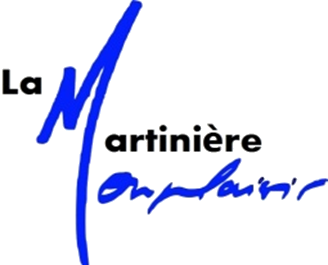
\includegraphics[width=2cm]{logo_lycee.png}%
 \end{minipage}}

\fancyhead[C]{\rule{8cm}{.5pt}}

 \fancyhead[R]{%
 \noindent\begin{minipage}[c]{3cm}
 \begin{flushright}
 \footnotesize{\textit{\textsf{\xxtete}}}%
 \end{flushright}
 \end{minipage}
}

 \fancyfoot{}
 % PIEDS de page
\fancyfoot[C]{\rule{12cm}{.5pt}}
\renewcommand{\footrulewidth}{0.2pt}
\fancyfoot[C]{\footnotesize{\bfseries \thepage}}
\fancyfoot[L]{ 
\begin{minipage}[c]{.4\linewidth}
\noindent\footnotesize{{\xxauteur}}
\end{minipage}}

\fancyfoot[R]{\footnotesize{\xxpied}
\ifthenelse{\isodd{\value{page}}}{
\begin{tikzpicture}[overlay]
\node[shape=rectangle, 
      rounded corners = .25 cm,
	  draw= ocre,
	  line width=2pt, 
	  fill = ocre!10,
	  minimum width  = 2.5cm,
	  minimum height = 3cm,] at (\xxposongletx,\xxposonglety) {};
\node at (\xxposonglettext,\xxposonglety) {\rotatebox{90}{\textbf{\large\color{ocre}{\xxonglet}}}};
%{};
\end{tikzpicture}}{}
}



%
%
%
% Removes the header from odd empty pages at the end of chapters
\makeatletter
%\renewcommand{\cleardoublepage}{
%\clearpage\ifodd\c@page\else
%\hbox{}
%\vspace*{\fill}
%\thispagestyle{empty}
%\newpage
%\fi}

%\fancypagestyle{plain}{%
%\fancyhf{} % vide l’en-tête et le pied~de~page.
%%\fancyfoot[C]{\bfseries \thepage} % numéro de la page en cours en gras
%% et centré en pied~de~page.
%\fancyfoot[R]{\footnotesize{\xxpied}}
%\fancyfoot[C]{\rule{12cm}{.5pt}}
%\renewcommand{\footrulewidth}{0.2pt}
%\fancyfoot[C]{\footnotesize{\bfseries \thepage}}
%\fancyfoot[L]{ 
%\begin{minipage}[c]{.4\linewidth}
%\noindent\footnotesize{{\xxauteur}}
%\end{minipage}}}

\fancypagestyle{plain}{%
\fancyhf{} % vide l’en-tête et le pied~de~page.
\fancyfoot[C]{\rule{12cm}{.5pt}}
\renewcommand{\footrulewidth}{0.2pt}
\fancyfoot[C]{\footnotesize{\bfseries \thepage}}
\fancyfoot[L]{ 
\begin{minipage}[c]{.4\linewidth}
\noindent\footnotesize{{\xxauteur}}
\end{minipage}}
\fancyfoot[R]{\footnotesize{\xxpied}}
}



%----------------------------------------------------------------------------------------
%	THEOREM STYLES
%----------------------------------------------------------------------------------------

% Conflit avec la police adobe
%\usepackage{amsmath,amsfonts,amssymb,amsthm} % For math equations, theorems, symbols, etc
\usepackage{amsmath,amsthm}

\newcommand{\intoo}[2]{\mathopen{]}#1\,;#2\mathclose{[}}
\newcommand{\ud}{\mathop{\mathrm{{}d}}\mathopen{}}
\newcommand{\intff}[2]{\mathopen{[}#1\,;#2\mathclose{]}}
%\newtheorem{notation}{Notation}[chapter]
\newtheorem{notation}{Notation}[section]

% Boxed/framed environments
\newtheoremstyle{ocrenumbox}% % Theorem style name
{0pt}% Space above
{0pt}% Space below
{\normalfont}% % Body font
{}% Indent amount
{\small\bf\sffamily\color{ocre}}% % Theorem head font
{\;}% Punctuation after theorem head
{0.25em}% Space after theorem head
{\small\sffamily\color{ocre}\thmname{#1}\nobreakspace\thmnumber%{\@ifnotempty{#1}{}\@upn{#2}}% Theorem text (e.g. Theorem 2.1)
\thmnote{\nobreakspace\the\thm@notefont\sffamily\bfseries\color{black}---\nobreakspace#3.}} % Optional theorem note
\renewcommand{\qedsymbol}{$\blacksquare$}% Optional qed square


% Boite pour les corriges
\newtheoremstyle{correctionbox}% % Theorem style name
{0pt}% Space above
{0pt}% Space below
{\normalfont}% % Body font
{}% Indent amount
{\small\bf\sffamily\color{violet}}% % Theorem head font
{\;}% Punctuation after theorem head
{0.25em}% Space after theorem head
{\small\sffamily\color{ocre}\thmname{#1}\nobreakspace\thmnumber%{\@ifnotempty{#1}{}\@upn{#2}}% Theorem text (e.g. Theorem 2.1)
\thmnote{\nobreakspace\the\thm@notefont\sffamily\bfseries\color{black}---\nobreakspace#3.}} % Optional theorem note
\renewcommand{\qedsymbol}{$\blacksquare$}% Optional qed square



\newtheoremstyle{blacknumex}% Theorem style name
{5pt}% Space above
{5pt}% Space below
{\normalfont}% Body font
{} % Indent amount
{\small\bf\sffamily}% Theorem head font
{\;}% Punctuation after theorem head
{0.25em}% Space after theorem head
{\small\sffamily{\tiny\ensuremath{\blacksquare}}\nobreakspace\thmname{#1}\nobreakspace\thmnumber%{\@ifnotempty{#1}{}\@upn{#2}}% Theorem text (e.g. Theorem 2.1)
\thmnote{\nobreakspace\the\thm@notefont\sffamily\bfseries---\nobreakspace#3.}}% Optional theorem note

\newtheoremstyle{blacknumbox} % Theorem style name
{0pt}% Space above
{0pt}% Space below
{\normalfont}% Body font
{}% Indent amount
{\small\bf\sffamily}% Theorem head font
{\;}% Punctuation after theorem head
{0.25em}% Space after theorem head
{\small\sffamily\thmname{#1}\nobreakspace 
\thmnote{\nobreakspace\the\thm@notefont\sffamily\bfseries---\nobreakspace#3.}}% Optional theorem note

% Non-boxed/non-framed environments
\newtheoremstyle{ocrenum}% % Theorem style name
{5pt}% Space above
{5pt}% Space below
{\normalfont}% % Body font
{}% Indent amount
{\small\bf\sffamily\color{ocre}}% % Theorem head font
{\;}% Punctuation after theorem head
{0.25em}% Space after theorem head
{\small\sffamily\color{ocre}\thmname{#1}\nobreakspace%\thmnumber{\@ifnotempty{#1}{}\@upn{#2}}% Theorem text (e.g. Theorem 2.1)
\thmnote{\nobreakspace\the\thm@notefont\sffamily\bfseries\color{black}---\nobreakspace#3.}} % Optional theorem note
\renewcommand{\qedsymbol}{$\blacksquare$}% Optional qed square
\makeatother

% Environnement pour les titres de parties
\newtheoremstyle{partiebox} 
{0pt}% Space above
{0pt}% Space below
{\normalfont}% Body font
{}% Indent amount
{\small\bf\sffamily}% Theorem head font
{\;}% Punctuation after theorem head
{0.25em}% Space after theorem head




% Defines the theorem text style for each type of theorem to one of the three styles above
\newcounter{dummy} 
\numberwithin{dummy}{section}
\theoremstyle{ocrenumbox}
%\newtheorem{theoremeT}[dummy]{Théorème}
\newtheorem{theoremeT}[dummy]{Théorème}
\newtheorem{resultatT}[dummy]{Résultat}
\newtheorem{savoirT}[dummy]{Savoir}
\newtheorem{methodeT}[dummy]{Méthode}
\newtheorem{objectifT}[dummy]{Objectif}
%\newtheorem{problem}{Problem}[chapter]
\newtheorem{problem}{Problem}[section]
%\newtheorem{exerciseT}{Exercise}[chapter]
\newtheorem{exerciseT}{Exercice}[section]

\theoremstyle{blacknumex}
%\newtheorem{exampleT}{Example}[chapter]
\newtheorem{exempleT}{Exemple}[section]
\newtheorem{termT}{Terminal\\}[section]
\newtheorem{pyT}{Python\\}[section]
\newtheorem{sciT}{Scilab\\}[section]
\newtheorem{pseudoT}{Pseudo Code\\}[section]
\newtheorem{sqlT}{SQL\\}[section]

\theoremstyle{blacknumbox}
%\newtheorem{vocabulary}{Vocabulary}[chapter]
\newtheorem{vocabulary}{Vocabulaire}[section]
%\newtheorem{definitionT}{Definition}[section]
\newtheorem{definitionT}{Définition}[section]
\newtheorem{rappelT}{Rappel}[section]
\newtheorem{demoT}{Démonstration}[section]
\newtheorem{corollaryT}[dummy]{Corollaire}
\newtheorem{hypoT}{Hypothèse(s)}

\theoremstyle{ocrenum}
\newtheorem{proposition}[dummy]{Proposition}

\theoremstyle{partiebox}
\newtheorem{titrepartieT}[]{}
\newtheorem{titrechapitreT}[]{}

\theoremstyle{correctionbox}
\newtheorem{correctionT}[dummy]{\color{violet}{Correction}}

%----------------------------------------------------------------------------------------
%	DEFINITION OF COLORED BOXES
%----------------------------------------------------------------------------------------

\RequirePackage[framemethod=tikz]{mdframed} % Required for creating the theorem, definition, exercise and corollary boxes

% Theorem box
\newmdenv[skipabove=7pt,
skipbelow=7pt,
backgroundcolor=ocre!10,
linecolor=ocre,
innerleftmargin=5pt,
innerrightmargin=5pt,
innertopmargin=5pt,
leftmargin=0cm,
rightmargin=0cm,
innerbottommargin=5pt]{tBox}


% Correction
\newmdenv[skipabove=7pt,
skipbelow=7pt,
backgroundcolor=violet!10,
linecolor=violet,
innerleftmargin=5pt,
innerrightmargin=5pt,
innertopmargin=5pt,
leftmargin=0cm,
rightmargin=0cm,
innerbottommargin=5pt]{coBox}


% Exercise box	  
\newmdenv[skipabove=7pt,
skipbelow=7pt,
rightline=false,
leftline=true,
topline=false,
bottomline=false,
backgroundcolor=ocre!10,
linecolor=ocre,
innerleftmargin=5pt,
innerrightmargin=5pt,
innertopmargin=5pt,
innerbottommargin=5pt,
leftmargin=0cm,
rightmargin=0cm,
linewidth=4pt]{eBox}	

% Definition box
\newmdenv[skipabove=7pt,
skipbelow=7pt,
rightline=false,
leftline=true,
topline=false,
bottomline=false,
backgroundcolor=ocre!10,
linecolor=ocre,
innerleftmargin=5pt,
innerrightmargin=5pt,
innertopmargin=0pt,
leftmargin=0cm,
rightmargin=0cm,
linewidth=4pt,
innerbottommargin=0pt]{dBox}	

% Demonstration box
\newmdenv[skipabove=7pt,
skipbelow=7pt,
rightline=false,
leftline=true,
topline=false,
bottomline=false,
%backgroundcolor=ocre!10,
linecolor=ocre,
innerleftmargin=5pt,
innerrightmargin=5pt,
innertopmargin=0pt,
leftmargin=0cm,
rightmargin=0cm,
linewidth=4pt,
innerbottommargin=0pt]{demoBox}	

% Corollary box
\newmdenv[skipabove=7pt,
skipbelow=7pt,
rightline=false,
leftline=true,
topline=false,
bottomline=false,
linecolor=gray,
backgroundcolor=black!5,
innerleftmargin=5pt,
innerrightmargin=5pt,
innertopmargin=5pt,
leftmargin=0cm,
rightmargin=0cm,
linewidth=4pt,
innerbottommargin=5pt]{cBox}


% Hypothèses
\newmdenv[skipabove=7pt,
skipbelow=7pt,
rightline=false,
leftline=true,
topline=false,
bottomline=false,
linecolor=gray,
backgroundcolor=black!5,
innerleftmargin=5pt,
innerrightmargin=5pt,
innertopmargin=5pt,
leftmargin=0cm,
rightmargin=0cm,
linewidth=4pt,
innerbottommargin=5pt]{hyBox}


% Boite pour le titre de la partie (pBox)
\newmdenv[skipabove=7pt,
skipbelow=7pt,
rightline=true,
leftline=false,
topline=false,
bottomline=false,
linecolor=ocre,
backgroundcolor=none,
innerleftmargin=5pt,
innerrightmargin=5pt,
innertopmargin=5pt,
leftmargin=0cm,
rightmargin=0cm,
linewidth=4pt,
innerbottommargin=5pt]{pBox}

% Boite pour le titre du chapitre (chBox)
\newmdenv[skipabove=7pt,
skipbelow=7pt,
rightline=false,
leftline=true,
topline=false,
bottomline=false,
linecolor=ocre,
%backgroundcolor=black!5,
innerleftmargin=5pt,
innerrightmargin=5pt,
innertopmargin=5pt,
leftmargin=0cm,
rightmargin=0cm,
linewidth=4pt,
innerbottommargin=5pt]{chBox}


% Boite pour les exemples
\newmdenv[skipabove=7pt,
skipbelow=7pt,
rightline=false,
leftline=true,
topline=false,
bottomline=false,
linecolor=gray,
backgroundcolor=white,
innerleftmargin=5pt,
innerrightmargin=5pt,
innertopmargin=5pt,
leftmargin=0cm,
rightmargin=0cm,
linewidth=4pt,
innerbottommargin=5pt]{exBox}

% Boite pour le terminal
\newmdenv[skipabove=7pt,
skipbelow=7pt,
rightline=false,
leftline=true,
topline=false,
bottomline=false,
linecolor=gray,
backgroundcolor=white,
innerleftmargin=5pt,
innerrightmargin=5pt,
innertopmargin=5pt,
leftmargin=0cm,
rightmargin=0cm,
linewidth=4pt,
innerbottommargin=5pt]{termBox}


% Boite pour Python
\newmdenv[skipabove=7pt,
skipbelow=7pt,
rightline=false,
leftline=true,
topline=false,
bottomline=false,
linecolor=gray,
backgroundcolor=white,
innerleftmargin=5pt,
innerrightmargin=5pt,
innertopmargin=0pt,
leftmargin=0cm,
rightmargin=0cm,
linewidth=4pt,
innerbottommargin=5pt]{pyBox}

% Boite pour scilab
\newmdenv[skipabove=7pt,
skipbelow=7pt,
rightline=false,
leftline=true,
topline=false,
bottomline=false,
linecolor=gray,
backgroundcolor=white,
innerleftmargin=5pt,
innerrightmargin=5pt,
innertopmargin=5pt,
leftmargin=0cm,
rightmargin=0cm,
linewidth=4pt,
innerbottommargin=5pt]{sciBox}


% Boite pour pseudo
\newmdenv[skipabove=7pt,
skipbelow=7pt,
rightline=false,
leftline=true,
topline=false,
bottomline=false,
linecolor=gray,
backgroundcolor=white,
innerleftmargin=5pt,
innerrightmargin=5pt,
innertopmargin=5pt,
leftmargin=0cm,
rightmargin=0cm,
linewidth=4pt,
innerbottommargin=5pt]{pseudoBox}

% Boite pour pseudo
\newmdenv[skipabove=7pt,
skipbelow=7pt,
rightline=false,
leftline=true,
topline=false,
bottomline=false,
linecolor=gray,
backgroundcolor=white,
innerleftmargin=5pt,
innerrightmargin=5pt,
innertopmargin=5pt,
leftmargin=0cm,
rightmargin=0cm,
linewidth=4pt,
innerbottommargin=5pt]{sqlBox}


% Creates an environment for each type of theorem and assigns it a theorem text style from the "Theorem Styles" section above and a colored box from above
\newenvironment{theorem}{\begin{tBox}\begin{theoremeT}}{\end{theoremeT}\end{tBox}}
\newenvironment{resultat}{\begin{tBox}\begin{resultatT}}{\end{resultatT}\end{tBox}}
\newenvironment{methode}{\begin{tBox}\begin{methodeT}}{\end{methodeT}\end{tBox}}
\newenvironment{savoir}{\begin{tBox}\begin{savoirT}}{\end{savoirT}\end{tBox}}
\newenvironment{obj}{\begin{tBox}\begin{objectifT}}{\end{objectifT}\end{tBox}}
\newenvironment{corrige}{\begin{coBox}\begin{correctionT}}{\end{correctionT}\end{coBox}}
\newenvironment{exercise}{\begin{eBox}\begin{exerciseT}}{\hfill{\color{ocre}\tiny\ensuremath{\blacksquare}}\end{exerciseT}\end{eBox}}				  
\newenvironment{exercice}{\begin{eBox}\begin{exerciseT}}{\hfill{\color{ocre}\tiny\ensuremath{\blacksquare}}\end{exerciseT}\end{eBox}}				  

\newenvironment{definition}{\begin{dBox}\begin{definitionT}}{\end{definitionT}\end{dBox}}	
\newenvironment{rappel}{\begin{dBox}\begin{rappelT}}{\end{rappelT}\end{dBox}}	
\newenvironment{defi}{\begin{dBox}\begin{definitionT}}{\end{definitionT}\end{dBox}}	
\newenvironment{demo}{\begin{demoBox}\begin{demoT}}{\end{demoT}\end{demoBox}}	
%\newenvironment{exemple}{\begin{exempleT}}{\hfill{\tiny\ensuremath{\blacksquare}}\end{exempleT}}		
\newenvironment{corollary}{\begin{cBox}\begin{corollaryT}}{\end{corollaryT}\end{cBox}}
\newenvironment{hypo}{\begin{hyBox}\begin{hypoT}}{\end{hypoT}\end{hyBox}}	\newenvironment{exemple}{\begin{exBox}\begin{exempleT}}{\hfill{\tiny\ensuremath{\blacksquare}}\end{exempleT}\end{exBox}}	
\newenvironment{titrepartie}{\begin{pBox}\begin{titrepartieT}}{\end{titrepartieT}\end{pBox}}	
\newenvironment{titrechapitre}{\begin{chBox}\begin{titrechapitreT}}{\end{titrechapitreT}\end{chBox}}	

\newenvironment{term}{ \begin{termBox}\begin{termT}}{\end{termT}\end{termBox}}
\newenvironment{py}{ \begin{pyBox}\begin{pyT}}{\end{pyT}\end{pyBox}}
\newenvironment{sci}{ \begin{sciBox}\begin{sciT}}{\end{sciT}\end{sciBox}}
\newenvironment{pseudo}{ \begin{pseudoBox}\begin{pseudoT}}{\end{pseudoT}\end{pseudoBox}}
\newenvironment{envsql}{ \begin{sqlBox}\begin{sqlT}}{\end{sqlT}\end{sqlBox}}


%----------------------------------------------------------------------------------------
%	REMARK ENVIRONMENT
%----------------------------------------------------------------------------------------

\newenvironment{remark}{\par\vspace{10pt}\small % Vertical white space above the remark and smaller font size
\begin{list}{}{
\leftmargin=35pt % Indentation on the left
\rightmargin=25pt}\item\ignorespaces % Indentation on the right
\makebox[-2.5pt]{\begin{tikzpicture}[overlay]
\node[draw=ocre!60,line width=1pt,circle,fill=ocre!25,font=\sffamily\bfseries,inner sep=2pt,outer sep=0pt] at (-15pt,0pt){\textcolor{ocre}{R}};\end{tikzpicture}} % Orange R in a circle
\advance\baselineskip -1pt}{\end{list}\vskip5pt} % Tighter line spacing and white space after remark

\newenvironment{rem}{\par\vspace{10pt}\small % Vertical white space above the remark and smaller font size
\begin{list}{}{
\leftmargin=35pt % Indentation on the left
\rightmargin=25pt}\item\ignorespaces % Indentation on the right
\makebox[-2.5pt]{\begin{tikzpicture}[overlay]
\node[draw=ocre!60,line width=1pt,circle,fill=ocre!25,font=\sffamily\bfseries,inner sep=2pt,outer sep=0pt] at (-15pt,0pt){\textcolor{ocre}{R}};\end{tikzpicture}} % Orange R in a circle
\advance\baselineskip -1pt}{\end{list}\vskip5pt} % Tighter line spacing and white space after remark


\newenvironment{warn}{\par\vspace{10pt}\small % Vertical white space above the remark and smaller font size
\begin{list}{}{
\leftmargin=35pt % Indentation on the left
\rightmargin=25pt}\item\ignorespaces % Indentation on the right
\makebox[-2.5pt]{\begin{tikzpicture}[overlay]
\node[draw=red!60,line width=1pt,circle,fill=red!25,font=\sffamily\bfseries,inner sep=2pt,outer sep=0pt] at (-15pt,0pt){\textcolor{black}{!}};\end{tikzpicture}} % Point d'exclamation dans un cercle
\advance\baselineskip -1pt}{\end{list}\vskip5pt} % Tighter line spacing and white space after remark


%----------------------------------------------------------------------------------------
%	SECTION NUMBERING IN THE MARGIN
%----------------------------------------------------------------------------------------
\setcounter{secnumdepth}{3}
\setcounter{tocdepth}{2}



\makeatletter
\renewcommand{\@seccntformat}[1]{\llap{\textcolor{ocre}{\csname the#1\endcsname}\hspace{1em}}}                    
\renewcommand{\section}{\@startsection{section}{1}{\z@}
{-4ex \@plus -1ex \@minus -.4ex}
{1ex \@plus.2ex }
{\normalfont\large\sffamily\bfseries}}
\renewcommand{\subsection}{\@startsection {subsection}{2}{\z@}
{-3ex \@plus -0.1ex \@minus -.4ex}
{0.5ex \@plus.2ex }
{\normalfont\sffamily\bfseries}}
\renewcommand{\subsubsection}{\@startsection {subsubsection}{3}{\z@}
{-2ex \@plus -0.1ex \@minus -.2ex}
{.2ex \@plus.2ex }
{\normalfont\small\sffamily\bfseries}}                        
\renewcommand\paragraph{\@startsection{paragraph}{4}{\z@}
{-2ex \@plus-.2ex \@minus .2ex}
{.1ex}
{\normalfont\small\sffamily\bfseries}}

%----------------------------------------------------------------------------------------
%	PART HEADINGS
%----------------------------------------------------------------------------------------


%----------------------------------------------------------------------------------------
%	CHAPTER HEADINGS
%----------------------------------------------------------------------------------------

% \newcommand{\thechapterimage}{}%
% \newcommand{\chapterimage}[1]{\renewcommand{\thechapterimage}{#1}}%
% \def\@makechapterhead#1{%
% {\parindent \z@ \raggedright \normalfont
% \ifnum \c@secnumdepth >\m@ne
% \if@mainmatter
% \begin{tikzpicture}[remember picture,overlay]
% \node at (current page.north west)
% {\begin{tikzpicture}[remember picture,overlay]
% \node[anchor=north west,inner sep=0pt] at (0,0) {\includegraphics[width=\paperwidth]{\thechapterimage}};
% \draw[anchor=west] (\Gm@lmargin,-9cm) node [line width=2pt,rounded corners=15pt,draw=ocre,fill=white,fill opacity=0.5,inner sep=15pt]{\strut\makebox[22cm]{}};
% \draw[anchor=west] (\Gm@lmargin+.3cm,-9cm) node {\huge\sffamily\bfseries\color{black}\thechapter. #1\strut};
% \end{tikzpicture}};
% \end{tikzpicture}
% \else
% \begin{tikzpicture}[remember picture,overlay]
% \node at (current page.north west)
% {\begin{tikzpicture}[remember picture,overlay]
% \node[anchor=north west,inner sep=0pt] at (0,0) {\includegraphics[width=\paperwidth]{\thechapterimage}};
% \draw[anchor=west] (\Gm@lmargin,-9cm) node [line width=2pt,rounded corners=15pt,draw=ocre,fill=white,fill opacity=0.5,inner sep=15pt]{\strut\makebox[22cm]{}};
% \draw[anchor=west] (\Gm@lmargin+.3cm,-9cm) node {\huge\sffamily\bfseries\color{black}#1\strut};
% \end{tikzpicture}};
% \end{tikzpicture}
% \fi\fi\par\vspace*{270\p@}}}

%-------------------------------------------

\def\@makeschapterhead#1{%
\begin{tikzpicture}[remember picture,overlay]
\node at (current page.north west)
{\begin{tikzpicture}[remember picture,overlay]
\node[anchor=north west,inner sep=0pt] at (0,0) {\includegraphics[width=\paperwidth]{\thechapterimage}};
\draw[anchor=west] (\Gm@lmargin,-9cm) node [line width=2pt,rounded corners=15pt,draw=ocre,fill=white,fill opacity=0.5,inner sep=15pt]{\strut\makebox[22cm]{}};
\draw[anchor=west] (\Gm@lmargin+.3cm,-9cm) node {\huge\sffamily\bfseries\color{black}#1\strut};
\end{tikzpicture}};
\end{tikzpicture}
\par\vspace*{270\p@}}
\makeatother

%----------------------------------------------------------------------------------------
%	HYPERLINKS IN THE DOCUMENTS
%----------------------------------------------------------------------------------------


\hypersetup{hidelinks,backref=true,pagebackref=true,hyperindex=true,colorlinks=false,breaklinks=true,urlcolor= ocre,bookmarks=true,bookmarksopen=false,pdftitle={Title},pdfauthor={Author}}
\usepackage{bookmark}
\bookmarksetup{
open,
numbered,
addtohook={%
\ifnum\bookmarkget{level}=0 % chapter
\bookmarksetup{bold}%
\fi
\ifnum\bookmarkget{level}=-1 % part
\bookmarksetup{color=ocre,bold}%
\fi
}
}

%----------------------------------------------------------------------------------------
%	
%----------------------------------------------------------------------------------------

\newcommand{\thechapterimage}{}%
\newcommand{\chapterimage}[1]{\renewcommand{\thechapterimage}{#1}}%
\def\@makechapterhead#1{%
{\parindent \z@ \raggedright \normalfont
\begin{tikzpicture}[remember picture,overlay]
\node at (current page.north west)
{\begin{tikzpicture}[remember picture,overlay]
\node[anchor=north west,inner sep=0pt] at (0,0) {\includegraphics[width=\paperwidth]{\thechapterimage}};
%\draw[anchor=west] (\Gm@lmargin,-9cm) node [line width=2pt,rounded corners=15pt,draw=ocre,fill=white,fill opacity=0.5,inner sep=15pt]{\strut\makebox[22cm]{}};
%\draw[anchor=west] (\Gm@lmargin+.3cm,-9cm) node {\huge\sffamily\bfseries\color{black}\thechapter. #1\strut};
\end{tikzpicture}};
\end{tikzpicture}
\par\vspace*{270\p@}
}}

 \newcounter{exo}


\makeatletter             
\renewcommand{\subparagraph}{\@startsection{exo}{5}{\z@}%
                                    {-2ex \@plus-.2ex \@minus .2ex}%
                                    {0ex}%               
{\normalfont\bfseries Question \hspace{.7cm} }}
\makeatother
\renewcommand{\thesubparagraph}{\arabic{subparagraph}} 
\makeatletter


\usepackage{textcomp}

% Définition des booleéns
\newif\iffiche
\newif\ifprof
\newif\iftd
\newif\ifcours
\newif\ifnormal
\newif\ifdifficile
\newif\iftdifficile
\newif\ifcolle
\newif\iflivret
%%%%%%%%%%%%
% Définition des vecteurs 
%%%%%%%%%%%%
\newcommand{\vect}[1]{\overrightarrow{#1}}
\newcommand{\axe}[2]{\left(#1,\vect{#2}\right)}
\newcommand{\couple}[2]{\left(#1,\vect{#2}\right)}
\newcommand{\angl}[2]{\left(\vect{#1},\vect{#2}\right)}

\newcommand{\rep}[1]{\mathcal{R}_{#1}}
\newcommand{\quadruplet}[4]{\left(#1;#2,#3,#4 \right)}
\newcommand{\repere}[4]{\left(#1;\vect{#2},\vect{#3},\vect{#4} \right)}
\newcommand{\base}[3]{\left(\vect{#1},\vect{#2},\vect{#3} \right)}


\newcommand{\vx}[1]{\vect{x_{#1}}}
\newcommand{\vy}[1]{\vect{y_{#1}}}
\newcommand{\vz}[1]{\vect{z_{#1}}}

% d droit pour le calcul différentiel
\newcommand{\dd}{\text{d}}

\newcommand{\inertie}[2]{I_{#1}\left( #2\right)}
\newcommand{\matinertie}[7]{
\begin{pmatrix}
#1 & #6 & #5 \\
#6 & #2 & #4 \\
#5 & #4 & #3 \\
\end{pmatrix}_{#7}}
%%%%%%%%%%%%
% Définition des torseurs 
%%%%%%%%%%%%

\newcommand{\ec}[2]{%
\mathcal{E}_c\left(#1/#2\right)}

\newcommand{\pext}[3]{%
\mathcal{P}\left(#1\rightarrow#2/#3\right)}

\newcommand{\pint}[3]{%
\mathcal{P}\left(#1 \stackrel{\text{#3}}{\leftrightarrow} #2\right)}


 \newcommand{\torseur}[1]{%
\left\{{#1}\right\}
}

\newcommand{\torseurcin}[3]{%
\left\{\mathcal{#1} \left(#2/#3 \right) \right\}
}

\newcommand{\torseurci}[2]{%
\left\{\sigma \left(#1/#2 \right) \right\}
}
\newcommand{\torseurdyn}[2]{%
\left\{\mathcal{D} \left(#1/#2 \right) \right\}
}


\newcommand{\torseurstat}[3]{%
\left\{\mathcal{#1} \left(#2\rightarrow #3 \right) \right\}
}


 \newcommand{\torseurc}[8]{%
%\left\{#1 \right\}=
\left\{
{#1}
\right\}
 = 
\left\{%
\begin{array}{cc}%
{#2} & {#5}\\%
{#3} & {#6}\\%
{#4} & {#7}\\%
\end{array}%
\right\}_{#8}%
}

 \newcommand{\torseurcol}[7]{
\left\{%
\begin{array}{cc}%
{#1} & {#4}\\%
{#2} & {#5}\\%
{#3} & {#6}\\%
\end{array}%
\right\}_{#7}%
}

 \newcommand{\torseurl}[3]{%
%\left\{\mathcal{#1}\right\}_{#2}=%
\left\{%
\begin{array}{l}%
{#1} \\%
{#2} %
\end{array}%
\right\}_{#3}%
}

% Vecteur vitesse
 \newcommand{\vectv}[3]{%
\vect{V\left( {#1} \in {#2}/{#3}\right)}
}

% Vecteur force
\newcommand{\vectf}[2]{%
\vect{R\left( {#1} \rightarrow {#2}\right)}
}

% Vecteur moment stat
\newcommand{\vectm}[3]{%
\vect{\mathcal{M}\left( {#1}, {#2} \rightarrow {#3}\right)}
}




% Vecteur résultante cin
\newcommand{\vectrc}[2]{%
\vect{R_c \left( {#1}/ {#2}\right)}
}
% Vecteur moment cin
\newcommand{\vectmc}[3]{%
\vect{\sigma \left( {#1}, {#2} /{#3}\right)}
}


% Vecteur résultante dyn
\newcommand{\vectrd}[2]{%
\vect{R_d \left( {#1}/ {#2}\right)}
}
% Vecteur moment dyn
\newcommand{\vectmd}[3]{%
\vect{\delta \left( {#1}, {#2} /{#3}\right)}
}

% Vecteur accélération
 \newcommand{\vectg}[3]{%
\vect{\Gamma \left( {#1} \in {#2}/{#3}\right)}
}

% Vecteur omega
 \newcommand{\vecto}[2]{%
\vect{\Omega\left( {#1}/{#2}\right)}
}
% }$$\left\{\mathcal{#1} \right\}_{#2} =%
% \left\{%
% \begin{array}{c}%
%  #3 \\%
%  #4 %
% \end{array}%
% \right\}_{#5}}
% -------------------------------------
% Déclaration des titres
% -------------------------------------

\def\discipline{Sciences \\Industrielles de \\ l'Ingénieur}
\def\xxtete{Sciences Industrielles de l'Ingénieur}

\def\classe{\textsf{PSI$\star$ -- MP}}
\def\xxnumpartie{Cycle 02}
\def\xxpartie{Modéliser les systèmes asservis dans le but de prévoir leur comportement}

\def\xxposongletx{2}
\def\xxposonglettext{1.45}
\def\xxposonglety{19}%16

\def\xxonglet{\textsf{Cycle 02}}
\def\xxauteur{\textsl{Xavier Pessoles}}
\def\xxactivite{Cours}

\def\xxpied{%
\xxnumpartie -- Modéliser les SLCI pour prévoir leur comportement\\
\xxnumchapitre -- \xxactivite%
}

\setcounter{secnumdepth}{5}
\chapterimage{Fond_SLCI}
%---------------------------------------------------------------------------




\def\xxYCartouche{-2.25cm}
\def\xxYongletGarde{.9cm}
\def\xxYOnget{.9cm}

\livrettrue

\begin{document}
% Cours
\graphicspath{{../../style/png/}{../../Chapitre_03_Precision/Cours/images/}}
\documentclass[10pt,fleqn]{article} % Default font size and left-justified equations
\usepackage[%
    pdftitle={Modélisation SLCI : Précision des systèmes},
    pdfauthor={Xavier Pessoles}]{hyperref}

%%%%%%%%%%%%%%%%%%%%%%%%%%%%%%%%%%%%%%%%%
% Original author:
% Mathias Legrand (legrand.mathias@gmail.com) with modifications by:
% Vel (vel@latextemplates.com)
% License:
% CC BY-NC-SA 3.0 (http://creativecommons.org/licenses/by-nc-sa/3.0/)
%%%%%%%%%%%%%%%%%%%%%%%%%%%%%%%%%%%%%%%%%

%----------------------------------------------------------------------------------------
%	VARIOUS REQUIRED PACKAGES AND CONFIGURATIONS
%----------------------------------------------------------------------------------------

%\usepackage[top=2.5cm,bottom=2cm,left=2cm,right=2cm,headsep=40pt,a4paper]{geometry} % Page margins
\usepackage[top=2cm,bottom=3cm,left=2cm,right=2cm,a4paper]{geometry} % Page margins

\usepackage{graphicx} % Required for including pictures

\usepackage{lipsum} % Inserts dummy text

\usepackage{tikz} % Required for drawing custom shapes

\usepackage[francais]{babel} % English language/hyphenation
\frenchbsetup{StandardLists=true} % Pour éviter la collision babel enumitem pour les listes

\usepackage{enumitem} % Customize lists
\setlist{nolistsep} % Reduce spacing between bullet points and numbered lists

\usepackage{booktabs} % Required for nicer horizontal rules in tables

\usepackage{xcolor} % Required for specifying colors by name
%\definecolor{ocre}{RGB}{243,102,25} % Define the orange color used for highlighting throughout the book
 \definecolor{ocre}{RGB}{49,133,156} % Couleur ''bleue''
\definecolor{violetf}{RGB}{112,48,160} % Couleur ''violet''
\usepackage{enumitem}
\usepackage{pifont} % Pour les dinglist
\usepackage{multicol}
\usepackage{array} % Centrage vertical dans les tableaux

%----------------------------------------------------------------------------------------
%	FONTS
%----------------------------------------------------------------------------------------

\usepackage{multicol}
\usepackage{siunitx}
\sisetup{output-decimal-marker = {,}}


\usepackage{avant} % Use the Avantgarde font for headings
%\usepackage{times} % Use the Times font for headings
%\usepackage{mathptmx} % Use the Adobe Times Roman as the default text font together with math symbols from the Sym­bol, Chancery and Com­puter Modern fonts
\usepackage[adobe-utopia]{mathdesign}
\usepackage{microtype} % Slightly tweak font spacing for aesthetics
\usepackage[utf8]{inputenc} % Required for including letters with accents
\usepackage[T1]{fontenc} % Use 8-bit encoding that has 256 glyphs

%----------------------------------------------------------------------------------------
%	BIBLIOGRAPHY AND INDEX
%----------------------------------------------------------------------------------------

%\usepackage[style=alphabetic,citestyle=numeric,sorting=nyt,sortcites=true,autopunct=true,babel=hyphen,hyperref=true,abbreviate=false,backref=true,backend=biber]{biblatex}
\usepackage[style=alphabetic,citestyle=numeric,sorting=nyt,sortcites=true,autopunct=true,hyperref=true,abbreviate=false,backref=true,backend=biber]{biblatex}
\addbibresource{bibliography.bib} % BibTeX bibliography file
\defbibheading{bibempty}{}

\usepackage{calc} % For simpler calculation - used for spacing the index letter headings correctly
\usepackage{makeidx} % Required to make an index
\makeindex % Tells LaTeX to create the files required for indexing

%----------------------------------------------------------------------------------------
%	MAIN TABLE OF CONTENTS
%----------------------------------------------------------------------------------------

\usepackage{titletoc} % Required for manipulating the table of contents

\setcounter{tocdepth}{2}     % Dans la table des matieres
\setcounter{secnumdepth}{2}

\contentsmargin{0cm} % Removes the default margin

% Part text styling
\titlecontents{part}[0cm]
{\addvspace{20pt}\centering\large\bfseries}
{}
{}
{}

% Chapter text styling
\titlecontents{chapter}[1.25cm] % Indentation
{\addvspace{12pt}\large\sffamily\bfseries} % Spacing and font options for chapters
{\color{ocre!60}\contentslabel[\Large\thecontentslabel]{1.25cm}\color{ocre}} % Chapter number
{\color{ocre}}  
{\color{ocre!60}\normalsize\;\titlerule*[.5pc]{.}\;\thecontentspage} % Page number

% Section text styling
\titlecontents{section}[1.25cm] % Indentation
{\addvspace{3pt}\sffamily\bfseries} % Spacing and font options for sections
{\color{ocre!60}\contentslabel[\thecontentslabel]{1.25cm} \color{ocre}} % Section number
{\color{ocre}}
{\hfill\color{ocre!60}\thecontentspage} % Page number
[]

% Subsection text styling
\titlecontents{subsection}[1.25cm] % Indentation
{\addvspace{1pt}\sffamily\small} % Spacing and font options for subsections
{\contentslabel[\thecontentslabel]{1.25cm}} % Subsection number
{}
{\ \titlerule*[.5pc]{.}\;\thecontentspage} % Page number
[]


% Subsection text styling
\titlecontents{subsubsection}[1.25cm] % Indentation
{\addvspace{1pt}\sffamily\small} % Spacing and font options for subsections
{\contentslabel[\thecontentslabel]{1.25cm}} % Subsection number
{}
{\ \titlerule*[.5pc]{.}\;\thecontentspage} % Page number
[]

% List of figures
\titlecontents{figure}[0em]
{\addvspace{-5pt}\sffamily}
{\thecontentslabel\hspace*{1em}}
{}
{\ \titlerule*[.5pc]{.}\;\thecontentspage}
[]

% List of tables
\titlecontents{table}[0em]
{\addvspace{-5pt}\sffamily}
{\thecontentslabel\hspace*{1em}}
{}
{\ \titlerule*[.5pc]{.}\;\thecontentspage}
[]

%----------------------------------------------------------------------------------------
%	MINI TABLE OF CONTENTS IN PART HEADS
%----------------------------------------------------------------------------------------

% Chapter text styling
\titlecontents{lchapter}[0em] % Indenting
{\addvspace{15pt}\large\sffamily\bfseries} % Spacing and font options for chapters
{\color{ocre}\contentslabel[\Large\thecontentslabel]{1.25cm}\color{ocre}} % Chapter number
{}  
{\color{ocre}\normalsize\sffamily\bfseries\;\titlerule*[.5pc]{.}\;\thecontentspage} % Page number

% Section text styling
\titlecontents{lsection}[0em] % Indenting
{\sffamily\small} % Spacing and font options for sections
{\contentslabel[\thecontentslabel]{1.25cm}} % Section number
{}
{}

% Subsection text styling
\titlecontents{lsubsection}[.5em] % Indentation
{\normalfont\footnotesize\sffamily} % Font settings
{}
{}
{}

%----------------------------------------------------------------------------------------
%	PAGE HEADERS
%----------------------------------------------------------------------------------------

\usepackage{fancyhdr} % Required for header and footer configuration



\pagestyle{fancy}
 \renewcommand{\headrulewidth}{0pt}
 \fancyhead{}
 
 % ENTETES de page
 \fancyhead[L]{%
 \noindent\begin{minipage}[c]{2.6cm}%
 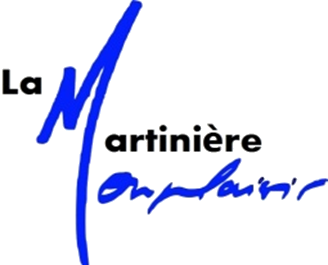
\includegraphics[width=2cm]{logo_lycee.png}%
 \end{minipage}}

\fancyhead[C]{\rule{8cm}{.5pt}}

 \fancyhead[R]{%
 \noindent\begin{minipage}[c]{3cm}
 \begin{flushright}
 \footnotesize{\textit{\textsf{\xxtete}}}%
 \end{flushright}
 \end{minipage}
}

 \fancyfoot{}
 % PIEDS de page
\fancyfoot[C]{\rule{12cm}{.5pt}}
\renewcommand{\footrulewidth}{0.2pt}
\fancyfoot[C]{\footnotesize{\bfseries \thepage}}
\fancyfoot[L]{ 
\begin{minipage}[c]{.4\linewidth}
\noindent\footnotesize{{\xxauteur}}
\end{minipage}}

\fancyfoot[R]{\footnotesize{\xxpied}
\ifthenelse{\isodd{\value{page}}}{
\begin{tikzpicture}[overlay]
\node[shape=rectangle, 
      rounded corners = .25 cm,
	  draw= ocre,
	  line width=2pt, 
	  fill = ocre!10,
	  minimum width  = 2.5cm,
	  minimum height = 3cm,] at (\xxposongletx,\xxposonglety) {};
\node at (\xxposonglettext,\xxposonglety) {\rotatebox{90}{\textbf{\large\color{ocre}{\xxonglet}}}};
%{};
\end{tikzpicture}}{}
}



%
%
%
% Removes the header from odd empty pages at the end of chapters
\makeatletter
%\renewcommand{\cleardoublepage}{
%\clearpage\ifodd\c@page\else
%\hbox{}
%\vspace*{\fill}
%\thispagestyle{empty}
%\newpage
%\fi}

%\fancypagestyle{plain}{%
%\fancyhf{} % vide l’en-tête et le pied~de~page.
%%\fancyfoot[C]{\bfseries \thepage} % numéro de la page en cours en gras
%% et centré en pied~de~page.
%\fancyfoot[R]{\footnotesize{\xxpied}}
%\fancyfoot[C]{\rule{12cm}{.5pt}}
%\renewcommand{\footrulewidth}{0.2pt}
%\fancyfoot[C]{\footnotesize{\bfseries \thepage}}
%\fancyfoot[L]{ 
%\begin{minipage}[c]{.4\linewidth}
%\noindent\footnotesize{{\xxauteur}}
%\end{minipage}}}

\fancypagestyle{plain}{%
\fancyhf{} % vide l’en-tête et le pied~de~page.
\fancyfoot[C]{\rule{12cm}{.5pt}}
\renewcommand{\footrulewidth}{0.2pt}
\fancyfoot[C]{\footnotesize{\bfseries \thepage}}
\fancyfoot[L]{ 
\begin{minipage}[c]{.4\linewidth}
\noindent\footnotesize{{\xxauteur}}
\end{minipage}}
\fancyfoot[R]{\footnotesize{\xxpied}}
}



%----------------------------------------------------------------------------------------
%	THEOREM STYLES
%----------------------------------------------------------------------------------------

% Conflit avec la police adobe
%\usepackage{amsmath,amsfonts,amssymb,amsthm} % For math equations, theorems, symbols, etc
\usepackage{amsmath,amsthm}

\newcommand{\intoo}[2]{\mathopen{]}#1\,;#2\mathclose{[}}
\newcommand{\ud}{\mathop{\mathrm{{}d}}\mathopen{}}
\newcommand{\intff}[2]{\mathopen{[}#1\,;#2\mathclose{]}}
%\newtheorem{notation}{Notation}[chapter]
\newtheorem{notation}{Notation}[section]

% Boxed/framed environments
\newtheoremstyle{ocrenumbox}% % Theorem style name
{0pt}% Space above
{0pt}% Space below
{\normalfont}% % Body font
{}% Indent amount
{\small\bf\sffamily\color{ocre}}% % Theorem head font
{\;}% Punctuation after theorem head
{0.25em}% Space after theorem head
{\small\sffamily\color{ocre}\thmname{#1}\nobreakspace\thmnumber%{\@ifnotempty{#1}{}\@upn{#2}}% Theorem text (e.g. Theorem 2.1)
\thmnote{\nobreakspace\the\thm@notefont\sffamily\bfseries\color{black}---\nobreakspace#3.}} % Optional theorem note
\renewcommand{\qedsymbol}{$\blacksquare$}% Optional qed square


% Boite pour les corriges
\newtheoremstyle{correctionbox}% % Theorem style name
{0pt}% Space above
{0pt}% Space below
{\normalfont}% % Body font
{}% Indent amount
{\small\bf\sffamily\color{violet}}% % Theorem head font
{\;}% Punctuation after theorem head
{0.25em}% Space after theorem head
{\small\sffamily\color{ocre}\thmname{#1}\nobreakspace\thmnumber%{\@ifnotempty{#1}{}\@upn{#2}}% Theorem text (e.g. Theorem 2.1)
\thmnote{\nobreakspace\the\thm@notefont\sffamily\bfseries\color{black}---\nobreakspace#3.}} % Optional theorem note
\renewcommand{\qedsymbol}{$\blacksquare$}% Optional qed square



\newtheoremstyle{blacknumex}% Theorem style name
{5pt}% Space above
{5pt}% Space below
{\normalfont}% Body font
{} % Indent amount
{\small\bf\sffamily}% Theorem head font
{\;}% Punctuation after theorem head
{0.25em}% Space after theorem head
{\small\sffamily{\tiny\ensuremath{\blacksquare}}\nobreakspace\thmname{#1}\nobreakspace\thmnumber%{\@ifnotempty{#1}{}\@upn{#2}}% Theorem text (e.g. Theorem 2.1)
\thmnote{\nobreakspace\the\thm@notefont\sffamily\bfseries---\nobreakspace#3.}}% Optional theorem note

\newtheoremstyle{blacknumbox} % Theorem style name
{0pt}% Space above
{0pt}% Space below
{\normalfont}% Body font
{}% Indent amount
{\small\bf\sffamily}% Theorem head font
{\;}% Punctuation after theorem head
{0.25em}% Space after theorem head
{\small\sffamily\thmname{#1}\nobreakspace 
\thmnote{\nobreakspace\the\thm@notefont\sffamily\bfseries---\nobreakspace#3.}}% Optional theorem note

% Non-boxed/non-framed environments
\newtheoremstyle{ocrenum}% % Theorem style name
{5pt}% Space above
{5pt}% Space below
{\normalfont}% % Body font
{}% Indent amount
{\small\bf\sffamily\color{ocre}}% % Theorem head font
{\;}% Punctuation after theorem head
{0.25em}% Space after theorem head
{\small\sffamily\color{ocre}\thmname{#1}\nobreakspace%\thmnumber{\@ifnotempty{#1}{}\@upn{#2}}% Theorem text (e.g. Theorem 2.1)
\thmnote{\nobreakspace\the\thm@notefont\sffamily\bfseries\color{black}---\nobreakspace#3.}} % Optional theorem note
\renewcommand{\qedsymbol}{$\blacksquare$}% Optional qed square
\makeatother

% Environnement pour les titres de parties
\newtheoremstyle{partiebox} 
{0pt}% Space above
{0pt}% Space below
{\normalfont}% Body font
{}% Indent amount
{\small\bf\sffamily}% Theorem head font
{\;}% Punctuation after theorem head
{0.25em}% Space after theorem head




% Defines the theorem text style for each type of theorem to one of the three styles above
\newcounter{dummy} 
\numberwithin{dummy}{section}
\theoremstyle{ocrenumbox}
%\newtheorem{theoremeT}[dummy]{Théorème}
\newtheorem{theoremeT}[dummy]{Théorème}
\newtheorem{resultatT}[dummy]{Résultat}
\newtheorem{savoirT}[dummy]{Savoir}
\newtheorem{methodeT}[dummy]{Méthode}
\newtheorem{objectifT}[dummy]{Objectif}
%\newtheorem{problem}{Problem}[chapter]
\newtheorem{problem}{Problem}[section]
%\newtheorem{exerciseT}{Exercise}[chapter]
\newtheorem{exerciseT}{Exercice}[section]

\theoremstyle{blacknumex}
%\newtheorem{exampleT}{Example}[chapter]
\newtheorem{exempleT}{Exemple}[section]
\newtheorem{termT}{Terminal\\}[section]
\newtheorem{pyT}{Python\\}[section]
\newtheorem{sciT}{Scilab\\}[section]
\newtheorem{pseudoT}{Pseudo Code\\}[section]
\newtheorem{sqlT}{SQL\\}[section]

\theoremstyle{blacknumbox}
%\newtheorem{vocabulary}{Vocabulary}[chapter]
\newtheorem{vocabulary}{Vocabulaire}[section]
%\newtheorem{definitionT}{Definition}[section]
\newtheorem{definitionT}{Définition}[section]
\newtheorem{rappelT}{Rappel}[section]
\newtheorem{demoT}{Démonstration}[section]
\newtheorem{corollaryT}[dummy]{Corollaire}
\newtheorem{hypoT}{Hypothèse(s)}

\theoremstyle{ocrenum}
\newtheorem{proposition}[dummy]{Proposition}

\theoremstyle{partiebox}
\newtheorem{titrepartieT}[]{}
\newtheorem{titrechapitreT}[]{}

\theoremstyle{correctionbox}
\newtheorem{correctionT}[dummy]{\color{violet}{Correction}}

%----------------------------------------------------------------------------------------
%	DEFINITION OF COLORED BOXES
%----------------------------------------------------------------------------------------

\RequirePackage[framemethod=tikz]{mdframed} % Required for creating the theorem, definition, exercise and corollary boxes

% Theorem box
\newmdenv[skipabove=7pt,
skipbelow=7pt,
backgroundcolor=ocre!10,
linecolor=ocre,
innerleftmargin=5pt,
innerrightmargin=5pt,
innertopmargin=5pt,
leftmargin=0cm,
rightmargin=0cm,
innerbottommargin=5pt]{tBox}


% Correction
\newmdenv[skipabove=7pt,
skipbelow=7pt,
backgroundcolor=violet!10,
linecolor=violet,
innerleftmargin=5pt,
innerrightmargin=5pt,
innertopmargin=5pt,
leftmargin=0cm,
rightmargin=0cm,
innerbottommargin=5pt]{coBox}


% Exercise box	  
\newmdenv[skipabove=7pt,
skipbelow=7pt,
rightline=false,
leftline=true,
topline=false,
bottomline=false,
backgroundcolor=ocre!10,
linecolor=ocre,
innerleftmargin=5pt,
innerrightmargin=5pt,
innertopmargin=5pt,
innerbottommargin=5pt,
leftmargin=0cm,
rightmargin=0cm,
linewidth=4pt]{eBox}	

% Definition box
\newmdenv[skipabove=7pt,
skipbelow=7pt,
rightline=false,
leftline=true,
topline=false,
bottomline=false,
backgroundcolor=ocre!10,
linecolor=ocre,
innerleftmargin=5pt,
innerrightmargin=5pt,
innertopmargin=0pt,
leftmargin=0cm,
rightmargin=0cm,
linewidth=4pt,
innerbottommargin=0pt]{dBox}	

% Demonstration box
\newmdenv[skipabove=7pt,
skipbelow=7pt,
rightline=false,
leftline=true,
topline=false,
bottomline=false,
%backgroundcolor=ocre!10,
linecolor=ocre,
innerleftmargin=5pt,
innerrightmargin=5pt,
innertopmargin=0pt,
leftmargin=0cm,
rightmargin=0cm,
linewidth=4pt,
innerbottommargin=0pt]{demoBox}	

% Corollary box
\newmdenv[skipabove=7pt,
skipbelow=7pt,
rightline=false,
leftline=true,
topline=false,
bottomline=false,
linecolor=gray,
backgroundcolor=black!5,
innerleftmargin=5pt,
innerrightmargin=5pt,
innertopmargin=5pt,
leftmargin=0cm,
rightmargin=0cm,
linewidth=4pt,
innerbottommargin=5pt]{cBox}


% Hypothèses
\newmdenv[skipabove=7pt,
skipbelow=7pt,
rightline=false,
leftline=true,
topline=false,
bottomline=false,
linecolor=gray,
backgroundcolor=black!5,
innerleftmargin=5pt,
innerrightmargin=5pt,
innertopmargin=5pt,
leftmargin=0cm,
rightmargin=0cm,
linewidth=4pt,
innerbottommargin=5pt]{hyBox}


% Boite pour le titre de la partie (pBox)
\newmdenv[skipabove=7pt,
skipbelow=7pt,
rightline=true,
leftline=false,
topline=false,
bottomline=false,
linecolor=ocre,
backgroundcolor=none,
innerleftmargin=5pt,
innerrightmargin=5pt,
innertopmargin=5pt,
leftmargin=0cm,
rightmargin=0cm,
linewidth=4pt,
innerbottommargin=5pt]{pBox}

% Boite pour le titre du chapitre (chBox)
\newmdenv[skipabove=7pt,
skipbelow=7pt,
rightline=false,
leftline=true,
topline=false,
bottomline=false,
linecolor=ocre,
%backgroundcolor=black!5,
innerleftmargin=5pt,
innerrightmargin=5pt,
innertopmargin=5pt,
leftmargin=0cm,
rightmargin=0cm,
linewidth=4pt,
innerbottommargin=5pt]{chBox}


% Boite pour les exemples
\newmdenv[skipabove=7pt,
skipbelow=7pt,
rightline=false,
leftline=true,
topline=false,
bottomline=false,
linecolor=gray,
backgroundcolor=white,
innerleftmargin=5pt,
innerrightmargin=5pt,
innertopmargin=5pt,
leftmargin=0cm,
rightmargin=0cm,
linewidth=4pt,
innerbottommargin=5pt]{exBox}

% Boite pour le terminal
\newmdenv[skipabove=7pt,
skipbelow=7pt,
rightline=false,
leftline=true,
topline=false,
bottomline=false,
linecolor=gray,
backgroundcolor=white,
innerleftmargin=5pt,
innerrightmargin=5pt,
innertopmargin=5pt,
leftmargin=0cm,
rightmargin=0cm,
linewidth=4pt,
innerbottommargin=5pt]{termBox}


% Boite pour Python
\newmdenv[skipabove=7pt,
skipbelow=7pt,
rightline=false,
leftline=true,
topline=false,
bottomline=false,
linecolor=gray,
backgroundcolor=white,
innerleftmargin=5pt,
innerrightmargin=5pt,
innertopmargin=0pt,
leftmargin=0cm,
rightmargin=0cm,
linewidth=4pt,
innerbottommargin=5pt]{pyBox}

% Boite pour scilab
\newmdenv[skipabove=7pt,
skipbelow=7pt,
rightline=false,
leftline=true,
topline=false,
bottomline=false,
linecolor=gray,
backgroundcolor=white,
innerleftmargin=5pt,
innerrightmargin=5pt,
innertopmargin=5pt,
leftmargin=0cm,
rightmargin=0cm,
linewidth=4pt,
innerbottommargin=5pt]{sciBox}


% Boite pour pseudo
\newmdenv[skipabove=7pt,
skipbelow=7pt,
rightline=false,
leftline=true,
topline=false,
bottomline=false,
linecolor=gray,
backgroundcolor=white,
innerleftmargin=5pt,
innerrightmargin=5pt,
innertopmargin=5pt,
leftmargin=0cm,
rightmargin=0cm,
linewidth=4pt,
innerbottommargin=5pt]{pseudoBox}

% Boite pour pseudo
\newmdenv[skipabove=7pt,
skipbelow=7pt,
rightline=false,
leftline=true,
topline=false,
bottomline=false,
linecolor=gray,
backgroundcolor=white,
innerleftmargin=5pt,
innerrightmargin=5pt,
innertopmargin=5pt,
leftmargin=0cm,
rightmargin=0cm,
linewidth=4pt,
innerbottommargin=5pt]{sqlBox}


% Creates an environment for each type of theorem and assigns it a theorem text style from the "Theorem Styles" section above and a colored box from above
\newenvironment{theorem}{\begin{tBox}\begin{theoremeT}}{\end{theoremeT}\end{tBox}}
\newenvironment{resultat}{\begin{tBox}\begin{resultatT}}{\end{resultatT}\end{tBox}}
\newenvironment{methode}{\begin{tBox}\begin{methodeT}}{\end{methodeT}\end{tBox}}
\newenvironment{savoir}{\begin{tBox}\begin{savoirT}}{\end{savoirT}\end{tBox}}
\newenvironment{obj}{\begin{tBox}\begin{objectifT}}{\end{objectifT}\end{tBox}}
\newenvironment{corrige}{\begin{coBox}\begin{correctionT}}{\end{correctionT}\end{coBox}}
\newenvironment{exercise}{\begin{eBox}\begin{exerciseT}}{\hfill{\color{ocre}\tiny\ensuremath{\blacksquare}}\end{exerciseT}\end{eBox}}				  
\newenvironment{exercice}{\begin{eBox}\begin{exerciseT}}{\hfill{\color{ocre}\tiny\ensuremath{\blacksquare}}\end{exerciseT}\end{eBox}}				  

\newenvironment{definition}{\begin{dBox}\begin{definitionT}}{\end{definitionT}\end{dBox}}	
\newenvironment{rappel}{\begin{dBox}\begin{rappelT}}{\end{rappelT}\end{dBox}}	
\newenvironment{defi}{\begin{dBox}\begin{definitionT}}{\end{definitionT}\end{dBox}}	
\newenvironment{demo}{\begin{demoBox}\begin{demoT}}{\end{demoT}\end{demoBox}}	
%\newenvironment{exemple}{\begin{exempleT}}{\hfill{\tiny\ensuremath{\blacksquare}}\end{exempleT}}		
\newenvironment{corollary}{\begin{cBox}\begin{corollaryT}}{\end{corollaryT}\end{cBox}}
\newenvironment{hypo}{\begin{hyBox}\begin{hypoT}}{\end{hypoT}\end{hyBox}}	\newenvironment{exemple}{\begin{exBox}\begin{exempleT}}{\hfill{\tiny\ensuremath{\blacksquare}}\end{exempleT}\end{exBox}}	
\newenvironment{titrepartie}{\begin{pBox}\begin{titrepartieT}}{\end{titrepartieT}\end{pBox}}	
\newenvironment{titrechapitre}{\begin{chBox}\begin{titrechapitreT}}{\end{titrechapitreT}\end{chBox}}	

\newenvironment{term}{ \begin{termBox}\begin{termT}}{\end{termT}\end{termBox}}
\newenvironment{py}{ \begin{pyBox}\begin{pyT}}{\end{pyT}\end{pyBox}}
\newenvironment{sci}{ \begin{sciBox}\begin{sciT}}{\end{sciT}\end{sciBox}}
\newenvironment{pseudo}{ \begin{pseudoBox}\begin{pseudoT}}{\end{pseudoT}\end{pseudoBox}}
\newenvironment{envsql}{ \begin{sqlBox}\begin{sqlT}}{\end{sqlT}\end{sqlBox}}


%----------------------------------------------------------------------------------------
%	REMARK ENVIRONMENT
%----------------------------------------------------------------------------------------

\newenvironment{remark}{\par\vspace{10pt}\small % Vertical white space above the remark and smaller font size
\begin{list}{}{
\leftmargin=35pt % Indentation on the left
\rightmargin=25pt}\item\ignorespaces % Indentation on the right
\makebox[-2.5pt]{\begin{tikzpicture}[overlay]
\node[draw=ocre!60,line width=1pt,circle,fill=ocre!25,font=\sffamily\bfseries,inner sep=2pt,outer sep=0pt] at (-15pt,0pt){\textcolor{ocre}{R}};\end{tikzpicture}} % Orange R in a circle
\advance\baselineskip -1pt}{\end{list}\vskip5pt} % Tighter line spacing and white space after remark

\newenvironment{rem}{\par\vspace{10pt}\small % Vertical white space above the remark and smaller font size
\begin{list}{}{
\leftmargin=35pt % Indentation on the left
\rightmargin=25pt}\item\ignorespaces % Indentation on the right
\makebox[-2.5pt]{\begin{tikzpicture}[overlay]
\node[draw=ocre!60,line width=1pt,circle,fill=ocre!25,font=\sffamily\bfseries,inner sep=2pt,outer sep=0pt] at (-15pt,0pt){\textcolor{ocre}{R}};\end{tikzpicture}} % Orange R in a circle
\advance\baselineskip -1pt}{\end{list}\vskip5pt} % Tighter line spacing and white space after remark


\newenvironment{warn}{\par\vspace{10pt}\small % Vertical white space above the remark and smaller font size
\begin{list}{}{
\leftmargin=35pt % Indentation on the left
\rightmargin=25pt}\item\ignorespaces % Indentation on the right
\makebox[-2.5pt]{\begin{tikzpicture}[overlay]
\node[draw=red!60,line width=1pt,circle,fill=red!25,font=\sffamily\bfseries,inner sep=2pt,outer sep=0pt] at (-15pt,0pt){\textcolor{black}{!}};\end{tikzpicture}} % Point d'exclamation dans un cercle
\advance\baselineskip -1pt}{\end{list}\vskip5pt} % Tighter line spacing and white space after remark


%----------------------------------------------------------------------------------------
%	SECTION NUMBERING IN THE MARGIN
%----------------------------------------------------------------------------------------
\setcounter{secnumdepth}{3}
\setcounter{tocdepth}{2}



\makeatletter
\renewcommand{\@seccntformat}[1]{\llap{\textcolor{ocre}{\csname the#1\endcsname}\hspace{1em}}}                    
\renewcommand{\section}{\@startsection{section}{1}{\z@}
{-4ex \@plus -1ex \@minus -.4ex}
{1ex \@plus.2ex }
{\normalfont\large\sffamily\bfseries}}
\renewcommand{\subsection}{\@startsection {subsection}{2}{\z@}
{-3ex \@plus -0.1ex \@minus -.4ex}
{0.5ex \@plus.2ex }
{\normalfont\sffamily\bfseries}}
\renewcommand{\subsubsection}{\@startsection {subsubsection}{3}{\z@}
{-2ex \@plus -0.1ex \@minus -.2ex}
{.2ex \@plus.2ex }
{\normalfont\small\sffamily\bfseries}}                        
\renewcommand\paragraph{\@startsection{paragraph}{4}{\z@}
{-2ex \@plus-.2ex \@minus .2ex}
{.1ex}
{\normalfont\small\sffamily\bfseries}}

%----------------------------------------------------------------------------------------
%	PART HEADINGS
%----------------------------------------------------------------------------------------


%----------------------------------------------------------------------------------------
%	CHAPTER HEADINGS
%----------------------------------------------------------------------------------------

% \newcommand{\thechapterimage}{}%
% \newcommand{\chapterimage}[1]{\renewcommand{\thechapterimage}{#1}}%
% \def\@makechapterhead#1{%
% {\parindent \z@ \raggedright \normalfont
% \ifnum \c@secnumdepth >\m@ne
% \if@mainmatter
% \begin{tikzpicture}[remember picture,overlay]
% \node at (current page.north west)
% {\begin{tikzpicture}[remember picture,overlay]
% \node[anchor=north west,inner sep=0pt] at (0,0) {\includegraphics[width=\paperwidth]{\thechapterimage}};
% \draw[anchor=west] (\Gm@lmargin,-9cm) node [line width=2pt,rounded corners=15pt,draw=ocre,fill=white,fill opacity=0.5,inner sep=15pt]{\strut\makebox[22cm]{}};
% \draw[anchor=west] (\Gm@lmargin+.3cm,-9cm) node {\huge\sffamily\bfseries\color{black}\thechapter. #1\strut};
% \end{tikzpicture}};
% \end{tikzpicture}
% \else
% \begin{tikzpicture}[remember picture,overlay]
% \node at (current page.north west)
% {\begin{tikzpicture}[remember picture,overlay]
% \node[anchor=north west,inner sep=0pt] at (0,0) {\includegraphics[width=\paperwidth]{\thechapterimage}};
% \draw[anchor=west] (\Gm@lmargin,-9cm) node [line width=2pt,rounded corners=15pt,draw=ocre,fill=white,fill opacity=0.5,inner sep=15pt]{\strut\makebox[22cm]{}};
% \draw[anchor=west] (\Gm@lmargin+.3cm,-9cm) node {\huge\sffamily\bfseries\color{black}#1\strut};
% \end{tikzpicture}};
% \end{tikzpicture}
% \fi\fi\par\vspace*{270\p@}}}

%-------------------------------------------

\def\@makeschapterhead#1{%
\begin{tikzpicture}[remember picture,overlay]
\node at (current page.north west)
{\begin{tikzpicture}[remember picture,overlay]
\node[anchor=north west,inner sep=0pt] at (0,0) {\includegraphics[width=\paperwidth]{\thechapterimage}};
\draw[anchor=west] (\Gm@lmargin,-9cm) node [line width=2pt,rounded corners=15pt,draw=ocre,fill=white,fill opacity=0.5,inner sep=15pt]{\strut\makebox[22cm]{}};
\draw[anchor=west] (\Gm@lmargin+.3cm,-9cm) node {\huge\sffamily\bfseries\color{black}#1\strut};
\end{tikzpicture}};
\end{tikzpicture}
\par\vspace*{270\p@}}
\makeatother

%----------------------------------------------------------------------------------------
%	HYPERLINKS IN THE DOCUMENTS
%----------------------------------------------------------------------------------------


\hypersetup{hidelinks,backref=true,pagebackref=true,hyperindex=true,colorlinks=false,breaklinks=true,urlcolor= ocre,bookmarks=true,bookmarksopen=false,pdftitle={Title},pdfauthor={Author}}
\usepackage{bookmark}
\bookmarksetup{
open,
numbered,
addtohook={%
\ifnum\bookmarkget{level}=0 % chapter
\bookmarksetup{bold}%
\fi
\ifnum\bookmarkget{level}=-1 % part
\bookmarksetup{color=ocre,bold}%
\fi
}
}

%----------------------------------------------------------------------------------------
%	
%----------------------------------------------------------------------------------------

\newcommand{\thechapterimage}{}%
\newcommand{\chapterimage}[1]{\renewcommand{\thechapterimage}{#1}}%
\def\@makechapterhead#1{%
{\parindent \z@ \raggedright \normalfont
\begin{tikzpicture}[remember picture,overlay]
\node at (current page.north west)
{\begin{tikzpicture}[remember picture,overlay]
\node[anchor=north west,inner sep=0pt] at (0,0) {\includegraphics[width=\paperwidth]{\thechapterimage}};
%\draw[anchor=west] (\Gm@lmargin,-9cm) node [line width=2pt,rounded corners=15pt,draw=ocre,fill=white,fill opacity=0.5,inner sep=15pt]{\strut\makebox[22cm]{}};
%\draw[anchor=west] (\Gm@lmargin+.3cm,-9cm) node {\huge\sffamily\bfseries\color{black}\thechapter. #1\strut};
\end{tikzpicture}};
\end{tikzpicture}
\par\vspace*{270\p@}
}}

 \newcounter{exo}


\makeatletter             
\renewcommand{\subparagraph}{\@startsection{exo}{5}{\z@}%
                                    {-2ex \@plus-.2ex \@minus .2ex}%
                                    {0ex}%               
{\normalfont\bfseries Question \hspace{.7cm} }}
\makeatother
\renewcommand{\thesubparagraph}{\arabic{subparagraph}} 
\makeatletter


\usepackage{textcomp}

% Définition des booleéns
\newif\iffiche
\newif\ifprof
\newif\iftd
\newif\ifcours
\newif\ifnormal
\newif\ifdifficile
\newif\iftdifficile
\newif\ifcolle
\newif\iflivret
%%%%%%%%%%%%
% Définition des vecteurs 
%%%%%%%%%%%%
\newcommand{\vect}[1]{\overrightarrow{#1}}
\newcommand{\axe}[2]{\left(#1,\vect{#2}\right)}
\newcommand{\couple}[2]{\left(#1,\vect{#2}\right)}
\newcommand{\angl}[2]{\left(\vect{#1},\vect{#2}\right)}

\newcommand{\rep}[1]{\mathcal{R}_{#1}}
\newcommand{\quadruplet}[4]{\left(#1;#2,#3,#4 \right)}
\newcommand{\repere}[4]{\left(#1;\vect{#2},\vect{#3},\vect{#4} \right)}
\newcommand{\base}[3]{\left(\vect{#1},\vect{#2},\vect{#3} \right)}


\newcommand{\vx}[1]{\vect{x_{#1}}}
\newcommand{\vy}[1]{\vect{y_{#1}}}
\newcommand{\vz}[1]{\vect{z_{#1}}}

% d droit pour le calcul différentiel
\newcommand{\dd}{\text{d}}

\newcommand{\inertie}[2]{I_{#1}\left( #2\right)}
\newcommand{\matinertie}[7]{
\begin{pmatrix}
#1 & #6 & #5 \\
#6 & #2 & #4 \\
#5 & #4 & #3 \\
\end{pmatrix}_{#7}}
%%%%%%%%%%%%
% Définition des torseurs 
%%%%%%%%%%%%

\newcommand{\ec}[2]{%
\mathcal{E}_c\left(#1/#2\right)}

\newcommand{\pext}[3]{%
\mathcal{P}\left(#1\rightarrow#2/#3\right)}

\newcommand{\pint}[3]{%
\mathcal{P}\left(#1 \stackrel{\text{#3}}{\leftrightarrow} #2\right)}


 \newcommand{\torseur}[1]{%
\left\{{#1}\right\}
}

\newcommand{\torseurcin}[3]{%
\left\{\mathcal{#1} \left(#2/#3 \right) \right\}
}

\newcommand{\torseurci}[2]{%
\left\{\sigma \left(#1/#2 \right) \right\}
}
\newcommand{\torseurdyn}[2]{%
\left\{\mathcal{D} \left(#1/#2 \right) \right\}
}


\newcommand{\torseurstat}[3]{%
\left\{\mathcal{#1} \left(#2\rightarrow #3 \right) \right\}
}


 \newcommand{\torseurc}[8]{%
%\left\{#1 \right\}=
\left\{
{#1}
\right\}
 = 
\left\{%
\begin{array}{cc}%
{#2} & {#5}\\%
{#3} & {#6}\\%
{#4} & {#7}\\%
\end{array}%
\right\}_{#8}%
}

 \newcommand{\torseurcol}[7]{
\left\{%
\begin{array}{cc}%
{#1} & {#4}\\%
{#2} & {#5}\\%
{#3} & {#6}\\%
\end{array}%
\right\}_{#7}%
}

 \newcommand{\torseurl}[3]{%
%\left\{\mathcal{#1}\right\}_{#2}=%
\left\{%
\begin{array}{l}%
{#1} \\%
{#2} %
\end{array}%
\right\}_{#3}%
}

% Vecteur vitesse
 \newcommand{\vectv}[3]{%
\vect{V\left( {#1} \in {#2}/{#3}\right)}
}

% Vecteur force
\newcommand{\vectf}[2]{%
\vect{R\left( {#1} \rightarrow {#2}\right)}
}

% Vecteur moment stat
\newcommand{\vectm}[3]{%
\vect{\mathcal{M}\left( {#1}, {#2} \rightarrow {#3}\right)}
}




% Vecteur résultante cin
\newcommand{\vectrc}[2]{%
\vect{R_c \left( {#1}/ {#2}\right)}
}
% Vecteur moment cin
\newcommand{\vectmc}[3]{%
\vect{\sigma \left( {#1}, {#2} /{#3}\right)}
}


% Vecteur résultante dyn
\newcommand{\vectrd}[2]{%
\vect{R_d \left( {#1}/ {#2}\right)}
}
% Vecteur moment dyn
\newcommand{\vectmd}[3]{%
\vect{\delta \left( {#1}, {#2} /{#3}\right)}
}

% Vecteur accélération
 \newcommand{\vectg}[3]{%
\vect{\Gamma \left( {#1} \in {#2}/{#3}\right)}
}

% Vecteur omega
 \newcommand{\vecto}[2]{%
\vect{\Omega\left( {#1}/{#2}\right)}
}
% }$$\left\{\mathcal{#1} \right\}_{#2} =%
% \left\{%
% \begin{array}{c}%
%  #3 \\%
%  #4 %
% \end{array}%
% \right\}_{#5}}

\fichetrue
\fichefalse

\proftrue
%\proffalse

%\tdtrue
\tdfalse

\courstrue
%\coursfalse



% -------------------------------------
% Déclaration des titres
% -------------------------------------

\def\discipline{Sciences \\Industrielles de \\ l'Ingénieur}
\def\xxtete{Sciences Industrielles de l'Ingénieur}

\def\classe{\textsf{PSI$\star$ -- MP}}
\def\xxnumpartie{Cycle 02}
\def\xxpartie{Modéliser les systèmes asservis dans le but de prévoir leur comportement}

\def\xxnumchapitre{Chapitre 3 \vspace{.2cm}}
\def\xxchapitre{\hspace{.12cm} Précision des systèmes}

\def\xxposongletx{2}
\def\xxposonglettext{1.45}
\def\xxposonglety{19}%16

\def\xxonglet{Cycle 02}

\def\xxactivite{Cours}
\def\xxauteur{\textsl{Xavier Pessoles}}

\def\xxcompetences{%
\textsl{%
\textbf{Savoirs et compétences :}\\
\begin{itemize}[label=\ding{112},font=\color{ocre}] 
\item \textit{Res2.C10 : } précision des SLCI : erreur en régime permanent
\item \textit{Res2.C11 : } précision des SLCI : influence de la classe de la fonction de transfert en boucle ouverte
\item \textit{Res2.C10.SF1 : } déterminer l’erreur en régime permanent vis-à-vis d’une entrée en échelon ou en rampe (consigne ou perturbation)
\item \textit{Res2.C11.SF1 : } relier la précision aux caractéristiques fréquentielles
\end{itemize}
}}

	
		
	
		


\def\xxfigures{
%\includegraphics[width=1.4\textwidth]{images/matlab}%images/prot_01
%\\
%\textit{Modèle du pilote hydraulique avec pilotage interactif.}
}%figues de la page de garde

\def\xxpied{%
Cycle 02 -- Modéliser les SLCI afin de prévoir leur comportement\\
Chapitre 3 -- \xxactivite%
}

\setcounter{secnumdepth}{5}
%---------------------------------------------------------------------------


\begin{document}
\chapterimage{png/Fond_SLCI}
\pagestyle{empty}


%%%%%%%% PAGE DE GARDE COURS
\ifcours
\begin{tikzpicture}[remember picture,overlay]
\node at (current page.north west)
{\begin{tikzpicture}[remember picture,overlay]
\node[anchor=north west,inner sep=0pt] at (0,0) {\includegraphics[width=\paperwidth]{\thechapterimage}};
\draw[anchor=west] (-2cm,-8cm) node [line width=2pt,rounded corners=15pt,draw=ocre,fill=white,fill opacity=0.6,inner sep=40pt]{\strut\makebox[22cm]{}};
\draw[anchor=west] (1cm,-8cm) node {\huge\sffamily\bfseries\color{black} %
\begin{minipage}{1cm}
\rotatebox{90}{\LARGE\sffamily\textsc{\color{ocre}\textbf{\xxnumpartie}}}
\end{minipage} \hfill
\begin{minipage}[c]{14cm}
\begin{titrepartie}
\begin{flushright}
\renewcommand{\baselinestretch}{1.1} 
\Large\sffamily\textsc{\textbf{\xxpartie}}
\renewcommand{\baselinestretch}{1} 
\end{flushright}
\end{titrepartie}
\end{minipage} \hfill
\begin{minipage}[c]{3.5cm}
{\large\sffamily\textsc{\textbf{\color{ocre} \discipline}}}
\end{minipage} 
 };
\end{tikzpicture}};
\end{tikzpicture}


\begin{tikzpicture}[overlay]
\node[shape=rectangle, 
      rounded corners = .25 cm,
	  draw= ocre,
	  line width=2pt, 
	  fill = ocre!10,
	  minimum width  = 2.5cm,
	  minimum height = 3cm,] at (18cm,0) {};
\node at (17.7cm,0) {\rotatebox{90}{\textbf{\Large\color{ocre}{\classe}}}};
%{};
\end{tikzpicture}

\vspace{3.5cm}

\begin{tikzpicture}[remember picture,overlay]
\draw[anchor=west] (-2cm,-6cm) node {\huge\sffamily\bfseries\color{black} %
\begin{minipage}{2cm}
\begin{center}
\LARGE\sffamily\textsc{\color{ocre}\textbf{\xxactivite}}
\end{center}
\end{minipage} \hfill
\begin{minipage}[c]{15cm}
\begin{titrechapitre}
\renewcommand{\baselinestretch}{1.1} 
\Large\sffamily\textsc{\textbf{\xxnumchapitre}}

\Large\sffamily\textsc{\textbf{\xxchapitre}}
\vspace{.5cm}

\renewcommand{\baselinestretch}{1} 
\normalsize\normalfont
\xxcompetences
\end{titrechapitre}
\end{minipage}  };
\end{tikzpicture}
\vfill

\begin{flushright}
\begin{minipage}[c]{.3\linewidth}
\begin{center}
\xxfigures
\end{center}
\end{minipage}\hfill
\begin{minipage}[c]{.6\linewidth}
\startcontents
\printcontents{}{1}{}
\end{minipage}
\end{flushright}

\begin{tikzpicture}[remember picture,overlay]
\draw[anchor=west] (4.5cm,-.7cm) node {
\begin{minipage}[c]{.2\linewidth}
\begin{flushright}

\includegraphics[width=2cm]{logoCC}
\end{flushright}
\end{minipage}
\begin{minipage}[c]{.2\linewidth}
\textsl{\xxauteur} \\
\textsl{\classe}
\end{minipage}
 };
\end{tikzpicture}
\newpage
\pagestyle{fancy}

\newpage
\pagestyle{fancy}

\else
\fi


%%%%%%%% PAGE DE GARDE TD
\iftd
%\begin{tikzpicture}[remember picture,overlay]
%\node at (current page.north west)
%{\begin{tikzpicture}[remember picture,overlay]
%\draw[anchor=west] (-2cm,-3.25cm) node [line width=2pt,rounded corners=15pt,draw=ocre,fill=white,fill opacity=0.6,inner sep=40pt]{\strut\makebox[22cm]{}};
%\draw[anchor=west] (1cm,-3.25cm) node {\huge\sffamily\bfseries\color{black} %
%\begin{minipage}{1cm}
%\rotatebox{90}{\LARGE\sffamily\textsc{\color{ocre}\textbf{\xxnumpartie}}}
%\end{minipage} \hfill
%\begin{minipage}[c]{13.5cm}
%\begin{titrepartie}
%\begin{flushright}
%\renewcommand{\baselinestretch}{1.1} 
%\Large\sffamily\textsc{\textbf{\xxpartie}}
%\renewcommand{\baselinestretch}{1} 
%\end{flushright}
%\end{titrepartie}
%\end{minipage} \hfill
%\begin{minipage}[c]{3.5cm}
%{\large\sffamily\textsc{\textbf{\color{ocre} \discipline}}}
%\end{minipage} 
% };
%\end{tikzpicture}};
%\end{tikzpicture}

%%%%%%%%%% PAGE DE GARDE TD %%%%%%%%%%%%%%%
%\begin{tikzpicture}[overlay]
%\node[shape=rectangle, 
%      rounded corners = .25 cm,
%	  draw= ocre,
%	  line width=2pt, 
%	  fill = ocre!10,
%	  minimum width  = 2.5cm,
%	  minimum height = 2.5cm,] at (18.5cm,0) {};
%\node at (17.7cm,0) {\rotatebox{90}{\textbf{\Large\color{ocre}{\classe}}}};
%%{};
%\end{tikzpicture}

% PARTIE ET CHAPITRE
%\begin{tikzpicture}[remember picture,overlay]
%\draw[anchor=west] (-1cm,-2.1cm) node {\large\sffamily\bfseries\color{black} %
%\begin{minipage}[c]{15cm}
%\begin{flushleft}
%\xxnumchapitre \\
%\xxchapitre
%\end{flushleft}
%\end{minipage}  };
%\end{tikzpicture}

% Bandeau titre exo
\begin{tikzpicture}[remember picture,overlay]
\draw[anchor=west] (-2cm,-4cm) node {\huge\sffamily\bfseries\color{black} %
\begin{minipage}{5cm}
\begin{center}
\LARGE\sffamily\color{ocre}\textbf{\textsc{\xxactivite}}

\begin{center}
\xxfigures
\end{center}

\end{center}
\end{minipage} \hfill
\begin{minipage}[c]{12cm}
\begin{titrechapitre}
\renewcommand{\baselinestretch}{1.1} 
\large\sffamily\textbf{\textsc{\xxtitreexo}}

\small\sffamily{\textbf{\textit{\color{black!70}\xxsourceexo}}}
\vspace{.5cm}

\renewcommand{\baselinestretch}{1} 
\normalsize\normalfont
\xxcompetences
\end{titrechapitre}
\end{minipage}  };
\end{tikzpicture}

\else
\fi


%%%%%%%% PAGE DE GARDE FICHE
\iffiche
\begin{tikzpicture}[remember picture,overlay]
\node at (current page.north west)
{\begin{tikzpicture}[remember picture,overlay]
\draw[anchor=west] (-2cm,-3.25cm) node [line width=2pt,rounded corners=15pt,draw=ocre,fill=white,fill opacity=0.6,inner sep=40pt]{\strut\makebox[22cm]{}};
\draw[anchor=west] (1cm,-3.25cm) node {\huge\sffamily\bfseries\color{black} %
\begin{minipage}{1cm}
\rotatebox{90}{\LARGE\sffamily\textsc{\color{ocre}\textbf{\xxnumpartie}}}
\end{minipage} \hfill
\begin{minipage}[c]{14cm}
\begin{titrepartie}
\begin{flushright}
\renewcommand{\baselinestretch}{1.1} 
\large\sffamily\textsc{\textbf{\xxpartie} \\} 

\vspace{.2cm}

\normalsize\sffamily\textsc{\textbf{\xxnumchapitre -- \xxchapitre}}
\renewcommand{\baselinestretch}{1} 
\end{flushright}
\end{titrepartie}
\end{minipage} \hfill
\begin{minipage}[c]{3.5cm}
{\large\sffamily\textsc{\textbf{\color{ocre} \discipline}}}
\end{minipage} 
 };
\end{tikzpicture}};
\end{tikzpicture}


\begin{tikzpicture}[overlay]
\node[shape=rectangle, 
      rounded corners = .25 cm,
	  draw= ocre,
	  line width=2pt, 
	  fill = ocre!10,
	  minimum width  = 2.5cm,
	  minimum height = 2.5cm,] at (18.5cm,0.5cm) {};
%	  minimum height = 2.5cm,] at (18.5cm,0cm) {};
\node at (17.7cm,0.5) {\rotatebox{90}{\textsf{\textbf{\large\color{ocre}{\classe}}}}};
%{};
\end{tikzpicture}



\else
\fi



\setlength{\columnseprule}{.1pt}

\vspace{2cm}
\pagestyle{fancy}
\thispagestyle{plain}
\section{Système non perturbé}
\begin{defi}
La précision est l'écart entre la valeur de consigne et la valeur de la sortie. Pour caractériser la précision d'un système, on s'intéresse généralement à l'écart en régime permanent.

Attention à bien s'assurer que, lors d'une mesure expérimentale par exemple, les grandeurs de consigne et de sortie sont bien de la même unité (et qualifient bien la même grandeur physique).

\vspace{.2cm}

\noindent \begin{minipage}[c]{.6\linewidth}
Pour un système non perturbé dont le schéma-blocs est celui donné ci-contre, on caractérise l'écart en régime permanent par :
$$
\varepsilon_{\text{permanent}}=\lim\limits_{t\to +\infty} \varepsilon(t)
\quad
\Longleftrightarrow 
\quad
\varepsilon_{\text{permanent}}=\lim\limits_{p\to 0} p\varepsilon(p)
$$
\end{minipage}
\hspace{.5cm}
\begin{minipage}[c]{.25\linewidth}
\includestandalone{images/Schema_1_entree_F_R}
\end{minipage}

\end{defi}

\begin{defi}
Un système est précis pour une entre lorsque $\varepsilon_{\text{permanent}}=0$.
\end{defi}

\begin{defi} \~\\
Le nom de l'écart dépend de l'entrée avec lequel le système est sollicité : 
\begin{itemize}
\item écart statique, système sollicité par une entrée échelon : $e(t)=E_0$ et $E(p)=\dfrac{E_0}{p}$;
\item écart dynamique (en vitesse ou en poursuite), système sollicité par une rampe : $e(t)=Vt$ et $E(p)=\dfrac{V}{p^2}$;
\item écart en accélération : système sollicité par une parabole, $e(t)=At^2$ et $E(p)=\dfrac{A}{p^3}$.
\end{itemize}
\end{defi}

\begin{center}
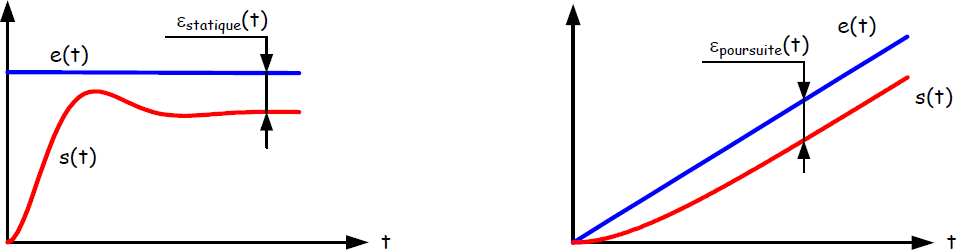
\includegraphics[width=.9\linewidth]{images/fig_erreur}
\end{center}

\subsection*{Petit développement ...}

Calculons l'écart statique pour le système précédent. On a : $\varepsilon(p)=E(p)-R(p)=E(p)-\varepsilon(p) F(p) G(p)$. En conséquences,
$\varepsilon(p)=E(p)-\varepsilon(p) F(p) G(p) 
\Longleftrightarrow \varepsilon(p)\left( 1+F(p) G(p) \right) =E(p) 
\Longleftrightarrow   \varepsilon(p) =\dfrac{E(p)}{1+F(p) G(p)}$.

\begin{resultat}
$$\varepsilon(p) =\dfrac{E(p)}{1+FTBO(p)}$$
\end{resultat}


\subsection*{Poursuivons ...}
On a $FTBO(p)=\dfrac{K_{BO}\left(1+a_1p+...+a_mp^m \right)}{p^{\alpha}\left(1+b_1p+...+b_np^n\right)}$ avec $m< n$.
\subsubsection*{FTBO de classe nulle}

\begin{itemize}
\item Pour une entrée échelon : 
$\varepsilon_{\text{permanent}}=\lim\limits_{p\to 0} p\dfrac{E_0}{p}\dfrac{1}{1+FTBO(p)} 
= \dfrac{E_0}{1+K_{BO}}$.
\item Pour une entrée de type rampe : 
$\varepsilon_{\text{permanent}}=\lim\limits_{p\to 0} p\dfrac{V}{p^2}\dfrac{1}{1+FTBO(p)} 
=+\infty$.
\item Pour une entrée de type parabole : 
$\varepsilon_{\text{permanent}}=\lim\limits_{p\to 0} p\dfrac{A}{p^3}\dfrac{1}{1+FTBO(p)} 
=+\infty$.
\end{itemize}

\subsubsection*{FTBO de classe 1}

\begin{itemize}
\item Pour une entrée échelon : 
$\varepsilon_{\text{permanent}}=\lim\limits_{p\to 0} p\dfrac{E_0}{p}\dfrac{1}{1+\dfrac{K_{BO}\left(1+a_1p+...+a_mp^m \right)}{p\left(1+b_1p+...+b_np^n\right)}} 
= 0$.
\item Pour une entrée de type rampe : 
$\varepsilon_{\text{permanent}}=\lim\limits_{p\to 0} p\dfrac{V}{p^2}\dfrac{1}{1+\dfrac{K_{BO}\left(1+a_1p+...+a_mp^m \right)}{p\left(1+b_1p+...+b_np^n\right)}} 
=\dfrac{V}{K_{BO}}$.
\item Pour une entrée de type parabole : 
$\varepsilon_{\text{permanent}}=\lim\limits_{p\to 0} p\dfrac{A}{p^3}\dfrac{1}{1+\dfrac{K_{BO}\left(1+a_1p+...+a_mp^m \right)}{p\left(1+b_1p+...+b_np^n\right)}} 
=+\infty$.
\end{itemize}

\subsubsection*{FTBO de classe 2}

\begin{itemize}
\item Pour une entrée échelon : 
$\varepsilon_{\text{permanent}}=\lim\limits_{p\to 0} p\dfrac{E_0}{p}\dfrac{1}{1+\dfrac{K_{BO}\left(1+a_1p+...+a_mp^m \right)}{p^{2}\left(1+b_1p+...+b_np^n\right)}} 
= 0$.
\item Pour une entrée de type rampe : 
$\varepsilon_{\text{permanent}}=\lim\limits_{p\to 0} p\dfrac{V}{p^2}\dfrac{1}{1+\dfrac{K_{BO}\left(1+a_1p+...+a_mp^m \right)}{p^{2}\left(1+b_1p+...+b_np^n\right)}} 
=0$.
\item Pour une entrée de type parabole : 
$\varepsilon_{\text{permanent}}=\lim\limits_{p\to 0} p\dfrac{A}{p^3}\dfrac{1}{1+\dfrac{K_{BO}\left(1+a_1p+...+a_mp^m \right)}{p^{2}\left(1+b_1p+...+b_np^n\right)}} 
=\dfrac{A}{K_{BO}}$.
\end{itemize}


\begin{resultat} ~\\

\begin{center}
\begin{tabular}{|c|c|c|c|}
\hline 
Classe & Consigne échelon & Consigne en rampe & Consigne parabolique \\
& $e(t)=E_0$ & $e(t)=V t $ & $e(t)=At^2$ \\ 
& $E(p)=\dfrac{E_0}{p}$ & $E(p)=\dfrac{V}{p^2}$ & $E(p)=\dfrac{A}{p^3}$ \\ 
\hline \hline 
&&&\\
0 & $\varepsilon_S = \dfrac{E_0}{1+K_{BO}} $ & $\varepsilon_V = +\infty$ & $\varepsilon_A = +\infty$ \\
&&&\\
\hline 
&&&\\
1 & $\varepsilon_S = 0$ & $\varepsilon_V = \dfrac{V}{K_{BO}} $ & $\varepsilon_A = +\infty$ \\
&&&\\
\hline 
&&&\\
2 & $\varepsilon_S = 0 $ & $\varepsilon_V = 0$ & $\varepsilon_A = \dfrac{A}{K_{BO}}$ \\
&&&\\
\hline 
\end{tabular}
\end{center}

\begin{rem}
L'écart statique est nul si la boucle ouverte comprend au moins une intégration. À défaut, l'augmentation du gain statique de la boucle ouverte provoque une amélioration de la précision.
\end{rem}

\end{resultat}




%\begin{methode}[Détermination de l'erreur pour un système non perturbé]
%
%\end{methode}

%\begin{methode}[Détermination de l'erreur pour un système perturbé]
%
%\end{methode}
%
%\begin{resultat}
%Tableau...
%\end{resultat}

\section{Système perturbé}
Soit le schéma-blocs suivant : 
\begin{center}
\includestandalone{images/Schema2Entrees_2F_R}
\end{center}

\vspace{.25cm}

\textbf{L'écart est caractérisé par le soustracteur principal, c'est-à-dire celui situé le plus à gauche du schéma-blocs.}

\vspace{.25cm}

Par lecture directe, on a : 
$\varepsilon(p)
=E(p)-R(p)S(p)
=E(p)-R(p)\left(H_2(p) \left(P(p)+\varepsilon(p)H_1(p) \right)\right)$
$\Longleftrightarrow 
\varepsilon(p) =E(p)- R(p)H_2(p)P(p)-R(p)H_1(p)H_2(p)\varepsilon(p) $
$\Longleftrightarrow \varepsilon(p)\left( 1+R(p)H_1(p)H_2(p)\right) =E(p)- R(p)H_2(p)P(p)$
$\Longleftrightarrow \varepsilon(p) =\dfrac{E(p)}{1+R(p)H_1(p)H_2(p)}- \dfrac{R(p)H_2(p)}{1+R(p)H_1(p)H_2(p)}P(p)$.

On a donc :
$\varepsilon(p) =\underbrace{\dfrac{1}{1+\text{FTBO}(p)} E(p)}_{\text{\'Ecart vis-à-vis de la consigne}} - \underbrace{\dfrac{R(p)H_2(p)}{1+\text{FTBO}(p)}P(p)}_{\text{\'Ecart vis-à-vis de la perturbation}}$.

Notons $H_1(p)=\dfrac{K_1}{p^\alpha_1}\dfrac{N_1(p)}{D_1(p)}$ (avec $N_1(0)=1$ et $D_1(0)=1$) et $H_2(p)=\dfrac{K_2}{p^\alpha_2}\dfrac{N_2(p)}{D_2(p)}$ (avec $N_2(0)=1$ et $D_2(0)=1$).

Par ailleurs 
$H_{\text{bo}}(p)=H_1(p)H_2(p)R(p)
=\dfrac{H_{\text{bo}}}{p^{\alpha}}\dfrac{N(p)}{D(p)}$.

On peut calculer l'écart vis-à-vis de la perturbation : 
$\varepsilon_{\text{perturbation}}
= \lim\limits_{t\to\infty}\varepsilon(t)
= \lim\limits_{p\to 0}p \varepsilon(p) 
= \lim\limits_{p\to 0} \dfrac{K_2 p^{\alpha_1+1}}{p^{\alpha_1+\alpha_2}+K_1K_2}P(p) $.

%$S(p)=H_2(p)\left(P(p)+H_1(p)\left(E(p)-R(p)S(p)\right) \right)$
%$=P(p)H_2(p)+H_1(p)H_2(p)E(p)-H_1(p)H_2(p)R(p)S(p)$ 
%$\Leftrightarrow S(p)\left( 1+H_1(p)H_2(p)R(p)\right)=P(p)H_2(p)+H_1(p)H_2(p)E(p)$
%$\Leftrightarrow S(p)=P(p)\dfrac{H_2(p)}{1+H_1(p)H_2(p)R(p)}+\dfrac{H_1(p)H_2(p)}{1+H_1(p)H_2(p)R(p)}E(p)$.

%On a donc $S(p)=P(p)\dfrac{H_2(p)}{1+\text{FTBO}(p)}+\dfrac{H_1(p)H_2(p)}{1+%\text{FTBO}(p)}E(p)$.
\begin{center}
\begin{tabular}{|c|c|c|}
\hline
Cas & Classe du système & Perturbation en échelon $P(p)=\dfrac{P_0}{p}$ \\ \hline
1 & $\alpha_1\geq 1$ & $\varepsilon_{\text{perturbation}}=0$ \\ \hline
2 & $\alpha_1=0$ et $\alpha_2=0$ & $\varepsilon_{\text{perturbation}}=\dfrac{K_2}{1+K_1K_2}P_0$ \\ \hline
3 & $\alpha_1=0$ et $\alpha_2\geq 1$ & $\varepsilon_{\text{perturbation}}=\dfrac{P_0}{K_1}$ \\ \hline
\end{tabular}
\end{center}

\begin{resultat}
Il faut au moins un intégrateur en amont d'une perturbation constante pour
annuler l'écart vis-à-vis de cette perturbation. Un intégrateur placé en aval n'a aucune
influence.

Quand ce n'est pas le cas, un gain $K_1$ important en amont de la perturbation réduit toujours
l'écart vis-à-vis de cette perturbation.
\end{resultat}


\begin{center}
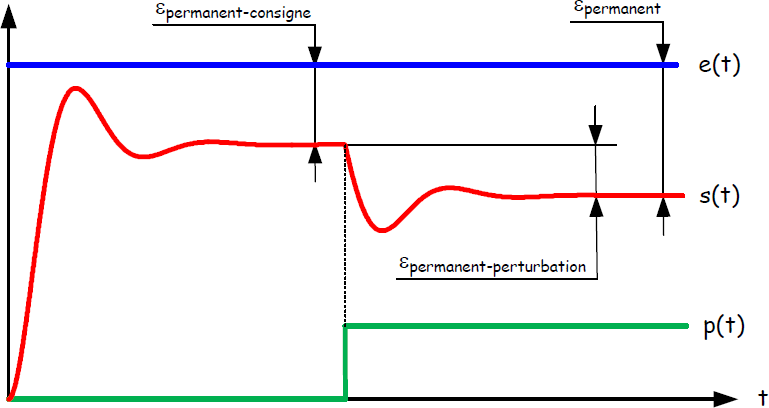
\includegraphics[width=.7\linewidth]{images/fig_erreur_02}
\end{center}


%\section{Précision et réponse fréquentielle}


\begin{thebibliography}{2}
   \bibitem[1]{ref1} Frédéric Mazet, {\it Cours d'automatique de deuxième année, Lycée Dumont Durville, Toulon.}
      \bibitem[2]{ref2} Florestan Mathurin, {\it Précision des SLCI, Lycée Bellevue, Toulouse, \url{http://florestan.mathurin.free.fr/}.}



\end{thebibliography}

\end{document}






\def\xxYongletGarde{1.1cm}
\def\xxYOnget{1.1cm}

% Activation
% Sujet
\newpage
\fichetrue \proffalse \tdtrue \coursfalse
\graphicspath{{../../style/png/}{../../Chapitre_03_Precision/Activation_AssemblageFalcon/images/}}
%%%% Paramétrage du TD %%%%
\def\xxactivite{Activation\ifprof \\ \normalsize \vspace{-.4cm}Corrigé \else \fi}
\def\xxauteur{\textsl{Xavier Pessoles}}


\def\xxnumchapitre{Chapitre 3 \vspace{.2cm}}
\def\xxchapitre{\hspace{.12cm} Précision des systèmes}

\def\xxcompetences{%
\textsl{%
\textbf{Savoirs et compétences :}\\
\vspace{-.4cm}
%\begin{itemize}[label=\ding{112},font=\color{ocre}] 
%%\item \textit{Mod3.C2 : } pôles dominants et réduction de l’ordre du modèle : principe, justification
%%\item \textit{Res2.C4 : } stabilité des SLCI : définition entrée bornée -- sortie bornée (EB -- SB)	
%%\item \textit{Res2.C5 : } stabilité des SLCI : équation caractéristique	
%\item \textit{Res2.C6 : } stabilité des SLCI : position des pôles dans le plan complexe
%\item \textit{Res2.C7 : } stabilité des SLCI : marges de stabilité (de gain et de phase)
%\end{itemize}
}}


\def\xxfigures{
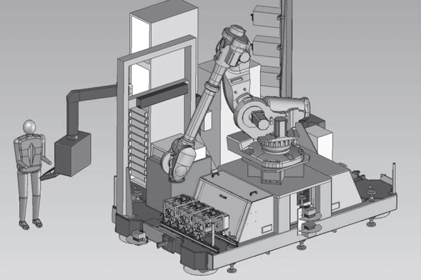
\includegraphics[width=.7\textwidth]{image1}
}%figues de la page de garde

\def\xxtitreexo{Cellule d'assemblage pour avion Falcon}
\def\xxsourceexo{D'après concours E3A -- PSI 2015.}



\iflivret
\pagestyle{empty}


%%%%%%%% PAGE DE GARDE COURS
\ifcours
\begin{tikzpicture}[remember picture,overlay]
\node at (current page.north west)
{\begin{tikzpicture}[remember picture,overlay]
\node[anchor=north west,inner sep=0pt] at (0,0) {\includegraphics[width=\paperwidth]{\thechapterimage}};
\draw[anchor=west] (-2cm,-8cm) node [line width=2pt,rounded corners=15pt,draw=ocre,fill=white,fill opacity=0.6,inner sep=40pt]{\strut\makebox[22cm]{}};
\draw[anchor=west] (1cm,-8cm) node {\huge\sffamily\bfseries\color{black} %
\begin{minipage}{1cm}
\rotatebox{90}{\LARGE\sffamily\textsc{\color{ocre}\textbf{\xxnumpartie}}}
\end{minipage} \hfill
\begin{minipage}[c]{14cm}
\begin{titrepartie}
\begin{flushright}
\renewcommand{\baselinestretch}{1.1} 
\Large\sffamily\textsc{\textbf{\xxpartie}}
\renewcommand{\baselinestretch}{1} 
\end{flushright}
\end{titrepartie}
\end{minipage} \hfill
\begin{minipage}[c]{3.5cm}
{\large\sffamily\textsc{\textbf{\color{ocre} \discipline}}}
\end{minipage} 
 };
\end{tikzpicture}};
\end{tikzpicture}


\begin{tikzpicture}[overlay]
\node[shape=rectangle, 
      rounded corners = .25 cm,
	  draw= ocre,
	  line width=2pt, 
	  fill = ocre!10,
	  minimum width  = 2.5cm,
	  minimum height = 3cm,] at (18cm,0) {};
\node at (17.7cm,0) {\rotatebox{90}{\textbf{\Large\color{ocre}{\classe}}}};
%{};
\end{tikzpicture}

\vspace{3.5cm}

\begin{tikzpicture}[remember picture,overlay]
\draw[anchor=west] (-2cm,-6cm) node {\huge\sffamily\bfseries\color{black} %
\begin{minipage}{2cm}
\begin{center}
\LARGE\sffamily\textsc{\color{ocre}\textbf{\xxactivite}}
\end{center}
\end{minipage} \hfill
\begin{minipage}[c]{15cm}
\begin{titrechapitre}
\renewcommand{\baselinestretch}{1.1} 
\Large\sffamily\textsc{\textbf{\xxnumchapitre}}

\Large\sffamily\textsc{\textbf{\xxchapitre}}
\vspace{.5cm}

\renewcommand{\baselinestretch}{1} 
\normalsize\normalfont
\xxcompetences
\end{titrechapitre}
\end{minipage}  };
\end{tikzpicture}
\vfill

\begin{flushright}
\begin{minipage}[c]{.3\linewidth}
\begin{center}
\xxfigures
\end{center}
\end{minipage}\hfill
\begin{minipage}[c]{.6\linewidth}
\startcontents
\printcontents{}{1}{}
\end{minipage}
\end{flushright}

\begin{tikzpicture}[remember picture,overlay]
\draw[anchor=west] (4.5cm,-.7cm) node {
\begin{minipage}[c]{.2\linewidth}
\begin{flushright}

\includegraphics[width=2cm]{logoCC}
\end{flushright}
\end{minipage}
\begin{minipage}[c]{.2\linewidth}
\textsl{\xxauteur} \\
\textsl{\classe}
\end{minipage}
 };
\end{tikzpicture}
\newpage
\pagestyle{fancy}

\newpage
\pagestyle{fancy}

\else
\fi


%%%%%%%% PAGE DE GARDE TD
\iftd
%\begin{tikzpicture}[remember picture,overlay]
%\node at (current page.north west)
%{\begin{tikzpicture}[remember picture,overlay]
%\draw[anchor=west] (-2cm,-3.25cm) node [line width=2pt,rounded corners=15pt,draw=ocre,fill=white,fill opacity=0.6,inner sep=40pt]{\strut\makebox[22cm]{}};
%\draw[anchor=west] (1cm,-3.25cm) node {\huge\sffamily\bfseries\color{black} %
%\begin{minipage}{1cm}
%\rotatebox{90}{\LARGE\sffamily\textsc{\color{ocre}\textbf{\xxnumpartie}}}
%\end{minipage} \hfill
%\begin{minipage}[c]{13.5cm}
%\begin{titrepartie}
%\begin{flushright}
%\renewcommand{\baselinestretch}{1.1} 
%\Large\sffamily\textsc{\textbf{\xxpartie}}
%\renewcommand{\baselinestretch}{1} 
%\end{flushright}
%\end{titrepartie}
%\end{minipage} \hfill
%\begin{minipage}[c]{3.5cm}
%{\large\sffamily\textsc{\textbf{\color{ocre} \discipline}}}
%\end{minipage} 
% };
%\end{tikzpicture}};
%\end{tikzpicture}

%%%%%%%%%% PAGE DE GARDE TD %%%%%%%%%%%%%%%
%\begin{tikzpicture}[overlay]
%\node[shape=rectangle, 
%      rounded corners = .25 cm,
%	  draw= ocre,
%	  line width=2pt, 
%	  fill = ocre!10,
%	  minimum width  = 2.5cm,
%	  minimum height = 2.5cm,] at (18.5cm,0) {};
%\node at (17.7cm,0) {\rotatebox{90}{\textbf{\Large\color{ocre}{\classe}}}};
%%{};
%\end{tikzpicture}

% PARTIE ET CHAPITRE
%\begin{tikzpicture}[remember picture,overlay]
%\draw[anchor=west] (-1cm,-2.1cm) node {\large\sffamily\bfseries\color{black} %
%\begin{minipage}[c]{15cm}
%\begin{flushleft}
%\xxnumchapitre \\
%\xxchapitre
%\end{flushleft}
%\end{minipage}  };
%\end{tikzpicture}

% Bandeau titre exo
\begin{tikzpicture}[remember picture,overlay]
\draw[anchor=west] (-2cm,-4cm) node {\huge\sffamily\bfseries\color{black} %
\begin{minipage}{5cm}
\begin{center}
\LARGE\sffamily\color{ocre}\textbf{\textsc{\xxactivite}}

\begin{center}
\xxfigures
\end{center}

\end{center}
\end{minipage} \hfill
\begin{minipage}[c]{12cm}
\begin{titrechapitre}
\renewcommand{\baselinestretch}{1.1} 
\large\sffamily\textbf{\textsc{\xxtitreexo}}

\small\sffamily{\textbf{\textit{\color{black!70}\xxsourceexo}}}
\vspace{.5cm}

\renewcommand{\baselinestretch}{1} 
\normalsize\normalfont
\xxcompetences
\end{titrechapitre}
\end{minipage}  };
\end{tikzpicture}

\else
\fi


%%%%%%%% PAGE DE GARDE FICHE
\iffiche
\begin{tikzpicture}[remember picture,overlay]
\node at (current page.north west)
{\begin{tikzpicture}[remember picture,overlay]
\draw[anchor=west] (-2cm,-3.25cm) node [line width=2pt,rounded corners=15pt,draw=ocre,fill=white,fill opacity=0.6,inner sep=40pt]{\strut\makebox[22cm]{}};
\draw[anchor=west] (1cm,-3.25cm) node {\huge\sffamily\bfseries\color{black} %
\begin{minipage}{1cm}
\rotatebox{90}{\LARGE\sffamily\textsc{\color{ocre}\textbf{\xxnumpartie}}}
\end{minipage} \hfill
\begin{minipage}[c]{14cm}
\begin{titrepartie}
\begin{flushright}
\renewcommand{\baselinestretch}{1.1} 
\large\sffamily\textsc{\textbf{\xxpartie} \\} 

\vspace{.2cm}

\normalsize\sffamily\textsc{\textbf{\xxnumchapitre -- \xxchapitre}}
\renewcommand{\baselinestretch}{1} 
\end{flushright}
\end{titrepartie}
\end{minipage} \hfill
\begin{minipage}[c]{3.5cm}
{\large\sffamily\textsc{\textbf{\color{ocre} \discipline}}}
\end{minipage} 
 };
\end{tikzpicture}};
\end{tikzpicture}


\begin{tikzpicture}[overlay]
\node[shape=rectangle, 
      rounded corners = .25 cm,
	  draw= ocre,
	  line width=2pt, 
	  fill = ocre!10,
	  minimum width  = 2.5cm,
	  minimum height = 2.5cm,] at (18.5cm,0.5cm) {};
%	  minimum height = 2.5cm,] at (18.5cm,0cm) {};
\node at (17.7cm,0.5) {\rotatebox{90}{\textsf{\textbf{\large\color{ocre}{\classe}}}}};
%{};
\end{tikzpicture}



\else
\fi



\else
\pagestyle{empty}


%%%%%%%% PAGE DE GARDE COURS
\ifcours
\begin{tikzpicture}[remember picture,overlay]
\node at (current page.north west)
{\begin{tikzpicture}[remember picture,overlay]
\node[anchor=north west,inner sep=0pt] at (0,0) {\includegraphics[width=\paperwidth]{\thechapterimage}};
\draw[anchor=west] (-2cm,-8cm) node [line width=2pt,rounded corners=15pt,draw=ocre,fill=white,fill opacity=0.6,inner sep=40pt]{\strut\makebox[22cm]{}};
\draw[anchor=west] (1cm,-8cm) node {\huge\sffamily\bfseries\color{black} %
\begin{minipage}{1cm}
\rotatebox{90}{\LARGE\sffamily\textsc{\color{ocre}\textbf{\xxnumpartie}}}
\end{minipage} \hfill
\begin{minipage}[c]{14cm}
\begin{titrepartie}
\begin{flushright}
\renewcommand{\baselinestretch}{1.1} 
\Large\sffamily\textsc{\textbf{\xxpartie}}
\renewcommand{\baselinestretch}{1} 
\end{flushright}
\end{titrepartie}
\end{minipage} \hfill
\begin{minipage}[c]{3.5cm}
{\large\sffamily\textsc{\textbf{\color{ocre} \discipline}}}
\end{minipage} 
 };
\end{tikzpicture}};
\end{tikzpicture}


\begin{tikzpicture}[overlay]
\node[shape=rectangle, 
      rounded corners = .25 cm,
	  draw= ocre,
	  line width=2pt, 
	  fill = ocre!10,
	  minimum width  = 2.5cm,
	  minimum height = 3cm,] at (18cm,0) {};
\node at (17.7cm,0) {\rotatebox{90}{\textbf{\Large\color{ocre}{\classe}}}};
%{};
\end{tikzpicture}

\vspace{3.5cm}

\begin{tikzpicture}[remember picture,overlay]
\draw[anchor=west] (-2cm,-6cm) node {\huge\sffamily\bfseries\color{black} %
\begin{minipage}{2cm}
\begin{center}
\LARGE\sffamily\textsc{\color{ocre}\textbf{\xxactivite}}
\end{center}
\end{minipage} \hfill
\begin{minipage}[c]{15cm}
\begin{titrechapitre}
\renewcommand{\baselinestretch}{1.1} 
\Large\sffamily\textsc{\textbf{\xxnumchapitre}}

\Large\sffamily\textsc{\textbf{\xxchapitre}}
\vspace{.5cm}

\renewcommand{\baselinestretch}{1} 
\normalsize\normalfont
\xxcompetences
\end{titrechapitre}
\end{minipage}  };
\end{tikzpicture}
\vfill

\begin{flushright}
\begin{minipage}[c]{.3\linewidth}
\begin{center}
\xxfigures
\end{center}
\end{minipage}\hfill
\begin{minipage}[c]{.6\linewidth}
\startcontents
\printcontents{}{1}{}
\end{minipage}
\end{flushright}

\begin{tikzpicture}[remember picture,overlay]
\draw[anchor=west] (4.5cm,-.7cm) node {
\begin{minipage}[c]{.2\linewidth}
\begin{flushright}

\includegraphics[width=2cm]{logoCC}
\end{flushright}
\end{minipage}
\begin{minipage}[c]{.2\linewidth}
\textsl{\xxauteur} \\
\textsl{\classe}
\end{minipage}
 };
\end{tikzpicture}
\newpage
\pagestyle{fancy}

\newpage
\pagestyle{fancy}

\else
\fi


%%%%%%%% PAGE DE GARDE TD
\iftd
%\begin{tikzpicture}[remember picture,overlay]
%\node at (current page.north west)
%{\begin{tikzpicture}[remember picture,overlay]
%\draw[anchor=west] (-2cm,-3.25cm) node [line width=2pt,rounded corners=15pt,draw=ocre,fill=white,fill opacity=0.6,inner sep=40pt]{\strut\makebox[22cm]{}};
%\draw[anchor=west] (1cm,-3.25cm) node {\huge\sffamily\bfseries\color{black} %
%\begin{minipage}{1cm}
%\rotatebox{90}{\LARGE\sffamily\textsc{\color{ocre}\textbf{\xxnumpartie}}}
%\end{minipage} \hfill
%\begin{minipage}[c]{13.5cm}
%\begin{titrepartie}
%\begin{flushright}
%\renewcommand{\baselinestretch}{1.1} 
%\Large\sffamily\textsc{\textbf{\xxpartie}}
%\renewcommand{\baselinestretch}{1} 
%\end{flushright}
%\end{titrepartie}
%\end{minipage} \hfill
%\begin{minipage}[c]{3.5cm}
%{\large\sffamily\textsc{\textbf{\color{ocre} \discipline}}}
%\end{minipage} 
% };
%\end{tikzpicture}};
%\end{tikzpicture}

%%%%%%%%%% PAGE DE GARDE TD %%%%%%%%%%%%%%%
%\begin{tikzpicture}[overlay]
%\node[shape=rectangle, 
%      rounded corners = .25 cm,
%	  draw= ocre,
%	  line width=2pt, 
%	  fill = ocre!10,
%	  minimum width  = 2.5cm,
%	  minimum height = 2.5cm,] at (18.5cm,0) {};
%\node at (17.7cm,0) {\rotatebox{90}{\textbf{\Large\color{ocre}{\classe}}}};
%%{};
%\end{tikzpicture}

% PARTIE ET CHAPITRE
%\begin{tikzpicture}[remember picture,overlay]
%\draw[anchor=west] (-1cm,-2.1cm) node {\large\sffamily\bfseries\color{black} %
%\begin{minipage}[c]{15cm}
%\begin{flushleft}
%\xxnumchapitre \\
%\xxchapitre
%\end{flushleft}
%\end{minipage}  };
%\end{tikzpicture}

% Bandeau titre exo
\begin{tikzpicture}[remember picture,overlay]
\draw[anchor=west] (-2cm,-4cm) node {\huge\sffamily\bfseries\color{black} %
\begin{minipage}{5cm}
\begin{center}
\LARGE\sffamily\color{ocre}\textbf{\textsc{\xxactivite}}

\begin{center}
\xxfigures
\end{center}

\end{center}
\end{minipage} \hfill
\begin{minipage}[c]{12cm}
\begin{titrechapitre}
\renewcommand{\baselinestretch}{1.1} 
\large\sffamily\textbf{\textsc{\xxtitreexo}}

\small\sffamily{\textbf{\textit{\color{black!70}\xxsourceexo}}}
\vspace{.5cm}

\renewcommand{\baselinestretch}{1} 
\normalsize\normalfont
\xxcompetences
\end{titrechapitre}
\end{minipage}  };
\end{tikzpicture}

\else
\fi


%%%%%%%% PAGE DE GARDE FICHE
\iffiche
\begin{tikzpicture}[remember picture,overlay]
\node at (current page.north west)
{\begin{tikzpicture}[remember picture,overlay]
\draw[anchor=west] (-2cm,-3.25cm) node [line width=2pt,rounded corners=15pt,draw=ocre,fill=white,fill opacity=0.6,inner sep=40pt]{\strut\makebox[22cm]{}};
\draw[anchor=west] (1cm,-3.25cm) node {\huge\sffamily\bfseries\color{black} %
\begin{minipage}{1cm}
\rotatebox{90}{\LARGE\sffamily\textsc{\color{ocre}\textbf{\xxnumpartie}}}
\end{minipage} \hfill
\begin{minipage}[c]{14cm}
\begin{titrepartie}
\begin{flushright}
\renewcommand{\baselinestretch}{1.1} 
\large\sffamily\textsc{\textbf{\xxpartie} \\} 

\vspace{.2cm}

\normalsize\sffamily\textsc{\textbf{\xxnumchapitre -- \xxchapitre}}
\renewcommand{\baselinestretch}{1} 
\end{flushright}
\end{titrepartie}
\end{minipage} \hfill
\begin{minipage}[c]{3.5cm}
{\large\sffamily\textsc{\textbf{\color{ocre} \discipline}}}
\end{minipage} 
 };
\end{tikzpicture}};
\end{tikzpicture}


\begin{tikzpicture}[overlay]
\node[shape=rectangle, 
      rounded corners = .25 cm,
	  draw= ocre,
	  line width=2pt, 
	  fill = ocre!10,
	  minimum width  = 2.5cm,
	  minimum height = 2.5cm,] at (18.5cm,0.5cm) {};
%	  minimum height = 2.5cm,] at (18.5cm,0cm) {};
\node at (17.7cm,0.5) {\rotatebox{90}{\textsf{\textbf{\large\color{ocre}{\classe}}}}};
%{};
\end{tikzpicture}



\else
\fi



\fi
\setlength{\columnseprule}{.1pt}

\pagestyle{fancy}
\thispagestyle{plain}


\vspace{4.5cm}

\def\columnseprulecolor{\color{ocre}}
\setlength{\columnseprule}{0.4pt} 

%%%%%%%%%%%%%%%%%%%%%%%


\begin{multicols}{2}
\setcounter{exo}{0}
\subsection*{Présentation}
Le tronçon central du fuselage du Falcon 7X est assemblé par rivetage grâce à un robot 6 axes. Les rivets sont stockés dans des cassettes rangées verticalement. Un chariot de sélection se déplace verticalement pour déplacer une buse d'aspiration qui permettra d'acheminer les rivets contenus dans la cassette vers l'effecteur (robot). Le chariot fait l'objet de cette étude.

\begin{center}
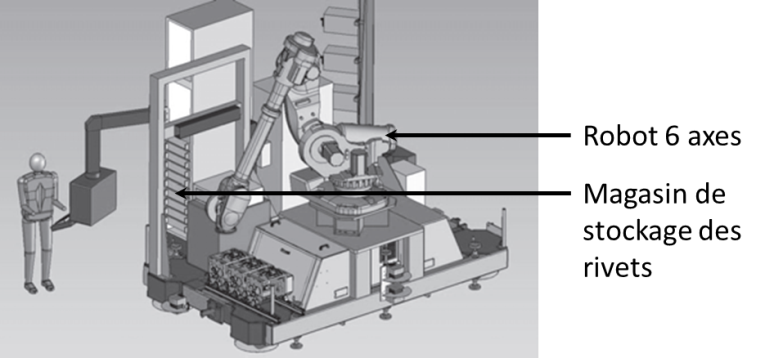
\includegraphics[width=7cm]{image5}
\end{center} 

\begin{obj}
Vérifier que les correcteurs proposés permettent ou non d'obtenir un écart statique nul et un écart en vitesse nul.
\end{obj}
% 
%L'objectif de cette partie est de valider les choix effectués par la société pour le sous ensemble de sélection des fixations de la cellule (exigence 1.1).

%\vfill
%
%\begin{center}
%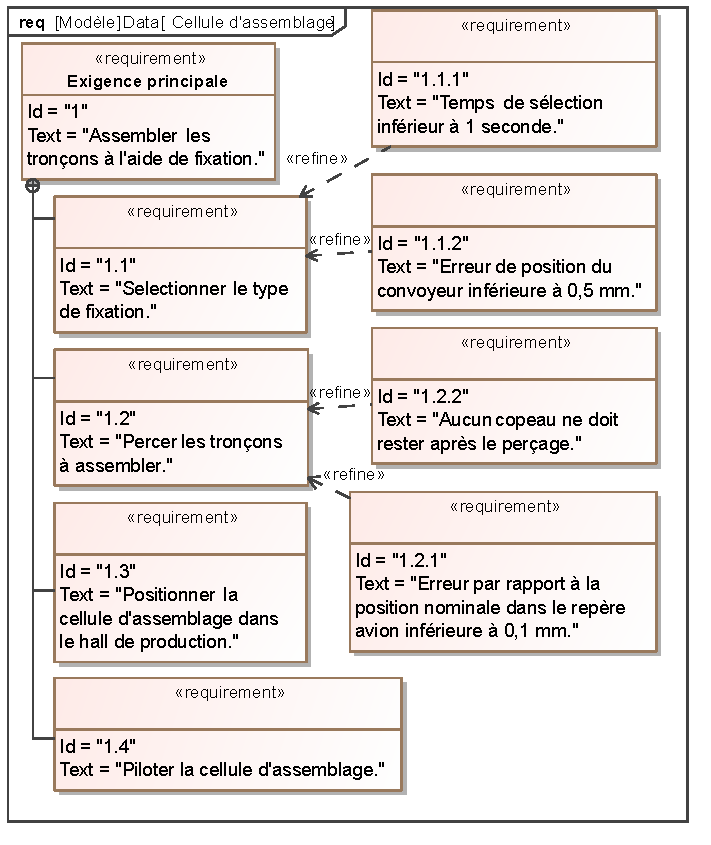
\includegraphics[width=7cm]{Exigences}
%\end{center} 




% 
%\subsection*{Axe chariot}
%Le déplacement du chariot est assuré par un axe numérique asservi en vitesse et en position. Cet axe est composé d'un moteur à courant continu, d'un système de transmission de puissance de type poulies / courroie et d'un rail.
% 
%\begin{center}
%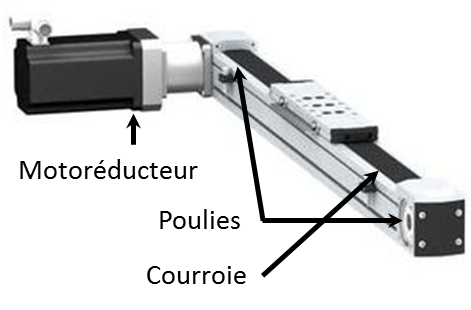
\includegraphics[width=4.5cm]{image7}
%\end{center} 
%
%
%\subsection*{Modélisation du système de déplacement du chariot}
%
%\begin{center}
%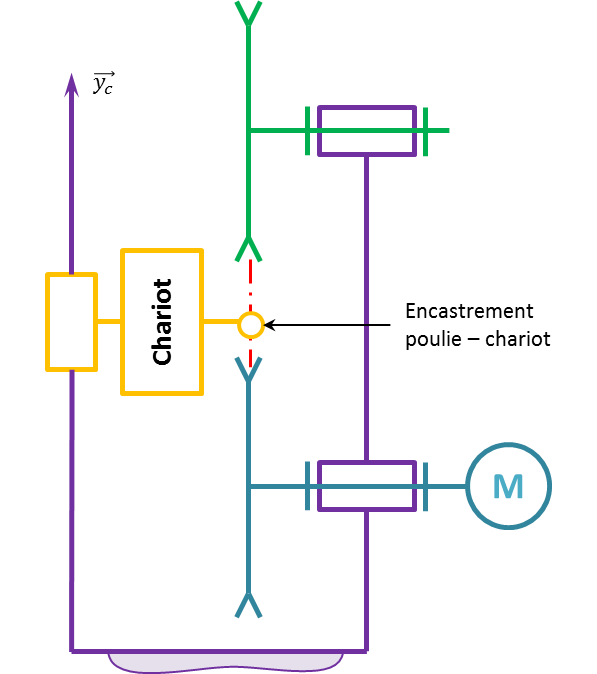
\includegraphics[width=5cm]{image8}
%\end{center} 
%
%
%\fi

%
%
%
%\section*{Sélectionner les fixations – Exigence 1.1}
%\ifprof
%\else 
%Afin de sélectionner le type de fixation, la buse d'aspiration doit être déplacée en face de la cassette avec une erreur inférieure à $\SI{0,5}{mm}$ (voir exigences fonctionnelles). Cependant le fabricant du système poulie-courroie du rail indique déjà une erreur de $\pm \SI{0,25}{mm}$ due notamment à l'élasticité de la courroie. Par conséquent, l'erreur en position de la commande doit être nulle. De plus, afin de ne pas perdre de temps lors de la production, le temps maximal de déplacement lors de la sélection est imposé à une seconde.
%
%L'étude se fera dans le cas le plus défavorable c'est-à-dire un déplacement du chariot vers le haut entre les deux cassettes de rivets les plus éloignées. L'axe de déplacement est appelé $\vect{y_c}$
%\subsection*{Notations domaine temporel – domaine de Laplace}
%
%Les notations entre le domaine temporel et celui de Laplace sont données dans la suite. Ainsi, si la fonction $f(t)$ possède une transformée de Laplace, elle sera notée : $F(p) = \mathcal{L}[f(t)]$.
%Les équations caractéristiques du moteur à courant continu sont rappelées ci-dessous (les conditions de Heaviside sont respectées) :
%\begin{itemize}[label=\ding{112},font=\color{ocre}] 
%\item $u(t)=e(t)+L \dfrac{di(t)}{\text{d} t}+Ri(t)$;
%\item $e(t)=K_E \omega_m (t)$ ;
%\item $C_M (t)=K_C i(t)$ ;
%\item $J_{eq}  \dfrac{d\omega_m)}{\text{d} t}+f\omega_m (t)=C_M (t)-C_R (t)$.
%\end{itemize}
%
%Avec : 
%\begin{itemize}[label=\ding{112},font=\color{ocre}] 
%\item $u(t)$ : tension moteur ;
%\item $i(t)$ : courant moteur ; 
%\item $e(t)$ : force contre-électromotrice ;
%\item $\omega_m(t)$ : vitesse de rotation moteur ;
%\item $C_M (t)$ : couple moteur ;
%\item $C_R (t)$: couple résistant modélisant l'action de pesanteur.
%\end{itemize}
%\fi
%
%\subsection*{Critères à respecter pour l'exigence 1.2}
%\ifprof
%\else
%\footnotesize{
%\begin{center}
%\begin{tabular}{|p{2cm}|p{2.5cm}|p{2cm}|}
%\hline
%Exigence	& Critères & Niveaux \\ \hline
%Déplacer le chariot	& Précision :
%erreur statique par rapport à une consigne de vitesse constante	
%& NULLE \\ \hline
%	& Rapidité : temps de réponse à 5\% en réponse à une consigne échelon 
%	& $Tr_{5\%} = \SI{0,1}{s}$  maxi \\ \hline
%	& Stabilité : & \\
%	& Marge de gain & \SI{6}{dB} mini \\
%	&Marge de gain & $\ang{45}$ mini \\
%\hline
%\end{tabular}
%\end{center}}

%\fi
%\subsection*{Choix d'une architecture de la chaine de transmission}
%\subparagraph{}
%\textit{Proposer sous la forme d'un schéma une autre solution permettant le déplacement du chariot. La conversion de l'énergie électrique en énergie mécanique par un moteur doit être conservée.}
%
%\ifprof
%\begin{corrige}
%Utilisation d’un système vis-écrou.
%\end{corrige}
%\else
%\fi
%
%\ifprof
%\else
%Compte tenu des vitesses de translation importantes, le système retenu est de type poulie-courroie.
%\fi
%
%\subsection*{Détermination de l'inertie équivalente} 
%\ifprof
%\else
%
%Les grandeurs caractéristiques (notations et valeurs) des éléments de l'axe du chariot sont données dans le tableau ci-dessous :
%\begin{center}
%\begin{tabular}{|p{3cm}|c|c|}
%\hline
%Moment d'inertie du rotor du moteur autour de son axe&	$J_m$ & $\num{140d-6}\si{kg.m^2}$ \\ \hline
%Moment d'inertie du réducteur ramené à l'arbre moteur&	$J_{réd}$ & $\num{60d-4}\si{kg.m^2}$ \\ \hline
%Moment d'inertie de la poulie motrice autour de son axe&	$J_{PM}$	&$ \num{38d-4}\si{kg.m^2}$ \\ \hline
%Moment d'inertie de la poulie réceptrice autour de son axe&	$J_{PR}$ & $\num{38d-4}\si{kg.m^2}$ \\ \hline
%Masse totale du chariot	&$M$ &$\SI{5}{kg}$ \\ \hline
%Vitesse de rotation de l'arbre moteur &$\omega_m$ &  \\ \hline
%Vitesse de rotation de l'arbre de sortie du réducteur	&$\omega_r$&  \\ \hline
%Rayon d'une poulie motrice ou réceptrice	& $R_P$ &$\SI{45}{mm}$ \\ \hline
%Rapport de réduction réducteur ($\omega_r/\omega_m$)	& $\lambda$	&$1/5$ \\ \hline
%\end{tabular}
%\end{center}
%\fi
%
%\subparagraph{}
%\textit{À partir des grandeurs définies déterminer l'expression littérale de l'inertie équivalente $J_{eq}$ de l'ensemble $\Sigma=$\{moteur+réducteur+poulies+chariot\} ramenée sur l'arbre moteur. Cette inertie équivalente est définie par $E_c (\Sigma)=1/2 J_{eq} \omega_m^2$.}
%\ifprof
%\begin{corrige}
%$\mathcal{E}_c(\Sigma)=\mathcal{E}_c (\text{moteur})+\mathcal{E}_c (\text{réducteur})+\mathcal{E}_c (\text{poulies})+\mathcal{E}_c (\text{chariot})$.
%\begin{itemize}
%	\item $\mathcal{E}_c (\text{moteur})=1/2 J_m \omega_m^2$;
%	\item $\mathcal{E}_c (\text{réducteur})=1/2 J_{\text{red}} \omega_m^2$;
%	\item $\mathcal{E}_c (\text{poulies})=1/2 (J_{\text{Pm}}+J_{\text{PR}}  ) \omega_{\text{red}}^2=1/2 (J_{\text{Pm}}+J_{\text{PR}}  ) \lambda^2 \omega_m^2$;
%	\item $\mathcal{E}_c (\text{chariot})=1/2 MV^2=1/2 MR_p^2 \lambda^2 \omega_m^2$.
%\end{itemize}
%On a donc $J_{\text{eq}}=MR_p^2 \lambda^2+(J_{\text{Pm}}+J_{\text{PR}}  ) \lambda^2+J_{\text{red}}+J_m$.
%
%\end{corrige}
%\else
%\fi
%
%\subparagraph{}
%\textit{Déterminer la valeur numérique de l'expression précédente.}
%\ifprof
%\begin{corrige}
%$J_{eq}=\SI{0,0068}{kg.m^2}$
%\end{corrige}
%\else
%\fi
%
%\subsection*{Modèle de connaissance du moteur à courant continu}
%
%\begin{obj}
%L'objectif de cette partie est d'établir un modèle de la motorisation de l'axe afin de simuler un déplacement.
%\end{obj}
%
%\subparagraph{}
%\textit{À partir des équations du moteur à courant continu, réaliser le schéma bloc du moteur à courant continu.}
%\ifprof
%\begin{corrige} ~\\
%
%\begin{center}
%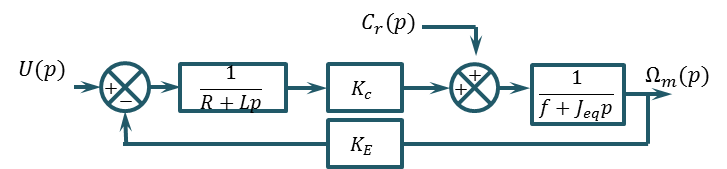
\includegraphics[width=7cm]{corr_01}
%\end{center} 
%\end{corrige}
%\else
%\fi
%
%\subparagraph{}
%\textit{En considérant que $C_R (p)=0$, déterminer la fonction de transfert $H_M (p)=\dfrac{\Omega_m (p)}{U(p)}$ sous sa forme canonique.}
%\ifprof
%\begin{corrige}
%$H_m (p)=\dfrac{\dfrac{K_C}{K_c K_E+Rf}}{1+\dfrac{RJ_eq+Lf}{K_c K_E+Rf}p+\dfrac{LJ_eq}{K_c K_E+Rf} p^2}$
%\end{corrige}
%\else
%\fi
%
%\subparagraph{}
%\textit{Montrer que la fonction de transfert $H_M (p)$ peut se mettre sous la forme $H_M (p)=\dfrac{K_C}{K_C K_e+RJ_{eq} p+LJ_{eq} p^2 }$. Justifier la réponse. Pour cette question, la valeur numérique de $J_{eq}$ considérée sera $J_{eq}=\num{7d-3}\si{kg.m^2}$ indépendamment du résultat numérique calculé précédemment.}
%\ifprof
%\begin{corrige}
%En faisant les applications numériques on montre que $Rf$ est négligeable devant $K_c K_E$ et que $Lf$ et négligeable devant $RJ_{eq}$. On a donc : 
%$H_m (p)=\dfrac{\dfrac{K_C}{K_c K_E}}{1+\dfrac{RJ_{eq}}{K_c K_E }p+\dfrac{LJ_{eq}}{K_c K_E }p^2 }=\dfrac{K_C}{K_c K_E+RJ_{eq} p+LJ_{eq} p^2 }$.
%
%\end{corrige}
%\else
%\fi
%
%\subparagraph{}
%\textit{Montrer qu'avec l'expression, $H_M (p)$ peut s'écrire sous la forme $H_M (p)=\dfrac{K_M}{(1+T_E p)(1+T_M p)}$  avec $T_E<T_M$.}
%\ifprof
%\begin{corrige}
%$
%\left\{
%\begin{array}{l}
%T_e+T_m= \dfrac{RJ_{eq}}{K_c K_e}\\
%T_e T_m=\dfrac{LJ_{eq}}{K_C K_e}
%\end{array}
%\right.
%$
%On a (résolution d’une équation du second degré):
%
%$Te=\dfrac{\dfrac{RJ_{eq}}{K_c K_e}-\sqrt{\left(\dfrac{RJ_{eq}}{K_c K_e}\right)^2 - 4\dfrac{LJ_{eq}}{K_c K_e}}}{2}$. $T_e=\SI{0,0051}{s}$ et $T_m=\SI{0,0074}{s}$.
%
%
%\end{corrige}
%\else
%\fi
%\section*{Étude de l'asservissement en position de l'axe}
%\subsection*{Modélisation de l'asservissement en position}
%\ifprof
%\else
%
%
%La partie précédente a permis de déterminer un modèle du moteur. La suite de l'étude va permettre, par simulation, de déterminer les réglages nécessaires de l'axe vis-à-vis du cahier des charges. La figure suivante présente le principe de l'asservissement de l'axe du chariot.
% 
%\begin{center}
%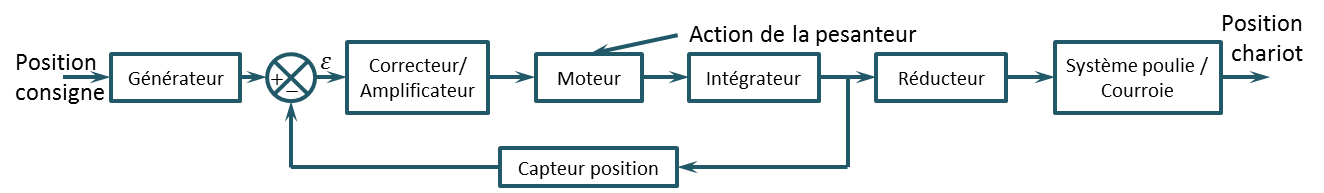
\includegraphics[width=7cm]{image9}
%\end{center} 
%
%Les grandeurs caractéristiques des blocs de l'asservissement de l'axe chariot sont données dans le tableau ci-dessous :
%\begin{center}
%\begin{tabular}{|c|c|c|}
%\hline
%Générateur & $K_G$ & À déterminer \\
%\hline
%Capteur de position	& $K_\text{capt}$ & $\num{5d-3}\si{V.rad^(-1)}$ \\
%\hline
%Correcteur amplificateur	 & $C(p)$ & Variable \\
%\hline
%\end{tabular}
%\end{center}
%\fi
%
%\subparagraph{}
%\textit{Quelle doit être la valeur de $K_G$ pour assurer un asservissement correct (c'est-à-dire l'écart $\varepsilon$ doit être nul si la position de l'axe est identique à la consigne) ?}
%\ifprof
%\begin{corrige} ~\\
%
%On doit avoir $K_G=K_{\text{capt}} \dfrac{1}{\lambda} \dfrac{1}{R_p}=\SI{0,556}{V.rad^{-1}.m^{-1}}$.
%\end{corrige}
%\else
%\fi
%
%\subparagraph{}
%\textit{Donner le schéma-blocs de l'asservissement.}
%\ifprof
%\begin{corrige} ~\\
%
%\begin{center}
%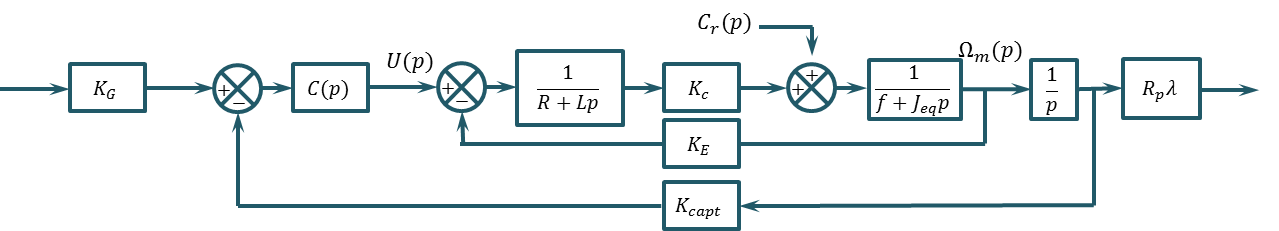
\includegraphics[width=7cm]{corr_02}
%\end{center} 
%
%\end{corrige}
%\else
%\fi

\subsection*{Étude du modèle simplifié}
\ifprof
\else
Afin de faciliter les calculs, le schéma bloc à retour unitaire est donné figure suivante. Le couple résistant $C_r$ dû à l'action de pesanteur est supposé constant.
 
 \begin{center}
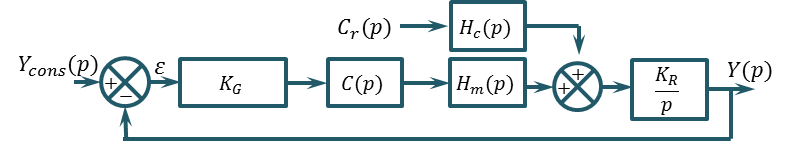
\includegraphics[width=\linewidth]{image10}
\end{center} 


Avec : 

\noindent $H_M (p)=\dfrac{K_M}{(1+T_E p)(1+T_M p)} \text{ et }
H_C (p)=\dfrac{\dfrac{\left(R+Lp\right)K_M}{K_C}}{(1+T_E p)(1+T_M p)}$.
%\item $C_R (p)=C_r/p$;
%\item $K_R=R_p \lambda$.
%\end{itemize}
\fi

\subparagraph{}
\textit{Donner l'expression de $\varepsilon(p)$.}
\ifprof
\begin{corrige}~\\
On raisonne par superposition :

Si $C_r (p)=0$: 

$$Y_1 (p)
=Y_{\text{cons}}(p) \dfrac{\dfrac{K_G K_{\text{Capt}} C(p) H_m (p) K_r}{p}}{1+\dfrac{K_G K_{\text{Capt}} C(p) H_m (p) K_r}{p}}$$

$$
=Y_{\text{cons}} (p) \dfrac{K_G K_{\text{Capt}} C(p) H_m (p) K_r}{p+K_G K_{\text{Capt}} C(p) H_m (p) K_r } 
$$

$$
=Y_{\text{cons}} (p) \dfrac{K_G K_{\text{Capt}} C(p) K_M  K_r}{(1+T_E p)(1+T_M p)p+K_G K_{\text{Capt}} C(p) K_M K_r )}$$.

\end{corrige}

\begin{corrige}
Si $Y_{\text{Cons}} (p)=0$ :

$$Y_2 (p)
=C_r (p) \dfrac{\dfrac{H_c (p) K_r}{p}}{1+\dfrac{K_r K_G K_{\text{Capt}} C(p) H_m (p)}{p} }$$

$$
=C_r (p) \dfrac{H_c (p) K_r}{p+K_r K_G K_{\text{Capt}} C(p) H_m (p) }$$
$$
=C_r (p) \dfrac{\dfrac{(R+Lp) K_M  K_r}{K_C }}{(1+T_E p)(1+T_M p)p+K_r K_G K_{\text{Capt}} C(p) K_M }$$

On a donc :
$Y(p)=Y_1 (p)+Y_2 (p)$.

\end{corrige}
\else
\fi

\subparagraph{}
\textit{On souhaite déterminer l'erreur en position du système. Calculer l'écart statique pour $C(p)=K_p$. Pouvait-on prévoir le résultat ?}
\ifprof
\begin{corrige}
\end{corrige}
\else
\fi


\subparagraph{}
\textit{On souhaite déterminer l'erreur en position du système. Calculer l'écart statique pour $C(p)=\dfrac{K_i}{p}$. Pouvait-on prévoir le résultat ?}
\ifprof
\begin{corrige}
\end{corrige}
\else
\fi


\subparagraph{}
\textit{On souhaite déterminer l'erreur en vitesse du système. Calculer l'erreur pour $C(p)=\dfrac{K_i}{p}$. Pouvait-on prévoir le résultat ?}
\ifprof
\begin{corrige}
\end{corrige}
\else
\fi


\subparagraph{}
\textit{On souhaite déterminer l'erreur pour un entrée en position du système avec une perturbation de type rampe. Calculer l'erreur pour $C(p)=\dfrac{K_i}{p}$. Pouvait-on prévoir le résultat ?}
\ifprof
\begin{corrige}
\end{corrige}
\else
\fi

%
%\subparagraph{}
%\textit{On souhaite que lorsque le système se déplace à vitesse constante, l'erreur sur la vitesse atteinte par le système soit nulle. Quelle sollicitation doit-on utiliser. Calculer l'écart statique pour $C(p)=K_p$ puis $C(p)=\dfrac{K_i}{p}$.}
%\ifprof
%\begin{corrige}
%\end{corrige}
%\else
%\fi
%
%\subparagraph{}
%\textit{Conclure.}
%\ifprof
%\begin{corrige}
%\end{corrige}
%\else
%\fi

%\ifprof
%\else
%
%Afin de répondre totalement au cahier des charges, l'utilisation d'un correcteur proportionnel intégral dérivé est retenue. En effet, la commande de l'axe intègre directement ce type de correcteur. Dans la suite du problème, le correcteur $C(p)$ sera de la forme : $C(p)=K_I \left(1+\dfrac{1}{(T_I p}\right)\left(1+T_D p\right)$. Le réglage des coefficients a été fait par simulation numérique.
%Afin de vérifier maintenant le critère de rapidité, on donne la réponse temporelle (figure page suivante) de l'axe à un échelon de position de $\SI{1}{m}$.
%
%\fi
%
%\subparagraph{}
%\textit{Conclure sur la conformité au cahier des charges du système ainsi réglé.}
%\ifprof
%\begin{corrige}
%\end{corrige}
%\else
%\fi
%
%\ifprof
%\else
% 
% \begin{center}
%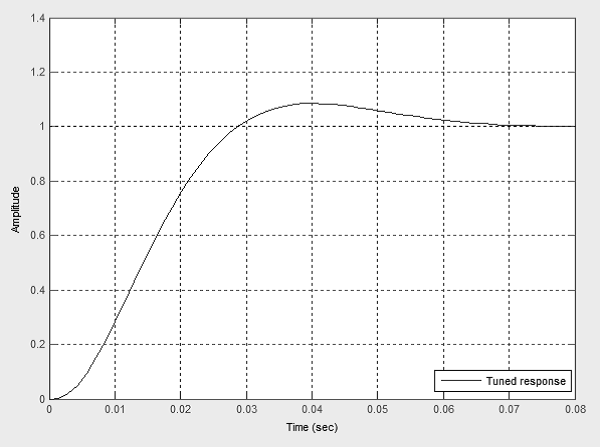
\includegraphics[width=7cm]{image11}
%\end{center} 
%
%\fi
% 
%
%\subparagraph{}
%\textit{Tracer de diagramme de Bode.}
%\ifprof
%\begin{corrige}
%\end{corrige}
%\else
%\fi
%
%\ifprof
%\else
%
%On considère $C_R (p)=0$. On prendra $K_M=\SI{0,8}{rad.s^{-1}.V^{-1}}$, $T_e=\SI{0,0051}{s}$,$T_m=\SI{0,0074}{s}$.
%\fi
%
%\subparagraph{}
%\textit{Tracer le diagramme de Bode de la fonction de transfert en boucle ouverte pour $C(p)=1$. Déterminer les marges de phase et les marges de gain.}
%\ifprof
%\begin{corrige}
%\end{corrige}
%\else
%\fi
% 
%\subparagraph{}
%\textit{Tracer le diagramme de Bode de la fonction de transfert en boucle ouverte pour $C(p)=\dfrac{1}{p}$. Déterminer les marges de phase et les marges de gain.}
%\ifprof
%\begin{corrige}
%\end{corrige}
%\else
%\fi
%
%\ifprof
%\else
%
%On donne ci-dessous les diagrammes de Bode avec les correcteurs optimisés. Déterminer les marges de gain et marges de phase. 
%\fi
%
%\section*{Vérification des performances de l'axe du magasin de rivets}
%\ifprof
%\else
%
%Afin de vérifier les réglages précédents, un essai sur le système réel est réalisé. Une consigne de \SI{2}{m} est donnée. L'absence de système d'acquisition dédié impose un système de mesure extérieur au système réel. C'est un dispositif d'analyse d'image qui est retenu pour ces mesures.
%\fi
%
%\subparagraph{}
%\textit{À partir des relevés ci-dessous, conclure sur le respect des exigences fonctionnelles de l'axe du magasin de stockage des rivets (Exigence 1.1).}
%\ifprof
%\begin{corrige}
%\end{corrige}
%\else
%\fi
 
\end{multicols}
%
%\ifprof
%\else
%
%\begin{center}
%\begin{tabular}{cc}
%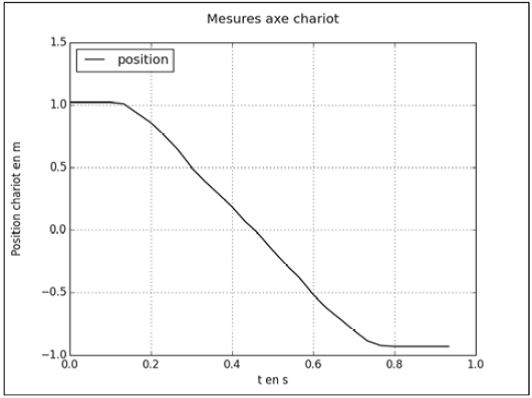
\includegraphics[width=7cm]{image13} &
%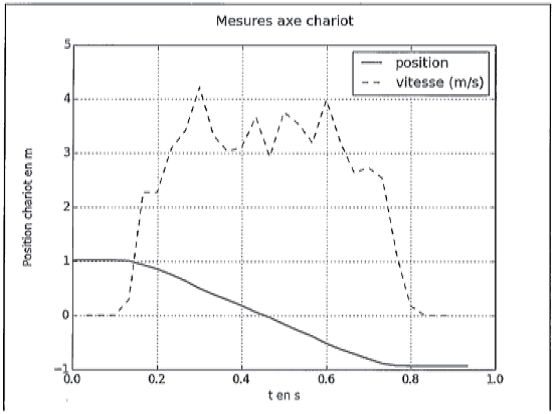
\includegraphics[width=7cm]{image14}
%
%\end{tabular}
%\end{center}
%
% \begin{center}
%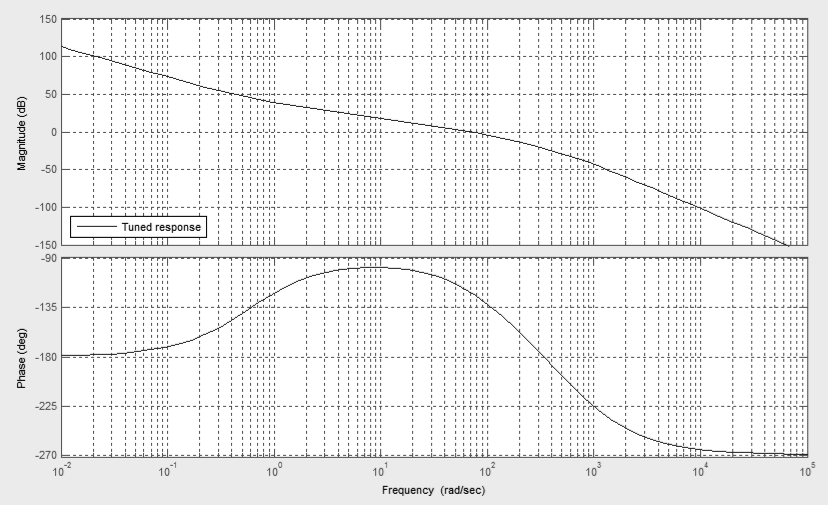
\includegraphics[width=\textwidth]{image12}
%\end{center} 
%\fi

%\end{document}


%%% PAS DE CORRIGE !!!
\newpage
\fichetrue \proftrue \tdtrue \coursfalse
\graphicspath{{../../style/png/}{../../Chapitre_03_Precision/Activation_AssemblageFalcon/images/}}
%%%%% Paramétrage du TD %%%%
\def\xxactivite{Activation\ifprof \\ \normalsize \vspace{-.4cm}Corrigé \else \fi}
\def\xxauteur{\textsl{Xavier Pessoles}}


\def\xxnumchapitre{Chapitre 3 \vspace{.2cm}}
\def\xxchapitre{\hspace{.12cm} Précision des systèmes}

\def\xxcompetences{%
\textsl{%
\textbf{Savoirs et compétences :}\\
\vspace{-.4cm}
%\begin{itemize}[label=\ding{112},font=\color{ocre}] 
%%\item \textit{Mod3.C2 : } pôles dominants et réduction de l’ordre du modèle : principe, justification
%%\item \textit{Res2.C4 : } stabilité des SLCI : définition entrée bornée -- sortie bornée (EB -- SB)	
%%\item \textit{Res2.C5 : } stabilité des SLCI : équation caractéristique	
%\item \textit{Res2.C6 : } stabilité des SLCI : position des pôles dans le plan complexe
%\item \textit{Res2.C7 : } stabilité des SLCI : marges de stabilité (de gain et de phase)
%\end{itemize}
}}


\def\xxfigures{
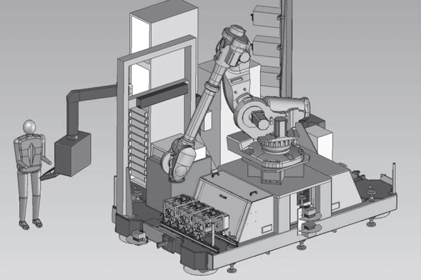
\includegraphics[width=.7\textwidth]{image1}
}%figues de la page de garde

\def\xxtitreexo{Cellule d'assemblage pour avion Falcon}
\def\xxsourceexo{D'après concours E3A -- PSI 2015.}



\iflivret
\pagestyle{empty}


%%%%%%%% PAGE DE GARDE COURS
\ifcours
\begin{tikzpicture}[remember picture,overlay]
\node at (current page.north west)
{\begin{tikzpicture}[remember picture,overlay]
\node[anchor=north west,inner sep=0pt] at (0,0) {\includegraphics[width=\paperwidth]{\thechapterimage}};
\draw[anchor=west] (-2cm,-8cm) node [line width=2pt,rounded corners=15pt,draw=ocre,fill=white,fill opacity=0.6,inner sep=40pt]{\strut\makebox[22cm]{}};
\draw[anchor=west] (1cm,-8cm) node {\huge\sffamily\bfseries\color{black} %
\begin{minipage}{1cm}
\rotatebox{90}{\LARGE\sffamily\textsc{\color{ocre}\textbf{\xxnumpartie}}}
\end{minipage} \hfill
\begin{minipage}[c]{14cm}
\begin{titrepartie}
\begin{flushright}
\renewcommand{\baselinestretch}{1.1} 
\Large\sffamily\textsc{\textbf{\xxpartie}}
\renewcommand{\baselinestretch}{1} 
\end{flushright}
\end{titrepartie}
\end{minipage} \hfill
\begin{minipage}[c]{3.5cm}
{\large\sffamily\textsc{\textbf{\color{ocre} \discipline}}}
\end{minipage} 
 };
\end{tikzpicture}};
\end{tikzpicture}


\begin{tikzpicture}[overlay]
\node[shape=rectangle, 
      rounded corners = .25 cm,
	  draw= ocre,
	  line width=2pt, 
	  fill = ocre!10,
	  minimum width  = 2.5cm,
	  minimum height = 3cm,] at (18cm,0) {};
\node at (17.7cm,0) {\rotatebox{90}{\textbf{\Large\color{ocre}{\classe}}}};
%{};
\end{tikzpicture}

\vspace{3.5cm}

\begin{tikzpicture}[remember picture,overlay]
\draw[anchor=west] (-2cm,-6cm) node {\huge\sffamily\bfseries\color{black} %
\begin{minipage}{2cm}
\begin{center}
\LARGE\sffamily\textsc{\color{ocre}\textbf{\xxactivite}}
\end{center}
\end{minipage} \hfill
\begin{minipage}[c]{15cm}
\begin{titrechapitre}
\renewcommand{\baselinestretch}{1.1} 
\Large\sffamily\textsc{\textbf{\xxnumchapitre}}

\Large\sffamily\textsc{\textbf{\xxchapitre}}
\vspace{.5cm}

\renewcommand{\baselinestretch}{1} 
\normalsize\normalfont
\xxcompetences
\end{titrechapitre}
\end{minipage}  };
\end{tikzpicture}
\vfill

\begin{flushright}
\begin{minipage}[c]{.3\linewidth}
\begin{center}
\xxfigures
\end{center}
\end{minipage}\hfill
\begin{minipage}[c]{.6\linewidth}
\startcontents
\printcontents{}{1}{}
\end{minipage}
\end{flushright}

\begin{tikzpicture}[remember picture,overlay]
\draw[anchor=west] (4.5cm,-.7cm) node {
\begin{minipage}[c]{.2\linewidth}
\begin{flushright}

\includegraphics[width=2cm]{logoCC}
\end{flushright}
\end{minipage}
\begin{minipage}[c]{.2\linewidth}
\textsl{\xxauteur} \\
\textsl{\classe}
\end{minipage}
 };
\end{tikzpicture}
\newpage
\pagestyle{fancy}

\newpage
\pagestyle{fancy}

\else
\fi


%%%%%%%% PAGE DE GARDE TD
\iftd
%\begin{tikzpicture}[remember picture,overlay]
%\node at (current page.north west)
%{\begin{tikzpicture}[remember picture,overlay]
%\draw[anchor=west] (-2cm,-3.25cm) node [line width=2pt,rounded corners=15pt,draw=ocre,fill=white,fill opacity=0.6,inner sep=40pt]{\strut\makebox[22cm]{}};
%\draw[anchor=west] (1cm,-3.25cm) node {\huge\sffamily\bfseries\color{black} %
%\begin{minipage}{1cm}
%\rotatebox{90}{\LARGE\sffamily\textsc{\color{ocre}\textbf{\xxnumpartie}}}
%\end{minipage} \hfill
%\begin{minipage}[c]{13.5cm}
%\begin{titrepartie}
%\begin{flushright}
%\renewcommand{\baselinestretch}{1.1} 
%\Large\sffamily\textsc{\textbf{\xxpartie}}
%\renewcommand{\baselinestretch}{1} 
%\end{flushright}
%\end{titrepartie}
%\end{minipage} \hfill
%\begin{minipage}[c]{3.5cm}
%{\large\sffamily\textsc{\textbf{\color{ocre} \discipline}}}
%\end{minipage} 
% };
%\end{tikzpicture}};
%\end{tikzpicture}

%%%%%%%%%% PAGE DE GARDE TD %%%%%%%%%%%%%%%
%\begin{tikzpicture}[overlay]
%\node[shape=rectangle, 
%      rounded corners = .25 cm,
%	  draw= ocre,
%	  line width=2pt, 
%	  fill = ocre!10,
%	  minimum width  = 2.5cm,
%	  minimum height = 2.5cm,] at (18.5cm,0) {};
%\node at (17.7cm,0) {\rotatebox{90}{\textbf{\Large\color{ocre}{\classe}}}};
%%{};
%\end{tikzpicture}

% PARTIE ET CHAPITRE
%\begin{tikzpicture}[remember picture,overlay]
%\draw[anchor=west] (-1cm,-2.1cm) node {\large\sffamily\bfseries\color{black} %
%\begin{minipage}[c]{15cm}
%\begin{flushleft}
%\xxnumchapitre \\
%\xxchapitre
%\end{flushleft}
%\end{minipage}  };
%\end{tikzpicture}

% Bandeau titre exo
\begin{tikzpicture}[remember picture,overlay]
\draw[anchor=west] (-2cm,-4cm) node {\huge\sffamily\bfseries\color{black} %
\begin{minipage}{5cm}
\begin{center}
\LARGE\sffamily\color{ocre}\textbf{\textsc{\xxactivite}}

\begin{center}
\xxfigures
\end{center}

\end{center}
\end{minipage} \hfill
\begin{minipage}[c]{12cm}
\begin{titrechapitre}
\renewcommand{\baselinestretch}{1.1} 
\large\sffamily\textbf{\textsc{\xxtitreexo}}

\small\sffamily{\textbf{\textit{\color{black!70}\xxsourceexo}}}
\vspace{.5cm}

\renewcommand{\baselinestretch}{1} 
\normalsize\normalfont
\xxcompetences
\end{titrechapitre}
\end{minipage}  };
\end{tikzpicture}

\else
\fi


%%%%%%%% PAGE DE GARDE FICHE
\iffiche
\begin{tikzpicture}[remember picture,overlay]
\node at (current page.north west)
{\begin{tikzpicture}[remember picture,overlay]
\draw[anchor=west] (-2cm,-3.25cm) node [line width=2pt,rounded corners=15pt,draw=ocre,fill=white,fill opacity=0.6,inner sep=40pt]{\strut\makebox[22cm]{}};
\draw[anchor=west] (1cm,-3.25cm) node {\huge\sffamily\bfseries\color{black} %
\begin{minipage}{1cm}
\rotatebox{90}{\LARGE\sffamily\textsc{\color{ocre}\textbf{\xxnumpartie}}}
\end{minipage} \hfill
\begin{minipage}[c]{14cm}
\begin{titrepartie}
\begin{flushright}
\renewcommand{\baselinestretch}{1.1} 
\large\sffamily\textsc{\textbf{\xxpartie} \\} 

\vspace{.2cm}

\normalsize\sffamily\textsc{\textbf{\xxnumchapitre -- \xxchapitre}}
\renewcommand{\baselinestretch}{1} 
\end{flushright}
\end{titrepartie}
\end{minipage} \hfill
\begin{minipage}[c]{3.5cm}
{\large\sffamily\textsc{\textbf{\color{ocre} \discipline}}}
\end{minipage} 
 };
\end{tikzpicture}};
\end{tikzpicture}


\begin{tikzpicture}[overlay]
\node[shape=rectangle, 
      rounded corners = .25 cm,
	  draw= ocre,
	  line width=2pt, 
	  fill = ocre!10,
	  minimum width  = 2.5cm,
	  minimum height = 2.5cm,] at (18.5cm,0.5cm) {};
%	  minimum height = 2.5cm,] at (18.5cm,0cm) {};
\node at (17.7cm,0.5) {\rotatebox{90}{\textsf{\textbf{\large\color{ocre}{\classe}}}}};
%{};
\end{tikzpicture}



\else
\fi



\else
\pagestyle{empty}


%%%%%%%% PAGE DE GARDE COURS
\ifcours
\begin{tikzpicture}[remember picture,overlay]
\node at (current page.north west)
{\begin{tikzpicture}[remember picture,overlay]
\node[anchor=north west,inner sep=0pt] at (0,0) {\includegraphics[width=\paperwidth]{\thechapterimage}};
\draw[anchor=west] (-2cm,-8cm) node [line width=2pt,rounded corners=15pt,draw=ocre,fill=white,fill opacity=0.6,inner sep=40pt]{\strut\makebox[22cm]{}};
\draw[anchor=west] (1cm,-8cm) node {\huge\sffamily\bfseries\color{black} %
\begin{minipage}{1cm}
\rotatebox{90}{\LARGE\sffamily\textsc{\color{ocre}\textbf{\xxnumpartie}}}
\end{minipage} \hfill
\begin{minipage}[c]{14cm}
\begin{titrepartie}
\begin{flushright}
\renewcommand{\baselinestretch}{1.1} 
\Large\sffamily\textsc{\textbf{\xxpartie}}
\renewcommand{\baselinestretch}{1} 
\end{flushright}
\end{titrepartie}
\end{minipage} \hfill
\begin{minipage}[c]{3.5cm}
{\large\sffamily\textsc{\textbf{\color{ocre} \discipline}}}
\end{minipage} 
 };
\end{tikzpicture}};
\end{tikzpicture}


\begin{tikzpicture}[overlay]
\node[shape=rectangle, 
      rounded corners = .25 cm,
	  draw= ocre,
	  line width=2pt, 
	  fill = ocre!10,
	  minimum width  = 2.5cm,
	  minimum height = 3cm,] at (18cm,0) {};
\node at (17.7cm,0) {\rotatebox{90}{\textbf{\Large\color{ocre}{\classe}}}};
%{};
\end{tikzpicture}

\vspace{3.5cm}

\begin{tikzpicture}[remember picture,overlay]
\draw[anchor=west] (-2cm,-6cm) node {\huge\sffamily\bfseries\color{black} %
\begin{minipage}{2cm}
\begin{center}
\LARGE\sffamily\textsc{\color{ocre}\textbf{\xxactivite}}
\end{center}
\end{minipage} \hfill
\begin{minipage}[c]{15cm}
\begin{titrechapitre}
\renewcommand{\baselinestretch}{1.1} 
\Large\sffamily\textsc{\textbf{\xxnumchapitre}}

\Large\sffamily\textsc{\textbf{\xxchapitre}}
\vspace{.5cm}

\renewcommand{\baselinestretch}{1} 
\normalsize\normalfont
\xxcompetences
\end{titrechapitre}
\end{minipage}  };
\end{tikzpicture}
\vfill

\begin{flushright}
\begin{minipage}[c]{.3\linewidth}
\begin{center}
\xxfigures
\end{center}
\end{minipage}\hfill
\begin{minipage}[c]{.6\linewidth}
\startcontents
\printcontents{}{1}{}
\end{minipage}
\end{flushright}

\begin{tikzpicture}[remember picture,overlay]
\draw[anchor=west] (4.5cm,-.7cm) node {
\begin{minipage}[c]{.2\linewidth}
\begin{flushright}

\includegraphics[width=2cm]{logoCC}
\end{flushright}
\end{minipage}
\begin{minipage}[c]{.2\linewidth}
\textsl{\xxauteur} \\
\textsl{\classe}
\end{minipage}
 };
\end{tikzpicture}
\newpage
\pagestyle{fancy}

\newpage
\pagestyle{fancy}

\else
\fi


%%%%%%%% PAGE DE GARDE TD
\iftd
%\begin{tikzpicture}[remember picture,overlay]
%\node at (current page.north west)
%{\begin{tikzpicture}[remember picture,overlay]
%\draw[anchor=west] (-2cm,-3.25cm) node [line width=2pt,rounded corners=15pt,draw=ocre,fill=white,fill opacity=0.6,inner sep=40pt]{\strut\makebox[22cm]{}};
%\draw[anchor=west] (1cm,-3.25cm) node {\huge\sffamily\bfseries\color{black} %
%\begin{minipage}{1cm}
%\rotatebox{90}{\LARGE\sffamily\textsc{\color{ocre}\textbf{\xxnumpartie}}}
%\end{minipage} \hfill
%\begin{minipage}[c]{13.5cm}
%\begin{titrepartie}
%\begin{flushright}
%\renewcommand{\baselinestretch}{1.1} 
%\Large\sffamily\textsc{\textbf{\xxpartie}}
%\renewcommand{\baselinestretch}{1} 
%\end{flushright}
%\end{titrepartie}
%\end{minipage} \hfill
%\begin{minipage}[c]{3.5cm}
%{\large\sffamily\textsc{\textbf{\color{ocre} \discipline}}}
%\end{minipage} 
% };
%\end{tikzpicture}};
%\end{tikzpicture}

%%%%%%%%%% PAGE DE GARDE TD %%%%%%%%%%%%%%%
%\begin{tikzpicture}[overlay]
%\node[shape=rectangle, 
%      rounded corners = .25 cm,
%	  draw= ocre,
%	  line width=2pt, 
%	  fill = ocre!10,
%	  minimum width  = 2.5cm,
%	  minimum height = 2.5cm,] at (18.5cm,0) {};
%\node at (17.7cm,0) {\rotatebox{90}{\textbf{\Large\color{ocre}{\classe}}}};
%%{};
%\end{tikzpicture}

% PARTIE ET CHAPITRE
%\begin{tikzpicture}[remember picture,overlay]
%\draw[anchor=west] (-1cm,-2.1cm) node {\large\sffamily\bfseries\color{black} %
%\begin{minipage}[c]{15cm}
%\begin{flushleft}
%\xxnumchapitre \\
%\xxchapitre
%\end{flushleft}
%\end{minipage}  };
%\end{tikzpicture}

% Bandeau titre exo
\begin{tikzpicture}[remember picture,overlay]
\draw[anchor=west] (-2cm,-4cm) node {\huge\sffamily\bfseries\color{black} %
\begin{minipage}{5cm}
\begin{center}
\LARGE\sffamily\color{ocre}\textbf{\textsc{\xxactivite}}

\begin{center}
\xxfigures
\end{center}

\end{center}
\end{minipage} \hfill
\begin{minipage}[c]{12cm}
\begin{titrechapitre}
\renewcommand{\baselinestretch}{1.1} 
\large\sffamily\textbf{\textsc{\xxtitreexo}}

\small\sffamily{\textbf{\textit{\color{black!70}\xxsourceexo}}}
\vspace{.5cm}

\renewcommand{\baselinestretch}{1} 
\normalsize\normalfont
\xxcompetences
\end{titrechapitre}
\end{minipage}  };
\end{tikzpicture}

\else
\fi


%%%%%%%% PAGE DE GARDE FICHE
\iffiche
\begin{tikzpicture}[remember picture,overlay]
\node at (current page.north west)
{\begin{tikzpicture}[remember picture,overlay]
\draw[anchor=west] (-2cm,-3.25cm) node [line width=2pt,rounded corners=15pt,draw=ocre,fill=white,fill opacity=0.6,inner sep=40pt]{\strut\makebox[22cm]{}};
\draw[anchor=west] (1cm,-3.25cm) node {\huge\sffamily\bfseries\color{black} %
\begin{minipage}{1cm}
\rotatebox{90}{\LARGE\sffamily\textsc{\color{ocre}\textbf{\xxnumpartie}}}
\end{minipage} \hfill
\begin{minipage}[c]{14cm}
\begin{titrepartie}
\begin{flushright}
\renewcommand{\baselinestretch}{1.1} 
\large\sffamily\textsc{\textbf{\xxpartie} \\} 

\vspace{.2cm}

\normalsize\sffamily\textsc{\textbf{\xxnumchapitre -- \xxchapitre}}
\renewcommand{\baselinestretch}{1} 
\end{flushright}
\end{titrepartie}
\end{minipage} \hfill
\begin{minipage}[c]{3.5cm}
{\large\sffamily\textsc{\textbf{\color{ocre} \discipline}}}
\end{minipage} 
 };
\end{tikzpicture}};
\end{tikzpicture}


\begin{tikzpicture}[overlay]
\node[shape=rectangle, 
      rounded corners = .25 cm,
	  draw= ocre,
	  line width=2pt, 
	  fill = ocre!10,
	  minimum width  = 2.5cm,
	  minimum height = 2.5cm,] at (18.5cm,0.5cm) {};
%	  minimum height = 2.5cm,] at (18.5cm,0cm) {};
\node at (17.7cm,0.5) {\rotatebox{90}{\textsf{\textbf{\large\color{ocre}{\classe}}}}};
%{};
\end{tikzpicture}



\else
\fi



\fi
\setlength{\columnseprule}{.1pt}

\pagestyle{fancy}
\thispagestyle{plain}


\vspace{4.5cm}

\def\columnseprulecolor{\color{ocre}}
\setlength{\columnseprule}{0.4pt} 

%%%%%%%%%%%%%%%%%%%%%%%


\begin{multicols}{2}
\setcounter{exo}{0}
\subsection*{Présentation}
Le tronçon central du fuselage du Falcon 7X est assemblé par rivetage grâce à un robot 6 axes. Les rivets sont stockés dans des cassettes rangées verticalement. Un chariot de sélection se déplace verticalement pour déplacer une buse d'aspiration qui permettra d'acheminer les rivets contenus dans la cassette vers l'effecteur (robot). Le chariot fait l'objet de cette étude.

\begin{center}
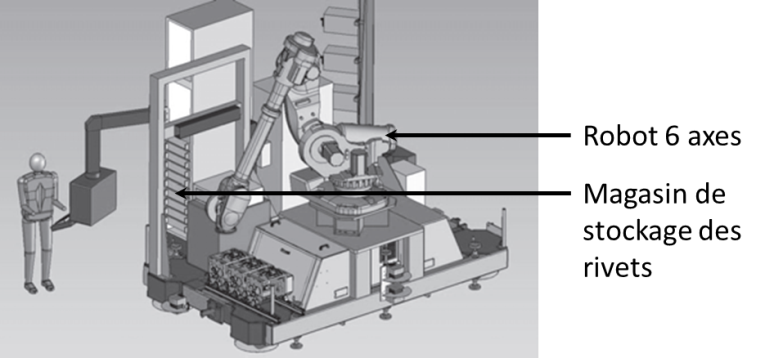
\includegraphics[width=7cm]{image5}
\end{center} 

\begin{obj}
Vérifier que les correcteurs proposés permettent ou non d'obtenir un écart statique nul et un écart en vitesse nul.
\end{obj}
% 
%L'objectif de cette partie est de valider les choix effectués par la société pour le sous ensemble de sélection des fixations de la cellule (exigence 1.1).

%\vfill
%
%\begin{center}
%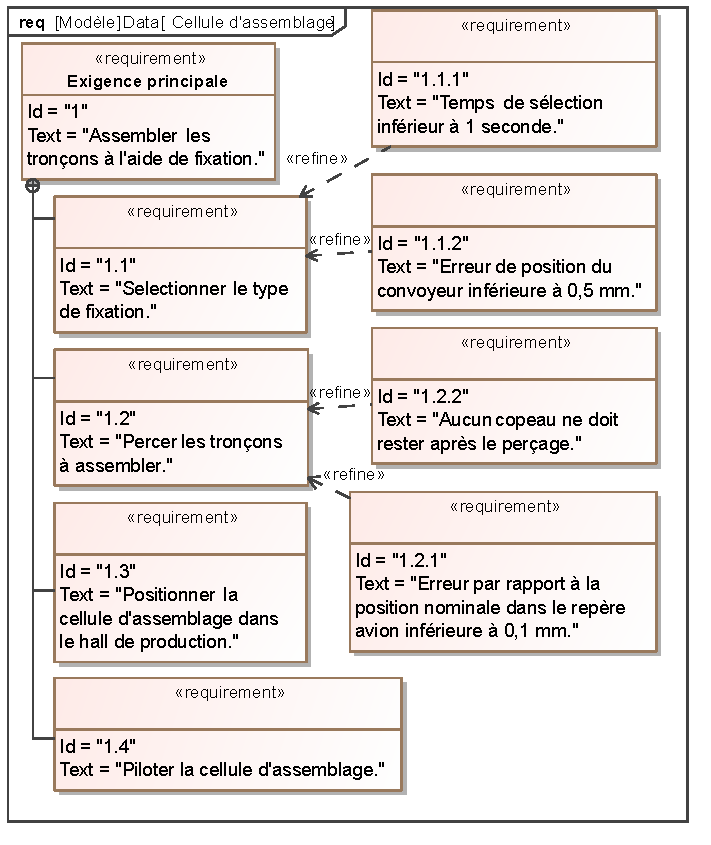
\includegraphics[width=7cm]{Exigences}
%\end{center} 




% 
%\subsection*{Axe chariot}
%Le déplacement du chariot est assuré par un axe numérique asservi en vitesse et en position. Cet axe est composé d'un moteur à courant continu, d'un système de transmission de puissance de type poulies / courroie et d'un rail.
% 
%\begin{center}
%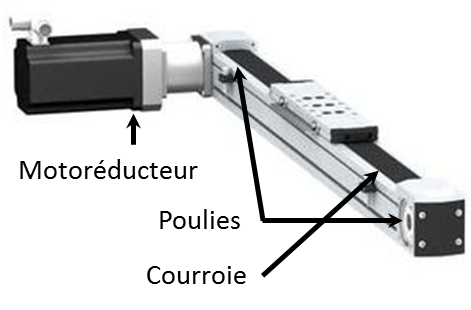
\includegraphics[width=4.5cm]{image7}
%\end{center} 
%
%
%\subsection*{Modélisation du système de déplacement du chariot}
%
%\begin{center}
%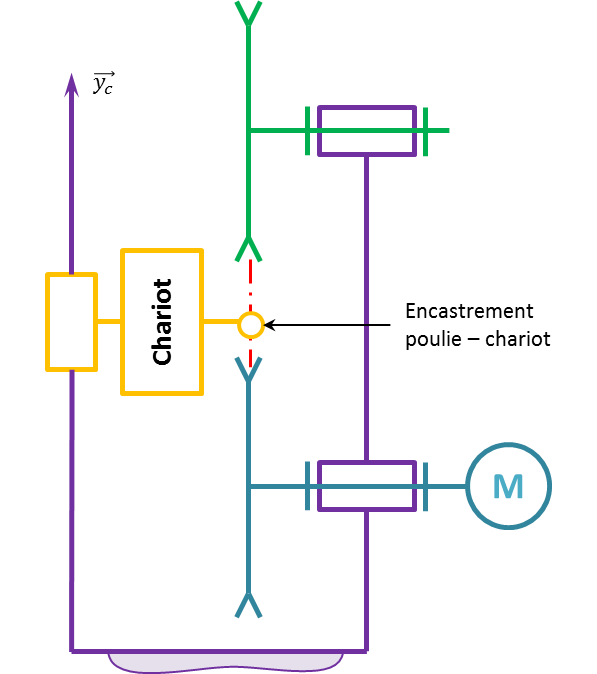
\includegraphics[width=5cm]{image8}
%\end{center} 
%
%
%\fi

%
%
%
%\section*{Sélectionner les fixations – Exigence 1.1}
%\ifprof
%\else 
%Afin de sélectionner le type de fixation, la buse d'aspiration doit être déplacée en face de la cassette avec une erreur inférieure à $\SI{0,5}{mm}$ (voir exigences fonctionnelles). Cependant le fabricant du système poulie-courroie du rail indique déjà une erreur de $\pm \SI{0,25}{mm}$ due notamment à l'élasticité de la courroie. Par conséquent, l'erreur en position de la commande doit être nulle. De plus, afin de ne pas perdre de temps lors de la production, le temps maximal de déplacement lors de la sélection est imposé à une seconde.
%
%L'étude se fera dans le cas le plus défavorable c'est-à-dire un déplacement du chariot vers le haut entre les deux cassettes de rivets les plus éloignées. L'axe de déplacement est appelé $\vect{y_c}$
%\subsection*{Notations domaine temporel – domaine de Laplace}
%
%Les notations entre le domaine temporel et celui de Laplace sont données dans la suite. Ainsi, si la fonction $f(t)$ possède une transformée de Laplace, elle sera notée : $F(p) = \mathcal{L}[f(t)]$.
%Les équations caractéristiques du moteur à courant continu sont rappelées ci-dessous (les conditions de Heaviside sont respectées) :
%\begin{itemize}[label=\ding{112},font=\color{ocre}] 
%\item $u(t)=e(t)+L \dfrac{di(t)}{\text{d} t}+Ri(t)$;
%\item $e(t)=K_E \omega_m (t)$ ;
%\item $C_M (t)=K_C i(t)$ ;
%\item $J_{eq}  \dfrac{d\omega_m)}{\text{d} t}+f\omega_m (t)=C_M (t)-C_R (t)$.
%\end{itemize}
%
%Avec : 
%\begin{itemize}[label=\ding{112},font=\color{ocre}] 
%\item $u(t)$ : tension moteur ;
%\item $i(t)$ : courant moteur ; 
%\item $e(t)$ : force contre-électromotrice ;
%\item $\omega_m(t)$ : vitesse de rotation moteur ;
%\item $C_M (t)$ : couple moteur ;
%\item $C_R (t)$: couple résistant modélisant l'action de pesanteur.
%\end{itemize}
%\fi
%
%\subsection*{Critères à respecter pour l'exigence 1.2}
%\ifprof
%\else
%\footnotesize{
%\begin{center}
%\begin{tabular}{|p{2cm}|p{2.5cm}|p{2cm}|}
%\hline
%Exigence	& Critères & Niveaux \\ \hline
%Déplacer le chariot	& Précision :
%erreur statique par rapport à une consigne de vitesse constante	
%& NULLE \\ \hline
%	& Rapidité : temps de réponse à 5\% en réponse à une consigne échelon 
%	& $Tr_{5\%} = \SI{0,1}{s}$  maxi \\ \hline
%	& Stabilité : & \\
%	& Marge de gain & \SI{6}{dB} mini \\
%	&Marge de gain & $\ang{45}$ mini \\
%\hline
%\end{tabular}
%\end{center}}

%\fi
%\subsection*{Choix d'une architecture de la chaine de transmission}
%\subparagraph{}
%\textit{Proposer sous la forme d'un schéma une autre solution permettant le déplacement du chariot. La conversion de l'énergie électrique en énergie mécanique par un moteur doit être conservée.}
%
%\ifprof
%\begin{corrige}
%Utilisation d’un système vis-écrou.
%\end{corrige}
%\else
%\fi
%
%\ifprof
%\else
%Compte tenu des vitesses de translation importantes, le système retenu est de type poulie-courroie.
%\fi
%
%\subsection*{Détermination de l'inertie équivalente} 
%\ifprof
%\else
%
%Les grandeurs caractéristiques (notations et valeurs) des éléments de l'axe du chariot sont données dans le tableau ci-dessous :
%\begin{center}
%\begin{tabular}{|p{3cm}|c|c|}
%\hline
%Moment d'inertie du rotor du moteur autour de son axe&	$J_m$ & $\num{140d-6}\si{kg.m^2}$ \\ \hline
%Moment d'inertie du réducteur ramené à l'arbre moteur&	$J_{réd}$ & $\num{60d-4}\si{kg.m^2}$ \\ \hline
%Moment d'inertie de la poulie motrice autour de son axe&	$J_{PM}$	&$ \num{38d-4}\si{kg.m^2}$ \\ \hline
%Moment d'inertie de la poulie réceptrice autour de son axe&	$J_{PR}$ & $\num{38d-4}\si{kg.m^2}$ \\ \hline
%Masse totale du chariot	&$M$ &$\SI{5}{kg}$ \\ \hline
%Vitesse de rotation de l'arbre moteur &$\omega_m$ &  \\ \hline
%Vitesse de rotation de l'arbre de sortie du réducteur	&$\omega_r$&  \\ \hline
%Rayon d'une poulie motrice ou réceptrice	& $R_P$ &$\SI{45}{mm}$ \\ \hline
%Rapport de réduction réducteur ($\omega_r/\omega_m$)	& $\lambda$	&$1/5$ \\ \hline
%\end{tabular}
%\end{center}
%\fi
%
%\subparagraph{}
%\textit{À partir des grandeurs définies déterminer l'expression littérale de l'inertie équivalente $J_{eq}$ de l'ensemble $\Sigma=$\{moteur+réducteur+poulies+chariot\} ramenée sur l'arbre moteur. Cette inertie équivalente est définie par $E_c (\Sigma)=1/2 J_{eq} \omega_m^2$.}
%\ifprof
%\begin{corrige}
%$\mathcal{E}_c(\Sigma)=\mathcal{E}_c (\text{moteur})+\mathcal{E}_c (\text{réducteur})+\mathcal{E}_c (\text{poulies})+\mathcal{E}_c (\text{chariot})$.
%\begin{itemize}
%	\item $\mathcal{E}_c (\text{moteur})=1/2 J_m \omega_m^2$;
%	\item $\mathcal{E}_c (\text{réducteur})=1/2 J_{\text{red}} \omega_m^2$;
%	\item $\mathcal{E}_c (\text{poulies})=1/2 (J_{\text{Pm}}+J_{\text{PR}}  ) \omega_{\text{red}}^2=1/2 (J_{\text{Pm}}+J_{\text{PR}}  ) \lambda^2 \omega_m^2$;
%	\item $\mathcal{E}_c (\text{chariot})=1/2 MV^2=1/2 MR_p^2 \lambda^2 \omega_m^2$.
%\end{itemize}
%On a donc $J_{\text{eq}}=MR_p^2 \lambda^2+(J_{\text{Pm}}+J_{\text{PR}}  ) \lambda^2+J_{\text{red}}+J_m$.
%
%\end{corrige}
%\else
%\fi
%
%\subparagraph{}
%\textit{Déterminer la valeur numérique de l'expression précédente.}
%\ifprof
%\begin{corrige}
%$J_{eq}=\SI{0,0068}{kg.m^2}$
%\end{corrige}
%\else
%\fi
%
%\subsection*{Modèle de connaissance du moteur à courant continu}
%
%\begin{obj}
%L'objectif de cette partie est d'établir un modèle de la motorisation de l'axe afin de simuler un déplacement.
%\end{obj}
%
%\subparagraph{}
%\textit{À partir des équations du moteur à courant continu, réaliser le schéma bloc du moteur à courant continu.}
%\ifprof
%\begin{corrige} ~\\
%
%\begin{center}
%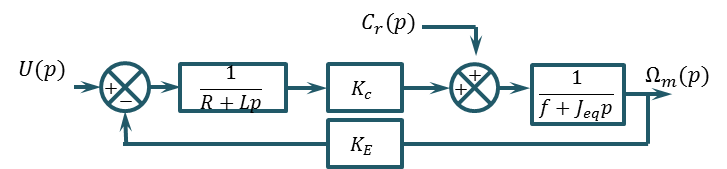
\includegraphics[width=7cm]{corr_01}
%\end{center} 
%\end{corrige}
%\else
%\fi
%
%\subparagraph{}
%\textit{En considérant que $C_R (p)=0$, déterminer la fonction de transfert $H_M (p)=\dfrac{\Omega_m (p)}{U(p)}$ sous sa forme canonique.}
%\ifprof
%\begin{corrige}
%$H_m (p)=\dfrac{\dfrac{K_C}{K_c K_E+Rf}}{1+\dfrac{RJ_eq+Lf}{K_c K_E+Rf}p+\dfrac{LJ_eq}{K_c K_E+Rf} p^2}$
%\end{corrige}
%\else
%\fi
%
%\subparagraph{}
%\textit{Montrer que la fonction de transfert $H_M (p)$ peut se mettre sous la forme $H_M (p)=\dfrac{K_C}{K_C K_e+RJ_{eq} p+LJ_{eq} p^2 }$. Justifier la réponse. Pour cette question, la valeur numérique de $J_{eq}$ considérée sera $J_{eq}=\num{7d-3}\si{kg.m^2}$ indépendamment du résultat numérique calculé précédemment.}
%\ifprof
%\begin{corrige}
%En faisant les applications numériques on montre que $Rf$ est négligeable devant $K_c K_E$ et que $Lf$ et négligeable devant $RJ_{eq}$. On a donc : 
%$H_m (p)=\dfrac{\dfrac{K_C}{K_c K_E}}{1+\dfrac{RJ_{eq}}{K_c K_E }p+\dfrac{LJ_{eq}}{K_c K_E }p^2 }=\dfrac{K_C}{K_c K_E+RJ_{eq} p+LJ_{eq} p^2 }$.
%
%\end{corrige}
%\else
%\fi
%
%\subparagraph{}
%\textit{Montrer qu'avec l'expression, $H_M (p)$ peut s'écrire sous la forme $H_M (p)=\dfrac{K_M}{(1+T_E p)(1+T_M p)}$  avec $T_E<T_M$.}
%\ifprof
%\begin{corrige}
%$
%\left\{
%\begin{array}{l}
%T_e+T_m= \dfrac{RJ_{eq}}{K_c K_e}\\
%T_e T_m=\dfrac{LJ_{eq}}{K_C K_e}
%\end{array}
%\right.
%$
%On a (résolution d’une équation du second degré):
%
%$Te=\dfrac{\dfrac{RJ_{eq}}{K_c K_e}-\sqrt{\left(\dfrac{RJ_{eq}}{K_c K_e}\right)^2 - 4\dfrac{LJ_{eq}}{K_c K_e}}}{2}$. $T_e=\SI{0,0051}{s}$ et $T_m=\SI{0,0074}{s}$.
%
%
%\end{corrige}
%\else
%\fi
%\section*{Étude de l'asservissement en position de l'axe}
%\subsection*{Modélisation de l'asservissement en position}
%\ifprof
%\else
%
%
%La partie précédente a permis de déterminer un modèle du moteur. La suite de l'étude va permettre, par simulation, de déterminer les réglages nécessaires de l'axe vis-à-vis du cahier des charges. La figure suivante présente le principe de l'asservissement de l'axe du chariot.
% 
%\begin{center}
%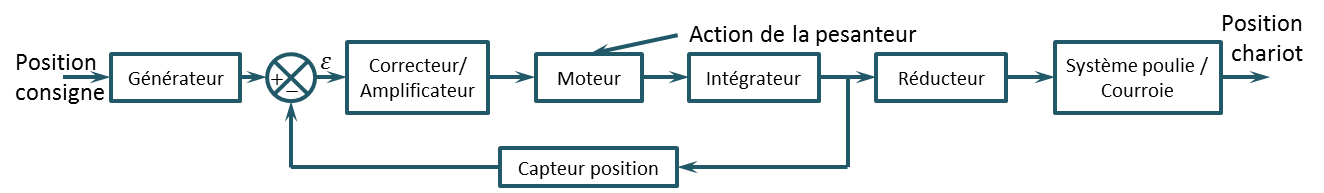
\includegraphics[width=7cm]{image9}
%\end{center} 
%
%Les grandeurs caractéristiques des blocs de l'asservissement de l'axe chariot sont données dans le tableau ci-dessous :
%\begin{center}
%\begin{tabular}{|c|c|c|}
%\hline
%Générateur & $K_G$ & À déterminer \\
%\hline
%Capteur de position	& $K_\text{capt}$ & $\num{5d-3}\si{V.rad^(-1)}$ \\
%\hline
%Correcteur amplificateur	 & $C(p)$ & Variable \\
%\hline
%\end{tabular}
%\end{center}
%\fi
%
%\subparagraph{}
%\textit{Quelle doit être la valeur de $K_G$ pour assurer un asservissement correct (c'est-à-dire l'écart $\varepsilon$ doit être nul si la position de l'axe est identique à la consigne) ?}
%\ifprof
%\begin{corrige} ~\\
%
%On doit avoir $K_G=K_{\text{capt}} \dfrac{1}{\lambda} \dfrac{1}{R_p}=\SI{0,556}{V.rad^{-1}.m^{-1}}$.
%\end{corrige}
%\else
%\fi
%
%\subparagraph{}
%\textit{Donner le schéma-blocs de l'asservissement.}
%\ifprof
%\begin{corrige} ~\\
%
%\begin{center}
%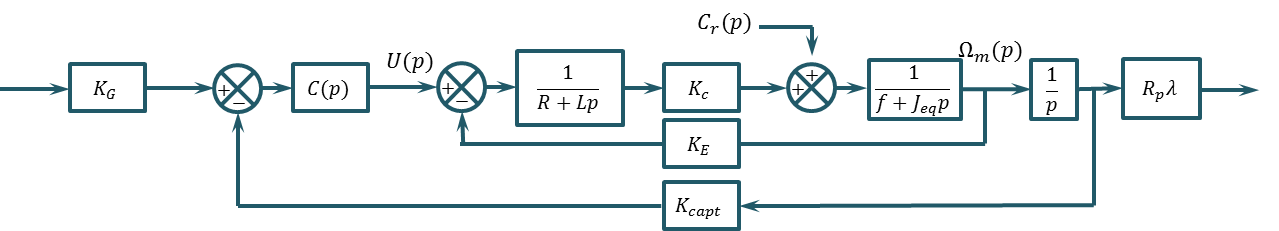
\includegraphics[width=7cm]{corr_02}
%\end{center} 
%
%\end{corrige}
%\else
%\fi

\subsection*{Étude du modèle simplifié}
\ifprof
\else
Afin de faciliter les calculs, le schéma bloc à retour unitaire est donné figure suivante. Le couple résistant $C_r$ dû à l'action de pesanteur est supposé constant.
 
 \begin{center}
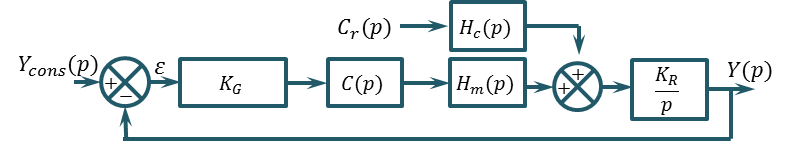
\includegraphics[width=\linewidth]{image10}
\end{center} 


Avec : 

\noindent $H_M (p)=\dfrac{K_M}{(1+T_E p)(1+T_M p)} \text{ et }
H_C (p)=\dfrac{\dfrac{\left(R+Lp\right)K_M}{K_C}}{(1+T_E p)(1+T_M p)}$.
%\item $C_R (p)=C_r/p$;
%\item $K_R=R_p \lambda$.
%\end{itemize}
\fi

\subparagraph{}
\textit{Donner l'expression de $\varepsilon(p)$.}
\ifprof
\begin{corrige}~\\
On raisonne par superposition :

Si $C_r (p)=0$: 

$$Y_1 (p)
=Y_{\text{cons}}(p) \dfrac{\dfrac{K_G K_{\text{Capt}} C(p) H_m (p) K_r}{p}}{1+\dfrac{K_G K_{\text{Capt}} C(p) H_m (p) K_r}{p}}$$

$$
=Y_{\text{cons}} (p) \dfrac{K_G K_{\text{Capt}} C(p) H_m (p) K_r}{p+K_G K_{\text{Capt}} C(p) H_m (p) K_r } 
$$

$$
=Y_{\text{cons}} (p) \dfrac{K_G K_{\text{Capt}} C(p) K_M  K_r}{(1+T_E p)(1+T_M p)p+K_G K_{\text{Capt}} C(p) K_M K_r )}$$.

\end{corrige}

\begin{corrige}
Si $Y_{\text{Cons}} (p)=0$ :

$$Y_2 (p)
=C_r (p) \dfrac{\dfrac{H_c (p) K_r}{p}}{1+\dfrac{K_r K_G K_{\text{Capt}} C(p) H_m (p)}{p} }$$

$$
=C_r (p) \dfrac{H_c (p) K_r}{p+K_r K_G K_{\text{Capt}} C(p) H_m (p) }$$
$$
=C_r (p) \dfrac{\dfrac{(R+Lp) K_M  K_r}{K_C }}{(1+T_E p)(1+T_M p)p+K_r K_G K_{\text{Capt}} C(p) K_M }$$

On a donc :
$Y(p)=Y_1 (p)+Y_2 (p)$.

\end{corrige}
\else
\fi

\subparagraph{}
\textit{On souhaite déterminer l'erreur en position du système. Calculer l'écart statique pour $C(p)=K_p$. Pouvait-on prévoir le résultat ?}
\ifprof
\begin{corrige}
\end{corrige}
\else
\fi


\subparagraph{}
\textit{On souhaite déterminer l'erreur en position du système. Calculer l'écart statique pour $C(p)=\dfrac{K_i}{p}$. Pouvait-on prévoir le résultat ?}
\ifprof
\begin{corrige}
\end{corrige}
\else
\fi


\subparagraph{}
\textit{On souhaite déterminer l'erreur en vitesse du système. Calculer l'erreur pour $C(p)=\dfrac{K_i}{p}$. Pouvait-on prévoir le résultat ?}
\ifprof
\begin{corrige}
\end{corrige}
\else
\fi


\subparagraph{}
\textit{On souhaite déterminer l'erreur pour un entrée en position du système avec une perturbation de type rampe. Calculer l'erreur pour $C(p)=\dfrac{K_i}{p}$. Pouvait-on prévoir le résultat ?}
\ifprof
\begin{corrige}
\end{corrige}
\else
\fi

%
%\subparagraph{}
%\textit{On souhaite que lorsque le système se déplace à vitesse constante, l'erreur sur la vitesse atteinte par le système soit nulle. Quelle sollicitation doit-on utiliser. Calculer l'écart statique pour $C(p)=K_p$ puis $C(p)=\dfrac{K_i}{p}$.}
%\ifprof
%\begin{corrige}
%\end{corrige}
%\else
%\fi
%
%\subparagraph{}
%\textit{Conclure.}
%\ifprof
%\begin{corrige}
%\end{corrige}
%\else
%\fi

%\ifprof
%\else
%
%Afin de répondre totalement au cahier des charges, l'utilisation d'un correcteur proportionnel intégral dérivé est retenue. En effet, la commande de l'axe intègre directement ce type de correcteur. Dans la suite du problème, le correcteur $C(p)$ sera de la forme : $C(p)=K_I \left(1+\dfrac{1}{(T_I p}\right)\left(1+T_D p\right)$. Le réglage des coefficients a été fait par simulation numérique.
%Afin de vérifier maintenant le critère de rapidité, on donne la réponse temporelle (figure page suivante) de l'axe à un échelon de position de $\SI{1}{m}$.
%
%\fi
%
%\subparagraph{}
%\textit{Conclure sur la conformité au cahier des charges du système ainsi réglé.}
%\ifprof
%\begin{corrige}
%\end{corrige}
%\else
%\fi
%
%\ifprof
%\else
% 
% \begin{center}
%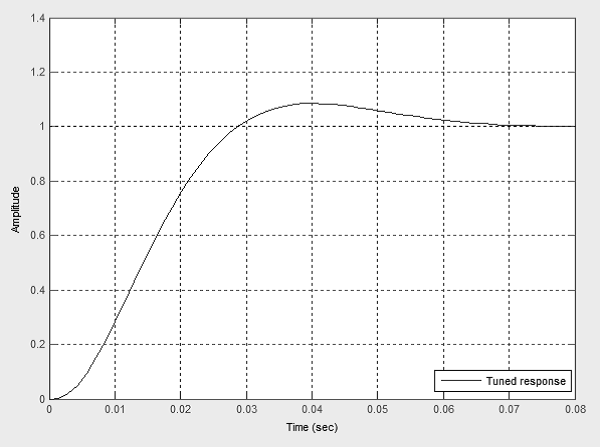
\includegraphics[width=7cm]{image11}
%\end{center} 
%
%\fi
% 
%
%\subparagraph{}
%\textit{Tracer de diagramme de Bode.}
%\ifprof
%\begin{corrige}
%\end{corrige}
%\else
%\fi
%
%\ifprof
%\else
%
%On considère $C_R (p)=0$. On prendra $K_M=\SI{0,8}{rad.s^{-1}.V^{-1}}$, $T_e=\SI{0,0051}{s}$,$T_m=\SI{0,0074}{s}$.
%\fi
%
%\subparagraph{}
%\textit{Tracer le diagramme de Bode de la fonction de transfert en boucle ouverte pour $C(p)=1$. Déterminer les marges de phase et les marges de gain.}
%\ifprof
%\begin{corrige}
%\end{corrige}
%\else
%\fi
% 
%\subparagraph{}
%\textit{Tracer le diagramme de Bode de la fonction de transfert en boucle ouverte pour $C(p)=\dfrac{1}{p}$. Déterminer les marges de phase et les marges de gain.}
%\ifprof
%\begin{corrige}
%\end{corrige}
%\else
%\fi
%
%\ifprof
%\else
%
%On donne ci-dessous les diagrammes de Bode avec les correcteurs optimisés. Déterminer les marges de gain et marges de phase. 
%\fi
%
%\section*{Vérification des performances de l'axe du magasin de rivets}
%\ifprof
%\else
%
%Afin de vérifier les réglages précédents, un essai sur le système réel est réalisé. Une consigne de \SI{2}{m} est donnée. L'absence de système d'acquisition dédié impose un système de mesure extérieur au système réel. C'est un dispositif d'analyse d'image qui est retenu pour ces mesures.
%\fi
%
%\subparagraph{}
%\textit{À partir des relevés ci-dessous, conclure sur le respect des exigences fonctionnelles de l'axe du magasin de stockage des rivets (Exigence 1.1).}
%\ifprof
%\begin{corrige}
%\end{corrige}
%\else
%\fi
 
\end{multicols}
%
%\ifprof
%\else
%
%\begin{center}
%\begin{tabular}{cc}
%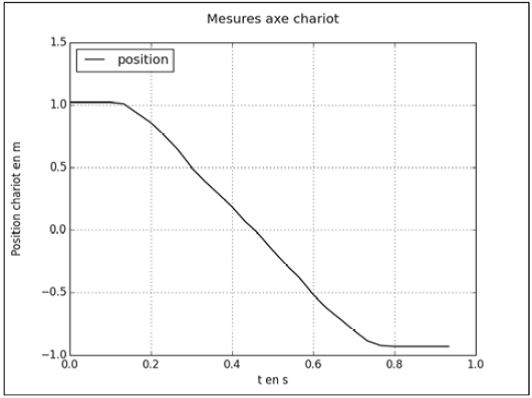
\includegraphics[width=7cm]{image13} &
%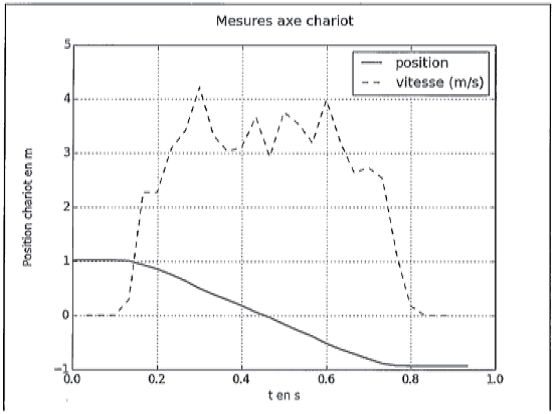
\includegraphics[width=7cm]{image14}
%
%\end{tabular}
%\end{center}
%
% \begin{center}
%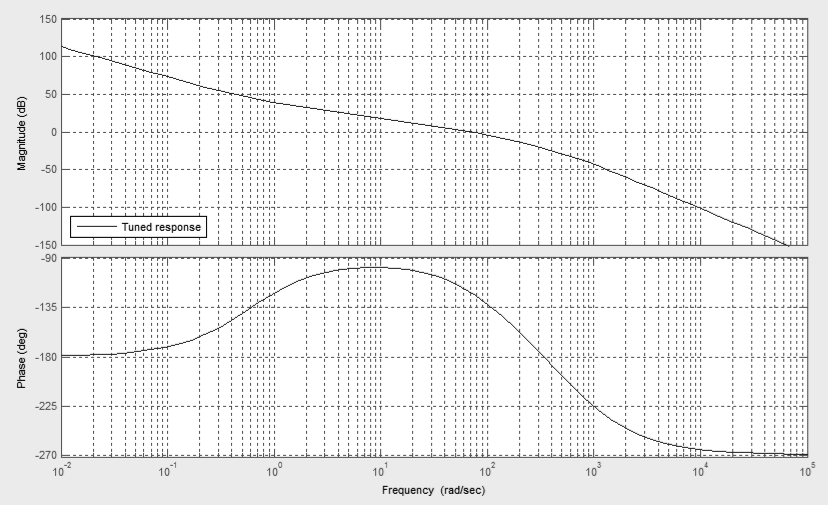
\includegraphics[width=\textwidth]{image12}
%\end{center} 
%\fi

%\end{document}


% Application
% Sujet
\newpage
\fichetrue \proffalse \tdtrue \coursfalse
\graphicspath{{../../style/png/}{../../Chapitre_03_Precision/Application_01/images/}}
%%%% Paramétrage du TD %%%%
\def\xxactivite{Application \ifprof \\ Corrigé \else \fi} % \normalsize \vspace{-.4cm}
\def\xxauteur{\textsl{Xavier Pessoles}}


\def\xxnumchapitre{Chapitre 3 \vspace{.2cm}}
\def\xxchapitre{\hspace{.12cm} Précision des systèmes}

\def\xxcompetences{%
\textsl{%
\textbf{Savoirs et compétences :}\\
\vspace{-.4cm}
%\begin{itemize}[label=\ding{112},font=\color{ocre}] 
%%\item \textit{Mod3.C2 : } pôles dominants et réduction de l’ordre du modèle : principe, justification
%%\item \textit{Res2.C4 : } stabilité des SLCI : définition entrée bornée -- sortie bornée (EB -- SB)	
%%\item \textit{Res2.C5 : } stabilité des SLCI : équation caractéristique	
%\item \textit{Res2.C6 : } stabilité des SLCI : position des pôles dans le plan complexe
%\item \textit{Res2.C7 : } stabilité des SLCI : marges de stabilité (de gain et de phase)
%\end{itemize}
}}


\def\xxfigures{
%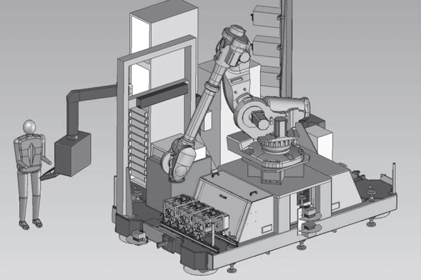
\includegraphics[width=.7\textwidth]{image1}
}%figues de la page de garde

\def\xxtitreexo{Application}
\def\xxsourceexo{}%D'après concours E3A -- PSI 2015.}



\iflivret
\pagestyle{empty}


%%%%%%%% PAGE DE GARDE COURS
\ifcours
\begin{tikzpicture}[remember picture,overlay]
\node at (current page.north west)
{\begin{tikzpicture}[remember picture,overlay]
\node[anchor=north west,inner sep=0pt] at (0,0) {\includegraphics[width=\paperwidth]{\thechapterimage}};
\draw[anchor=west] (-2cm,-8cm) node [line width=2pt,rounded corners=15pt,draw=ocre,fill=white,fill opacity=0.6,inner sep=40pt]{\strut\makebox[22cm]{}};
\draw[anchor=west] (1cm,-8cm) node {\huge\sffamily\bfseries\color{black} %
\begin{minipage}{1cm}
\rotatebox{90}{\LARGE\sffamily\textsc{\color{ocre}\textbf{\xxnumpartie}}}
\end{minipage} \hfill
\begin{minipage}[c]{14cm}
\begin{titrepartie}
\begin{flushright}
\renewcommand{\baselinestretch}{1.1} 
\Large\sffamily\textsc{\textbf{\xxpartie}}
\renewcommand{\baselinestretch}{1} 
\end{flushright}
\end{titrepartie}
\end{minipage} \hfill
\begin{minipage}[c]{3.5cm}
{\large\sffamily\textsc{\textbf{\color{ocre} \discipline}}}
\end{minipage} 
 };
\end{tikzpicture}};
\end{tikzpicture}


\begin{tikzpicture}[overlay]
\node[shape=rectangle, 
      rounded corners = .25 cm,
	  draw= ocre,
	  line width=2pt, 
	  fill = ocre!10,
	  minimum width  = 2.5cm,
	  minimum height = 3cm,] at (18cm,0) {};
\node at (17.7cm,0) {\rotatebox{90}{\textbf{\Large\color{ocre}{\classe}}}};
%{};
\end{tikzpicture}

\vspace{3.5cm}

\begin{tikzpicture}[remember picture,overlay]
\draw[anchor=west] (-2cm,-6cm) node {\huge\sffamily\bfseries\color{black} %
\begin{minipage}{2cm}
\begin{center}
\LARGE\sffamily\textsc{\color{ocre}\textbf{\xxactivite}}
\end{center}
\end{minipage} \hfill
\begin{minipage}[c]{15cm}
\begin{titrechapitre}
\renewcommand{\baselinestretch}{1.1} 
\Large\sffamily\textsc{\textbf{\xxnumchapitre}}

\Large\sffamily\textsc{\textbf{\xxchapitre}}
\vspace{.5cm}

\renewcommand{\baselinestretch}{1} 
\normalsize\normalfont
\xxcompetences
\end{titrechapitre}
\end{minipage}  };
\end{tikzpicture}
\vfill

\begin{flushright}
\begin{minipage}[c]{.3\linewidth}
\begin{center}
\xxfigures
\end{center}
\end{minipage}\hfill
\begin{minipage}[c]{.6\linewidth}
\startcontents
\printcontents{}{1}{}
\end{minipage}
\end{flushright}

\begin{tikzpicture}[remember picture,overlay]
\draw[anchor=west] (4.5cm,-.7cm) node {
\begin{minipage}[c]{.2\linewidth}
\begin{flushright}
\includegraphics[width=2cm]{logoCC}
\end{flushright}
\end{minipage}
\begin{minipage}[c]{.2\linewidth}
\textsl{\xxauteur} \\
\textsl{\classe}
\end{minipage}
 };
\end{tikzpicture}
\newpage
\pagestyle{fancy}

\newpage
\pagestyle{fancy}

\else
\fi


%%%%%%%% PAGE DE GARDE TD
\iftd
%\begin{tikzpicture}[remember picture,overlay]
%\node at (current page.north west)
%{\begin{tikzpicture}[remember picture,overlay]
%\draw[anchor=west] (-2cm,-3.25cm) node [line width=2pt,rounded corners=15pt,draw=ocre,fill=white,fill opacity=0.6,inner sep=40pt]{\strut\makebox[22cm]{}};
%\draw[anchor=west] (1cm,-3.25cm) node {\huge\sffamily\bfseries\color{black} %
%\begin{minipage}{1cm}
%\rotatebox{90}{\LARGE\sffamily\textsc{\color{ocre}\textbf{\xxnumpartie}}}
%\end{minipage} \hfill
%\begin{minipage}[c]{13.5cm}
%\begin{titrepartie}
%\begin{flushright}
%\renewcommand{\baselinestretch}{1.1} 
%\Large\sffamily\textsc{\textbf{\xxpartie}}
%\renewcommand{\baselinestretch}{1} 
%\end{flushright}
%\end{titrepartie}
%\end{minipage} \hfill
%\begin{minipage}[c]{3.5cm}
%{\large\sffamily\textsc{\textbf{\color{ocre} \discipline}}}
%\end{minipage} 
% };
%\end{tikzpicture}};
%\end{tikzpicture}

%%%%%%%%%% PAGE DE GARDE TD %%%%%%%%%%%%%%%
%\begin{tikzpicture}[overlay]
%\node[shape=rectangle, 
%      rounded corners = .25 cm,
%	  draw= ocre,
%	  line width=2pt, 
%	  fill = ocre!10,
%	  minimum width  = 2.5cm,
%	  minimum height = 2.5cm,] at (18.5cm,0) {};
%\node at (17.7cm,0) {\rotatebox{90}{\textbf{\Large\color{ocre}{\classe}}}};
%%{};
%\end{tikzpicture}

% PARTIE ET CHAPITRE
%\begin{tikzpicture}[remember picture,overlay]
%\draw[anchor=west] (-1cm,-2.1cm) node {\large\sffamily\bfseries\color{black} %
%\begin{minipage}[c]{15cm}
%\begin{flushleft}
%\xxnumchapitre \\
%\xxchapitre
%\end{flushleft}
%\end{minipage}  };
%\end{tikzpicture}

% Bandeau titre exo
\begin{tikzpicture}[remember picture,overlay]
\draw[anchor=west] (-2cm,-4cm) node {\huge\sffamily\bfseries\color{black} %
\begin{minipage}{5cm}
\begin{center}
\LARGE\sffamily\color{ocre}\textbf{\textsc{\xxactivite}}

\begin{center}
\xxfigures
\end{center}

\end{center}
\end{minipage} \hfill
\begin{minipage}[c]{12cm}
\begin{titrechapitre}
\renewcommand{\baselinestretch}{1.1} 
\large\sffamily\textbf{\textsc{\xxtitreexo}}

\small\sffamily{\textbf{\textit{\color{black!70}\xxsourceexo}}}
\vspace{.5cm}

\renewcommand{\baselinestretch}{1} 
\normalsize\normalfont
\xxcompetences
\end{titrechapitre}
\end{minipage}  };
\end{tikzpicture}

\else
\fi


%%%%%%%% PAGE DE GARDE FICHE
\iffiche
\begin{tikzpicture}[remember picture,overlay]
\node at (current page.north west)
{\begin{tikzpicture}[remember picture,overlay]
\draw[anchor=west] (-2cm,-3.25cm) node [line width=2pt,rounded corners=15pt,draw=ocre,fill=white,fill opacity=0.6,inner sep=40pt]{\strut\makebox[22cm]{}};
\draw[anchor=west] (1cm,-3.25cm) node {\huge\sffamily\bfseries\color{black} %
\begin{minipage}{1cm}
\rotatebox{90}{\LARGE\sffamily\textsc{\color{ocre}\textbf{\xxnumpartie}}}
\end{minipage} \hfill
\begin{minipage}[c]{14cm}
\begin{titrepartie}
\begin{flushright}
\renewcommand{\baselinestretch}{1.1} 
\large\sffamily\textsc{\textbf{\xxpartie} \\} 

\vspace{.2cm}

\normalsize\sffamily\textsc{\textbf{\xxnumchapitre -- \xxchapitre}}
\renewcommand{\baselinestretch}{1} 
\end{flushright}
\end{titrepartie}
\end{minipage} \hfill
\begin{minipage}[c]{3.5cm}
{\large\sffamily\textsc{\textbf{\color{ocre} \discipline}}}
\end{minipage} 
 };
\end{tikzpicture}};
\end{tikzpicture}


\begin{tikzpicture}[overlay]
\node[shape=rectangle, 
      rounded corners = .25 cm,
	  draw= ocre,
	  line width=2pt, 
	  fill = ocre!10,
	  minimum width  = 2.5cm,
	  minimum height = 2.5cm,] at (18.5cm,0.5cm) {};
%	  minimum height = 2.5cm,] at (18.5cm,0cm) {};
\node at (17.7cm,0.5) {\rotatebox{90}{\textsf{\textbf{\large\color{ocre}{\classe}}}}};
%{};
\end{tikzpicture}



\else
\fi



\else
\pagestyle{empty}


%%%%%%%% PAGE DE GARDE COURS
\ifcours
\begin{tikzpicture}[remember picture,overlay]
\node at (current page.north west)
{\begin{tikzpicture}[remember picture,overlay]
\node[anchor=north west,inner sep=0pt] at (0,0) {\includegraphics[width=\paperwidth]{\thechapterimage}};
\draw[anchor=west] (-2cm,-8cm) node [line width=2pt,rounded corners=15pt,draw=ocre,fill=white,fill opacity=0.6,inner sep=40pt]{\strut\makebox[22cm]{}};
\draw[anchor=west] (1cm,-8cm) node {\huge\sffamily\bfseries\color{black} %
\begin{minipage}{1cm}
\rotatebox{90}{\LARGE\sffamily\textsc{\color{ocre}\textbf{\xxnumpartie}}}
\end{minipage} \hfill
\begin{minipage}[c]{14cm}
\begin{titrepartie}
\begin{flushright}
\renewcommand{\baselinestretch}{1.1} 
\Large\sffamily\textsc{\textbf{\xxpartie}}
\renewcommand{\baselinestretch}{1} 
\end{flushright}
\end{titrepartie}
\end{minipage} \hfill
\begin{minipage}[c]{3.5cm}
{\large\sffamily\textsc{\textbf{\color{ocre} \discipline}}}
\end{minipage} 
 };
\end{tikzpicture}};
\end{tikzpicture}


\begin{tikzpicture}[overlay]
\node[shape=rectangle, 
      rounded corners = .25 cm,
	  draw= ocre,
	  line width=2pt, 
	  fill = ocre!10,
	  minimum width  = 2.5cm,
	  minimum height = 3cm,] at (18cm,0) {};
\node at (17.7cm,0) {\rotatebox{90}{\textbf{\Large\color{ocre}{\classe}}}};
%{};
\end{tikzpicture}

\vspace{3.5cm}

\begin{tikzpicture}[remember picture,overlay]
\draw[anchor=west] (-2cm,-6cm) node {\huge\sffamily\bfseries\color{black} %
\begin{minipage}{2cm}
\begin{center}
\LARGE\sffamily\textsc{\color{ocre}\textbf{\xxactivite}}
\end{center}
\end{minipage} \hfill
\begin{minipage}[c]{15cm}
\begin{titrechapitre}
\renewcommand{\baselinestretch}{1.1} 
\Large\sffamily\textsc{\textbf{\xxnumchapitre}}

\Large\sffamily\textsc{\textbf{\xxchapitre}}
\vspace{.5cm}

\renewcommand{\baselinestretch}{1} 
\normalsize\normalfont
\xxcompetences
\end{titrechapitre}
\end{minipage}  };
\end{tikzpicture}
\vfill

\begin{flushright}
\begin{minipage}[c]{.3\linewidth}
\begin{center}
\xxfigures
\end{center}
\end{minipage}\hfill
\begin{minipage}[c]{.6\linewidth}
\startcontents
\printcontents{}{1}{}
\end{minipage}
\end{flushright}

\begin{tikzpicture}[remember picture,overlay]
\draw[anchor=west] (4.5cm,-.7cm) node {
\begin{minipage}[c]{.2\linewidth}
\begin{flushright}
\includegraphics[width=2cm]{logoCC}
\end{flushright}
\end{minipage}
\begin{minipage}[c]{.2\linewidth}
\textsl{\xxauteur} \\
\textsl{\classe}
\end{minipage}
 };
\end{tikzpicture}
\newpage
\pagestyle{fancy}

\newpage
\pagestyle{fancy}

\else
\fi


%%%%%%%% PAGE DE GARDE TD
\iftd
%\begin{tikzpicture}[remember picture,overlay]
%\node at (current page.north west)
%{\begin{tikzpicture}[remember picture,overlay]
%\draw[anchor=west] (-2cm,-3.25cm) node [line width=2pt,rounded corners=15pt,draw=ocre,fill=white,fill opacity=0.6,inner sep=40pt]{\strut\makebox[22cm]{}};
%\draw[anchor=west] (1cm,-3.25cm) node {\huge\sffamily\bfseries\color{black} %
%\begin{minipage}{1cm}
%\rotatebox{90}{\LARGE\sffamily\textsc{\color{ocre}\textbf{\xxnumpartie}}}
%\end{minipage} \hfill
%\begin{minipage}[c]{13.5cm}
%\begin{titrepartie}
%\begin{flushright}
%\renewcommand{\baselinestretch}{1.1} 
%\Large\sffamily\textsc{\textbf{\xxpartie}}
%\renewcommand{\baselinestretch}{1} 
%\end{flushright}
%\end{titrepartie}
%\end{minipage} \hfill
%\begin{minipage}[c]{3.5cm}
%{\large\sffamily\textsc{\textbf{\color{ocre} \discipline}}}
%\end{minipage} 
% };
%\end{tikzpicture}};
%\end{tikzpicture}

%%%%%%%%%% PAGE DE GARDE TD %%%%%%%%%%%%%%%
%\begin{tikzpicture}[overlay]
%\node[shape=rectangle, 
%      rounded corners = .25 cm,
%	  draw= ocre,
%	  line width=2pt, 
%	  fill = ocre!10,
%	  minimum width  = 2.5cm,
%	  minimum height = 2.5cm,] at (18.5cm,0) {};
%\node at (17.7cm,0) {\rotatebox{90}{\textbf{\Large\color{ocre}{\classe}}}};
%%{};
%\end{tikzpicture}

% PARTIE ET CHAPITRE
%\begin{tikzpicture}[remember picture,overlay]
%\draw[anchor=west] (-1cm,-2.1cm) node {\large\sffamily\bfseries\color{black} %
%\begin{minipage}[c]{15cm}
%\begin{flushleft}
%\xxnumchapitre \\
%\xxchapitre
%\end{flushleft}
%\end{minipage}  };
%\end{tikzpicture}

% Bandeau titre exo
\begin{tikzpicture}[remember picture,overlay]
\draw[anchor=west] (-2cm,-4cm) node {\huge\sffamily\bfseries\color{black} %
\begin{minipage}{5cm}
\begin{center}
\LARGE\sffamily\color{ocre}\textbf{\textsc{\xxactivite}}

\begin{center}
\xxfigures
\end{center}

\end{center}
\end{minipage} \hfill
\begin{minipage}[c]{12cm}
\begin{titrechapitre}
\renewcommand{\baselinestretch}{1.1} 
\large\sffamily\textbf{\textsc{\xxtitreexo}}

\small\sffamily{\textbf{\textit{\color{black!70}\xxsourceexo}}}
\vspace{.5cm}

\renewcommand{\baselinestretch}{1} 
\normalsize\normalfont
\xxcompetences
\end{titrechapitre}
\end{minipage}  };
\end{tikzpicture}

\else
\fi


%%%%%%%% PAGE DE GARDE FICHE
\iffiche
\begin{tikzpicture}[remember picture,overlay]
\node at (current page.north west)
{\begin{tikzpicture}[remember picture,overlay]
\draw[anchor=west] (-2cm,-3.25cm) node [line width=2pt,rounded corners=15pt,draw=ocre,fill=white,fill opacity=0.6,inner sep=40pt]{\strut\makebox[22cm]{}};
\draw[anchor=west] (1cm,-3.25cm) node {\huge\sffamily\bfseries\color{black} %
\begin{minipage}{1cm}
\rotatebox{90}{\LARGE\sffamily\textsc{\color{ocre}\textbf{\xxnumpartie}}}
\end{minipage} \hfill
\begin{minipage}[c]{14cm}
\begin{titrepartie}
\begin{flushright}
\renewcommand{\baselinestretch}{1.1} 
\large\sffamily\textsc{\textbf{\xxpartie} \\} 

\vspace{.2cm}

\normalsize\sffamily\textsc{\textbf{\xxnumchapitre -- \xxchapitre}}
\renewcommand{\baselinestretch}{1} 
\end{flushright}
\end{titrepartie}
\end{minipage} \hfill
\begin{minipage}[c]{3.5cm}
{\large\sffamily\textsc{\textbf{\color{ocre} \discipline}}}
\end{minipage} 
 };
\end{tikzpicture}};
\end{tikzpicture}


\begin{tikzpicture}[overlay]
\node[shape=rectangle, 
      rounded corners = .25 cm,
	  draw= ocre,
	  line width=2pt, 
	  fill = ocre!10,
	  minimum width  = 2.5cm,
	  minimum height = 2.5cm,] at (18.5cm,0.5cm) {};
%	  minimum height = 2.5cm,] at (18.5cm,0cm) {};
\node at (17.7cm,0.5) {\rotatebox{90}{\textsf{\textbf{\large\color{ocre}{\classe}}}}};
%{};
\end{tikzpicture}



\else
\fi



\fi
\setlength{\columnseprule}{.1pt}

\pagestyle{fancy}
\thispagestyle{plain}


\vspace{4.5cm}

\def\columnseprulecolor{\color{ocre}}
\setlength{\columnseprule}{0.4pt} 

%%%%%%%%%%%%%%%%%%%%%%%



%\documentclass[10pt,fleqn]{article} % Default font size and left-justified equations
%\usepackage[%
%    pdftitle={Modélisation SLCI : Précision des systèmes},
%    pdfauthor={Xavier Pessoles}]{hyperref}
%    
%%%%%%%%%%%%%%%%%%%%%%%%%%%%%%%%%%%%%%%%%%
% Original author:
% Mathias Legrand (legrand.mathias@gmail.com) with modifications by:
% Vel (vel@latextemplates.com)
% License:
% CC BY-NC-SA 3.0 (http://creativecommons.org/licenses/by-nc-sa/3.0/)
%%%%%%%%%%%%%%%%%%%%%%%%%%%%%%%%%%%%%%%%%

%----------------------------------------------------------------------------------------
%	VARIOUS REQUIRED PACKAGES AND CONFIGURATIONS
%----------------------------------------------------------------------------------------

%\usepackage[top=2.5cm,bottom=2cm,left=2cm,right=2cm,headsep=40pt,a4paper]{geometry} % Page margins
\usepackage[top=2cm,bottom=3cm,left=2cm,right=2cm,a4paper]{geometry} % Page margins

\usepackage{graphicx} % Required for including pictures

\usepackage{lipsum} % Inserts dummy text

\usepackage{tikz} % Required for drawing custom shapes

\usepackage[francais]{babel} % English language/hyphenation
\frenchbsetup{StandardLists=true} % Pour éviter la collision babel enumitem pour les listes

\usepackage{enumitem} % Customize lists
\setlist{nolistsep} % Reduce spacing between bullet points and numbered lists

\usepackage{booktabs} % Required for nicer horizontal rules in tables

\usepackage{xcolor} % Required for specifying colors by name
%\definecolor{ocre}{RGB}{243,102,25} % Define the orange color used for highlighting throughout the book
 \definecolor{ocre}{RGB}{49,133,156} % Couleur ''bleue''
\definecolor{violetf}{RGB}{112,48,160} % Couleur ''violet''
\usepackage{enumitem}
\usepackage{pifont} % Pour les dinglist
\usepackage{multicol}
\usepackage{array} % Centrage vertical dans les tableaux

%----------------------------------------------------------------------------------------
%	FONTS
%----------------------------------------------------------------------------------------

\usepackage{multicol}
\usepackage{siunitx}
\sisetup{output-decimal-marker = {,}}


\usepackage{avant} % Use the Avantgarde font for headings
%\usepackage{times} % Use the Times font for headings
%\usepackage{mathptmx} % Use the Adobe Times Roman as the default text font together with math symbols from the Sym­bol, Chancery and Com­puter Modern fonts
\usepackage[adobe-utopia]{mathdesign}
\usepackage{microtype} % Slightly tweak font spacing for aesthetics
\usepackage[utf8]{inputenc} % Required for including letters with accents
\usepackage[T1]{fontenc} % Use 8-bit encoding that has 256 glyphs

%----------------------------------------------------------------------------------------
%	BIBLIOGRAPHY AND INDEX
%----------------------------------------------------------------------------------------

%\usepackage[style=alphabetic,citestyle=numeric,sorting=nyt,sortcites=true,autopunct=true,babel=hyphen,hyperref=true,abbreviate=false,backref=true,backend=biber]{biblatex}
\usepackage[style=alphabetic,citestyle=numeric,sorting=nyt,sortcites=true,autopunct=true,hyperref=true,abbreviate=false,backref=true,backend=biber]{biblatex}
\addbibresource{bibliography.bib} % BibTeX bibliography file
\defbibheading{bibempty}{}

\usepackage{calc} % For simpler calculation - used for spacing the index letter headings correctly
\usepackage{makeidx} % Required to make an index
\makeindex % Tells LaTeX to create the files required for indexing

%----------------------------------------------------------------------------------------
%	MAIN TABLE OF CONTENTS
%----------------------------------------------------------------------------------------

\usepackage{titletoc} % Required for manipulating the table of contents

\setcounter{tocdepth}{2}     % Dans la table des matieres
\setcounter{secnumdepth}{2}

\contentsmargin{0cm} % Removes the default margin

% Part text styling
\titlecontents{part}[0cm]
{\addvspace{20pt}\centering\large\bfseries}
{}
{}
{}

% Chapter text styling
\titlecontents{chapter}[1.25cm] % Indentation
{\addvspace{12pt}\large\sffamily\bfseries} % Spacing and font options for chapters
{\color{ocre!60}\contentslabel[\Large\thecontentslabel]{1.25cm}\color{ocre}} % Chapter number
{\color{ocre}}  
{\color{ocre!60}\normalsize\;\titlerule*[.5pc]{.}\;\thecontentspage} % Page number

% Section text styling
\titlecontents{section}[1.25cm] % Indentation
{\addvspace{3pt}\sffamily\bfseries} % Spacing and font options for sections
{\color{ocre!60}\contentslabel[\thecontentslabel]{1.25cm} \color{ocre}} % Section number
{\color{ocre}}
{\hfill\color{ocre!60}\thecontentspage} % Page number
[]

% Subsection text styling
\titlecontents{subsection}[1.25cm] % Indentation
{\addvspace{1pt}\sffamily\small} % Spacing and font options for subsections
{\contentslabel[\thecontentslabel]{1.25cm}} % Subsection number
{}
{\ \titlerule*[.5pc]{.}\;\thecontentspage} % Page number
[]


% Subsection text styling
\titlecontents{subsubsection}[1.25cm] % Indentation
{\addvspace{1pt}\sffamily\small} % Spacing and font options for subsections
{\contentslabel[\thecontentslabel]{1.25cm}} % Subsection number
{}
{\ \titlerule*[.5pc]{.}\;\thecontentspage} % Page number
[]

% List of figures
\titlecontents{figure}[0em]
{\addvspace{-5pt}\sffamily}
{\thecontentslabel\hspace*{1em}}
{}
{\ \titlerule*[.5pc]{.}\;\thecontentspage}
[]

% List of tables
\titlecontents{table}[0em]
{\addvspace{-5pt}\sffamily}
{\thecontentslabel\hspace*{1em}}
{}
{\ \titlerule*[.5pc]{.}\;\thecontentspage}
[]

%----------------------------------------------------------------------------------------
%	MINI TABLE OF CONTENTS IN PART HEADS
%----------------------------------------------------------------------------------------

% Chapter text styling
\titlecontents{lchapter}[0em] % Indenting
{\addvspace{15pt}\large\sffamily\bfseries} % Spacing and font options for chapters
{\color{ocre}\contentslabel[\Large\thecontentslabel]{1.25cm}\color{ocre}} % Chapter number
{}  
{\color{ocre}\normalsize\sffamily\bfseries\;\titlerule*[.5pc]{.}\;\thecontentspage} % Page number

% Section text styling
\titlecontents{lsection}[0em] % Indenting
{\sffamily\small} % Spacing and font options for sections
{\contentslabel[\thecontentslabel]{1.25cm}} % Section number
{}
{}

% Subsection text styling
\titlecontents{lsubsection}[.5em] % Indentation
{\normalfont\footnotesize\sffamily} % Font settings
{}
{}
{}

%----------------------------------------------------------------------------------------
%	PAGE HEADERS
%----------------------------------------------------------------------------------------

\usepackage{fancyhdr} % Required for header and footer configuration



\pagestyle{fancy}
 \renewcommand{\headrulewidth}{0pt}
 \fancyhead{}
 
 % ENTETES de page
 \fancyhead[L]{%
 \noindent\begin{minipage}[c]{2.6cm}%
 \includegraphics[width=2cm]{logo_lycee.png}%
 \end{minipage}}

\fancyhead[C]{\rule{8cm}{.5pt}}

 \fancyhead[R]{%
 \noindent\begin{minipage}[c]{3cm}
 \begin{flushright}
 \footnotesize{\textit{\textsf{\xxtete}}}%
 \end{flushright}
 \end{minipage}
}

 \fancyfoot{}
 % PIEDS de page
\fancyfoot[C]{\rule{12cm}{.5pt}}
\renewcommand{\footrulewidth}{0.2pt}
\fancyfoot[C]{\footnotesize{\bfseries \thepage}}
\fancyfoot[L]{ 
\begin{minipage}[c]{.4\linewidth}
\noindent\footnotesize{{\xxauteur}}
\end{minipage}}

\fancyfoot[R]{\footnotesize{\xxpied}
\ifthenelse{\isodd{\value{page}}}{
\begin{tikzpicture}[overlay]
\node[shape=rectangle, 
      rounded corners = .25 cm,
	  draw= ocre,
	  line width=2pt, 
	  fill = ocre!10,
	  minimum width  = 2.5cm,
	  minimum height = 3cm,] at (\xxposongletx,\xxposonglety) {};
\node at (\xxposonglettext,\xxposonglety) {\rotatebox{90}{\textbf{\large\color{ocre}{\xxonglet}}}};
%{};
\end{tikzpicture}}{}
}



%
%
%
% Removes the header from odd empty pages at the end of chapters
\makeatletter
%\renewcommand{\cleardoublepage}{
%\clearpage\ifodd\c@page\else
%\hbox{}
%\vspace*{\fill}
%\thispagestyle{empty}
%\newpage
%\fi}

%\fancypagestyle{plain}{%
%\fancyhf{} % vide l’en-tête et le pied~de~page.
%%\fancyfoot[C]{\bfseries \thepage} % numéro de la page en cours en gras
%% et centré en pied~de~page.
%\fancyfoot[R]{\footnotesize{\xxpied}}
%\fancyfoot[C]{\rule{12cm}{.5pt}}
%\renewcommand{\footrulewidth}{0.2pt}
%\fancyfoot[C]{\footnotesize{\bfseries \thepage}}
%\fancyfoot[L]{ 
%\begin{minipage}[c]{.4\linewidth}
%\noindent\footnotesize{{\xxauteur}}
%\end{minipage}}}

\fancypagestyle{plain}{%
\fancyhf{} % vide l’en-tête et le pied~de~page.
\fancyfoot[C]{\rule{12cm}{.5pt}}
\renewcommand{\footrulewidth}{0.2pt}
\fancyfoot[C]{\footnotesize{\bfseries \thepage}}
\fancyfoot[L]{ 
\begin{minipage}[c]{.4\linewidth}
\noindent\footnotesize{{\xxauteur}}
\end{minipage}}
\fancyfoot[R]{\footnotesize{\xxpied}}
}



%----------------------------------------------------------------------------------------
%	THEOREM STYLES
%----------------------------------------------------------------------------------------

% Conflit avec la police adobe
%\usepackage{amsmath,amsfonts,amssymb,amsthm} % For math equations, theorems, symbols, etc
\usepackage{amsmath,amsthm}

\newcommand{\intoo}[2]{\mathopen{]}#1\,;#2\mathclose{[}}
\newcommand{\ud}{\mathop{\mathrm{{}d}}\mathopen{}}
\newcommand{\intff}[2]{\mathopen{[}#1\,;#2\mathclose{]}}
%\newtheorem{notation}{Notation}[chapter]
\newtheorem{notation}{Notation}[section]

% Boxed/framed environments
\newtheoremstyle{ocrenumbox}% % Theorem style name
{0pt}% Space above
{0pt}% Space below
{\normalfont}% % Body font
{}% Indent amount
{\small\bf\sffamily\color{ocre}}% % Theorem head font
{\;}% Punctuation after theorem head
{0.25em}% Space after theorem head
{\small\sffamily\color{ocre}\thmname{#1}\nobreakspace\thmnumber%{\@ifnotempty{#1}{}\@upn{#2}}% Theorem text (e.g. Theorem 2.1)
\thmnote{\nobreakspace\the\thm@notefont\sffamily\bfseries\color{black}---\nobreakspace#3.}} % Optional theorem note
\renewcommand{\qedsymbol}{$\blacksquare$}% Optional qed square


% Boite pour les corriges
\newtheoremstyle{correctionbox}% % Theorem style name
{0pt}% Space above
{0pt}% Space below
{\normalfont}% % Body font
{}% Indent amount
{\small\bf\sffamily\color{violet}}% % Theorem head font
{\;}% Punctuation after theorem head
{0.25em}% Space after theorem head
{\small\sffamily\color{ocre}\thmname{#1}\nobreakspace\thmnumber%{\@ifnotempty{#1}{}\@upn{#2}}% Theorem text (e.g. Theorem 2.1)
\thmnote{\nobreakspace\the\thm@notefont\sffamily\bfseries\color{black}---\nobreakspace#3.}} % Optional theorem note
\renewcommand{\qedsymbol}{$\blacksquare$}% Optional qed square



\newtheoremstyle{blacknumex}% Theorem style name
{5pt}% Space above
{5pt}% Space below
{\normalfont}% Body font
{} % Indent amount
{\small\bf\sffamily}% Theorem head font
{\;}% Punctuation after theorem head
{0.25em}% Space after theorem head
{\small\sffamily{\tiny\ensuremath{\blacksquare}}\nobreakspace\thmname{#1}\nobreakspace\thmnumber%{\@ifnotempty{#1}{}\@upn{#2}}% Theorem text (e.g. Theorem 2.1)
\thmnote{\nobreakspace\the\thm@notefont\sffamily\bfseries---\nobreakspace#3.}}% Optional theorem note

\newtheoremstyle{blacknumbox} % Theorem style name
{0pt}% Space above
{0pt}% Space below
{\normalfont}% Body font
{}% Indent amount
{\small\bf\sffamily}% Theorem head font
{\;}% Punctuation after theorem head
{0.25em}% Space after theorem head
{\small\sffamily\thmname{#1}\nobreakspace 
\thmnote{\nobreakspace\the\thm@notefont\sffamily\bfseries---\nobreakspace#3.}}% Optional theorem note

% Non-boxed/non-framed environments
\newtheoremstyle{ocrenum}% % Theorem style name
{5pt}% Space above
{5pt}% Space below
{\normalfont}% % Body font
{}% Indent amount
{\small\bf\sffamily\color{ocre}}% % Theorem head font
{\;}% Punctuation after theorem head
{0.25em}% Space after theorem head
{\small\sffamily\color{ocre}\thmname{#1}\nobreakspace%\thmnumber{\@ifnotempty{#1}{}\@upn{#2}}% Theorem text (e.g. Theorem 2.1)
\thmnote{\nobreakspace\the\thm@notefont\sffamily\bfseries\color{black}---\nobreakspace#3.}} % Optional theorem note
\renewcommand{\qedsymbol}{$\blacksquare$}% Optional qed square
\makeatother

% Environnement pour les titres de parties
\newtheoremstyle{partiebox} 
{0pt}% Space above
{0pt}% Space below
{\normalfont}% Body font
{}% Indent amount
{\small\bf\sffamily}% Theorem head font
{\;}% Punctuation after theorem head
{0.25em}% Space after theorem head




% Defines the theorem text style for each type of theorem to one of the three styles above
\newcounter{dummy} 
\numberwithin{dummy}{section}
\theoremstyle{ocrenumbox}
%\newtheorem{theoremeT}[dummy]{Théorème}
\newtheorem{theoremeT}[dummy]{Théorème}
\newtheorem{resultatT}[dummy]{Résultat}
\newtheorem{savoirT}[dummy]{Savoir}
\newtheorem{methodeT}[dummy]{Méthode}
\newtheorem{objectifT}[dummy]{Objectif}
%\newtheorem{problem}{Problem}[chapter]
\newtheorem{problem}{Problem}[section]
%\newtheorem{exerciseT}{Exercise}[chapter]
\newtheorem{exerciseT}{Exercice}[section]

\theoremstyle{blacknumex}
%\newtheorem{exampleT}{Example}[chapter]
\newtheorem{exempleT}{Exemple}[section]
\newtheorem{termT}{Terminal\\}[section]
\newtheorem{pyT}{Python\\}[section]
\newtheorem{sciT}{Scilab\\}[section]
\newtheorem{pseudoT}{Pseudo Code\\}[section]
\newtheorem{sqlT}{SQL\\}[section]

\theoremstyle{blacknumbox}
%\newtheorem{vocabulary}{Vocabulary}[chapter]
\newtheorem{vocabulary}{Vocabulaire}[section]
%\newtheorem{definitionT}{Definition}[section]
\newtheorem{definitionT}{Définition}[section]
\newtheorem{rappelT}{Rappel}[section]
\newtheorem{demoT}{Démonstration}[section]
\newtheorem{corollaryT}[dummy]{Corollaire}
\newtheorem{hypoT}{Hypothèse(s)}

\theoremstyle{ocrenum}
\newtheorem{proposition}[dummy]{Proposition}

\theoremstyle{partiebox}
\newtheorem{titrepartieT}[]{}
\newtheorem{titrechapitreT}[]{}

\theoremstyle{correctionbox}
\newtheorem{correctionT}[dummy]{\color{violet}{Correction}}

%----------------------------------------------------------------------------------------
%	DEFINITION OF COLORED BOXES
%----------------------------------------------------------------------------------------

\RequirePackage[framemethod=tikz]{mdframed} % Required for creating the theorem, definition, exercise and corollary boxes

% Theorem box
\newmdenv[skipabove=7pt,
skipbelow=7pt,
backgroundcolor=ocre!10,
linecolor=ocre,
innerleftmargin=5pt,
innerrightmargin=5pt,
innertopmargin=5pt,
leftmargin=0cm,
rightmargin=0cm,
innerbottommargin=5pt]{tBox}


% Correction
\newmdenv[skipabove=7pt,
skipbelow=7pt,
backgroundcolor=violet!10,
linecolor=violet,
innerleftmargin=5pt,
innerrightmargin=5pt,
innertopmargin=5pt,
leftmargin=0cm,
rightmargin=0cm,
innerbottommargin=5pt]{coBox}


% Exercise box	  
\newmdenv[skipabove=7pt,
skipbelow=7pt,
rightline=false,
leftline=true,
topline=false,
bottomline=false,
backgroundcolor=ocre!10,
linecolor=ocre,
innerleftmargin=5pt,
innerrightmargin=5pt,
innertopmargin=5pt,
innerbottommargin=5pt,
leftmargin=0cm,
rightmargin=0cm,
linewidth=4pt]{eBox}	

% Definition box
\newmdenv[skipabove=7pt,
skipbelow=7pt,
rightline=false,
leftline=true,
topline=false,
bottomline=false,
backgroundcolor=ocre!10,
linecolor=ocre,
innerleftmargin=5pt,
innerrightmargin=5pt,
innertopmargin=0pt,
leftmargin=0cm,
rightmargin=0cm,
linewidth=4pt,
innerbottommargin=0pt]{dBox}	

% Demonstration box
\newmdenv[skipabove=7pt,
skipbelow=7pt,
rightline=false,
leftline=true,
topline=false,
bottomline=false,
%backgroundcolor=ocre!10,
linecolor=ocre,
innerleftmargin=5pt,
innerrightmargin=5pt,
innertopmargin=0pt,
leftmargin=0cm,
rightmargin=0cm,
linewidth=4pt,
innerbottommargin=0pt]{demoBox}	

% Corollary box
\newmdenv[skipabove=7pt,
skipbelow=7pt,
rightline=false,
leftline=true,
topline=false,
bottomline=false,
linecolor=gray,
backgroundcolor=black!5,
innerleftmargin=5pt,
innerrightmargin=5pt,
innertopmargin=5pt,
leftmargin=0cm,
rightmargin=0cm,
linewidth=4pt,
innerbottommargin=5pt]{cBox}


% Hypothèses
\newmdenv[skipabove=7pt,
skipbelow=7pt,
rightline=false,
leftline=true,
topline=false,
bottomline=false,
linecolor=gray,
backgroundcolor=black!5,
innerleftmargin=5pt,
innerrightmargin=5pt,
innertopmargin=5pt,
leftmargin=0cm,
rightmargin=0cm,
linewidth=4pt,
innerbottommargin=5pt]{hyBox}


% Boite pour le titre de la partie (pBox)
\newmdenv[skipabove=7pt,
skipbelow=7pt,
rightline=true,
leftline=false,
topline=false,
bottomline=false,
linecolor=ocre,
backgroundcolor=none,
innerleftmargin=5pt,
innerrightmargin=5pt,
innertopmargin=5pt,
leftmargin=0cm,
rightmargin=0cm,
linewidth=4pt,
innerbottommargin=5pt]{pBox}

% Boite pour le titre du chapitre (chBox)
\newmdenv[skipabove=7pt,
skipbelow=7pt,
rightline=false,
leftline=true,
topline=false,
bottomline=false,
linecolor=ocre,
%backgroundcolor=black!5,
innerleftmargin=5pt,
innerrightmargin=5pt,
innertopmargin=5pt,
leftmargin=0cm,
rightmargin=0cm,
linewidth=4pt,
innerbottommargin=5pt]{chBox}


% Boite pour les exemples
\newmdenv[skipabove=7pt,
skipbelow=7pt,
rightline=false,
leftline=true,
topline=false,
bottomline=false,
linecolor=gray,
backgroundcolor=white,
innerleftmargin=5pt,
innerrightmargin=5pt,
innertopmargin=5pt,
leftmargin=0cm,
rightmargin=0cm,
linewidth=4pt,
innerbottommargin=5pt]{exBox}

% Boite pour le terminal
\newmdenv[skipabove=7pt,
skipbelow=7pt,
rightline=false,
leftline=true,
topline=false,
bottomline=false,
linecolor=gray,
backgroundcolor=white,
innerleftmargin=5pt,
innerrightmargin=5pt,
innertopmargin=5pt,
leftmargin=0cm,
rightmargin=0cm,
linewidth=4pt,
innerbottommargin=5pt]{termBox}


% Boite pour Python
\newmdenv[skipabove=7pt,
skipbelow=7pt,
rightline=false,
leftline=true,
topline=false,
bottomline=false,
linecolor=gray,
backgroundcolor=white,
innerleftmargin=5pt,
innerrightmargin=5pt,
innertopmargin=0pt,
leftmargin=0cm,
rightmargin=0cm,
linewidth=4pt,
innerbottommargin=5pt]{pyBox}

% Boite pour scilab
\newmdenv[skipabove=7pt,
skipbelow=7pt,
rightline=false,
leftline=true,
topline=false,
bottomline=false,
linecolor=gray,
backgroundcolor=white,
innerleftmargin=5pt,
innerrightmargin=5pt,
innertopmargin=5pt,
leftmargin=0cm,
rightmargin=0cm,
linewidth=4pt,
innerbottommargin=5pt]{sciBox}


% Boite pour pseudo
\newmdenv[skipabove=7pt,
skipbelow=7pt,
rightline=false,
leftline=true,
topline=false,
bottomline=false,
linecolor=gray,
backgroundcolor=white,
innerleftmargin=5pt,
innerrightmargin=5pt,
innertopmargin=5pt,
leftmargin=0cm,
rightmargin=0cm,
linewidth=4pt,
innerbottommargin=5pt]{pseudoBox}

% Boite pour pseudo
\newmdenv[skipabove=7pt,
skipbelow=7pt,
rightline=false,
leftline=true,
topline=false,
bottomline=false,
linecolor=gray,
backgroundcolor=white,
innerleftmargin=5pt,
innerrightmargin=5pt,
innertopmargin=5pt,
leftmargin=0cm,
rightmargin=0cm,
linewidth=4pt,
innerbottommargin=5pt]{sqlBox}


% Creates an environment for each type of theorem and assigns it a theorem text style from the "Theorem Styles" section above and a colored box from above
\newenvironment{theorem}{\begin{tBox}\begin{theoremeT}}{\end{theoremeT}\end{tBox}}
\newenvironment{resultat}{\begin{tBox}\begin{resultatT}}{\end{resultatT}\end{tBox}}
\newenvironment{methode}{\begin{tBox}\begin{methodeT}}{\end{methodeT}\end{tBox}}
\newenvironment{savoir}{\begin{tBox}\begin{savoirT}}{\end{savoirT}\end{tBox}}
\newenvironment{obj}{\begin{tBox}\begin{objectifT}}{\end{objectifT}\end{tBox}}
\newenvironment{corrige}{\begin{coBox}\begin{correctionT}}{\end{correctionT}\end{coBox}}
\newenvironment{exercise}{\begin{eBox}\begin{exerciseT}}{\hfill{\color{ocre}\tiny\ensuremath{\blacksquare}}\end{exerciseT}\end{eBox}}				  
\newenvironment{exercice}{\begin{eBox}\begin{exerciseT}}{\hfill{\color{ocre}\tiny\ensuremath{\blacksquare}}\end{exerciseT}\end{eBox}}				  

\newenvironment{definition}{\begin{dBox}\begin{definitionT}}{\end{definitionT}\end{dBox}}	
\newenvironment{rappel}{\begin{dBox}\begin{rappelT}}{\end{rappelT}\end{dBox}}	
\newenvironment{defi}{\begin{dBox}\begin{definitionT}}{\end{definitionT}\end{dBox}}	
\newenvironment{demo}{\begin{demoBox}\begin{demoT}}{\end{demoT}\end{demoBox}}	
%\newenvironment{exemple}{\begin{exempleT}}{\hfill{\tiny\ensuremath{\blacksquare}}\end{exempleT}}		
\newenvironment{corollary}{\begin{cBox}\begin{corollaryT}}{\end{corollaryT}\end{cBox}}
\newenvironment{hypo}{\begin{hyBox}\begin{hypoT}}{\end{hypoT}\end{hyBox}}	\newenvironment{exemple}{\begin{exBox}\begin{exempleT}}{\hfill{\tiny\ensuremath{\blacksquare}}\end{exempleT}\end{exBox}}	
\newenvironment{titrepartie}{\begin{pBox}\begin{titrepartieT}}{\end{titrepartieT}\end{pBox}}	
\newenvironment{titrechapitre}{\begin{chBox}\begin{titrechapitreT}}{\end{titrechapitreT}\end{chBox}}	

\newenvironment{term}{ \begin{termBox}\begin{termT}}{\end{termT}\end{termBox}}
\newenvironment{py}{ \begin{pyBox}\begin{pyT}}{\end{pyT}\end{pyBox}}
\newenvironment{sci}{ \begin{sciBox}\begin{sciT}}{\end{sciT}\end{sciBox}}
\newenvironment{pseudo}{ \begin{pseudoBox}\begin{pseudoT}}{\end{pseudoT}\end{pseudoBox}}
\newenvironment{envsql}{ \begin{sqlBox}\begin{sqlT}}{\end{sqlT}\end{sqlBox}}


%----------------------------------------------------------------------------------------
%	REMARK ENVIRONMENT
%----------------------------------------------------------------------------------------

\newenvironment{remark}{\par\vspace{10pt}\small % Vertical white space above the remark and smaller font size
\begin{list}{}{
\leftmargin=35pt % Indentation on the left
\rightmargin=25pt}\item\ignorespaces % Indentation on the right
\makebox[-2.5pt]{\begin{tikzpicture}[overlay]
\node[draw=ocre!60,line width=1pt,circle,fill=ocre!25,font=\sffamily\bfseries,inner sep=2pt,outer sep=0pt] at (-15pt,0pt){\textcolor{ocre}{R}};\end{tikzpicture}} % Orange R in a circle
\advance\baselineskip -1pt}{\end{list}\vskip5pt} % Tighter line spacing and white space after remark

\newenvironment{rem}{\par\vspace{10pt}\small % Vertical white space above the remark and smaller font size
\begin{list}{}{
\leftmargin=35pt % Indentation on the left
\rightmargin=25pt}\item\ignorespaces % Indentation on the right
\makebox[-2.5pt]{\begin{tikzpicture}[overlay]
\node[draw=ocre!60,line width=1pt,circle,fill=ocre!25,font=\sffamily\bfseries,inner sep=2pt,outer sep=0pt] at (-15pt,0pt){\textcolor{ocre}{R}};\end{tikzpicture}} % Orange R in a circle
\advance\baselineskip -1pt}{\end{list}\vskip5pt} % Tighter line spacing and white space after remark


\newenvironment{warn}{\par\vspace{10pt}\small % Vertical white space above the remark and smaller font size
\begin{list}{}{
\leftmargin=35pt % Indentation on the left
\rightmargin=25pt}\item\ignorespaces % Indentation on the right
\makebox[-2.5pt]{\begin{tikzpicture}[overlay]
\node[draw=red!60,line width=1pt,circle,fill=red!25,font=\sffamily\bfseries,inner sep=2pt,outer sep=0pt] at (-15pt,0pt){\textcolor{black}{!}};\end{tikzpicture}} % Point d'exclamation dans un cercle
\advance\baselineskip -1pt}{\end{list}\vskip5pt} % Tighter line spacing and white space after remark


%----------------------------------------------------------------------------------------
%	SECTION NUMBERING IN THE MARGIN
%----------------------------------------------------------------------------------------
\setcounter{secnumdepth}{3}
\setcounter{tocdepth}{2}



\makeatletter
\renewcommand{\@seccntformat}[1]{\llap{\textcolor{ocre}{\csname the#1\endcsname}\hspace{1em}}}                    
\renewcommand{\section}{\@startsection{section}{1}{\z@}
{-4ex \@plus -1ex \@minus -.4ex}
{1ex \@plus.2ex }
{\normalfont\large\sffamily\bfseries}}
\renewcommand{\subsection}{\@startsection {subsection}{2}{\z@}
{-3ex \@plus -0.1ex \@minus -.4ex}
{0.5ex \@plus.2ex }
{\normalfont\sffamily\bfseries}}
\renewcommand{\subsubsection}{\@startsection {subsubsection}{3}{\z@}
{-2ex \@plus -0.1ex \@minus -.2ex}
{.2ex \@plus.2ex }
{\normalfont\small\sffamily\bfseries}}                        
\renewcommand\paragraph{\@startsection{paragraph}{4}{\z@}
{-2ex \@plus-.2ex \@minus .2ex}
{.1ex}
{\normalfont\small\sffamily\bfseries}}

%----------------------------------------------------------------------------------------
%	PART HEADINGS
%----------------------------------------------------------------------------------------


%----------------------------------------------------------------------------------------
%	CHAPTER HEADINGS
%----------------------------------------------------------------------------------------

% \newcommand{\thechapterimage}{}%
% \newcommand{\chapterimage}[1]{\renewcommand{\thechapterimage}{#1}}%
% \def\@makechapterhead#1{%
% {\parindent \z@ \raggedright \normalfont
% \ifnum \c@secnumdepth >\m@ne
% \if@mainmatter
% \begin{tikzpicture}[remember picture,overlay]
% \node at (current page.north west)
% {\begin{tikzpicture}[remember picture,overlay]
% \node[anchor=north west,inner sep=0pt] at (0,0) {\includegraphics[width=\paperwidth]{\thechapterimage}};
% \draw[anchor=west] (\Gm@lmargin,-9cm) node [line width=2pt,rounded corners=15pt,draw=ocre,fill=white,fill opacity=0.5,inner sep=15pt]{\strut\makebox[22cm]{}};
% \draw[anchor=west] (\Gm@lmargin+.3cm,-9cm) node {\huge\sffamily\bfseries\color{black}\thechapter. #1\strut};
% \end{tikzpicture}};
% \end{tikzpicture}
% \else
% \begin{tikzpicture}[remember picture,overlay]
% \node at (current page.north west)
% {\begin{tikzpicture}[remember picture,overlay]
% \node[anchor=north west,inner sep=0pt] at (0,0) {\includegraphics[width=\paperwidth]{\thechapterimage}};
% \draw[anchor=west] (\Gm@lmargin,-9cm) node [line width=2pt,rounded corners=15pt,draw=ocre,fill=white,fill opacity=0.5,inner sep=15pt]{\strut\makebox[22cm]{}};
% \draw[anchor=west] (\Gm@lmargin+.3cm,-9cm) node {\huge\sffamily\bfseries\color{black}#1\strut};
% \end{tikzpicture}};
% \end{tikzpicture}
% \fi\fi\par\vspace*{270\p@}}}

%-------------------------------------------

\def\@makeschapterhead#1{%
\begin{tikzpicture}[remember picture,overlay]
\node at (current page.north west)
{\begin{tikzpicture}[remember picture,overlay]
\node[anchor=north west,inner sep=0pt] at (0,0) {\includegraphics[width=\paperwidth]{\thechapterimage}};
\draw[anchor=west] (\Gm@lmargin,-9cm) node [line width=2pt,rounded corners=15pt,draw=ocre,fill=white,fill opacity=0.5,inner sep=15pt]{\strut\makebox[22cm]{}};
\draw[anchor=west] (\Gm@lmargin+.3cm,-9cm) node {\huge\sffamily\bfseries\color{black}#1\strut};
\end{tikzpicture}};
\end{tikzpicture}
\par\vspace*{270\p@}}
\makeatother

%----------------------------------------------------------------------------------------
%	HYPERLINKS IN THE DOCUMENTS
%----------------------------------------------------------------------------------------


\hypersetup{hidelinks,backref=true,pagebackref=true,hyperindex=true,colorlinks=false,breaklinks=true,urlcolor= ocre,bookmarks=true,bookmarksopen=false,pdftitle={Title},pdfauthor={Author}}
\usepackage{bookmark}
\bookmarksetup{
open,
numbered,
addtohook={%
\ifnum\bookmarkget{level}=0 % chapter
\bookmarksetup{bold}%
\fi
\ifnum\bookmarkget{level}=-1 % part
\bookmarksetup{color=ocre,bold}%
\fi
}
}

%----------------------------------------------------------------------------------------
%	
%----------------------------------------------------------------------------------------

\newcommand{\thechapterimage}{}%
\newcommand{\chapterimage}[1]{\renewcommand{\thechapterimage}{#1}}%
\def\@makechapterhead#1{%
{\parindent \z@ \raggedright \normalfont
\begin{tikzpicture}[remember picture,overlay]
\node at (current page.north west)
{\begin{tikzpicture}[remember picture,overlay]
\node[anchor=north west,inner sep=0pt] at (0,0) {\includegraphics[width=\paperwidth]{\thechapterimage}};
%\draw[anchor=west] (\Gm@lmargin,-9cm) node [line width=2pt,rounded corners=15pt,draw=ocre,fill=white,fill opacity=0.5,inner sep=15pt]{\strut\makebox[22cm]{}};
%\draw[anchor=west] (\Gm@lmargin+.3cm,-9cm) node {\huge\sffamily\bfseries\color{black}\thechapter. #1\strut};
\end{tikzpicture}};
\end{tikzpicture}
\par\vspace*{270\p@}
}}

 \newcounter{exo}


\makeatletter             
\renewcommand{\subparagraph}{\@startsection{exo}{5}{\z@}%
                                    {-2ex \@plus-.2ex \@minus .2ex}%
                                    {0ex}%               
{\normalfont\bfseries Question \hspace{.7cm} }}
\makeatother
\renewcommand{\thesubparagraph}{\arabic{subparagraph}} 
\makeatletter


\usepackage{textcomp}

% Définition des booleéns
\newif\iffiche
\newif\ifprof
\newif\iftd
\newif\ifcours
\newif\ifnormal
\newif\ifdifficile
\newif\iftdifficile
\newif\ifcolle
\newif\iflivret
%%%%%%%%%%%%%
% Définition des vecteurs 
%%%%%%%%%%%%
\newcommand{\vect}[1]{\overrightarrow{#1}}
\newcommand{\axe}[2]{\left(#1,\vect{#2}\right)}
\newcommand{\couple}[2]{\left(#1,\vect{#2}\right)}
\newcommand{\angl}[2]{\left(\vect{#1},\vect{#2}\right)}

\newcommand{\rep}[1]{\mathcal{R}_{#1}}
\newcommand{\quadruplet}[4]{\left(#1;#2,#3,#4 \right)}
\newcommand{\repere}[4]{\left(#1;\vect{#2},\vect{#3},\vect{#4} \right)}
\newcommand{\base}[3]{\left(\vect{#1},\vect{#2},\vect{#3} \right)}


\newcommand{\vx}[1]{\vect{x_{#1}}}
\newcommand{\vy}[1]{\vect{y_{#1}}}
\newcommand{\vz}[1]{\vect{z_{#1}}}

% d droit pour le calcul différentiel
\newcommand{\dd}{\text{d}}

\newcommand{\inertie}[2]{I_{#1}\left( #2\right)}
\newcommand{\matinertie}[7]{
\begin{pmatrix}
#1 & #6 & #5 \\
#6 & #2 & #4 \\
#5 & #4 & #3 \\
\end{pmatrix}_{#7}}
%%%%%%%%%%%%
% Définition des torseurs 
%%%%%%%%%%%%

\newcommand{\ec}[2]{%
\mathcal{E}_c\left(#1/#2\right)}

\newcommand{\pext}[3]{%
\mathcal{P}\left(#1\rightarrow#2/#3\right)}

\newcommand{\pint}[3]{%
\mathcal{P}\left(#1 \stackrel{\text{#3}}{\leftrightarrow} #2\right)}


 \newcommand{\torseur}[1]{%
\left\{{#1}\right\}
}

\newcommand{\torseurcin}[3]{%
\left\{\mathcal{#1} \left(#2/#3 \right) \right\}
}

\newcommand{\torseurci}[2]{%
\left\{\sigma \left(#1/#2 \right) \right\}
}
\newcommand{\torseurdyn}[2]{%
\left\{\mathcal{D} \left(#1/#2 \right) \right\}
}


\newcommand{\torseurstat}[3]{%
\left\{\mathcal{#1} \left(#2\rightarrow #3 \right) \right\}
}


 \newcommand{\torseurc}[8]{%
%\left\{#1 \right\}=
\left\{
{#1}
\right\}
 = 
\left\{%
\begin{array}{cc}%
{#2} & {#5}\\%
{#3} & {#6}\\%
{#4} & {#7}\\%
\end{array}%
\right\}_{#8}%
}

 \newcommand{\torseurcol}[7]{
\left\{%
\begin{array}{cc}%
{#1} & {#4}\\%
{#2} & {#5}\\%
{#3} & {#6}\\%
\end{array}%
\right\}_{#7}%
}

 \newcommand{\torseurl}[3]{%
%\left\{\mathcal{#1}\right\}_{#2}=%
\left\{%
\begin{array}{l}%
{#1} \\%
{#2} %
\end{array}%
\right\}_{#3}%
}

% Vecteur vitesse
 \newcommand{\vectv}[3]{%
\vect{V\left( {#1} \in {#2}/{#3}\right)}
}

% Vecteur force
\newcommand{\vectf}[2]{%
\vect{R\left( {#1} \rightarrow {#2}\right)}
}

% Vecteur moment stat
\newcommand{\vectm}[3]{%
\vect{\mathcal{M}\left( {#1}, {#2} \rightarrow {#3}\right)}
}




% Vecteur résultante cin
\newcommand{\vectrc}[2]{%
\vect{R_c \left( {#1}/ {#2}\right)}
}
% Vecteur moment cin
\newcommand{\vectmc}[3]{%
\vect{\sigma \left( {#1}, {#2} /{#3}\right)}
}


% Vecteur résultante dyn
\newcommand{\vectrd}[2]{%
\vect{R_d \left( {#1}/ {#2}\right)}
}
% Vecteur moment dyn
\newcommand{\vectmd}[3]{%
\vect{\delta \left( {#1}, {#2} /{#3}\right)}
}

% Vecteur accélération
 \newcommand{\vectg}[3]{%
\vect{\Gamma \left( {#1} \in {#2}/{#3}\right)}
}

% Vecteur omega
 \newcommand{\vecto}[2]{%
\vect{\Omega\left( {#1}/{#2}\right)}
}
% }$$\left\{\mathcal{#1} \right\}_{#2} =%
% \left\{%
% \begin{array}{c}%
%  #3 \\%
%  #4 %
% \end{array}%
% \right\}_{#5}}
%\usepackage{multicol}
%\usepackage{siunitx}
%\fichetrue
%%\fichefalse
%
%\proftrue
%\proffalse
%
%\tdtrue
%%\tdfalse
%
%\courstrue
%\coursfalse
%
%\def\discipline{Sciences \\Industrielles de \\ l'Ingénieur}
%\def\xxtete{Sciences Industrielles de l'Ingénieur}
%
%\def\classe{PSI$\star$ -- MP}
%\def\xxnumpartie{Cycle 02}
%\def\xxpartie{Modéliser les systèmes asservis dans le but de prévoir leur comportement}
%
%
%\def\xxnumchapitre{Chapitre 3 \vspace{.2cm}}
%\def\xxchapitre{\hspace{.12cm} Précision des systèmes}
%
%
%\def\xxtitreexo{Application}%Motorisation du moteur Haibike}
%\def\xxsourceexo{\hspace{.2cm}}% \footnotesize{Patrick Dupas, \url{http://patrick.dupas.chez-alice.fr/}.}}
%
%
%\def\xxposongletx{2}
%\def\xxposonglettext{1.45}
%\def\xxposonglety{20}
%%\def\xxonglet{Part. 1 -- Ch. 3}
%\def\xxonglet{Cycle 02}
%
%\def\xxactivite{Application}
%\def\xxauteur{\textsl{X. Pessoles}}
%
%\def\xxcompetences{%
%\textsl{%
%\textbf{Savoirs et compétences :}\\
%%Les sources sont associées par un \emph{hacheur série}. La détermination des grandeurs électriques associées à ce montage permet de conclure vis à vis du cahier des charges.
%%\noindent \textbf{Résoudre :} à partir des modèles retenus :
%%\begin{itemize}[label=\ding{112},font=\color{ocre}] 
%%\item choisir une méthode de résolution analytique, graphique, numérique;
%%\item mettre en \oe{}uvre une méthode de résolution.
%%\end{itemize}
%%\begin{itemize}[label=\ding{112},font=\color{ocre}] 
%%\item \textit{Rés -- C1.1 :} Loi entrée sortie géométrique et cinématique -- Fermeture géométrique.
%%\end{itemize}
%%
%%\noindent \textit{Mod2 -- C4.1 :} Représentation par schéma bloc.
%}}
%
%\def\xxfigures{
%%\includegraphics[width=.9\linewidth]{c-evolution}
%}%figues de la page de garde
%
%
%\def\xxpied{%
%Cycle 02 -- Modéliser les SLCI afin de prévoir leur comportement\\
%Chapitre 1 -- \xxactivite%
%}
%
%\setcounter{secnumdepth}{5}
%%---------------------------------------------------------------------------
%
%\usepackage{pgfplots}
%\begin{document}
%\def\pathfig{images}
%%\chapterimage{png/Fond_Cin}
%\pagestyle{empty}


%%%%%%%% PAGE DE GARDE COURS
\ifcours
\begin{tikzpicture}[remember picture,overlay]
\node at (current page.north west)
{\begin{tikzpicture}[remember picture,overlay]
\node[anchor=north west,inner sep=0pt] at (0,0) {\includegraphics[width=\paperwidth]{\thechapterimage}};
\draw[anchor=west] (-2cm,-8cm) node [line width=2pt,rounded corners=15pt,draw=ocre,fill=white,fill opacity=0.6,inner sep=40pt]{\strut\makebox[22cm]{}};
\draw[anchor=west] (1cm,-8cm) node {\huge\sffamily\bfseries\color{black} %
\begin{minipage}{1cm}
\rotatebox{90}{\LARGE\sffamily\textsc{\color{ocre}\textbf{\xxnumpartie}}}
\end{minipage} \hfill
\begin{minipage}[c]{14cm}
\begin{titrepartie}
\begin{flushright}
\renewcommand{\baselinestretch}{1.1} 
\Large\sffamily\textsc{\textbf{\xxpartie}}
\renewcommand{\baselinestretch}{1} 
\end{flushright}
\end{titrepartie}
\end{minipage} \hfill
\begin{minipage}[c]{3.5cm}
{\large\sffamily\textsc{\textbf{\color{ocre} \discipline}}}
\end{minipage} 
 };
\end{tikzpicture}};
\end{tikzpicture}


\begin{tikzpicture}[overlay]
\node[shape=rectangle, 
      rounded corners = .25 cm,
	  draw= ocre,
	  line width=2pt, 
	  fill = ocre!10,
	  minimum width  = 2.5cm,
	  minimum height = 3cm,] at (18cm,0) {};
\node at (17.7cm,0) {\rotatebox{90}{\textbf{\Large\color{ocre}{\classe}}}};
%{};
\end{tikzpicture}

\vspace{3.5cm}

\begin{tikzpicture}[remember picture,overlay]
\draw[anchor=west] (-2cm,-6cm) node {\huge\sffamily\bfseries\color{black} %
\begin{minipage}{2cm}
\begin{center}
\LARGE\sffamily\textsc{\color{ocre}\textbf{\xxactivite}}
\end{center}
\end{minipage} \hfill
\begin{minipage}[c]{15cm}
\begin{titrechapitre}
\renewcommand{\baselinestretch}{1.1} 
\Large\sffamily\textsc{\textbf{\xxnumchapitre}}

\Large\sffamily\textsc{\textbf{\xxchapitre}}
\vspace{.5cm}

\renewcommand{\baselinestretch}{1} 
\normalsize\normalfont
\xxcompetences
\end{titrechapitre}
\end{minipage}  };
\end{tikzpicture}
\vfill

\begin{flushright}
\begin{minipage}[c]{.3\linewidth}
\begin{center}
\xxfigures
\end{center}
\end{minipage}\hfill
\begin{minipage}[c]{.6\linewidth}
\startcontents
\printcontents{}{1}{}
\end{minipage}
\end{flushright}

\begin{tikzpicture}[remember picture,overlay]
\draw[anchor=west] (4.5cm,-.7cm) node {
\begin{minipage}[c]{.2\linewidth}
\begin{flushright}
\includegraphics[width=2cm]{logoCC}
\end{flushright}
\end{minipage}
\begin{minipage}[c]{.2\linewidth}
\textsl{\xxauteur} \\
\textsl{\classe}
\end{minipage}
 };
\end{tikzpicture}
\newpage
\pagestyle{fancy}

\newpage
\pagestyle{fancy}

\else
\fi


%%%%%%%% PAGE DE GARDE TD
\iftd
%\begin{tikzpicture}[remember picture,overlay]
%\node at (current page.north west)
%{\begin{tikzpicture}[remember picture,overlay]
%\draw[anchor=west] (-2cm,-3.25cm) node [line width=2pt,rounded corners=15pt,draw=ocre,fill=white,fill opacity=0.6,inner sep=40pt]{\strut\makebox[22cm]{}};
%\draw[anchor=west] (1cm,-3.25cm) node {\huge\sffamily\bfseries\color{black} %
%\begin{minipage}{1cm}
%\rotatebox{90}{\LARGE\sffamily\textsc{\color{ocre}\textbf{\xxnumpartie}}}
%\end{minipage} \hfill
%\begin{minipage}[c]{13.5cm}
%\begin{titrepartie}
%\begin{flushright}
%\renewcommand{\baselinestretch}{1.1} 
%\Large\sffamily\textsc{\textbf{\xxpartie}}
%\renewcommand{\baselinestretch}{1} 
%\end{flushright}
%\end{titrepartie}
%\end{minipage} \hfill
%\begin{minipage}[c]{3.5cm}
%{\large\sffamily\textsc{\textbf{\color{ocre} \discipline}}}
%\end{minipage} 
% };
%\end{tikzpicture}};
%\end{tikzpicture}

%%%%%%%%%% PAGE DE GARDE TD %%%%%%%%%%%%%%%
%\begin{tikzpicture}[overlay]
%\node[shape=rectangle, 
%      rounded corners = .25 cm,
%	  draw= ocre,
%	  line width=2pt, 
%	  fill = ocre!10,
%	  minimum width  = 2.5cm,
%	  minimum height = 2.5cm,] at (18.5cm,0) {};
%\node at (17.7cm,0) {\rotatebox{90}{\textbf{\Large\color{ocre}{\classe}}}};
%%{};
%\end{tikzpicture}

% PARTIE ET CHAPITRE
%\begin{tikzpicture}[remember picture,overlay]
%\draw[anchor=west] (-1cm,-2.1cm) node {\large\sffamily\bfseries\color{black} %
%\begin{minipage}[c]{15cm}
%\begin{flushleft}
%\xxnumchapitre \\
%\xxchapitre
%\end{flushleft}
%\end{minipage}  };
%\end{tikzpicture}

% Bandeau titre exo
\begin{tikzpicture}[remember picture,overlay]
\draw[anchor=west] (-2cm,-4cm) node {\huge\sffamily\bfseries\color{black} %
\begin{minipage}{5cm}
\begin{center}
\LARGE\sffamily\color{ocre}\textbf{\textsc{\xxactivite}}

\begin{center}
\xxfigures
\end{center}

\end{center}
\end{minipage} \hfill
\begin{minipage}[c]{12cm}
\begin{titrechapitre}
\renewcommand{\baselinestretch}{1.1} 
\large\sffamily\textbf{\textsc{\xxtitreexo}}

\small\sffamily{\textbf{\textit{\color{black!70}\xxsourceexo}}}
\vspace{.5cm}

\renewcommand{\baselinestretch}{1} 
\normalsize\normalfont
\xxcompetences
\end{titrechapitre}
\end{minipage}  };
\end{tikzpicture}

\else
\fi


%%%%%%%% PAGE DE GARDE FICHE
\iffiche
\begin{tikzpicture}[remember picture,overlay]
\node at (current page.north west)
{\begin{tikzpicture}[remember picture,overlay]
\draw[anchor=west] (-2cm,-3.25cm) node [line width=2pt,rounded corners=15pt,draw=ocre,fill=white,fill opacity=0.6,inner sep=40pt]{\strut\makebox[22cm]{}};
\draw[anchor=west] (1cm,-3.25cm) node {\huge\sffamily\bfseries\color{black} %
\begin{minipage}{1cm}
\rotatebox{90}{\LARGE\sffamily\textsc{\color{ocre}\textbf{\xxnumpartie}}}
\end{minipage} \hfill
\begin{minipage}[c]{14cm}
\begin{titrepartie}
\begin{flushright}
\renewcommand{\baselinestretch}{1.1} 
\large\sffamily\textsc{\textbf{\xxpartie} \\} 

\vspace{.2cm}

\normalsize\sffamily\textsc{\textbf{\xxnumchapitre -- \xxchapitre}}
\renewcommand{\baselinestretch}{1} 
\end{flushright}
\end{titrepartie}
\end{minipage} \hfill
\begin{minipage}[c]{3.5cm}
{\large\sffamily\textsc{\textbf{\color{ocre} \discipline}}}
\end{minipage} 
 };
\end{tikzpicture}};
\end{tikzpicture}


\begin{tikzpicture}[overlay]
\node[shape=rectangle, 
      rounded corners = .25 cm,
	  draw= ocre,
	  line width=2pt, 
	  fill = ocre!10,
	  minimum width  = 2.5cm,
	  minimum height = 2.5cm,] at (18.5cm,0.5cm) {};
%	  minimum height = 2.5cm,] at (18.5cm,0cm) {};
\node at (17.7cm,0.5) {\rotatebox{90}{\textsf{\textbf{\large\color{ocre}{\classe}}}}};
%{};
\end{tikzpicture}



\else
\fi



%\vspace{4.5cm}
%\pagestyle{fancy}
%\thispagestyle{plain}
%
%\def\columnseprulecolor{\color{ocre}}
%\setlength{\columnseprule}{0.4pt} 
%
%\def\pathfig{images}



\ifprof
\else
\begin{multicols}{2}
\fi

%\subsection*{Exercice 1 -- Réponse impulsionnelle (entrée Dirac)}
\setcounter{exo}{0}
On considère le schéma-blocs suivant. 
\begin{center}
\includegraphics[width=\linewidth]{fig_01}
\end{center}


On a $H_r(p)=K_r \dfrac{1+0,492 p}{1+10,34p+5,1p^2}$ et $K_r = \SI{0,37}{rad.s^{-1}.N^{-1}.m^{-1}}$.
$H_m(p)=\dfrac{0,5}{\left(1+10p \right)\left(1+0,5p \right)}$. Le gain du capteur est de $a=\SI{2}{V.rad^{-1}.s}$.

\textbf{On considère que $C(p)=K_P$ et que $C_r(p)=0$.}


\subparagraph{}\textit{Déterminer l'écart statique et l'écart de traînage.}

\textbf{On considère que $C(p)=K_P$ et que $C_r(p)$ est une perturbation de type échelon.}

\subparagraph{}\textit{Déterminer l'écart statique et l'écart de traînage.}

\textbf{On considère que $C(p)=K_p+\dfrac{1}{T_i p} $ et que $C_r(p)=0$.}

\subparagraph{}\textit{Déterminer l'écart statique et l'écart de traînage.}

\textbf{On considère que $C(p)=K_p+\dfrac{1}{T_i p} $ et que $C_r(p)$ est une perturbation de type échelon.}
\subparagraph{}\textit{Déterminer l'écart statique et l'écart de traînage.}

\ifprof
\else
\end{multicols}
\fi



\ifprof
\else

\fi


\ifprof
\begin{center}
\includegraphics[width=\linewidth]{cor_02}
\end{center}

\else
\fi


%\ifprof
%\else
%\noindent\begin{minipage}[c]{.4\linewidth}
%\begin{center}
%\includegraphics[width=\linewidth]{fig_03}
%\end{center}
%\end{minipage}\hfill
%\begin{minipage}[c]{.46\linewidth}
%\begin{center}
%\includegraphics[width=.9\linewidth]{fig_01}
%\end{center}
%\end{minipage}

\ifprof
\else
\fi

%
%\begin{center}
%\includegraphics[width=\linewidth]{fig_02}
%\end{center}
%
%\begin{center}
%\includegraphics[width=\linewidth]{fig_03}
%\end{center}
%
%\begin{center}
%\includegraphics[width=.8\linewidth]{fig_04}
%\end{center}



%\end{document}
%
%\subsection*{Exercice 3 -- Applications du critère du Revers}
%
%\subparagraph*{}\textit{On donne ci-dessous les lieux de transferts de plusieurs FTBO. Déterminer, à l'aide du critère du Revers si les systèmes sont stables en BF.}
%\subparagraph*{}\textit{Pour les systèmes stables déterminer les marges de gain et de phase.}
%
%\end{multicols}
%
%\begin{center}
%\includegraphics[width=\linewidth]{fig_02}
%\end{center}
%
%\begin{center}
%\includegraphics[width=\linewidth]{fig_03}
%\end{center}
%
%\begin{center}
%\includegraphics[width=.8\linewidth]{fig_04}
%\end{center}
%




%% PAS DE CORRIGE !!!
\newpage
\fichetrue \proftrue \tdtrue \coursfalse
\graphicspath{{../../style/png/}{../../Chapitre_03_Precision/Application_01/images/}}
%%%%% Paramétrage du TD %%%%
\def\xxactivite{Application \ifprof \\ Corrigé \else \fi} % \normalsize \vspace{-.4cm}
\def\xxauteur{\textsl{Xavier Pessoles}}


\def\xxnumchapitre{Chapitre 3 \vspace{.2cm}}
\def\xxchapitre{\hspace{.12cm} Précision des systèmes}

\def\xxcompetences{%
\textsl{%
\textbf{Savoirs et compétences :}\\
\vspace{-.4cm}
%\begin{itemize}[label=\ding{112},font=\color{ocre}] 
%%\item \textit{Mod3.C2 : } pôles dominants et réduction de l’ordre du modèle : principe, justification
%%\item \textit{Res2.C4 : } stabilité des SLCI : définition entrée bornée -- sortie bornée (EB -- SB)	
%%\item \textit{Res2.C5 : } stabilité des SLCI : équation caractéristique	
%\item \textit{Res2.C6 : } stabilité des SLCI : position des pôles dans le plan complexe
%\item \textit{Res2.C7 : } stabilité des SLCI : marges de stabilité (de gain et de phase)
%\end{itemize}
}}


\def\xxfigures{
%\includegraphics[width=.7\textwidth]{image1}
}%figues de la page de garde

\def\xxtitreexo{Application}
\def\xxsourceexo{}%D'après concours E3A -- PSI 2015.}



\iflivret
\pagestyle{empty}


%%%%%%%% PAGE DE GARDE COURS
\ifcours
\begin{tikzpicture}[remember picture,overlay]
\node at (current page.north west)
{\begin{tikzpicture}[remember picture,overlay]
\node[anchor=north west,inner sep=0pt] at (0,0) {\includegraphics[width=\paperwidth]{\thechapterimage}};
\draw[anchor=west] (-2cm,-8cm) node [line width=2pt,rounded corners=15pt,draw=ocre,fill=white,fill opacity=0.6,inner sep=40pt]{\strut\makebox[22cm]{}};
\draw[anchor=west] (1cm,-8cm) node {\huge\sffamily\bfseries\color{black} %
\begin{minipage}{1cm}
\rotatebox{90}{\LARGE\sffamily\textsc{\color{ocre}\textbf{\xxnumpartie}}}
\end{minipage} \hfill
\begin{minipage}[c]{14cm}
\begin{titrepartie}
\begin{flushright}
\renewcommand{\baselinestretch}{1.1} 
\Large\sffamily\textsc{\textbf{\xxpartie}}
\renewcommand{\baselinestretch}{1} 
\end{flushright}
\end{titrepartie}
\end{minipage} \hfill
\begin{minipage}[c]{3.5cm}
{\large\sffamily\textsc{\textbf{\color{ocre} \discipline}}}
\end{minipage} 
 };
\end{tikzpicture}};
\end{tikzpicture}


\begin{tikzpicture}[overlay]
\node[shape=rectangle, 
      rounded corners = .25 cm,
	  draw= ocre,
	  line width=2pt, 
	  fill = ocre!10,
	  minimum width  = 2.5cm,
	  minimum height = 3cm,] at (18cm,0) {};
\node at (17.7cm,0) {\rotatebox{90}{\textbf{\Large\color{ocre}{\classe}}}};
%{};
\end{tikzpicture}

\vspace{3.5cm}

\begin{tikzpicture}[remember picture,overlay]
\draw[anchor=west] (-2cm,-6cm) node {\huge\sffamily\bfseries\color{black} %
\begin{minipage}{2cm}
\begin{center}
\LARGE\sffamily\textsc{\color{ocre}\textbf{\xxactivite}}
\end{center}
\end{minipage} \hfill
\begin{minipage}[c]{15cm}
\begin{titrechapitre}
\renewcommand{\baselinestretch}{1.1} 
\Large\sffamily\textsc{\textbf{\xxnumchapitre}}

\Large\sffamily\textsc{\textbf{\xxchapitre}}
\vspace{.5cm}

\renewcommand{\baselinestretch}{1} 
\normalsize\normalfont
\xxcompetences
\end{titrechapitre}
\end{minipage}  };
\end{tikzpicture}
\vfill

\begin{flushright}
\begin{minipage}[c]{.3\linewidth}
\begin{center}
\xxfigures
\end{center}
\end{minipage}\hfill
\begin{minipage}[c]{.6\linewidth}
\startcontents
\printcontents{}{1}{}
\end{minipage}
\end{flushright}

\begin{tikzpicture}[remember picture,overlay]
\draw[anchor=west] (4.5cm,-.7cm) node {
\begin{minipage}[c]{.2\linewidth}
\begin{flushright}
\includegraphics[width=2cm]{logoCC}
\end{flushright}
\end{minipage}
\begin{minipage}[c]{.2\linewidth}
\textsl{\xxauteur} \\
\textsl{\classe}
\end{minipage}
 };
\end{tikzpicture}
\newpage
\pagestyle{fancy}

\newpage
\pagestyle{fancy}

\else
\fi


%%%%%%%% PAGE DE GARDE TD
\iftd
%\begin{tikzpicture}[remember picture,overlay]
%\node at (current page.north west)
%{\begin{tikzpicture}[remember picture,overlay]
%\draw[anchor=west] (-2cm,-3.25cm) node [line width=2pt,rounded corners=15pt,draw=ocre,fill=white,fill opacity=0.6,inner sep=40pt]{\strut\makebox[22cm]{}};
%\draw[anchor=west] (1cm,-3.25cm) node {\huge\sffamily\bfseries\color{black} %
%\begin{minipage}{1cm}
%\rotatebox{90}{\LARGE\sffamily\textsc{\color{ocre}\textbf{\xxnumpartie}}}
%\end{minipage} \hfill
%\begin{minipage}[c]{13.5cm}
%\begin{titrepartie}
%\begin{flushright}
%\renewcommand{\baselinestretch}{1.1} 
%\Large\sffamily\textsc{\textbf{\xxpartie}}
%\renewcommand{\baselinestretch}{1} 
%\end{flushright}
%\end{titrepartie}
%\end{minipage} \hfill
%\begin{minipage}[c]{3.5cm}
%{\large\sffamily\textsc{\textbf{\color{ocre} \discipline}}}
%\end{minipage} 
% };
%\end{tikzpicture}};
%\end{tikzpicture}

%%%%%%%%%% PAGE DE GARDE TD %%%%%%%%%%%%%%%
%\begin{tikzpicture}[overlay]
%\node[shape=rectangle, 
%      rounded corners = .25 cm,
%	  draw= ocre,
%	  line width=2pt, 
%	  fill = ocre!10,
%	  minimum width  = 2.5cm,
%	  minimum height = 2.5cm,] at (18.5cm,0) {};
%\node at (17.7cm,0) {\rotatebox{90}{\textbf{\Large\color{ocre}{\classe}}}};
%%{};
%\end{tikzpicture}

% PARTIE ET CHAPITRE
%\begin{tikzpicture}[remember picture,overlay]
%\draw[anchor=west] (-1cm,-2.1cm) node {\large\sffamily\bfseries\color{black} %
%\begin{minipage}[c]{15cm}
%\begin{flushleft}
%\xxnumchapitre \\
%\xxchapitre
%\end{flushleft}
%\end{minipage}  };
%\end{tikzpicture}

% Bandeau titre exo
\begin{tikzpicture}[remember picture,overlay]
\draw[anchor=west] (-2cm,-4cm) node {\huge\sffamily\bfseries\color{black} %
\begin{minipage}{5cm}
\begin{center}
\LARGE\sffamily\color{ocre}\textbf{\textsc{\xxactivite}}

\begin{center}
\xxfigures
\end{center}

\end{center}
\end{minipage} \hfill
\begin{minipage}[c]{12cm}
\begin{titrechapitre}
\renewcommand{\baselinestretch}{1.1} 
\large\sffamily\textbf{\textsc{\xxtitreexo}}

\small\sffamily{\textbf{\textit{\color{black!70}\xxsourceexo}}}
\vspace{.5cm}

\renewcommand{\baselinestretch}{1} 
\normalsize\normalfont
\xxcompetences
\end{titrechapitre}
\end{minipage}  };
\end{tikzpicture}

\else
\fi


%%%%%%%% PAGE DE GARDE FICHE
\iffiche
\begin{tikzpicture}[remember picture,overlay]
\node at (current page.north west)
{\begin{tikzpicture}[remember picture,overlay]
\draw[anchor=west] (-2cm,-3.25cm) node [line width=2pt,rounded corners=15pt,draw=ocre,fill=white,fill opacity=0.6,inner sep=40pt]{\strut\makebox[22cm]{}};
\draw[anchor=west] (1cm,-3.25cm) node {\huge\sffamily\bfseries\color{black} %
\begin{minipage}{1cm}
\rotatebox{90}{\LARGE\sffamily\textsc{\color{ocre}\textbf{\xxnumpartie}}}
\end{minipage} \hfill
\begin{minipage}[c]{14cm}
\begin{titrepartie}
\begin{flushright}
\renewcommand{\baselinestretch}{1.1} 
\large\sffamily\textsc{\textbf{\xxpartie} \\} 

\vspace{.2cm}

\normalsize\sffamily\textsc{\textbf{\xxnumchapitre -- \xxchapitre}}
\renewcommand{\baselinestretch}{1} 
\end{flushright}
\end{titrepartie}
\end{minipage} \hfill
\begin{minipage}[c]{3.5cm}
{\large\sffamily\textsc{\textbf{\color{ocre} \discipline}}}
\end{minipage} 
 };
\end{tikzpicture}};
\end{tikzpicture}


\begin{tikzpicture}[overlay]
\node[shape=rectangle, 
      rounded corners = .25 cm,
	  draw= ocre,
	  line width=2pt, 
	  fill = ocre!10,
	  minimum width  = 2.5cm,
	  minimum height = 2.5cm,] at (18.5cm,0.5cm) {};
%	  minimum height = 2.5cm,] at (18.5cm,0cm) {};
\node at (17.7cm,0.5) {\rotatebox{90}{\textsf{\textbf{\large\color{ocre}{\classe}}}}};
%{};
\end{tikzpicture}



\else
\fi



\else
\pagestyle{empty}


%%%%%%%% PAGE DE GARDE COURS
\ifcours
\begin{tikzpicture}[remember picture,overlay]
\node at (current page.north west)
{\begin{tikzpicture}[remember picture,overlay]
\node[anchor=north west,inner sep=0pt] at (0,0) {\includegraphics[width=\paperwidth]{\thechapterimage}};
\draw[anchor=west] (-2cm,-8cm) node [line width=2pt,rounded corners=15pt,draw=ocre,fill=white,fill opacity=0.6,inner sep=40pt]{\strut\makebox[22cm]{}};
\draw[anchor=west] (1cm,-8cm) node {\huge\sffamily\bfseries\color{black} %
\begin{minipage}{1cm}
\rotatebox{90}{\LARGE\sffamily\textsc{\color{ocre}\textbf{\xxnumpartie}}}
\end{minipage} \hfill
\begin{minipage}[c]{14cm}
\begin{titrepartie}
\begin{flushright}
\renewcommand{\baselinestretch}{1.1} 
\Large\sffamily\textsc{\textbf{\xxpartie}}
\renewcommand{\baselinestretch}{1} 
\end{flushright}
\end{titrepartie}
\end{minipage} \hfill
\begin{minipage}[c]{3.5cm}
{\large\sffamily\textsc{\textbf{\color{ocre} \discipline}}}
\end{minipage} 
 };
\end{tikzpicture}};
\end{tikzpicture}


\begin{tikzpicture}[overlay]
\node[shape=rectangle, 
      rounded corners = .25 cm,
	  draw= ocre,
	  line width=2pt, 
	  fill = ocre!10,
	  minimum width  = 2.5cm,
	  minimum height = 3cm,] at (18cm,0) {};
\node at (17.7cm,0) {\rotatebox{90}{\textbf{\Large\color{ocre}{\classe}}}};
%{};
\end{tikzpicture}

\vspace{3.5cm}

\begin{tikzpicture}[remember picture,overlay]
\draw[anchor=west] (-2cm,-6cm) node {\huge\sffamily\bfseries\color{black} %
\begin{minipage}{2cm}
\begin{center}
\LARGE\sffamily\textsc{\color{ocre}\textbf{\xxactivite}}
\end{center}
\end{minipage} \hfill
\begin{minipage}[c]{15cm}
\begin{titrechapitre}
\renewcommand{\baselinestretch}{1.1} 
\Large\sffamily\textsc{\textbf{\xxnumchapitre}}

\Large\sffamily\textsc{\textbf{\xxchapitre}}
\vspace{.5cm}

\renewcommand{\baselinestretch}{1} 
\normalsize\normalfont
\xxcompetences
\end{titrechapitre}
\end{minipage}  };
\end{tikzpicture}
\vfill

\begin{flushright}
\begin{minipage}[c]{.3\linewidth}
\begin{center}
\xxfigures
\end{center}
\end{minipage}\hfill
\begin{minipage}[c]{.6\linewidth}
\startcontents
\printcontents{}{1}{}
\end{minipage}
\end{flushright}

\begin{tikzpicture}[remember picture,overlay]
\draw[anchor=west] (4.5cm,-.7cm) node {
\begin{minipage}[c]{.2\linewidth}
\begin{flushright}
\includegraphics[width=2cm]{logoCC}
\end{flushright}
\end{minipage}
\begin{minipage}[c]{.2\linewidth}
\textsl{\xxauteur} \\
\textsl{\classe}
\end{minipage}
 };
\end{tikzpicture}
\newpage
\pagestyle{fancy}

\newpage
\pagestyle{fancy}

\else
\fi


%%%%%%%% PAGE DE GARDE TD
\iftd
%\begin{tikzpicture}[remember picture,overlay]
%\node at (current page.north west)
%{\begin{tikzpicture}[remember picture,overlay]
%\draw[anchor=west] (-2cm,-3.25cm) node [line width=2pt,rounded corners=15pt,draw=ocre,fill=white,fill opacity=0.6,inner sep=40pt]{\strut\makebox[22cm]{}};
%\draw[anchor=west] (1cm,-3.25cm) node {\huge\sffamily\bfseries\color{black} %
%\begin{minipage}{1cm}
%\rotatebox{90}{\LARGE\sffamily\textsc{\color{ocre}\textbf{\xxnumpartie}}}
%\end{minipage} \hfill
%\begin{minipage}[c]{13.5cm}
%\begin{titrepartie}
%\begin{flushright}
%\renewcommand{\baselinestretch}{1.1} 
%\Large\sffamily\textsc{\textbf{\xxpartie}}
%\renewcommand{\baselinestretch}{1} 
%\end{flushright}
%\end{titrepartie}
%\end{minipage} \hfill
%\begin{minipage}[c]{3.5cm}
%{\large\sffamily\textsc{\textbf{\color{ocre} \discipline}}}
%\end{minipage} 
% };
%\end{tikzpicture}};
%\end{tikzpicture}

%%%%%%%%%% PAGE DE GARDE TD %%%%%%%%%%%%%%%
%\begin{tikzpicture}[overlay]
%\node[shape=rectangle, 
%      rounded corners = .25 cm,
%	  draw= ocre,
%	  line width=2pt, 
%	  fill = ocre!10,
%	  minimum width  = 2.5cm,
%	  minimum height = 2.5cm,] at (18.5cm,0) {};
%\node at (17.7cm,0) {\rotatebox{90}{\textbf{\Large\color{ocre}{\classe}}}};
%%{};
%\end{tikzpicture}

% PARTIE ET CHAPITRE
%\begin{tikzpicture}[remember picture,overlay]
%\draw[anchor=west] (-1cm,-2.1cm) node {\large\sffamily\bfseries\color{black} %
%\begin{minipage}[c]{15cm}
%\begin{flushleft}
%\xxnumchapitre \\
%\xxchapitre
%\end{flushleft}
%\end{minipage}  };
%\end{tikzpicture}

% Bandeau titre exo
\begin{tikzpicture}[remember picture,overlay]
\draw[anchor=west] (-2cm,-4cm) node {\huge\sffamily\bfseries\color{black} %
\begin{minipage}{5cm}
\begin{center}
\LARGE\sffamily\color{ocre}\textbf{\textsc{\xxactivite}}

\begin{center}
\xxfigures
\end{center}

\end{center}
\end{minipage} \hfill
\begin{minipage}[c]{12cm}
\begin{titrechapitre}
\renewcommand{\baselinestretch}{1.1} 
\large\sffamily\textbf{\textsc{\xxtitreexo}}

\small\sffamily{\textbf{\textit{\color{black!70}\xxsourceexo}}}
\vspace{.5cm}

\renewcommand{\baselinestretch}{1} 
\normalsize\normalfont
\xxcompetences
\end{titrechapitre}
\end{minipage}  };
\end{tikzpicture}

\else
\fi


%%%%%%%% PAGE DE GARDE FICHE
\iffiche
\begin{tikzpicture}[remember picture,overlay]
\node at (current page.north west)
{\begin{tikzpicture}[remember picture,overlay]
\draw[anchor=west] (-2cm,-3.25cm) node [line width=2pt,rounded corners=15pt,draw=ocre,fill=white,fill opacity=0.6,inner sep=40pt]{\strut\makebox[22cm]{}};
\draw[anchor=west] (1cm,-3.25cm) node {\huge\sffamily\bfseries\color{black} %
\begin{minipage}{1cm}
\rotatebox{90}{\LARGE\sffamily\textsc{\color{ocre}\textbf{\xxnumpartie}}}
\end{minipage} \hfill
\begin{minipage}[c]{14cm}
\begin{titrepartie}
\begin{flushright}
\renewcommand{\baselinestretch}{1.1} 
\large\sffamily\textsc{\textbf{\xxpartie} \\} 

\vspace{.2cm}

\normalsize\sffamily\textsc{\textbf{\xxnumchapitre -- \xxchapitre}}
\renewcommand{\baselinestretch}{1} 
\end{flushright}
\end{titrepartie}
\end{minipage} \hfill
\begin{minipage}[c]{3.5cm}
{\large\sffamily\textsc{\textbf{\color{ocre} \discipline}}}
\end{minipage} 
 };
\end{tikzpicture}};
\end{tikzpicture}


\begin{tikzpicture}[overlay]
\node[shape=rectangle, 
      rounded corners = .25 cm,
	  draw= ocre,
	  line width=2pt, 
	  fill = ocre!10,
	  minimum width  = 2.5cm,
	  minimum height = 2.5cm,] at (18.5cm,0.5cm) {};
%	  minimum height = 2.5cm,] at (18.5cm,0cm) {};
\node at (17.7cm,0.5) {\rotatebox{90}{\textsf{\textbf{\large\color{ocre}{\classe}}}}};
%{};
\end{tikzpicture}



\else
\fi



\fi
\setlength{\columnseprule}{.1pt}

\pagestyle{fancy}
\thispagestyle{plain}


\vspace{4.5cm}

\def\columnseprulecolor{\color{ocre}}
\setlength{\columnseprule}{0.4pt} 

%%%%%%%%%%%%%%%%%%%%%%%



%\documentclass[10pt,fleqn]{article} % Default font size and left-justified equations
%\usepackage[%
%    pdftitle={Modélisation SLCI : Précision des systèmes},
%    pdfauthor={Xavier Pessoles}]{hyperref}
%    
%%%%%%%%%%%%%%%%%%%%%%%%%%%%%%%%%%%%%%%%%%
% Original author:
% Mathias Legrand (legrand.mathias@gmail.com) with modifications by:
% Vel (vel@latextemplates.com)
% License:
% CC BY-NC-SA 3.0 (http://creativecommons.org/licenses/by-nc-sa/3.0/)
%%%%%%%%%%%%%%%%%%%%%%%%%%%%%%%%%%%%%%%%%

%----------------------------------------------------------------------------------------
%	VARIOUS REQUIRED PACKAGES AND CONFIGURATIONS
%----------------------------------------------------------------------------------------

%\usepackage[top=2.5cm,bottom=2cm,left=2cm,right=2cm,headsep=40pt,a4paper]{geometry} % Page margins
\usepackage[top=2cm,bottom=3cm,left=2cm,right=2cm,a4paper]{geometry} % Page margins

\usepackage{graphicx} % Required for including pictures

\usepackage{lipsum} % Inserts dummy text

\usepackage{tikz} % Required for drawing custom shapes

\usepackage[francais]{babel} % English language/hyphenation
\frenchbsetup{StandardLists=true} % Pour éviter la collision babel enumitem pour les listes

\usepackage{enumitem} % Customize lists
\setlist{nolistsep} % Reduce spacing between bullet points and numbered lists

\usepackage{booktabs} % Required for nicer horizontal rules in tables

\usepackage{xcolor} % Required for specifying colors by name
%\definecolor{ocre}{RGB}{243,102,25} % Define the orange color used for highlighting throughout the book
 \definecolor{ocre}{RGB}{49,133,156} % Couleur ''bleue''
\definecolor{violetf}{RGB}{112,48,160} % Couleur ''violet''
\usepackage{enumitem}
\usepackage{pifont} % Pour les dinglist
\usepackage{multicol}
\usepackage{array} % Centrage vertical dans les tableaux

%----------------------------------------------------------------------------------------
%	FONTS
%----------------------------------------------------------------------------------------

\usepackage{multicol}
\usepackage{siunitx}
\sisetup{output-decimal-marker = {,}}


\usepackage{avant} % Use the Avantgarde font for headings
%\usepackage{times} % Use the Times font for headings
%\usepackage{mathptmx} % Use the Adobe Times Roman as the default text font together with math symbols from the Sym­bol, Chancery and Com­puter Modern fonts
\usepackage[adobe-utopia]{mathdesign}
\usepackage{microtype} % Slightly tweak font spacing for aesthetics
\usepackage[utf8]{inputenc} % Required for including letters with accents
\usepackage[T1]{fontenc} % Use 8-bit encoding that has 256 glyphs

%----------------------------------------------------------------------------------------
%	BIBLIOGRAPHY AND INDEX
%----------------------------------------------------------------------------------------

%\usepackage[style=alphabetic,citestyle=numeric,sorting=nyt,sortcites=true,autopunct=true,babel=hyphen,hyperref=true,abbreviate=false,backref=true,backend=biber]{biblatex}
\usepackage[style=alphabetic,citestyle=numeric,sorting=nyt,sortcites=true,autopunct=true,hyperref=true,abbreviate=false,backref=true,backend=biber]{biblatex}
\addbibresource{bibliography.bib} % BibTeX bibliography file
\defbibheading{bibempty}{}

\usepackage{calc} % For simpler calculation - used for spacing the index letter headings correctly
\usepackage{makeidx} % Required to make an index
\makeindex % Tells LaTeX to create the files required for indexing

%----------------------------------------------------------------------------------------
%	MAIN TABLE OF CONTENTS
%----------------------------------------------------------------------------------------

\usepackage{titletoc} % Required for manipulating the table of contents

\setcounter{tocdepth}{2}     % Dans la table des matieres
\setcounter{secnumdepth}{2}

\contentsmargin{0cm} % Removes the default margin

% Part text styling
\titlecontents{part}[0cm]
{\addvspace{20pt}\centering\large\bfseries}
{}
{}
{}

% Chapter text styling
\titlecontents{chapter}[1.25cm] % Indentation
{\addvspace{12pt}\large\sffamily\bfseries} % Spacing and font options for chapters
{\color{ocre!60}\contentslabel[\Large\thecontentslabel]{1.25cm}\color{ocre}} % Chapter number
{\color{ocre}}  
{\color{ocre!60}\normalsize\;\titlerule*[.5pc]{.}\;\thecontentspage} % Page number

% Section text styling
\titlecontents{section}[1.25cm] % Indentation
{\addvspace{3pt}\sffamily\bfseries} % Spacing and font options for sections
{\color{ocre!60}\contentslabel[\thecontentslabel]{1.25cm} \color{ocre}} % Section number
{\color{ocre}}
{\hfill\color{ocre!60}\thecontentspage} % Page number
[]

% Subsection text styling
\titlecontents{subsection}[1.25cm] % Indentation
{\addvspace{1pt}\sffamily\small} % Spacing and font options for subsections
{\contentslabel[\thecontentslabel]{1.25cm}} % Subsection number
{}
{\ \titlerule*[.5pc]{.}\;\thecontentspage} % Page number
[]


% Subsection text styling
\titlecontents{subsubsection}[1.25cm] % Indentation
{\addvspace{1pt}\sffamily\small} % Spacing and font options for subsections
{\contentslabel[\thecontentslabel]{1.25cm}} % Subsection number
{}
{\ \titlerule*[.5pc]{.}\;\thecontentspage} % Page number
[]

% List of figures
\titlecontents{figure}[0em]
{\addvspace{-5pt}\sffamily}
{\thecontentslabel\hspace*{1em}}
{}
{\ \titlerule*[.5pc]{.}\;\thecontentspage}
[]

% List of tables
\titlecontents{table}[0em]
{\addvspace{-5pt}\sffamily}
{\thecontentslabel\hspace*{1em}}
{}
{\ \titlerule*[.5pc]{.}\;\thecontentspage}
[]

%----------------------------------------------------------------------------------------
%	MINI TABLE OF CONTENTS IN PART HEADS
%----------------------------------------------------------------------------------------

% Chapter text styling
\titlecontents{lchapter}[0em] % Indenting
{\addvspace{15pt}\large\sffamily\bfseries} % Spacing and font options for chapters
{\color{ocre}\contentslabel[\Large\thecontentslabel]{1.25cm}\color{ocre}} % Chapter number
{}  
{\color{ocre}\normalsize\sffamily\bfseries\;\titlerule*[.5pc]{.}\;\thecontentspage} % Page number

% Section text styling
\titlecontents{lsection}[0em] % Indenting
{\sffamily\small} % Spacing and font options for sections
{\contentslabel[\thecontentslabel]{1.25cm}} % Section number
{}
{}

% Subsection text styling
\titlecontents{lsubsection}[.5em] % Indentation
{\normalfont\footnotesize\sffamily} % Font settings
{}
{}
{}

%----------------------------------------------------------------------------------------
%	PAGE HEADERS
%----------------------------------------------------------------------------------------

\usepackage{fancyhdr} % Required for header and footer configuration



\pagestyle{fancy}
 \renewcommand{\headrulewidth}{0pt}
 \fancyhead{}
 
 % ENTETES de page
 \fancyhead[L]{%
 \noindent\begin{minipage}[c]{2.6cm}%
 \includegraphics[width=2cm]{logo_lycee.png}%
 \end{minipage}}

\fancyhead[C]{\rule{8cm}{.5pt}}

 \fancyhead[R]{%
 \noindent\begin{minipage}[c]{3cm}
 \begin{flushright}
 \footnotesize{\textit{\textsf{\xxtete}}}%
 \end{flushright}
 \end{minipage}
}

 \fancyfoot{}
 % PIEDS de page
\fancyfoot[C]{\rule{12cm}{.5pt}}
\renewcommand{\footrulewidth}{0.2pt}
\fancyfoot[C]{\footnotesize{\bfseries \thepage}}
\fancyfoot[L]{ 
\begin{minipage}[c]{.4\linewidth}
\noindent\footnotesize{{\xxauteur}}
\end{minipage}}

\fancyfoot[R]{\footnotesize{\xxpied}
\ifthenelse{\isodd{\value{page}}}{
\begin{tikzpicture}[overlay]
\node[shape=rectangle, 
      rounded corners = .25 cm,
	  draw= ocre,
	  line width=2pt, 
	  fill = ocre!10,
	  minimum width  = 2.5cm,
	  minimum height = 3cm,] at (\xxposongletx,\xxposonglety) {};
\node at (\xxposonglettext,\xxposonglety) {\rotatebox{90}{\textbf{\large\color{ocre}{\xxonglet}}}};
%{};
\end{tikzpicture}}{}
}



%
%
%
% Removes the header from odd empty pages at the end of chapters
\makeatletter
%\renewcommand{\cleardoublepage}{
%\clearpage\ifodd\c@page\else
%\hbox{}
%\vspace*{\fill}
%\thispagestyle{empty}
%\newpage
%\fi}

%\fancypagestyle{plain}{%
%\fancyhf{} % vide l’en-tête et le pied~de~page.
%%\fancyfoot[C]{\bfseries \thepage} % numéro de la page en cours en gras
%% et centré en pied~de~page.
%\fancyfoot[R]{\footnotesize{\xxpied}}
%\fancyfoot[C]{\rule{12cm}{.5pt}}
%\renewcommand{\footrulewidth}{0.2pt}
%\fancyfoot[C]{\footnotesize{\bfseries \thepage}}
%\fancyfoot[L]{ 
%\begin{minipage}[c]{.4\linewidth}
%\noindent\footnotesize{{\xxauteur}}
%\end{minipage}}}

\fancypagestyle{plain}{%
\fancyhf{} % vide l’en-tête et le pied~de~page.
\fancyfoot[C]{\rule{12cm}{.5pt}}
\renewcommand{\footrulewidth}{0.2pt}
\fancyfoot[C]{\footnotesize{\bfseries \thepage}}
\fancyfoot[L]{ 
\begin{minipage}[c]{.4\linewidth}
\noindent\footnotesize{{\xxauteur}}
\end{minipage}}
\fancyfoot[R]{\footnotesize{\xxpied}}
}



%----------------------------------------------------------------------------------------
%	THEOREM STYLES
%----------------------------------------------------------------------------------------

% Conflit avec la police adobe
%\usepackage{amsmath,amsfonts,amssymb,amsthm} % For math equations, theorems, symbols, etc
\usepackage{amsmath,amsthm}

\newcommand{\intoo}[2]{\mathopen{]}#1\,;#2\mathclose{[}}
\newcommand{\ud}{\mathop{\mathrm{{}d}}\mathopen{}}
\newcommand{\intff}[2]{\mathopen{[}#1\,;#2\mathclose{]}}
%\newtheorem{notation}{Notation}[chapter]
\newtheorem{notation}{Notation}[section]

% Boxed/framed environments
\newtheoremstyle{ocrenumbox}% % Theorem style name
{0pt}% Space above
{0pt}% Space below
{\normalfont}% % Body font
{}% Indent amount
{\small\bf\sffamily\color{ocre}}% % Theorem head font
{\;}% Punctuation after theorem head
{0.25em}% Space after theorem head
{\small\sffamily\color{ocre}\thmname{#1}\nobreakspace\thmnumber%{\@ifnotempty{#1}{}\@upn{#2}}% Theorem text (e.g. Theorem 2.1)
\thmnote{\nobreakspace\the\thm@notefont\sffamily\bfseries\color{black}---\nobreakspace#3.}} % Optional theorem note
\renewcommand{\qedsymbol}{$\blacksquare$}% Optional qed square


% Boite pour les corriges
\newtheoremstyle{correctionbox}% % Theorem style name
{0pt}% Space above
{0pt}% Space below
{\normalfont}% % Body font
{}% Indent amount
{\small\bf\sffamily\color{violet}}% % Theorem head font
{\;}% Punctuation after theorem head
{0.25em}% Space after theorem head
{\small\sffamily\color{ocre}\thmname{#1}\nobreakspace\thmnumber%{\@ifnotempty{#1}{}\@upn{#2}}% Theorem text (e.g. Theorem 2.1)
\thmnote{\nobreakspace\the\thm@notefont\sffamily\bfseries\color{black}---\nobreakspace#3.}} % Optional theorem note
\renewcommand{\qedsymbol}{$\blacksquare$}% Optional qed square



\newtheoremstyle{blacknumex}% Theorem style name
{5pt}% Space above
{5pt}% Space below
{\normalfont}% Body font
{} % Indent amount
{\small\bf\sffamily}% Theorem head font
{\;}% Punctuation after theorem head
{0.25em}% Space after theorem head
{\small\sffamily{\tiny\ensuremath{\blacksquare}}\nobreakspace\thmname{#1}\nobreakspace\thmnumber%{\@ifnotempty{#1}{}\@upn{#2}}% Theorem text (e.g. Theorem 2.1)
\thmnote{\nobreakspace\the\thm@notefont\sffamily\bfseries---\nobreakspace#3.}}% Optional theorem note

\newtheoremstyle{blacknumbox} % Theorem style name
{0pt}% Space above
{0pt}% Space below
{\normalfont}% Body font
{}% Indent amount
{\small\bf\sffamily}% Theorem head font
{\;}% Punctuation after theorem head
{0.25em}% Space after theorem head
{\small\sffamily\thmname{#1}\nobreakspace 
\thmnote{\nobreakspace\the\thm@notefont\sffamily\bfseries---\nobreakspace#3.}}% Optional theorem note

% Non-boxed/non-framed environments
\newtheoremstyle{ocrenum}% % Theorem style name
{5pt}% Space above
{5pt}% Space below
{\normalfont}% % Body font
{}% Indent amount
{\small\bf\sffamily\color{ocre}}% % Theorem head font
{\;}% Punctuation after theorem head
{0.25em}% Space after theorem head
{\small\sffamily\color{ocre}\thmname{#1}\nobreakspace%\thmnumber{\@ifnotempty{#1}{}\@upn{#2}}% Theorem text (e.g. Theorem 2.1)
\thmnote{\nobreakspace\the\thm@notefont\sffamily\bfseries\color{black}---\nobreakspace#3.}} % Optional theorem note
\renewcommand{\qedsymbol}{$\blacksquare$}% Optional qed square
\makeatother

% Environnement pour les titres de parties
\newtheoremstyle{partiebox} 
{0pt}% Space above
{0pt}% Space below
{\normalfont}% Body font
{}% Indent amount
{\small\bf\sffamily}% Theorem head font
{\;}% Punctuation after theorem head
{0.25em}% Space after theorem head




% Defines the theorem text style for each type of theorem to one of the three styles above
\newcounter{dummy} 
\numberwithin{dummy}{section}
\theoremstyle{ocrenumbox}
%\newtheorem{theoremeT}[dummy]{Théorème}
\newtheorem{theoremeT}[dummy]{Théorème}
\newtheorem{resultatT}[dummy]{Résultat}
\newtheorem{savoirT}[dummy]{Savoir}
\newtheorem{methodeT}[dummy]{Méthode}
\newtheorem{objectifT}[dummy]{Objectif}
%\newtheorem{problem}{Problem}[chapter]
\newtheorem{problem}{Problem}[section]
%\newtheorem{exerciseT}{Exercise}[chapter]
\newtheorem{exerciseT}{Exercice}[section]

\theoremstyle{blacknumex}
%\newtheorem{exampleT}{Example}[chapter]
\newtheorem{exempleT}{Exemple}[section]
\newtheorem{termT}{Terminal\\}[section]
\newtheorem{pyT}{Python\\}[section]
\newtheorem{sciT}{Scilab\\}[section]
\newtheorem{pseudoT}{Pseudo Code\\}[section]
\newtheorem{sqlT}{SQL\\}[section]

\theoremstyle{blacknumbox}
%\newtheorem{vocabulary}{Vocabulary}[chapter]
\newtheorem{vocabulary}{Vocabulaire}[section]
%\newtheorem{definitionT}{Definition}[section]
\newtheorem{definitionT}{Définition}[section]
\newtheorem{rappelT}{Rappel}[section]
\newtheorem{demoT}{Démonstration}[section]
\newtheorem{corollaryT}[dummy]{Corollaire}
\newtheorem{hypoT}{Hypothèse(s)}

\theoremstyle{ocrenum}
\newtheorem{proposition}[dummy]{Proposition}

\theoremstyle{partiebox}
\newtheorem{titrepartieT}[]{}
\newtheorem{titrechapitreT}[]{}

\theoremstyle{correctionbox}
\newtheorem{correctionT}[dummy]{\color{violet}{Correction}}

%----------------------------------------------------------------------------------------
%	DEFINITION OF COLORED BOXES
%----------------------------------------------------------------------------------------

\RequirePackage[framemethod=tikz]{mdframed} % Required for creating the theorem, definition, exercise and corollary boxes

% Theorem box
\newmdenv[skipabove=7pt,
skipbelow=7pt,
backgroundcolor=ocre!10,
linecolor=ocre,
innerleftmargin=5pt,
innerrightmargin=5pt,
innertopmargin=5pt,
leftmargin=0cm,
rightmargin=0cm,
innerbottommargin=5pt]{tBox}


% Correction
\newmdenv[skipabove=7pt,
skipbelow=7pt,
backgroundcolor=violet!10,
linecolor=violet,
innerleftmargin=5pt,
innerrightmargin=5pt,
innertopmargin=5pt,
leftmargin=0cm,
rightmargin=0cm,
innerbottommargin=5pt]{coBox}


% Exercise box	  
\newmdenv[skipabove=7pt,
skipbelow=7pt,
rightline=false,
leftline=true,
topline=false,
bottomline=false,
backgroundcolor=ocre!10,
linecolor=ocre,
innerleftmargin=5pt,
innerrightmargin=5pt,
innertopmargin=5pt,
innerbottommargin=5pt,
leftmargin=0cm,
rightmargin=0cm,
linewidth=4pt]{eBox}	

% Definition box
\newmdenv[skipabove=7pt,
skipbelow=7pt,
rightline=false,
leftline=true,
topline=false,
bottomline=false,
backgroundcolor=ocre!10,
linecolor=ocre,
innerleftmargin=5pt,
innerrightmargin=5pt,
innertopmargin=0pt,
leftmargin=0cm,
rightmargin=0cm,
linewidth=4pt,
innerbottommargin=0pt]{dBox}	

% Demonstration box
\newmdenv[skipabove=7pt,
skipbelow=7pt,
rightline=false,
leftline=true,
topline=false,
bottomline=false,
%backgroundcolor=ocre!10,
linecolor=ocre,
innerleftmargin=5pt,
innerrightmargin=5pt,
innertopmargin=0pt,
leftmargin=0cm,
rightmargin=0cm,
linewidth=4pt,
innerbottommargin=0pt]{demoBox}	

% Corollary box
\newmdenv[skipabove=7pt,
skipbelow=7pt,
rightline=false,
leftline=true,
topline=false,
bottomline=false,
linecolor=gray,
backgroundcolor=black!5,
innerleftmargin=5pt,
innerrightmargin=5pt,
innertopmargin=5pt,
leftmargin=0cm,
rightmargin=0cm,
linewidth=4pt,
innerbottommargin=5pt]{cBox}


% Hypothèses
\newmdenv[skipabove=7pt,
skipbelow=7pt,
rightline=false,
leftline=true,
topline=false,
bottomline=false,
linecolor=gray,
backgroundcolor=black!5,
innerleftmargin=5pt,
innerrightmargin=5pt,
innertopmargin=5pt,
leftmargin=0cm,
rightmargin=0cm,
linewidth=4pt,
innerbottommargin=5pt]{hyBox}


% Boite pour le titre de la partie (pBox)
\newmdenv[skipabove=7pt,
skipbelow=7pt,
rightline=true,
leftline=false,
topline=false,
bottomline=false,
linecolor=ocre,
backgroundcolor=none,
innerleftmargin=5pt,
innerrightmargin=5pt,
innertopmargin=5pt,
leftmargin=0cm,
rightmargin=0cm,
linewidth=4pt,
innerbottommargin=5pt]{pBox}

% Boite pour le titre du chapitre (chBox)
\newmdenv[skipabove=7pt,
skipbelow=7pt,
rightline=false,
leftline=true,
topline=false,
bottomline=false,
linecolor=ocre,
%backgroundcolor=black!5,
innerleftmargin=5pt,
innerrightmargin=5pt,
innertopmargin=5pt,
leftmargin=0cm,
rightmargin=0cm,
linewidth=4pt,
innerbottommargin=5pt]{chBox}


% Boite pour les exemples
\newmdenv[skipabove=7pt,
skipbelow=7pt,
rightline=false,
leftline=true,
topline=false,
bottomline=false,
linecolor=gray,
backgroundcolor=white,
innerleftmargin=5pt,
innerrightmargin=5pt,
innertopmargin=5pt,
leftmargin=0cm,
rightmargin=0cm,
linewidth=4pt,
innerbottommargin=5pt]{exBox}

% Boite pour le terminal
\newmdenv[skipabove=7pt,
skipbelow=7pt,
rightline=false,
leftline=true,
topline=false,
bottomline=false,
linecolor=gray,
backgroundcolor=white,
innerleftmargin=5pt,
innerrightmargin=5pt,
innertopmargin=5pt,
leftmargin=0cm,
rightmargin=0cm,
linewidth=4pt,
innerbottommargin=5pt]{termBox}


% Boite pour Python
\newmdenv[skipabove=7pt,
skipbelow=7pt,
rightline=false,
leftline=true,
topline=false,
bottomline=false,
linecolor=gray,
backgroundcolor=white,
innerleftmargin=5pt,
innerrightmargin=5pt,
innertopmargin=0pt,
leftmargin=0cm,
rightmargin=0cm,
linewidth=4pt,
innerbottommargin=5pt]{pyBox}

% Boite pour scilab
\newmdenv[skipabove=7pt,
skipbelow=7pt,
rightline=false,
leftline=true,
topline=false,
bottomline=false,
linecolor=gray,
backgroundcolor=white,
innerleftmargin=5pt,
innerrightmargin=5pt,
innertopmargin=5pt,
leftmargin=0cm,
rightmargin=0cm,
linewidth=4pt,
innerbottommargin=5pt]{sciBox}


% Boite pour pseudo
\newmdenv[skipabove=7pt,
skipbelow=7pt,
rightline=false,
leftline=true,
topline=false,
bottomline=false,
linecolor=gray,
backgroundcolor=white,
innerleftmargin=5pt,
innerrightmargin=5pt,
innertopmargin=5pt,
leftmargin=0cm,
rightmargin=0cm,
linewidth=4pt,
innerbottommargin=5pt]{pseudoBox}

% Boite pour pseudo
\newmdenv[skipabove=7pt,
skipbelow=7pt,
rightline=false,
leftline=true,
topline=false,
bottomline=false,
linecolor=gray,
backgroundcolor=white,
innerleftmargin=5pt,
innerrightmargin=5pt,
innertopmargin=5pt,
leftmargin=0cm,
rightmargin=0cm,
linewidth=4pt,
innerbottommargin=5pt]{sqlBox}


% Creates an environment for each type of theorem and assigns it a theorem text style from the "Theorem Styles" section above and a colored box from above
\newenvironment{theorem}{\begin{tBox}\begin{theoremeT}}{\end{theoremeT}\end{tBox}}
\newenvironment{resultat}{\begin{tBox}\begin{resultatT}}{\end{resultatT}\end{tBox}}
\newenvironment{methode}{\begin{tBox}\begin{methodeT}}{\end{methodeT}\end{tBox}}
\newenvironment{savoir}{\begin{tBox}\begin{savoirT}}{\end{savoirT}\end{tBox}}
\newenvironment{obj}{\begin{tBox}\begin{objectifT}}{\end{objectifT}\end{tBox}}
\newenvironment{corrige}{\begin{coBox}\begin{correctionT}}{\end{correctionT}\end{coBox}}
\newenvironment{exercise}{\begin{eBox}\begin{exerciseT}}{\hfill{\color{ocre}\tiny\ensuremath{\blacksquare}}\end{exerciseT}\end{eBox}}				  
\newenvironment{exercice}{\begin{eBox}\begin{exerciseT}}{\hfill{\color{ocre}\tiny\ensuremath{\blacksquare}}\end{exerciseT}\end{eBox}}				  

\newenvironment{definition}{\begin{dBox}\begin{definitionT}}{\end{definitionT}\end{dBox}}	
\newenvironment{rappel}{\begin{dBox}\begin{rappelT}}{\end{rappelT}\end{dBox}}	
\newenvironment{defi}{\begin{dBox}\begin{definitionT}}{\end{definitionT}\end{dBox}}	
\newenvironment{demo}{\begin{demoBox}\begin{demoT}}{\end{demoT}\end{demoBox}}	
%\newenvironment{exemple}{\begin{exempleT}}{\hfill{\tiny\ensuremath{\blacksquare}}\end{exempleT}}		
\newenvironment{corollary}{\begin{cBox}\begin{corollaryT}}{\end{corollaryT}\end{cBox}}
\newenvironment{hypo}{\begin{hyBox}\begin{hypoT}}{\end{hypoT}\end{hyBox}}	\newenvironment{exemple}{\begin{exBox}\begin{exempleT}}{\hfill{\tiny\ensuremath{\blacksquare}}\end{exempleT}\end{exBox}}	
\newenvironment{titrepartie}{\begin{pBox}\begin{titrepartieT}}{\end{titrepartieT}\end{pBox}}	
\newenvironment{titrechapitre}{\begin{chBox}\begin{titrechapitreT}}{\end{titrechapitreT}\end{chBox}}	

\newenvironment{term}{ \begin{termBox}\begin{termT}}{\end{termT}\end{termBox}}
\newenvironment{py}{ \begin{pyBox}\begin{pyT}}{\end{pyT}\end{pyBox}}
\newenvironment{sci}{ \begin{sciBox}\begin{sciT}}{\end{sciT}\end{sciBox}}
\newenvironment{pseudo}{ \begin{pseudoBox}\begin{pseudoT}}{\end{pseudoT}\end{pseudoBox}}
\newenvironment{envsql}{ \begin{sqlBox}\begin{sqlT}}{\end{sqlT}\end{sqlBox}}


%----------------------------------------------------------------------------------------
%	REMARK ENVIRONMENT
%----------------------------------------------------------------------------------------

\newenvironment{remark}{\par\vspace{10pt}\small % Vertical white space above the remark and smaller font size
\begin{list}{}{
\leftmargin=35pt % Indentation on the left
\rightmargin=25pt}\item\ignorespaces % Indentation on the right
\makebox[-2.5pt]{\begin{tikzpicture}[overlay]
\node[draw=ocre!60,line width=1pt,circle,fill=ocre!25,font=\sffamily\bfseries,inner sep=2pt,outer sep=0pt] at (-15pt,0pt){\textcolor{ocre}{R}};\end{tikzpicture}} % Orange R in a circle
\advance\baselineskip -1pt}{\end{list}\vskip5pt} % Tighter line spacing and white space after remark

\newenvironment{rem}{\par\vspace{10pt}\small % Vertical white space above the remark and smaller font size
\begin{list}{}{
\leftmargin=35pt % Indentation on the left
\rightmargin=25pt}\item\ignorespaces % Indentation on the right
\makebox[-2.5pt]{\begin{tikzpicture}[overlay]
\node[draw=ocre!60,line width=1pt,circle,fill=ocre!25,font=\sffamily\bfseries,inner sep=2pt,outer sep=0pt] at (-15pt,0pt){\textcolor{ocre}{R}};\end{tikzpicture}} % Orange R in a circle
\advance\baselineskip -1pt}{\end{list}\vskip5pt} % Tighter line spacing and white space after remark


\newenvironment{warn}{\par\vspace{10pt}\small % Vertical white space above the remark and smaller font size
\begin{list}{}{
\leftmargin=35pt % Indentation on the left
\rightmargin=25pt}\item\ignorespaces % Indentation on the right
\makebox[-2.5pt]{\begin{tikzpicture}[overlay]
\node[draw=red!60,line width=1pt,circle,fill=red!25,font=\sffamily\bfseries,inner sep=2pt,outer sep=0pt] at (-15pt,0pt){\textcolor{black}{!}};\end{tikzpicture}} % Point d'exclamation dans un cercle
\advance\baselineskip -1pt}{\end{list}\vskip5pt} % Tighter line spacing and white space after remark


%----------------------------------------------------------------------------------------
%	SECTION NUMBERING IN THE MARGIN
%----------------------------------------------------------------------------------------
\setcounter{secnumdepth}{3}
\setcounter{tocdepth}{2}



\makeatletter
\renewcommand{\@seccntformat}[1]{\llap{\textcolor{ocre}{\csname the#1\endcsname}\hspace{1em}}}                    
\renewcommand{\section}{\@startsection{section}{1}{\z@}
{-4ex \@plus -1ex \@minus -.4ex}
{1ex \@plus.2ex }
{\normalfont\large\sffamily\bfseries}}
\renewcommand{\subsection}{\@startsection {subsection}{2}{\z@}
{-3ex \@plus -0.1ex \@minus -.4ex}
{0.5ex \@plus.2ex }
{\normalfont\sffamily\bfseries}}
\renewcommand{\subsubsection}{\@startsection {subsubsection}{3}{\z@}
{-2ex \@plus -0.1ex \@minus -.2ex}
{.2ex \@plus.2ex }
{\normalfont\small\sffamily\bfseries}}                        
\renewcommand\paragraph{\@startsection{paragraph}{4}{\z@}
{-2ex \@plus-.2ex \@minus .2ex}
{.1ex}
{\normalfont\small\sffamily\bfseries}}

%----------------------------------------------------------------------------------------
%	PART HEADINGS
%----------------------------------------------------------------------------------------


%----------------------------------------------------------------------------------------
%	CHAPTER HEADINGS
%----------------------------------------------------------------------------------------

% \newcommand{\thechapterimage}{}%
% \newcommand{\chapterimage}[1]{\renewcommand{\thechapterimage}{#1}}%
% \def\@makechapterhead#1{%
% {\parindent \z@ \raggedright \normalfont
% \ifnum \c@secnumdepth >\m@ne
% \if@mainmatter
% \begin{tikzpicture}[remember picture,overlay]
% \node at (current page.north west)
% {\begin{tikzpicture}[remember picture,overlay]
% \node[anchor=north west,inner sep=0pt] at (0,0) {\includegraphics[width=\paperwidth]{\thechapterimage}};
% \draw[anchor=west] (\Gm@lmargin,-9cm) node [line width=2pt,rounded corners=15pt,draw=ocre,fill=white,fill opacity=0.5,inner sep=15pt]{\strut\makebox[22cm]{}};
% \draw[anchor=west] (\Gm@lmargin+.3cm,-9cm) node {\huge\sffamily\bfseries\color{black}\thechapter. #1\strut};
% \end{tikzpicture}};
% \end{tikzpicture}
% \else
% \begin{tikzpicture}[remember picture,overlay]
% \node at (current page.north west)
% {\begin{tikzpicture}[remember picture,overlay]
% \node[anchor=north west,inner sep=0pt] at (0,0) {\includegraphics[width=\paperwidth]{\thechapterimage}};
% \draw[anchor=west] (\Gm@lmargin,-9cm) node [line width=2pt,rounded corners=15pt,draw=ocre,fill=white,fill opacity=0.5,inner sep=15pt]{\strut\makebox[22cm]{}};
% \draw[anchor=west] (\Gm@lmargin+.3cm,-9cm) node {\huge\sffamily\bfseries\color{black}#1\strut};
% \end{tikzpicture}};
% \end{tikzpicture}
% \fi\fi\par\vspace*{270\p@}}}

%-------------------------------------------

\def\@makeschapterhead#1{%
\begin{tikzpicture}[remember picture,overlay]
\node at (current page.north west)
{\begin{tikzpicture}[remember picture,overlay]
\node[anchor=north west,inner sep=0pt] at (0,0) {\includegraphics[width=\paperwidth]{\thechapterimage}};
\draw[anchor=west] (\Gm@lmargin,-9cm) node [line width=2pt,rounded corners=15pt,draw=ocre,fill=white,fill opacity=0.5,inner sep=15pt]{\strut\makebox[22cm]{}};
\draw[anchor=west] (\Gm@lmargin+.3cm,-9cm) node {\huge\sffamily\bfseries\color{black}#1\strut};
\end{tikzpicture}};
\end{tikzpicture}
\par\vspace*{270\p@}}
\makeatother

%----------------------------------------------------------------------------------------
%	HYPERLINKS IN THE DOCUMENTS
%----------------------------------------------------------------------------------------


\hypersetup{hidelinks,backref=true,pagebackref=true,hyperindex=true,colorlinks=false,breaklinks=true,urlcolor= ocre,bookmarks=true,bookmarksopen=false,pdftitle={Title},pdfauthor={Author}}
\usepackage{bookmark}
\bookmarksetup{
open,
numbered,
addtohook={%
\ifnum\bookmarkget{level}=0 % chapter
\bookmarksetup{bold}%
\fi
\ifnum\bookmarkget{level}=-1 % part
\bookmarksetup{color=ocre,bold}%
\fi
}
}

%----------------------------------------------------------------------------------------
%	
%----------------------------------------------------------------------------------------

\newcommand{\thechapterimage}{}%
\newcommand{\chapterimage}[1]{\renewcommand{\thechapterimage}{#1}}%
\def\@makechapterhead#1{%
{\parindent \z@ \raggedright \normalfont
\begin{tikzpicture}[remember picture,overlay]
\node at (current page.north west)
{\begin{tikzpicture}[remember picture,overlay]
\node[anchor=north west,inner sep=0pt] at (0,0) {\includegraphics[width=\paperwidth]{\thechapterimage}};
%\draw[anchor=west] (\Gm@lmargin,-9cm) node [line width=2pt,rounded corners=15pt,draw=ocre,fill=white,fill opacity=0.5,inner sep=15pt]{\strut\makebox[22cm]{}};
%\draw[anchor=west] (\Gm@lmargin+.3cm,-9cm) node {\huge\sffamily\bfseries\color{black}\thechapter. #1\strut};
\end{tikzpicture}};
\end{tikzpicture}
\par\vspace*{270\p@}
}}

 \newcounter{exo}


\makeatletter             
\renewcommand{\subparagraph}{\@startsection{exo}{5}{\z@}%
                                    {-2ex \@plus-.2ex \@minus .2ex}%
                                    {0ex}%               
{\normalfont\bfseries Question \hspace{.7cm} }}
\makeatother
\renewcommand{\thesubparagraph}{\arabic{subparagraph}} 
\makeatletter


\usepackage{textcomp}

% Définition des booleéns
\newif\iffiche
\newif\ifprof
\newif\iftd
\newif\ifcours
\newif\ifnormal
\newif\ifdifficile
\newif\iftdifficile
\newif\ifcolle
\newif\iflivret
%%%%%%%%%%%%%
% Définition des vecteurs 
%%%%%%%%%%%%
\newcommand{\vect}[1]{\overrightarrow{#1}}
\newcommand{\axe}[2]{\left(#1,\vect{#2}\right)}
\newcommand{\couple}[2]{\left(#1,\vect{#2}\right)}
\newcommand{\angl}[2]{\left(\vect{#1},\vect{#2}\right)}

\newcommand{\rep}[1]{\mathcal{R}_{#1}}
\newcommand{\quadruplet}[4]{\left(#1;#2,#3,#4 \right)}
\newcommand{\repere}[4]{\left(#1;\vect{#2},\vect{#3},\vect{#4} \right)}
\newcommand{\base}[3]{\left(\vect{#1},\vect{#2},\vect{#3} \right)}


\newcommand{\vx}[1]{\vect{x_{#1}}}
\newcommand{\vy}[1]{\vect{y_{#1}}}
\newcommand{\vz}[1]{\vect{z_{#1}}}

% d droit pour le calcul différentiel
\newcommand{\dd}{\text{d}}

\newcommand{\inertie}[2]{I_{#1}\left( #2\right)}
\newcommand{\matinertie}[7]{
\begin{pmatrix}
#1 & #6 & #5 \\
#6 & #2 & #4 \\
#5 & #4 & #3 \\
\end{pmatrix}_{#7}}
%%%%%%%%%%%%
% Définition des torseurs 
%%%%%%%%%%%%

\newcommand{\ec}[2]{%
\mathcal{E}_c\left(#1/#2\right)}

\newcommand{\pext}[3]{%
\mathcal{P}\left(#1\rightarrow#2/#3\right)}

\newcommand{\pint}[3]{%
\mathcal{P}\left(#1 \stackrel{\text{#3}}{\leftrightarrow} #2\right)}


 \newcommand{\torseur}[1]{%
\left\{{#1}\right\}
}

\newcommand{\torseurcin}[3]{%
\left\{\mathcal{#1} \left(#2/#3 \right) \right\}
}

\newcommand{\torseurci}[2]{%
\left\{\sigma \left(#1/#2 \right) \right\}
}
\newcommand{\torseurdyn}[2]{%
\left\{\mathcal{D} \left(#1/#2 \right) \right\}
}


\newcommand{\torseurstat}[3]{%
\left\{\mathcal{#1} \left(#2\rightarrow #3 \right) \right\}
}


 \newcommand{\torseurc}[8]{%
%\left\{#1 \right\}=
\left\{
{#1}
\right\}
 = 
\left\{%
\begin{array}{cc}%
{#2} & {#5}\\%
{#3} & {#6}\\%
{#4} & {#7}\\%
\end{array}%
\right\}_{#8}%
}

 \newcommand{\torseurcol}[7]{
\left\{%
\begin{array}{cc}%
{#1} & {#4}\\%
{#2} & {#5}\\%
{#3} & {#6}\\%
\end{array}%
\right\}_{#7}%
}

 \newcommand{\torseurl}[3]{%
%\left\{\mathcal{#1}\right\}_{#2}=%
\left\{%
\begin{array}{l}%
{#1} \\%
{#2} %
\end{array}%
\right\}_{#3}%
}

% Vecteur vitesse
 \newcommand{\vectv}[3]{%
\vect{V\left( {#1} \in {#2}/{#3}\right)}
}

% Vecteur force
\newcommand{\vectf}[2]{%
\vect{R\left( {#1} \rightarrow {#2}\right)}
}

% Vecteur moment stat
\newcommand{\vectm}[3]{%
\vect{\mathcal{M}\left( {#1}, {#2} \rightarrow {#3}\right)}
}




% Vecteur résultante cin
\newcommand{\vectrc}[2]{%
\vect{R_c \left( {#1}/ {#2}\right)}
}
% Vecteur moment cin
\newcommand{\vectmc}[3]{%
\vect{\sigma \left( {#1}, {#2} /{#3}\right)}
}


% Vecteur résultante dyn
\newcommand{\vectrd}[2]{%
\vect{R_d \left( {#1}/ {#2}\right)}
}
% Vecteur moment dyn
\newcommand{\vectmd}[3]{%
\vect{\delta \left( {#1}, {#2} /{#3}\right)}
}

% Vecteur accélération
 \newcommand{\vectg}[3]{%
\vect{\Gamma \left( {#1} \in {#2}/{#3}\right)}
}

% Vecteur omega
 \newcommand{\vecto}[2]{%
\vect{\Omega\left( {#1}/{#2}\right)}
}
% }$$\left\{\mathcal{#1} \right\}_{#2} =%
% \left\{%
% \begin{array}{c}%
%  #3 \\%
%  #4 %
% \end{array}%
% \right\}_{#5}}
%\usepackage{multicol}
%\usepackage{siunitx}
%\fichetrue
%%\fichefalse
%
%\proftrue
%\proffalse
%
%\tdtrue
%%\tdfalse
%
%\courstrue
%\coursfalse
%
%\def\discipline{Sciences \\Industrielles de \\ l'Ingénieur}
%\def\xxtete{Sciences Industrielles de l'Ingénieur}
%
%\def\classe{PSI$\star$ -- MP}
%\def\xxnumpartie{Cycle 02}
%\def\xxpartie{Modéliser les systèmes asservis dans le but de prévoir leur comportement}
%
%
%\def\xxnumchapitre{Chapitre 3 \vspace{.2cm}}
%\def\xxchapitre{\hspace{.12cm} Précision des systèmes}
%
%
%\def\xxtitreexo{Application}%Motorisation du moteur Haibike}
%\def\xxsourceexo{\hspace{.2cm}}% \footnotesize{Patrick Dupas, \url{http://patrick.dupas.chez-alice.fr/}.}}
%
%
%\def\xxposongletx{2}
%\def\xxposonglettext{1.45}
%\def\xxposonglety{20}
%%\def\xxonglet{Part. 1 -- Ch. 3}
%\def\xxonglet{Cycle 02}
%
%\def\xxactivite{Application}
%\def\xxauteur{\textsl{X. Pessoles}}
%
%\def\xxcompetences{%
%\textsl{%
%\textbf{Savoirs et compétences :}\\
%%Les sources sont associées par un \emph{hacheur série}. La détermination des grandeurs électriques associées à ce montage permet de conclure vis à vis du cahier des charges.
%%\noindent \textbf{Résoudre :} à partir des modèles retenus :
%%\begin{itemize}[label=\ding{112},font=\color{ocre}] 
%%\item choisir une méthode de résolution analytique, graphique, numérique;
%%\item mettre en \oe{}uvre une méthode de résolution.
%%\end{itemize}
%%\begin{itemize}[label=\ding{112},font=\color{ocre}] 
%%\item \textit{Rés -- C1.1 :} Loi entrée sortie géométrique et cinématique -- Fermeture géométrique.
%%\end{itemize}
%%
%%\noindent \textit{Mod2 -- C4.1 :} Représentation par schéma bloc.
%}}
%
%\def\xxfigures{
%%\includegraphics[width=.9\linewidth]{c-evolution}
%}%figues de la page de garde
%
%
%\def\xxpied{%
%Cycle 02 -- Modéliser les SLCI afin de prévoir leur comportement\\
%Chapitre 1 -- \xxactivite%
%}
%
%\setcounter{secnumdepth}{5}
%%---------------------------------------------------------------------------
%
%\usepackage{pgfplots}
%\begin{document}
%\def\pathfig{images}
%%\chapterimage{png/Fond_Cin}
%\pagestyle{empty}


%%%%%%%% PAGE DE GARDE COURS
\ifcours
\begin{tikzpicture}[remember picture,overlay]
\node at (current page.north west)
{\begin{tikzpicture}[remember picture,overlay]
\node[anchor=north west,inner sep=0pt] at (0,0) {\includegraphics[width=\paperwidth]{\thechapterimage}};
\draw[anchor=west] (-2cm,-8cm) node [line width=2pt,rounded corners=15pt,draw=ocre,fill=white,fill opacity=0.6,inner sep=40pt]{\strut\makebox[22cm]{}};
\draw[anchor=west] (1cm,-8cm) node {\huge\sffamily\bfseries\color{black} %
\begin{minipage}{1cm}
\rotatebox{90}{\LARGE\sffamily\textsc{\color{ocre}\textbf{\xxnumpartie}}}
\end{minipage} \hfill
\begin{minipage}[c]{14cm}
\begin{titrepartie}
\begin{flushright}
\renewcommand{\baselinestretch}{1.1} 
\Large\sffamily\textsc{\textbf{\xxpartie}}
\renewcommand{\baselinestretch}{1} 
\end{flushright}
\end{titrepartie}
\end{minipage} \hfill
\begin{minipage}[c]{3.5cm}
{\large\sffamily\textsc{\textbf{\color{ocre} \discipline}}}
\end{minipage} 
 };
\end{tikzpicture}};
\end{tikzpicture}


\begin{tikzpicture}[overlay]
\node[shape=rectangle, 
      rounded corners = .25 cm,
	  draw= ocre,
	  line width=2pt, 
	  fill = ocre!10,
	  minimum width  = 2.5cm,
	  minimum height = 3cm,] at (18cm,0) {};
\node at (17.7cm,0) {\rotatebox{90}{\textbf{\Large\color{ocre}{\classe}}}};
%{};
\end{tikzpicture}

\vspace{3.5cm}

\begin{tikzpicture}[remember picture,overlay]
\draw[anchor=west] (-2cm,-6cm) node {\huge\sffamily\bfseries\color{black} %
\begin{minipage}{2cm}
\begin{center}
\LARGE\sffamily\textsc{\color{ocre}\textbf{\xxactivite}}
\end{center}
\end{minipage} \hfill
\begin{minipage}[c]{15cm}
\begin{titrechapitre}
\renewcommand{\baselinestretch}{1.1} 
\Large\sffamily\textsc{\textbf{\xxnumchapitre}}

\Large\sffamily\textsc{\textbf{\xxchapitre}}
\vspace{.5cm}

\renewcommand{\baselinestretch}{1} 
\normalsize\normalfont
\xxcompetences
\end{titrechapitre}
\end{minipage}  };
\end{tikzpicture}
\vfill

\begin{flushright}
\begin{minipage}[c]{.3\linewidth}
\begin{center}
\xxfigures
\end{center}
\end{minipage}\hfill
\begin{minipage}[c]{.6\linewidth}
\startcontents
\printcontents{}{1}{}
\end{minipage}
\end{flushright}

\begin{tikzpicture}[remember picture,overlay]
\draw[anchor=west] (4.5cm,-.7cm) node {
\begin{minipage}[c]{.2\linewidth}
\begin{flushright}
\includegraphics[width=2cm]{logoCC}
\end{flushright}
\end{minipage}
\begin{minipage}[c]{.2\linewidth}
\textsl{\xxauteur} \\
\textsl{\classe}
\end{minipage}
 };
\end{tikzpicture}
\newpage
\pagestyle{fancy}

\newpage
\pagestyle{fancy}

\else
\fi


%%%%%%%% PAGE DE GARDE TD
\iftd
%\begin{tikzpicture}[remember picture,overlay]
%\node at (current page.north west)
%{\begin{tikzpicture}[remember picture,overlay]
%\draw[anchor=west] (-2cm,-3.25cm) node [line width=2pt,rounded corners=15pt,draw=ocre,fill=white,fill opacity=0.6,inner sep=40pt]{\strut\makebox[22cm]{}};
%\draw[anchor=west] (1cm,-3.25cm) node {\huge\sffamily\bfseries\color{black} %
%\begin{minipage}{1cm}
%\rotatebox{90}{\LARGE\sffamily\textsc{\color{ocre}\textbf{\xxnumpartie}}}
%\end{minipage} \hfill
%\begin{minipage}[c]{13.5cm}
%\begin{titrepartie}
%\begin{flushright}
%\renewcommand{\baselinestretch}{1.1} 
%\Large\sffamily\textsc{\textbf{\xxpartie}}
%\renewcommand{\baselinestretch}{1} 
%\end{flushright}
%\end{titrepartie}
%\end{minipage} \hfill
%\begin{minipage}[c]{3.5cm}
%{\large\sffamily\textsc{\textbf{\color{ocre} \discipline}}}
%\end{minipage} 
% };
%\end{tikzpicture}};
%\end{tikzpicture}

%%%%%%%%%% PAGE DE GARDE TD %%%%%%%%%%%%%%%
%\begin{tikzpicture}[overlay]
%\node[shape=rectangle, 
%      rounded corners = .25 cm,
%	  draw= ocre,
%	  line width=2pt, 
%	  fill = ocre!10,
%	  minimum width  = 2.5cm,
%	  minimum height = 2.5cm,] at (18.5cm,0) {};
%\node at (17.7cm,0) {\rotatebox{90}{\textbf{\Large\color{ocre}{\classe}}}};
%%{};
%\end{tikzpicture}

% PARTIE ET CHAPITRE
%\begin{tikzpicture}[remember picture,overlay]
%\draw[anchor=west] (-1cm,-2.1cm) node {\large\sffamily\bfseries\color{black} %
%\begin{minipage}[c]{15cm}
%\begin{flushleft}
%\xxnumchapitre \\
%\xxchapitre
%\end{flushleft}
%\end{minipage}  };
%\end{tikzpicture}

% Bandeau titre exo
\begin{tikzpicture}[remember picture,overlay]
\draw[anchor=west] (-2cm,-4cm) node {\huge\sffamily\bfseries\color{black} %
\begin{minipage}{5cm}
\begin{center}
\LARGE\sffamily\color{ocre}\textbf{\textsc{\xxactivite}}

\begin{center}
\xxfigures
\end{center}

\end{center}
\end{minipage} \hfill
\begin{minipage}[c]{12cm}
\begin{titrechapitre}
\renewcommand{\baselinestretch}{1.1} 
\large\sffamily\textbf{\textsc{\xxtitreexo}}

\small\sffamily{\textbf{\textit{\color{black!70}\xxsourceexo}}}
\vspace{.5cm}

\renewcommand{\baselinestretch}{1} 
\normalsize\normalfont
\xxcompetences
\end{titrechapitre}
\end{minipage}  };
\end{tikzpicture}

\else
\fi


%%%%%%%% PAGE DE GARDE FICHE
\iffiche
\begin{tikzpicture}[remember picture,overlay]
\node at (current page.north west)
{\begin{tikzpicture}[remember picture,overlay]
\draw[anchor=west] (-2cm,-3.25cm) node [line width=2pt,rounded corners=15pt,draw=ocre,fill=white,fill opacity=0.6,inner sep=40pt]{\strut\makebox[22cm]{}};
\draw[anchor=west] (1cm,-3.25cm) node {\huge\sffamily\bfseries\color{black} %
\begin{minipage}{1cm}
\rotatebox{90}{\LARGE\sffamily\textsc{\color{ocre}\textbf{\xxnumpartie}}}
\end{minipage} \hfill
\begin{minipage}[c]{14cm}
\begin{titrepartie}
\begin{flushright}
\renewcommand{\baselinestretch}{1.1} 
\large\sffamily\textsc{\textbf{\xxpartie} \\} 

\vspace{.2cm}

\normalsize\sffamily\textsc{\textbf{\xxnumchapitre -- \xxchapitre}}
\renewcommand{\baselinestretch}{1} 
\end{flushright}
\end{titrepartie}
\end{minipage} \hfill
\begin{minipage}[c]{3.5cm}
{\large\sffamily\textsc{\textbf{\color{ocre} \discipline}}}
\end{minipage} 
 };
\end{tikzpicture}};
\end{tikzpicture}


\begin{tikzpicture}[overlay]
\node[shape=rectangle, 
      rounded corners = .25 cm,
	  draw= ocre,
	  line width=2pt, 
	  fill = ocre!10,
	  minimum width  = 2.5cm,
	  minimum height = 2.5cm,] at (18.5cm,0.5cm) {};
%	  minimum height = 2.5cm,] at (18.5cm,0cm) {};
\node at (17.7cm,0.5) {\rotatebox{90}{\textsf{\textbf{\large\color{ocre}{\classe}}}}};
%{};
\end{tikzpicture}



\else
\fi



%\vspace{4.5cm}
%\pagestyle{fancy}
%\thispagestyle{plain}
%
%\def\columnseprulecolor{\color{ocre}}
%\setlength{\columnseprule}{0.4pt} 
%
%\def\pathfig{images}



\ifprof
\else
\begin{multicols}{2}
\fi

%\subsection*{Exercice 1 -- Réponse impulsionnelle (entrée Dirac)}
\setcounter{exo}{0}
On considère le schéma-blocs suivant. 
\begin{center}
\includegraphics[width=\linewidth]{fig_01}
\end{center}


On a $H_r(p)=K_r \dfrac{1+0,492 p}{1+10,34p+5,1p^2}$ et $K_r = \SI{0,37}{rad.s^{-1}.N^{-1}.m^{-1}}$.
$H_m(p)=\dfrac{0,5}{\left(1+10p \right)\left(1+0,5p \right)}$. Le gain du capteur est de $a=\SI{2}{V.rad^{-1}.s}$.

\textbf{On considère que $C(p)=K_P$ et que $C_r(p)=0$.}


\subparagraph{}\textit{Déterminer l'écart statique et l'écart de traînage.}

\textbf{On considère que $C(p)=K_P$ et que $C_r(p)$ est une perturbation de type échelon.}

\subparagraph{}\textit{Déterminer l'écart statique et l'écart de traînage.}

\textbf{On considère que $C(p)=K_p+\dfrac{1}{T_i p} $ et que $C_r(p)=0$.}

\subparagraph{}\textit{Déterminer l'écart statique et l'écart de traînage.}

\textbf{On considère que $C(p)=K_p+\dfrac{1}{T_i p} $ et que $C_r(p)$ est une perturbation de type échelon.}
\subparagraph{}\textit{Déterminer l'écart statique et l'écart de traînage.}

\ifprof
\else
\end{multicols}
\fi



\ifprof
\else

\fi


\ifprof
\begin{center}
\includegraphics[width=\linewidth]{cor_02}
\end{center}

\else
\fi


%\ifprof
%\else
%\noindent\begin{minipage}[c]{.4\linewidth}
%\begin{center}
%\includegraphics[width=\linewidth]{fig_03}
%\end{center}
%\end{minipage}\hfill
%\begin{minipage}[c]{.46\linewidth}
%\begin{center}
%\includegraphics[width=.9\linewidth]{fig_01}
%\end{center}
%\end{minipage}

\ifprof
\else
\fi

%
%\begin{center}
%\includegraphics[width=\linewidth]{fig_02}
%\end{center}
%
%\begin{center}
%\includegraphics[width=\linewidth]{fig_03}
%\end{center}
%
%\begin{center}
%\includegraphics[width=.8\linewidth]{fig_04}
%\end{center}



%\end{document}
%
%\subsection*{Exercice 3 -- Applications du critère du Revers}
%
%\subparagraph*{}\textit{On donne ci-dessous les lieux de transferts de plusieurs FTBO. Déterminer, à l'aide du critère du Revers si les systèmes sont stables en BF.}
%\subparagraph*{}\textit{Pour les systèmes stables déterminer les marges de gain et de phase.}
%
%\end{multicols}
%
%\begin{center}
%\includegraphics[width=\linewidth]{fig_02}
%\end{center}
%
%\begin{center}
%\includegraphics[width=\linewidth]{fig_03}
%\end{center}
%
%\begin{center}
%\includegraphics[width=.8\linewidth]{fig_04}
%\end{center}
%



%
%

%% TD 1 Fauteuil dynamique SOURCE ??
%% Sujet
\newpage
\fichetrue \proffalse \tdtrue \coursfalse
\graphicspath{{../../style/png/}{../../Chapitre_03_Precision/TD_01_FauteuilDynamique/images/}}
%%%% Paramétrage du TD %%%%
\def\xxactivite{TD 01 \ifprof \\ Corrigé \else \fi }
\def\xxauteur{\textsl{Xavier Pessoles}}

\def\xxnumchapitre{Chapitre 3 \vspace{.2cm}}
\def\xxchapitre{\hspace{.12cm} Précision des systèmes}

\def\xxcompetences{%
\textsl{%
\textbf{Savoirs et compétences :}\\
\vspace{-.4cm}
%\begin{itemize}[label=\ding{112},font=\color{ocre}] 
%\item \textit{Mod3.C2 : } pôles dominants et réduction de l’ordre du modèle : principe, justification
%\item \textit{Res2.C4 : } stabilité des SLCI : définition entrée bornée -- sortie bornée (EB -- SB)	
%\item \textit{Res2.C5 : } stabilité des SLCI : équation caractéristique	
%\item \textit{Res2.C6 : } stabilité des SLCI : position des pôles dans le plan complexe
%\item \textit{Res2.C7 : } stabilité des SLCI : marges de stabilité (de gain et de phase)
%\end{itemize}
}}

\def\xxfigures{
\includegraphics[width=.4\linewidth]{image1}
}%figues de la page de garde

\def\xxtitreexo{Fauteuil dynamique de cinéma}
\def\xxsourceexo{\hspace{.2cm} \footnotesize{Concours Centrale-Supélec TSI 2015}}

\iflivret
\pagestyle{empty}


%%%%%%%% PAGE DE GARDE COURS
\ifcours
\begin{tikzpicture}[remember picture,overlay]
\node at (current page.north west)
{\begin{tikzpicture}[remember picture,overlay]
\node[anchor=north west,inner sep=0pt] at (0,0) {\includegraphics[width=\paperwidth]{\thechapterimage}};
\draw[anchor=west] (-2cm,-8cm) node [line width=2pt,rounded corners=15pt,draw=ocre,fill=white,fill opacity=0.6,inner sep=40pt]{\strut\makebox[22cm]{}};
\draw[anchor=west] (1cm,-8cm) node {\huge\sffamily\bfseries\color{black} %
\begin{minipage}{1cm}
\rotatebox{90}{\LARGE\sffamily\textsc{\color{ocre}\textbf{\xxnumpartie}}}
\end{minipage} \hfill
\begin{minipage}[c]{14cm}
\begin{titrepartie}
\begin{flushright}
\renewcommand{\baselinestretch}{1.1} 
\Large\sffamily\textsc{\textbf{\xxpartie}}
\renewcommand{\baselinestretch}{1} 
\end{flushright}
\end{titrepartie}
\end{minipage} \hfill
\begin{minipage}[c]{3.5cm}
{\large\sffamily\textsc{\textbf{\color{ocre} \discipline}}}
\end{minipage} 
 };
\end{tikzpicture}};
\end{tikzpicture}


\begin{tikzpicture}[overlay]
\node[shape=rectangle, 
      rounded corners = .25 cm,
	  draw= ocre,
	  line width=2pt, 
	  fill = ocre!10,
	  minimum width  = 2.5cm,
	  minimum height = 3cm,] at (18cm,0) {};
\node at (17.7cm,0) {\rotatebox{90}{\textbf{\Large\color{ocre}{\classe}}}};
%{};
\end{tikzpicture}

\vspace{3.5cm}

\begin{tikzpicture}[remember picture,overlay]
\draw[anchor=west] (-2cm,-6cm) node {\huge\sffamily\bfseries\color{black} %
\begin{minipage}{2cm}
\begin{center}
\LARGE\sffamily\textsc{\color{ocre}\textbf{\xxactivite}}
\end{center}
\end{minipage} \hfill
\begin{minipage}[c]{15cm}
\begin{titrechapitre}
\renewcommand{\baselinestretch}{1.1} 
\Large\sffamily\textsc{\textbf{\xxnumchapitre}}

\Large\sffamily\textsc{\textbf{\xxchapitre}}
\vspace{.5cm}

\renewcommand{\baselinestretch}{1} 
\normalsize\normalfont
\xxcompetences
\end{titrechapitre}
\end{minipage}  };
\end{tikzpicture}
\vfill

\begin{flushright}
\begin{minipage}[c]{.3\linewidth}
\begin{center}
\xxfigures
\end{center}
\end{minipage}\hfill
\begin{minipage}[c]{.6\linewidth}
\startcontents
\printcontents{}{1}{}
\end{minipage}
\end{flushright}

\begin{tikzpicture}[remember picture,overlay]
\draw[anchor=west] (4.5cm,-.7cm) node {
\begin{minipage}[c]{.2\linewidth}
\begin{flushright}
\includegraphics[width=2cm]{logoCC}
\end{flushright}
\end{minipage}
\begin{minipage}[c]{.2\linewidth}
\textsl{\xxauteur} \\
\textsl{\classe}
\end{minipage}
 };
\end{tikzpicture}
\newpage
\pagestyle{fancy}

\newpage
\pagestyle{fancy}

\else
\fi


%%%%%%%% PAGE DE GARDE TD
\iftd
%\begin{tikzpicture}[remember picture,overlay]
%\node at (current page.north west)
%{\begin{tikzpicture}[remember picture,overlay]
%\draw[anchor=west] (-2cm,-3.25cm) node [line width=2pt,rounded corners=15pt,draw=ocre,fill=white,fill opacity=0.6,inner sep=40pt]{\strut\makebox[22cm]{}};
%\draw[anchor=west] (1cm,-3.25cm) node {\huge\sffamily\bfseries\color{black} %
%\begin{minipage}{1cm}
%\rotatebox{90}{\LARGE\sffamily\textsc{\color{ocre}\textbf{\xxnumpartie}}}
%\end{minipage} \hfill
%\begin{minipage}[c]{13.5cm}
%\begin{titrepartie}
%\begin{flushright}
%\renewcommand{\baselinestretch}{1.1} 
%\Large\sffamily\textsc{\textbf{\xxpartie}}
%\renewcommand{\baselinestretch}{1} 
%\end{flushright}
%\end{titrepartie}
%\end{minipage} \hfill
%\begin{minipage}[c]{3.5cm}
%{\large\sffamily\textsc{\textbf{\color{ocre} \discipline}}}
%\end{minipage} 
% };
%\end{tikzpicture}};
%\end{tikzpicture}

%%%%%%%%%% PAGE DE GARDE TD %%%%%%%%%%%%%%%
%\begin{tikzpicture}[overlay]
%\node[shape=rectangle, 
%      rounded corners = .25 cm,
%	  draw= ocre,
%	  line width=2pt, 
%	  fill = ocre!10,
%	  minimum width  = 2.5cm,
%	  minimum height = 2.5cm,] at (18.5cm,0) {};
%\node at (17.7cm,0) {\rotatebox{90}{\textbf{\Large\color{ocre}{\classe}}}};
%%{};
%\end{tikzpicture}

% PARTIE ET CHAPITRE
%\begin{tikzpicture}[remember picture,overlay]
%\draw[anchor=west] (-1cm,-2.1cm) node {\large\sffamily\bfseries\color{black} %
%\begin{minipage}[c]{15cm}
%\begin{flushleft}
%\xxnumchapitre \\
%\xxchapitre
%\end{flushleft}
%\end{minipage}  };
%\end{tikzpicture}

% Bandeau titre exo
\begin{tikzpicture}[remember picture,overlay]
\draw[anchor=west] (-2cm,-4cm) node {\huge\sffamily\bfseries\color{black} %
\begin{minipage}{5cm}
\begin{center}
\LARGE\sffamily\color{ocre}\textbf{\textsc{\xxactivite}}

\begin{center}
\xxfigures
\end{center}

\end{center}
\end{minipage} \hfill
\begin{minipage}[c]{12cm}
\begin{titrechapitre}
\renewcommand{\baselinestretch}{1.1} 
\large\sffamily\textbf{\textsc{\xxtitreexo}}

\small\sffamily{\textbf{\textit{\color{black!70}\xxsourceexo}}}
\vspace{.5cm}

\renewcommand{\baselinestretch}{1} 
\normalsize\normalfont
\xxcompetences
\end{titrechapitre}
\end{minipage}  };
\end{tikzpicture}

\else
\fi


%%%%%%%% PAGE DE GARDE FICHE
\iffiche
\begin{tikzpicture}[remember picture,overlay]
\node at (current page.north west)
{\begin{tikzpicture}[remember picture,overlay]
\draw[anchor=west] (-2cm,-3.25cm) node [line width=2pt,rounded corners=15pt,draw=ocre,fill=white,fill opacity=0.6,inner sep=40pt]{\strut\makebox[22cm]{}};
\draw[anchor=west] (1cm,-3.25cm) node {\huge\sffamily\bfseries\color{black} %
\begin{minipage}{1cm}
\rotatebox{90}{\LARGE\sffamily\textsc{\color{ocre}\textbf{\xxnumpartie}}}
\end{minipage} \hfill
\begin{minipage}[c]{14cm}
\begin{titrepartie}
\begin{flushright}
\renewcommand{\baselinestretch}{1.1} 
\large\sffamily\textsc{\textbf{\xxpartie} \\} 

\vspace{.2cm}

\normalsize\sffamily\textsc{\textbf{\xxnumchapitre -- \xxchapitre}}
\renewcommand{\baselinestretch}{1} 
\end{flushright}
\end{titrepartie}
\end{minipage} \hfill
\begin{minipage}[c]{3.5cm}
{\large\sffamily\textsc{\textbf{\color{ocre} \discipline}}}
\end{minipage} 
 };
\end{tikzpicture}};
\end{tikzpicture}


\begin{tikzpicture}[overlay]
\node[shape=rectangle, 
      rounded corners = .25 cm,
	  draw= ocre,
	  line width=2pt, 
	  fill = ocre!10,
	  minimum width  = 2.5cm,
	  minimum height = 2.5cm,] at (18.5cm,0.5cm) {};
%	  minimum height = 2.5cm,] at (18.5cm,0cm) {};
\node at (17.7cm,0.5) {\rotatebox{90}{\textsf{\textbf{\large\color{ocre}{\classe}}}}};
%{};
\end{tikzpicture}



\else
\fi



\else
\pagestyle{empty}


%%%%%%%% PAGE DE GARDE COURS
\ifcours
\begin{tikzpicture}[remember picture,overlay]
\node at (current page.north west)
{\begin{tikzpicture}[remember picture,overlay]
\node[anchor=north west,inner sep=0pt] at (0,0) {\includegraphics[width=\paperwidth]{\thechapterimage}};
\draw[anchor=west] (-2cm,-8cm) node [line width=2pt,rounded corners=15pt,draw=ocre,fill=white,fill opacity=0.6,inner sep=40pt]{\strut\makebox[22cm]{}};
\draw[anchor=west] (1cm,-8cm) node {\huge\sffamily\bfseries\color{black} %
\begin{minipage}{1cm}
\rotatebox{90}{\LARGE\sffamily\textsc{\color{ocre}\textbf{\xxnumpartie}}}
\end{minipage} \hfill
\begin{minipage}[c]{14cm}
\begin{titrepartie}
\begin{flushright}
\renewcommand{\baselinestretch}{1.1} 
\Large\sffamily\textsc{\textbf{\xxpartie}}
\renewcommand{\baselinestretch}{1} 
\end{flushright}
\end{titrepartie}
\end{minipage} \hfill
\begin{minipage}[c]{3.5cm}
{\large\sffamily\textsc{\textbf{\color{ocre} \discipline}}}
\end{minipage} 
 };
\end{tikzpicture}};
\end{tikzpicture}


\begin{tikzpicture}[overlay]
\node[shape=rectangle, 
      rounded corners = .25 cm,
	  draw= ocre,
	  line width=2pt, 
	  fill = ocre!10,
	  minimum width  = 2.5cm,
	  minimum height = 3cm,] at (18cm,0) {};
\node at (17.7cm,0) {\rotatebox{90}{\textbf{\Large\color{ocre}{\classe}}}};
%{};
\end{tikzpicture}

\vspace{3.5cm}

\begin{tikzpicture}[remember picture,overlay]
\draw[anchor=west] (-2cm,-6cm) node {\huge\sffamily\bfseries\color{black} %
\begin{minipage}{2cm}
\begin{center}
\LARGE\sffamily\textsc{\color{ocre}\textbf{\xxactivite}}
\end{center}
\end{minipage} \hfill
\begin{minipage}[c]{15cm}
\begin{titrechapitre}
\renewcommand{\baselinestretch}{1.1} 
\Large\sffamily\textsc{\textbf{\xxnumchapitre}}

\Large\sffamily\textsc{\textbf{\xxchapitre}}
\vspace{.5cm}

\renewcommand{\baselinestretch}{1} 
\normalsize\normalfont
\xxcompetences
\end{titrechapitre}
\end{minipage}  };
\end{tikzpicture}
\vfill

\begin{flushright}
\begin{minipage}[c]{.3\linewidth}
\begin{center}
\xxfigures
\end{center}
\end{minipage}\hfill
\begin{minipage}[c]{.6\linewidth}
\startcontents
\printcontents{}{1}{}
\end{minipage}
\end{flushright}

\begin{tikzpicture}[remember picture,overlay]
\draw[anchor=west] (4.5cm,-.7cm) node {
\begin{minipage}[c]{.2\linewidth}
\begin{flushright}
\includegraphics[width=2cm]{logoCC}
\end{flushright}
\end{minipage}
\begin{minipage}[c]{.2\linewidth}
\textsl{\xxauteur} \\
\textsl{\classe}
\end{minipage}
 };
\end{tikzpicture}
\newpage
\pagestyle{fancy}

\newpage
\pagestyle{fancy}

\else
\fi


%%%%%%%% PAGE DE GARDE TD
\iftd
%\begin{tikzpicture}[remember picture,overlay]
%\node at (current page.north west)
%{\begin{tikzpicture}[remember picture,overlay]
%\draw[anchor=west] (-2cm,-3.25cm) node [line width=2pt,rounded corners=15pt,draw=ocre,fill=white,fill opacity=0.6,inner sep=40pt]{\strut\makebox[22cm]{}};
%\draw[anchor=west] (1cm,-3.25cm) node {\huge\sffamily\bfseries\color{black} %
%\begin{minipage}{1cm}
%\rotatebox{90}{\LARGE\sffamily\textsc{\color{ocre}\textbf{\xxnumpartie}}}
%\end{minipage} \hfill
%\begin{minipage}[c]{13.5cm}
%\begin{titrepartie}
%\begin{flushright}
%\renewcommand{\baselinestretch}{1.1} 
%\Large\sffamily\textsc{\textbf{\xxpartie}}
%\renewcommand{\baselinestretch}{1} 
%\end{flushright}
%\end{titrepartie}
%\end{minipage} \hfill
%\begin{minipage}[c]{3.5cm}
%{\large\sffamily\textsc{\textbf{\color{ocre} \discipline}}}
%\end{minipage} 
% };
%\end{tikzpicture}};
%\end{tikzpicture}

%%%%%%%%%% PAGE DE GARDE TD %%%%%%%%%%%%%%%
%\begin{tikzpicture}[overlay]
%\node[shape=rectangle, 
%      rounded corners = .25 cm,
%	  draw= ocre,
%	  line width=2pt, 
%	  fill = ocre!10,
%	  minimum width  = 2.5cm,
%	  minimum height = 2.5cm,] at (18.5cm,0) {};
%\node at (17.7cm,0) {\rotatebox{90}{\textbf{\Large\color{ocre}{\classe}}}};
%%{};
%\end{tikzpicture}

% PARTIE ET CHAPITRE
%\begin{tikzpicture}[remember picture,overlay]
%\draw[anchor=west] (-1cm,-2.1cm) node {\large\sffamily\bfseries\color{black} %
%\begin{minipage}[c]{15cm}
%\begin{flushleft}
%\xxnumchapitre \\
%\xxchapitre
%\end{flushleft}
%\end{minipage}  };
%\end{tikzpicture}

% Bandeau titre exo
\begin{tikzpicture}[remember picture,overlay]
\draw[anchor=west] (-2cm,-4cm) node {\huge\sffamily\bfseries\color{black} %
\begin{minipage}{5cm}
\begin{center}
\LARGE\sffamily\color{ocre}\textbf{\textsc{\xxactivite}}

\begin{center}
\xxfigures
\end{center}

\end{center}
\end{minipage} \hfill
\begin{minipage}[c]{12cm}
\begin{titrechapitre}
\renewcommand{\baselinestretch}{1.1} 
\large\sffamily\textbf{\textsc{\xxtitreexo}}

\small\sffamily{\textbf{\textit{\color{black!70}\xxsourceexo}}}
\vspace{.5cm}

\renewcommand{\baselinestretch}{1} 
\normalsize\normalfont
\xxcompetences
\end{titrechapitre}
\end{minipage}  };
\end{tikzpicture}

\else
\fi


%%%%%%%% PAGE DE GARDE FICHE
\iffiche
\begin{tikzpicture}[remember picture,overlay]
\node at (current page.north west)
{\begin{tikzpicture}[remember picture,overlay]
\draw[anchor=west] (-2cm,-3.25cm) node [line width=2pt,rounded corners=15pt,draw=ocre,fill=white,fill opacity=0.6,inner sep=40pt]{\strut\makebox[22cm]{}};
\draw[anchor=west] (1cm,-3.25cm) node {\huge\sffamily\bfseries\color{black} %
\begin{minipage}{1cm}
\rotatebox{90}{\LARGE\sffamily\textsc{\color{ocre}\textbf{\xxnumpartie}}}
\end{minipage} \hfill
\begin{minipage}[c]{14cm}
\begin{titrepartie}
\begin{flushright}
\renewcommand{\baselinestretch}{1.1} 
\large\sffamily\textsc{\textbf{\xxpartie} \\} 

\vspace{.2cm}

\normalsize\sffamily\textsc{\textbf{\xxnumchapitre -- \xxchapitre}}
\renewcommand{\baselinestretch}{1} 
\end{flushright}
\end{titrepartie}
\end{minipage} \hfill
\begin{minipage}[c]{3.5cm}
{\large\sffamily\textsc{\textbf{\color{ocre} \discipline}}}
\end{minipage} 
 };
\end{tikzpicture}};
\end{tikzpicture}


\begin{tikzpicture}[overlay]
\node[shape=rectangle, 
      rounded corners = .25 cm,
	  draw= ocre,
	  line width=2pt, 
	  fill = ocre!10,
	  minimum width  = 2.5cm,
	  minimum height = 2.5cm,] at (18.5cm,0.5cm) {};
%	  minimum height = 2.5cm,] at (18.5cm,0cm) {};
\node at (17.7cm,0.5) {\rotatebox{90}{\textsf{\textbf{\large\color{ocre}{\classe}}}}};
%{};
\end{tikzpicture}



\else
\fi



\fi
\setlength{\columnseprule}{.1pt}

\pagestyle{fancy}
\thispagestyle{plain}


\vspace{4.5cm}

\def\columnseprulecolor{\color{ocre}}
\setlength{\columnseprule}{0.4pt} 

%%%%%%%%%%%%%%
%\documentclass[10pt,fleqn]{article} % Default font size and left-justified equations
%\usepackage[%
%    pdftitle={Modélisation SLCI : Rapidité des systèmes},
%    pdfauthor={Xavier Pessoles}]{hyperref}
%    
%%%%%%%%%%%%%%%%%%%%%%%%%%%%%%%%%%%%%%%%%%
% Original author:
% Mathias Legrand (legrand.mathias@gmail.com) with modifications by:
% Vel (vel@latextemplates.com)
% License:
% CC BY-NC-SA 3.0 (http://creativecommons.org/licenses/by-nc-sa/3.0/)
%%%%%%%%%%%%%%%%%%%%%%%%%%%%%%%%%%%%%%%%%

%----------------------------------------------------------------------------------------
%	VARIOUS REQUIRED PACKAGES AND CONFIGURATIONS
%----------------------------------------------------------------------------------------

%\usepackage[top=2.5cm,bottom=2cm,left=2cm,right=2cm,headsep=40pt,a4paper]{geometry} % Page margins
\usepackage[top=2cm,bottom=3cm,left=2cm,right=2cm,a4paper]{geometry} % Page margins

\usepackage{graphicx} % Required for including pictures

\usepackage{lipsum} % Inserts dummy text

\usepackage{tikz} % Required for drawing custom shapes

\usepackage[francais]{babel} % English language/hyphenation
\frenchbsetup{StandardLists=true} % Pour éviter la collision babel enumitem pour les listes

\usepackage{enumitem} % Customize lists
\setlist{nolistsep} % Reduce spacing between bullet points and numbered lists

\usepackage{booktabs} % Required for nicer horizontal rules in tables

\usepackage{xcolor} % Required for specifying colors by name
%\definecolor{ocre}{RGB}{243,102,25} % Define the orange color used for highlighting throughout the book
 \definecolor{ocre}{RGB}{49,133,156} % Couleur ''bleue''
\definecolor{violetf}{RGB}{112,48,160} % Couleur ''violet''
\usepackage{enumitem}
\usepackage{pifont} % Pour les dinglist
\usepackage{multicol}
\usepackage{array} % Centrage vertical dans les tableaux

%----------------------------------------------------------------------------------------
%	FONTS
%----------------------------------------------------------------------------------------

\usepackage{multicol}
\usepackage{siunitx}
\sisetup{output-decimal-marker = {,}}


\usepackage{avant} % Use the Avantgarde font for headings
%\usepackage{times} % Use the Times font for headings
%\usepackage{mathptmx} % Use the Adobe Times Roman as the default text font together with math symbols from the Sym­bol, Chancery and Com­puter Modern fonts
\usepackage[adobe-utopia]{mathdesign}
\usepackage{microtype} % Slightly tweak font spacing for aesthetics
\usepackage[utf8]{inputenc} % Required for including letters with accents
\usepackage[T1]{fontenc} % Use 8-bit encoding that has 256 glyphs

%----------------------------------------------------------------------------------------
%	BIBLIOGRAPHY AND INDEX
%----------------------------------------------------------------------------------------

%\usepackage[style=alphabetic,citestyle=numeric,sorting=nyt,sortcites=true,autopunct=true,babel=hyphen,hyperref=true,abbreviate=false,backref=true,backend=biber]{biblatex}
\usepackage[style=alphabetic,citestyle=numeric,sorting=nyt,sortcites=true,autopunct=true,hyperref=true,abbreviate=false,backref=true,backend=biber]{biblatex}
\addbibresource{bibliography.bib} % BibTeX bibliography file
\defbibheading{bibempty}{}

\usepackage{calc} % For simpler calculation - used for spacing the index letter headings correctly
\usepackage{makeidx} % Required to make an index
\makeindex % Tells LaTeX to create the files required for indexing

%----------------------------------------------------------------------------------------
%	MAIN TABLE OF CONTENTS
%----------------------------------------------------------------------------------------

\usepackage{titletoc} % Required for manipulating the table of contents

\setcounter{tocdepth}{2}     % Dans la table des matieres
\setcounter{secnumdepth}{2}

\contentsmargin{0cm} % Removes the default margin

% Part text styling
\titlecontents{part}[0cm]
{\addvspace{20pt}\centering\large\bfseries}
{}
{}
{}

% Chapter text styling
\titlecontents{chapter}[1.25cm] % Indentation
{\addvspace{12pt}\large\sffamily\bfseries} % Spacing and font options for chapters
{\color{ocre!60}\contentslabel[\Large\thecontentslabel]{1.25cm}\color{ocre}} % Chapter number
{\color{ocre}}  
{\color{ocre!60}\normalsize\;\titlerule*[.5pc]{.}\;\thecontentspage} % Page number

% Section text styling
\titlecontents{section}[1.25cm] % Indentation
{\addvspace{3pt}\sffamily\bfseries} % Spacing and font options for sections
{\color{ocre!60}\contentslabel[\thecontentslabel]{1.25cm} \color{ocre}} % Section number
{\color{ocre}}
{\hfill\color{ocre!60}\thecontentspage} % Page number
[]

% Subsection text styling
\titlecontents{subsection}[1.25cm] % Indentation
{\addvspace{1pt}\sffamily\small} % Spacing and font options for subsections
{\contentslabel[\thecontentslabel]{1.25cm}} % Subsection number
{}
{\ \titlerule*[.5pc]{.}\;\thecontentspage} % Page number
[]


% Subsection text styling
\titlecontents{subsubsection}[1.25cm] % Indentation
{\addvspace{1pt}\sffamily\small} % Spacing and font options for subsections
{\contentslabel[\thecontentslabel]{1.25cm}} % Subsection number
{}
{\ \titlerule*[.5pc]{.}\;\thecontentspage} % Page number
[]

% List of figures
\titlecontents{figure}[0em]
{\addvspace{-5pt}\sffamily}
{\thecontentslabel\hspace*{1em}}
{}
{\ \titlerule*[.5pc]{.}\;\thecontentspage}
[]

% List of tables
\titlecontents{table}[0em]
{\addvspace{-5pt}\sffamily}
{\thecontentslabel\hspace*{1em}}
{}
{\ \titlerule*[.5pc]{.}\;\thecontentspage}
[]

%----------------------------------------------------------------------------------------
%	MINI TABLE OF CONTENTS IN PART HEADS
%----------------------------------------------------------------------------------------

% Chapter text styling
\titlecontents{lchapter}[0em] % Indenting
{\addvspace{15pt}\large\sffamily\bfseries} % Spacing and font options for chapters
{\color{ocre}\contentslabel[\Large\thecontentslabel]{1.25cm}\color{ocre}} % Chapter number
{}  
{\color{ocre}\normalsize\sffamily\bfseries\;\titlerule*[.5pc]{.}\;\thecontentspage} % Page number

% Section text styling
\titlecontents{lsection}[0em] % Indenting
{\sffamily\small} % Spacing and font options for sections
{\contentslabel[\thecontentslabel]{1.25cm}} % Section number
{}
{}

% Subsection text styling
\titlecontents{lsubsection}[.5em] % Indentation
{\normalfont\footnotesize\sffamily} % Font settings
{}
{}
{}

%----------------------------------------------------------------------------------------
%	PAGE HEADERS
%----------------------------------------------------------------------------------------

\usepackage{fancyhdr} % Required for header and footer configuration



\pagestyle{fancy}
 \renewcommand{\headrulewidth}{0pt}
 \fancyhead{}
 
 % ENTETES de page
 \fancyhead[L]{%
 \noindent\begin{minipage}[c]{2.6cm}%
 \includegraphics[width=2cm]{logo_lycee.png}%
 \end{minipage}}

\fancyhead[C]{\rule{8cm}{.5pt}}

 \fancyhead[R]{%
 \noindent\begin{minipage}[c]{3cm}
 \begin{flushright}
 \footnotesize{\textit{\textsf{\xxtete}}}%
 \end{flushright}
 \end{minipage}
}

 \fancyfoot{}
 % PIEDS de page
\fancyfoot[C]{\rule{12cm}{.5pt}}
\renewcommand{\footrulewidth}{0.2pt}
\fancyfoot[C]{\footnotesize{\bfseries \thepage}}
\fancyfoot[L]{ 
\begin{minipage}[c]{.4\linewidth}
\noindent\footnotesize{{\xxauteur}}
\end{minipage}}

\fancyfoot[R]{\footnotesize{\xxpied}
\ifthenelse{\isodd{\value{page}}}{
\begin{tikzpicture}[overlay]
\node[shape=rectangle, 
      rounded corners = .25 cm,
	  draw= ocre,
	  line width=2pt, 
	  fill = ocre!10,
	  minimum width  = 2.5cm,
	  minimum height = 3cm,] at (\xxposongletx,\xxposonglety) {};
\node at (\xxposonglettext,\xxposonglety) {\rotatebox{90}{\textbf{\large\color{ocre}{\xxonglet}}}};
%{};
\end{tikzpicture}}{}
}



%
%
%
% Removes the header from odd empty pages at the end of chapters
\makeatletter
%\renewcommand{\cleardoublepage}{
%\clearpage\ifodd\c@page\else
%\hbox{}
%\vspace*{\fill}
%\thispagestyle{empty}
%\newpage
%\fi}

%\fancypagestyle{plain}{%
%\fancyhf{} % vide l’en-tête et le pied~de~page.
%%\fancyfoot[C]{\bfseries \thepage} % numéro de la page en cours en gras
%% et centré en pied~de~page.
%\fancyfoot[R]{\footnotesize{\xxpied}}
%\fancyfoot[C]{\rule{12cm}{.5pt}}
%\renewcommand{\footrulewidth}{0.2pt}
%\fancyfoot[C]{\footnotesize{\bfseries \thepage}}
%\fancyfoot[L]{ 
%\begin{minipage}[c]{.4\linewidth}
%\noindent\footnotesize{{\xxauteur}}
%\end{minipage}}}

\fancypagestyle{plain}{%
\fancyhf{} % vide l’en-tête et le pied~de~page.
\fancyfoot[C]{\rule{12cm}{.5pt}}
\renewcommand{\footrulewidth}{0.2pt}
\fancyfoot[C]{\footnotesize{\bfseries \thepage}}
\fancyfoot[L]{ 
\begin{minipage}[c]{.4\linewidth}
\noindent\footnotesize{{\xxauteur}}
\end{minipage}}
\fancyfoot[R]{\footnotesize{\xxpied}}
}



%----------------------------------------------------------------------------------------
%	THEOREM STYLES
%----------------------------------------------------------------------------------------

% Conflit avec la police adobe
%\usepackage{amsmath,amsfonts,amssymb,amsthm} % For math equations, theorems, symbols, etc
\usepackage{amsmath,amsthm}

\newcommand{\intoo}[2]{\mathopen{]}#1\,;#2\mathclose{[}}
\newcommand{\ud}{\mathop{\mathrm{{}d}}\mathopen{}}
\newcommand{\intff}[2]{\mathopen{[}#1\,;#2\mathclose{]}}
%\newtheorem{notation}{Notation}[chapter]
\newtheorem{notation}{Notation}[section]

% Boxed/framed environments
\newtheoremstyle{ocrenumbox}% % Theorem style name
{0pt}% Space above
{0pt}% Space below
{\normalfont}% % Body font
{}% Indent amount
{\small\bf\sffamily\color{ocre}}% % Theorem head font
{\;}% Punctuation after theorem head
{0.25em}% Space after theorem head
{\small\sffamily\color{ocre}\thmname{#1}\nobreakspace\thmnumber%{\@ifnotempty{#1}{}\@upn{#2}}% Theorem text (e.g. Theorem 2.1)
\thmnote{\nobreakspace\the\thm@notefont\sffamily\bfseries\color{black}---\nobreakspace#3.}} % Optional theorem note
\renewcommand{\qedsymbol}{$\blacksquare$}% Optional qed square


% Boite pour les corriges
\newtheoremstyle{correctionbox}% % Theorem style name
{0pt}% Space above
{0pt}% Space below
{\normalfont}% % Body font
{}% Indent amount
{\small\bf\sffamily\color{violet}}% % Theorem head font
{\;}% Punctuation after theorem head
{0.25em}% Space after theorem head
{\small\sffamily\color{ocre}\thmname{#1}\nobreakspace\thmnumber%{\@ifnotempty{#1}{}\@upn{#2}}% Theorem text (e.g. Theorem 2.1)
\thmnote{\nobreakspace\the\thm@notefont\sffamily\bfseries\color{black}---\nobreakspace#3.}} % Optional theorem note
\renewcommand{\qedsymbol}{$\blacksquare$}% Optional qed square



\newtheoremstyle{blacknumex}% Theorem style name
{5pt}% Space above
{5pt}% Space below
{\normalfont}% Body font
{} % Indent amount
{\small\bf\sffamily}% Theorem head font
{\;}% Punctuation after theorem head
{0.25em}% Space after theorem head
{\small\sffamily{\tiny\ensuremath{\blacksquare}}\nobreakspace\thmname{#1}\nobreakspace\thmnumber%{\@ifnotempty{#1}{}\@upn{#2}}% Theorem text (e.g. Theorem 2.1)
\thmnote{\nobreakspace\the\thm@notefont\sffamily\bfseries---\nobreakspace#3.}}% Optional theorem note

\newtheoremstyle{blacknumbox} % Theorem style name
{0pt}% Space above
{0pt}% Space below
{\normalfont}% Body font
{}% Indent amount
{\small\bf\sffamily}% Theorem head font
{\;}% Punctuation after theorem head
{0.25em}% Space after theorem head
{\small\sffamily\thmname{#1}\nobreakspace 
\thmnote{\nobreakspace\the\thm@notefont\sffamily\bfseries---\nobreakspace#3.}}% Optional theorem note

% Non-boxed/non-framed environments
\newtheoremstyle{ocrenum}% % Theorem style name
{5pt}% Space above
{5pt}% Space below
{\normalfont}% % Body font
{}% Indent amount
{\small\bf\sffamily\color{ocre}}% % Theorem head font
{\;}% Punctuation after theorem head
{0.25em}% Space after theorem head
{\small\sffamily\color{ocre}\thmname{#1}\nobreakspace%\thmnumber{\@ifnotempty{#1}{}\@upn{#2}}% Theorem text (e.g. Theorem 2.1)
\thmnote{\nobreakspace\the\thm@notefont\sffamily\bfseries\color{black}---\nobreakspace#3.}} % Optional theorem note
\renewcommand{\qedsymbol}{$\blacksquare$}% Optional qed square
\makeatother

% Environnement pour les titres de parties
\newtheoremstyle{partiebox} 
{0pt}% Space above
{0pt}% Space below
{\normalfont}% Body font
{}% Indent amount
{\small\bf\sffamily}% Theorem head font
{\;}% Punctuation after theorem head
{0.25em}% Space after theorem head




% Defines the theorem text style for each type of theorem to one of the three styles above
\newcounter{dummy} 
\numberwithin{dummy}{section}
\theoremstyle{ocrenumbox}
%\newtheorem{theoremeT}[dummy]{Théorème}
\newtheorem{theoremeT}[dummy]{Théorème}
\newtheorem{resultatT}[dummy]{Résultat}
\newtheorem{savoirT}[dummy]{Savoir}
\newtheorem{methodeT}[dummy]{Méthode}
\newtheorem{objectifT}[dummy]{Objectif}
%\newtheorem{problem}{Problem}[chapter]
\newtheorem{problem}{Problem}[section]
%\newtheorem{exerciseT}{Exercise}[chapter]
\newtheorem{exerciseT}{Exercice}[section]

\theoremstyle{blacknumex}
%\newtheorem{exampleT}{Example}[chapter]
\newtheorem{exempleT}{Exemple}[section]
\newtheorem{termT}{Terminal\\}[section]
\newtheorem{pyT}{Python\\}[section]
\newtheorem{sciT}{Scilab\\}[section]
\newtheorem{pseudoT}{Pseudo Code\\}[section]
\newtheorem{sqlT}{SQL\\}[section]

\theoremstyle{blacknumbox}
%\newtheorem{vocabulary}{Vocabulary}[chapter]
\newtheorem{vocabulary}{Vocabulaire}[section]
%\newtheorem{definitionT}{Definition}[section]
\newtheorem{definitionT}{Définition}[section]
\newtheorem{rappelT}{Rappel}[section]
\newtheorem{demoT}{Démonstration}[section]
\newtheorem{corollaryT}[dummy]{Corollaire}
\newtheorem{hypoT}{Hypothèse(s)}

\theoremstyle{ocrenum}
\newtheorem{proposition}[dummy]{Proposition}

\theoremstyle{partiebox}
\newtheorem{titrepartieT}[]{}
\newtheorem{titrechapitreT}[]{}

\theoremstyle{correctionbox}
\newtheorem{correctionT}[dummy]{\color{violet}{Correction}}

%----------------------------------------------------------------------------------------
%	DEFINITION OF COLORED BOXES
%----------------------------------------------------------------------------------------

\RequirePackage[framemethod=tikz]{mdframed} % Required for creating the theorem, definition, exercise and corollary boxes

% Theorem box
\newmdenv[skipabove=7pt,
skipbelow=7pt,
backgroundcolor=ocre!10,
linecolor=ocre,
innerleftmargin=5pt,
innerrightmargin=5pt,
innertopmargin=5pt,
leftmargin=0cm,
rightmargin=0cm,
innerbottommargin=5pt]{tBox}


% Correction
\newmdenv[skipabove=7pt,
skipbelow=7pt,
backgroundcolor=violet!10,
linecolor=violet,
innerleftmargin=5pt,
innerrightmargin=5pt,
innertopmargin=5pt,
leftmargin=0cm,
rightmargin=0cm,
innerbottommargin=5pt]{coBox}


% Exercise box	  
\newmdenv[skipabove=7pt,
skipbelow=7pt,
rightline=false,
leftline=true,
topline=false,
bottomline=false,
backgroundcolor=ocre!10,
linecolor=ocre,
innerleftmargin=5pt,
innerrightmargin=5pt,
innertopmargin=5pt,
innerbottommargin=5pt,
leftmargin=0cm,
rightmargin=0cm,
linewidth=4pt]{eBox}	

% Definition box
\newmdenv[skipabove=7pt,
skipbelow=7pt,
rightline=false,
leftline=true,
topline=false,
bottomline=false,
backgroundcolor=ocre!10,
linecolor=ocre,
innerleftmargin=5pt,
innerrightmargin=5pt,
innertopmargin=0pt,
leftmargin=0cm,
rightmargin=0cm,
linewidth=4pt,
innerbottommargin=0pt]{dBox}	

% Demonstration box
\newmdenv[skipabove=7pt,
skipbelow=7pt,
rightline=false,
leftline=true,
topline=false,
bottomline=false,
%backgroundcolor=ocre!10,
linecolor=ocre,
innerleftmargin=5pt,
innerrightmargin=5pt,
innertopmargin=0pt,
leftmargin=0cm,
rightmargin=0cm,
linewidth=4pt,
innerbottommargin=0pt]{demoBox}	

% Corollary box
\newmdenv[skipabove=7pt,
skipbelow=7pt,
rightline=false,
leftline=true,
topline=false,
bottomline=false,
linecolor=gray,
backgroundcolor=black!5,
innerleftmargin=5pt,
innerrightmargin=5pt,
innertopmargin=5pt,
leftmargin=0cm,
rightmargin=0cm,
linewidth=4pt,
innerbottommargin=5pt]{cBox}


% Hypothèses
\newmdenv[skipabove=7pt,
skipbelow=7pt,
rightline=false,
leftline=true,
topline=false,
bottomline=false,
linecolor=gray,
backgroundcolor=black!5,
innerleftmargin=5pt,
innerrightmargin=5pt,
innertopmargin=5pt,
leftmargin=0cm,
rightmargin=0cm,
linewidth=4pt,
innerbottommargin=5pt]{hyBox}


% Boite pour le titre de la partie (pBox)
\newmdenv[skipabove=7pt,
skipbelow=7pt,
rightline=true,
leftline=false,
topline=false,
bottomline=false,
linecolor=ocre,
backgroundcolor=none,
innerleftmargin=5pt,
innerrightmargin=5pt,
innertopmargin=5pt,
leftmargin=0cm,
rightmargin=0cm,
linewidth=4pt,
innerbottommargin=5pt]{pBox}

% Boite pour le titre du chapitre (chBox)
\newmdenv[skipabove=7pt,
skipbelow=7pt,
rightline=false,
leftline=true,
topline=false,
bottomline=false,
linecolor=ocre,
%backgroundcolor=black!5,
innerleftmargin=5pt,
innerrightmargin=5pt,
innertopmargin=5pt,
leftmargin=0cm,
rightmargin=0cm,
linewidth=4pt,
innerbottommargin=5pt]{chBox}


% Boite pour les exemples
\newmdenv[skipabove=7pt,
skipbelow=7pt,
rightline=false,
leftline=true,
topline=false,
bottomline=false,
linecolor=gray,
backgroundcolor=white,
innerleftmargin=5pt,
innerrightmargin=5pt,
innertopmargin=5pt,
leftmargin=0cm,
rightmargin=0cm,
linewidth=4pt,
innerbottommargin=5pt]{exBox}

% Boite pour le terminal
\newmdenv[skipabove=7pt,
skipbelow=7pt,
rightline=false,
leftline=true,
topline=false,
bottomline=false,
linecolor=gray,
backgroundcolor=white,
innerleftmargin=5pt,
innerrightmargin=5pt,
innertopmargin=5pt,
leftmargin=0cm,
rightmargin=0cm,
linewidth=4pt,
innerbottommargin=5pt]{termBox}


% Boite pour Python
\newmdenv[skipabove=7pt,
skipbelow=7pt,
rightline=false,
leftline=true,
topline=false,
bottomline=false,
linecolor=gray,
backgroundcolor=white,
innerleftmargin=5pt,
innerrightmargin=5pt,
innertopmargin=0pt,
leftmargin=0cm,
rightmargin=0cm,
linewidth=4pt,
innerbottommargin=5pt]{pyBox}

% Boite pour scilab
\newmdenv[skipabove=7pt,
skipbelow=7pt,
rightline=false,
leftline=true,
topline=false,
bottomline=false,
linecolor=gray,
backgroundcolor=white,
innerleftmargin=5pt,
innerrightmargin=5pt,
innertopmargin=5pt,
leftmargin=0cm,
rightmargin=0cm,
linewidth=4pt,
innerbottommargin=5pt]{sciBox}


% Boite pour pseudo
\newmdenv[skipabove=7pt,
skipbelow=7pt,
rightline=false,
leftline=true,
topline=false,
bottomline=false,
linecolor=gray,
backgroundcolor=white,
innerleftmargin=5pt,
innerrightmargin=5pt,
innertopmargin=5pt,
leftmargin=0cm,
rightmargin=0cm,
linewidth=4pt,
innerbottommargin=5pt]{pseudoBox}

% Boite pour pseudo
\newmdenv[skipabove=7pt,
skipbelow=7pt,
rightline=false,
leftline=true,
topline=false,
bottomline=false,
linecolor=gray,
backgroundcolor=white,
innerleftmargin=5pt,
innerrightmargin=5pt,
innertopmargin=5pt,
leftmargin=0cm,
rightmargin=0cm,
linewidth=4pt,
innerbottommargin=5pt]{sqlBox}


% Creates an environment for each type of theorem and assigns it a theorem text style from the "Theorem Styles" section above and a colored box from above
\newenvironment{theorem}{\begin{tBox}\begin{theoremeT}}{\end{theoremeT}\end{tBox}}
\newenvironment{resultat}{\begin{tBox}\begin{resultatT}}{\end{resultatT}\end{tBox}}
\newenvironment{methode}{\begin{tBox}\begin{methodeT}}{\end{methodeT}\end{tBox}}
\newenvironment{savoir}{\begin{tBox}\begin{savoirT}}{\end{savoirT}\end{tBox}}
\newenvironment{obj}{\begin{tBox}\begin{objectifT}}{\end{objectifT}\end{tBox}}
\newenvironment{corrige}{\begin{coBox}\begin{correctionT}}{\end{correctionT}\end{coBox}}
\newenvironment{exercise}{\begin{eBox}\begin{exerciseT}}{\hfill{\color{ocre}\tiny\ensuremath{\blacksquare}}\end{exerciseT}\end{eBox}}				  
\newenvironment{exercice}{\begin{eBox}\begin{exerciseT}}{\hfill{\color{ocre}\tiny\ensuremath{\blacksquare}}\end{exerciseT}\end{eBox}}				  

\newenvironment{definition}{\begin{dBox}\begin{definitionT}}{\end{definitionT}\end{dBox}}	
\newenvironment{rappel}{\begin{dBox}\begin{rappelT}}{\end{rappelT}\end{dBox}}	
\newenvironment{defi}{\begin{dBox}\begin{definitionT}}{\end{definitionT}\end{dBox}}	
\newenvironment{demo}{\begin{demoBox}\begin{demoT}}{\end{demoT}\end{demoBox}}	
%\newenvironment{exemple}{\begin{exempleT}}{\hfill{\tiny\ensuremath{\blacksquare}}\end{exempleT}}		
\newenvironment{corollary}{\begin{cBox}\begin{corollaryT}}{\end{corollaryT}\end{cBox}}
\newenvironment{hypo}{\begin{hyBox}\begin{hypoT}}{\end{hypoT}\end{hyBox}}	\newenvironment{exemple}{\begin{exBox}\begin{exempleT}}{\hfill{\tiny\ensuremath{\blacksquare}}\end{exempleT}\end{exBox}}	
\newenvironment{titrepartie}{\begin{pBox}\begin{titrepartieT}}{\end{titrepartieT}\end{pBox}}	
\newenvironment{titrechapitre}{\begin{chBox}\begin{titrechapitreT}}{\end{titrechapitreT}\end{chBox}}	

\newenvironment{term}{ \begin{termBox}\begin{termT}}{\end{termT}\end{termBox}}
\newenvironment{py}{ \begin{pyBox}\begin{pyT}}{\end{pyT}\end{pyBox}}
\newenvironment{sci}{ \begin{sciBox}\begin{sciT}}{\end{sciT}\end{sciBox}}
\newenvironment{pseudo}{ \begin{pseudoBox}\begin{pseudoT}}{\end{pseudoT}\end{pseudoBox}}
\newenvironment{envsql}{ \begin{sqlBox}\begin{sqlT}}{\end{sqlT}\end{sqlBox}}


%----------------------------------------------------------------------------------------
%	REMARK ENVIRONMENT
%----------------------------------------------------------------------------------------

\newenvironment{remark}{\par\vspace{10pt}\small % Vertical white space above the remark and smaller font size
\begin{list}{}{
\leftmargin=35pt % Indentation on the left
\rightmargin=25pt}\item\ignorespaces % Indentation on the right
\makebox[-2.5pt]{\begin{tikzpicture}[overlay]
\node[draw=ocre!60,line width=1pt,circle,fill=ocre!25,font=\sffamily\bfseries,inner sep=2pt,outer sep=0pt] at (-15pt,0pt){\textcolor{ocre}{R}};\end{tikzpicture}} % Orange R in a circle
\advance\baselineskip -1pt}{\end{list}\vskip5pt} % Tighter line spacing and white space after remark

\newenvironment{rem}{\par\vspace{10pt}\small % Vertical white space above the remark and smaller font size
\begin{list}{}{
\leftmargin=35pt % Indentation on the left
\rightmargin=25pt}\item\ignorespaces % Indentation on the right
\makebox[-2.5pt]{\begin{tikzpicture}[overlay]
\node[draw=ocre!60,line width=1pt,circle,fill=ocre!25,font=\sffamily\bfseries,inner sep=2pt,outer sep=0pt] at (-15pt,0pt){\textcolor{ocre}{R}};\end{tikzpicture}} % Orange R in a circle
\advance\baselineskip -1pt}{\end{list}\vskip5pt} % Tighter line spacing and white space after remark


\newenvironment{warn}{\par\vspace{10pt}\small % Vertical white space above the remark and smaller font size
\begin{list}{}{
\leftmargin=35pt % Indentation on the left
\rightmargin=25pt}\item\ignorespaces % Indentation on the right
\makebox[-2.5pt]{\begin{tikzpicture}[overlay]
\node[draw=red!60,line width=1pt,circle,fill=red!25,font=\sffamily\bfseries,inner sep=2pt,outer sep=0pt] at (-15pt,0pt){\textcolor{black}{!}};\end{tikzpicture}} % Point d'exclamation dans un cercle
\advance\baselineskip -1pt}{\end{list}\vskip5pt} % Tighter line spacing and white space after remark


%----------------------------------------------------------------------------------------
%	SECTION NUMBERING IN THE MARGIN
%----------------------------------------------------------------------------------------
\setcounter{secnumdepth}{3}
\setcounter{tocdepth}{2}



\makeatletter
\renewcommand{\@seccntformat}[1]{\llap{\textcolor{ocre}{\csname the#1\endcsname}\hspace{1em}}}                    
\renewcommand{\section}{\@startsection{section}{1}{\z@}
{-4ex \@plus -1ex \@minus -.4ex}
{1ex \@plus.2ex }
{\normalfont\large\sffamily\bfseries}}
\renewcommand{\subsection}{\@startsection {subsection}{2}{\z@}
{-3ex \@plus -0.1ex \@minus -.4ex}
{0.5ex \@plus.2ex }
{\normalfont\sffamily\bfseries}}
\renewcommand{\subsubsection}{\@startsection {subsubsection}{3}{\z@}
{-2ex \@plus -0.1ex \@minus -.2ex}
{.2ex \@plus.2ex }
{\normalfont\small\sffamily\bfseries}}                        
\renewcommand\paragraph{\@startsection{paragraph}{4}{\z@}
{-2ex \@plus-.2ex \@minus .2ex}
{.1ex}
{\normalfont\small\sffamily\bfseries}}

%----------------------------------------------------------------------------------------
%	PART HEADINGS
%----------------------------------------------------------------------------------------


%----------------------------------------------------------------------------------------
%	CHAPTER HEADINGS
%----------------------------------------------------------------------------------------

% \newcommand{\thechapterimage}{}%
% \newcommand{\chapterimage}[1]{\renewcommand{\thechapterimage}{#1}}%
% \def\@makechapterhead#1{%
% {\parindent \z@ \raggedright \normalfont
% \ifnum \c@secnumdepth >\m@ne
% \if@mainmatter
% \begin{tikzpicture}[remember picture,overlay]
% \node at (current page.north west)
% {\begin{tikzpicture}[remember picture,overlay]
% \node[anchor=north west,inner sep=0pt] at (0,0) {\includegraphics[width=\paperwidth]{\thechapterimage}};
% \draw[anchor=west] (\Gm@lmargin,-9cm) node [line width=2pt,rounded corners=15pt,draw=ocre,fill=white,fill opacity=0.5,inner sep=15pt]{\strut\makebox[22cm]{}};
% \draw[anchor=west] (\Gm@lmargin+.3cm,-9cm) node {\huge\sffamily\bfseries\color{black}\thechapter. #1\strut};
% \end{tikzpicture}};
% \end{tikzpicture}
% \else
% \begin{tikzpicture}[remember picture,overlay]
% \node at (current page.north west)
% {\begin{tikzpicture}[remember picture,overlay]
% \node[anchor=north west,inner sep=0pt] at (0,0) {\includegraphics[width=\paperwidth]{\thechapterimage}};
% \draw[anchor=west] (\Gm@lmargin,-9cm) node [line width=2pt,rounded corners=15pt,draw=ocre,fill=white,fill opacity=0.5,inner sep=15pt]{\strut\makebox[22cm]{}};
% \draw[anchor=west] (\Gm@lmargin+.3cm,-9cm) node {\huge\sffamily\bfseries\color{black}#1\strut};
% \end{tikzpicture}};
% \end{tikzpicture}
% \fi\fi\par\vspace*{270\p@}}}

%-------------------------------------------

\def\@makeschapterhead#1{%
\begin{tikzpicture}[remember picture,overlay]
\node at (current page.north west)
{\begin{tikzpicture}[remember picture,overlay]
\node[anchor=north west,inner sep=0pt] at (0,0) {\includegraphics[width=\paperwidth]{\thechapterimage}};
\draw[anchor=west] (\Gm@lmargin,-9cm) node [line width=2pt,rounded corners=15pt,draw=ocre,fill=white,fill opacity=0.5,inner sep=15pt]{\strut\makebox[22cm]{}};
\draw[anchor=west] (\Gm@lmargin+.3cm,-9cm) node {\huge\sffamily\bfseries\color{black}#1\strut};
\end{tikzpicture}};
\end{tikzpicture}
\par\vspace*{270\p@}}
\makeatother

%----------------------------------------------------------------------------------------
%	HYPERLINKS IN THE DOCUMENTS
%----------------------------------------------------------------------------------------


\hypersetup{hidelinks,backref=true,pagebackref=true,hyperindex=true,colorlinks=false,breaklinks=true,urlcolor= ocre,bookmarks=true,bookmarksopen=false,pdftitle={Title},pdfauthor={Author}}
\usepackage{bookmark}
\bookmarksetup{
open,
numbered,
addtohook={%
\ifnum\bookmarkget{level}=0 % chapter
\bookmarksetup{bold}%
\fi
\ifnum\bookmarkget{level}=-1 % part
\bookmarksetup{color=ocre,bold}%
\fi
}
}

%----------------------------------------------------------------------------------------
%	
%----------------------------------------------------------------------------------------

\newcommand{\thechapterimage}{}%
\newcommand{\chapterimage}[1]{\renewcommand{\thechapterimage}{#1}}%
\def\@makechapterhead#1{%
{\parindent \z@ \raggedright \normalfont
\begin{tikzpicture}[remember picture,overlay]
\node at (current page.north west)
{\begin{tikzpicture}[remember picture,overlay]
\node[anchor=north west,inner sep=0pt] at (0,0) {\includegraphics[width=\paperwidth]{\thechapterimage}};
%\draw[anchor=west] (\Gm@lmargin,-9cm) node [line width=2pt,rounded corners=15pt,draw=ocre,fill=white,fill opacity=0.5,inner sep=15pt]{\strut\makebox[22cm]{}};
%\draw[anchor=west] (\Gm@lmargin+.3cm,-9cm) node {\huge\sffamily\bfseries\color{black}\thechapter. #1\strut};
\end{tikzpicture}};
\end{tikzpicture}
\par\vspace*{270\p@}
}}

 \newcounter{exo}


\makeatletter             
\renewcommand{\subparagraph}{\@startsection{exo}{5}{\z@}%
                                    {-2ex \@plus-.2ex \@minus .2ex}%
                                    {0ex}%               
{\normalfont\bfseries Question \hspace{.7cm} }}
\makeatother
\renewcommand{\thesubparagraph}{\arabic{subparagraph}} 
\makeatletter


\usepackage{textcomp}

% Définition des booleéns
\newif\iffiche
\newif\ifprof
\newif\iftd
\newif\ifcours
\newif\ifnormal
\newif\ifdifficile
\newif\iftdifficile
\newif\ifcolle
\newif\iflivret
%%%%%%%%%%%%%
% Définition des vecteurs 
%%%%%%%%%%%%
\newcommand{\vect}[1]{\overrightarrow{#1}}
\newcommand{\axe}[2]{\left(#1,\vect{#2}\right)}
\newcommand{\couple}[2]{\left(#1,\vect{#2}\right)}
\newcommand{\angl}[2]{\left(\vect{#1},\vect{#2}\right)}

\newcommand{\rep}[1]{\mathcal{R}_{#1}}
\newcommand{\quadruplet}[4]{\left(#1;#2,#3,#4 \right)}
\newcommand{\repere}[4]{\left(#1;\vect{#2},\vect{#3},\vect{#4} \right)}
\newcommand{\base}[3]{\left(\vect{#1},\vect{#2},\vect{#3} \right)}


\newcommand{\vx}[1]{\vect{x_{#1}}}
\newcommand{\vy}[1]{\vect{y_{#1}}}
\newcommand{\vz}[1]{\vect{z_{#1}}}

% d droit pour le calcul différentiel
\newcommand{\dd}{\text{d}}

\newcommand{\inertie}[2]{I_{#1}\left( #2\right)}
\newcommand{\matinertie}[7]{
\begin{pmatrix}
#1 & #6 & #5 \\
#6 & #2 & #4 \\
#5 & #4 & #3 \\
\end{pmatrix}_{#7}}
%%%%%%%%%%%%
% Définition des torseurs 
%%%%%%%%%%%%

\newcommand{\ec}[2]{%
\mathcal{E}_c\left(#1/#2\right)}

\newcommand{\pext}[3]{%
\mathcal{P}\left(#1\rightarrow#2/#3\right)}

\newcommand{\pint}[3]{%
\mathcal{P}\left(#1 \stackrel{\text{#3}}{\leftrightarrow} #2\right)}


 \newcommand{\torseur}[1]{%
\left\{{#1}\right\}
}

\newcommand{\torseurcin}[3]{%
\left\{\mathcal{#1} \left(#2/#3 \right) \right\}
}

\newcommand{\torseurci}[2]{%
\left\{\sigma \left(#1/#2 \right) \right\}
}
\newcommand{\torseurdyn}[2]{%
\left\{\mathcal{D} \left(#1/#2 \right) \right\}
}


\newcommand{\torseurstat}[3]{%
\left\{\mathcal{#1} \left(#2\rightarrow #3 \right) \right\}
}


 \newcommand{\torseurc}[8]{%
%\left\{#1 \right\}=
\left\{
{#1}
\right\}
 = 
\left\{%
\begin{array}{cc}%
{#2} & {#5}\\%
{#3} & {#6}\\%
{#4} & {#7}\\%
\end{array}%
\right\}_{#8}%
}

 \newcommand{\torseurcol}[7]{
\left\{%
\begin{array}{cc}%
{#1} & {#4}\\%
{#2} & {#5}\\%
{#3} & {#6}\\%
\end{array}%
\right\}_{#7}%
}

 \newcommand{\torseurl}[3]{%
%\left\{\mathcal{#1}\right\}_{#2}=%
\left\{%
\begin{array}{l}%
{#1} \\%
{#2} %
\end{array}%
\right\}_{#3}%
}

% Vecteur vitesse
 \newcommand{\vectv}[3]{%
\vect{V\left( {#1} \in {#2}/{#3}\right)}
}

% Vecteur force
\newcommand{\vectf}[2]{%
\vect{R\left( {#1} \rightarrow {#2}\right)}
}

% Vecteur moment stat
\newcommand{\vectm}[3]{%
\vect{\mathcal{M}\left( {#1}, {#2} \rightarrow {#3}\right)}
}




% Vecteur résultante cin
\newcommand{\vectrc}[2]{%
\vect{R_c \left( {#1}/ {#2}\right)}
}
% Vecteur moment cin
\newcommand{\vectmc}[3]{%
\vect{\sigma \left( {#1}, {#2} /{#3}\right)}
}


% Vecteur résultante dyn
\newcommand{\vectrd}[2]{%
\vect{R_d \left( {#1}/ {#2}\right)}
}
% Vecteur moment dyn
\newcommand{\vectmd}[3]{%
\vect{\delta \left( {#1}, {#2} /{#3}\right)}
}

% Vecteur accélération
 \newcommand{\vectg}[3]{%
\vect{\Gamma \left( {#1} \in {#2}/{#3}\right)}
}

% Vecteur omega
 \newcommand{\vecto}[2]{%
\vect{\Omega\left( {#1}/{#2}\right)}
}
% }$$\left\{\mathcal{#1} \right\}_{#2} =%
% \left\{%
% \begin{array}{c}%
%  #3 \\%
%  #4 %
% \end{array}%
% \right\}_{#5}}
%\usepackage{multicol}
%\usepackage{siunitx}
%%\usepackage{picins}
%\fichetrue
%%\fichefalse
%
%\proftrue
%%\proffalse
%
%\tdtrue
%%\tdfalse
%
%\courstrue
%\coursfalse
%
%\def\discipline{Sciences \\Industrielles de \\ l'Ingénieur}
%\def\xxtete{Sciences Industrielles de l'Ingénieur}
%
%\def\classe{PSI$\star$ -- MP}
%\def\xxnumpartie{Cycle 02}
%\def\xxpartie{Modéliser les systèmes asservis dans le but de prévoir leur comportement}
%
%

%
%
%
%\def\xxposongletx{2}
%\def\xxposonglettext{1.45}
%\def\xxposonglety{20}
%%\def\xxonglet{Part. 1 -- Ch. 3}
%\def\xxonglet{Cycle 02}
%
%\def\xxactivite{TD 01}
%\def\xxauteur{\textsl{Xavier Pessoles}}
%
%\def\xxcompetences{%
%\textsl{%
%\textbf{Savoirs et compétences :}\\
%%Les sources sont associées par un \emph{hacheur série}. La détermination des grandeurs électriques associées à ce montage permet de conclure vis à vis du cahier des charges.
%%\noindent \textbf{Résoudre :} à partir des modèles retenus :
%%\begin{itemize}[label=\ding{112},font=\color{ocre}] 
%%\item choisir une méthode de résolution analytique, graphique, numérique;
%%\item mettre en \oe{}uvre une méthode de résolution.
%%\end{itemize}
%%\begin{itemize}[label=\ding{112},font=\color{ocre}] 
%%\item \textit{Rés -- C1.1 :} Loi entrée sortie géométrique et cinématique -- Fermeture géométrique.
%%\end{itemize}
%%
%%\noindent \textit{Mod2 -- C4.1 :} Représentation par schéma bloc.
%}}
%
%\def\xxfigures{
%\includegraphics[width=.4\linewidth]{image1}
%}%figues de la page de garde
%
%
%\def\xxpied{%
%Cycle 02 -- Modéliser les SLCI afin de prévoir leur comportement\\
%Chapitre 3 -- \xxactivite%
%}
%
%\setcounter{secnumdepth}{5}
%%---------------------------------------------------------------------------
%
%\usepackage{pgfplots}
%\begin{document}
%
%%\chapterimage{png/Fond_Cin}
%\pagestyle{empty}


%%%%%%%% PAGE DE GARDE COURS
\ifcours
\begin{tikzpicture}[remember picture,overlay]
\node at (current page.north west)
{\begin{tikzpicture}[remember picture,overlay]
\node[anchor=north west,inner sep=0pt] at (0,0) {\includegraphics[width=\paperwidth]{\thechapterimage}};
\draw[anchor=west] (-2cm,-8cm) node [line width=2pt,rounded corners=15pt,draw=ocre,fill=white,fill opacity=0.6,inner sep=40pt]{\strut\makebox[22cm]{}};
\draw[anchor=west] (1cm,-8cm) node {\huge\sffamily\bfseries\color{black} %
\begin{minipage}{1cm}
\rotatebox{90}{\LARGE\sffamily\textsc{\color{ocre}\textbf{\xxnumpartie}}}
\end{minipage} \hfill
\begin{minipage}[c]{14cm}
\begin{titrepartie}
\begin{flushright}
\renewcommand{\baselinestretch}{1.1} 
\Large\sffamily\textsc{\textbf{\xxpartie}}
\renewcommand{\baselinestretch}{1} 
\end{flushright}
\end{titrepartie}
\end{minipage} \hfill
\begin{minipage}[c]{3.5cm}
{\large\sffamily\textsc{\textbf{\color{ocre} \discipline}}}
\end{minipage} 
 };
\end{tikzpicture}};
\end{tikzpicture}


\begin{tikzpicture}[overlay]
\node[shape=rectangle, 
      rounded corners = .25 cm,
	  draw= ocre,
	  line width=2pt, 
	  fill = ocre!10,
	  minimum width  = 2.5cm,
	  minimum height = 3cm,] at (18cm,0) {};
\node at (17.7cm,0) {\rotatebox{90}{\textbf{\Large\color{ocre}{\classe}}}};
%{};
\end{tikzpicture}

\vspace{3.5cm}

\begin{tikzpicture}[remember picture,overlay]
\draw[anchor=west] (-2cm,-6cm) node {\huge\sffamily\bfseries\color{black} %
\begin{minipage}{2cm}
\begin{center}
\LARGE\sffamily\textsc{\color{ocre}\textbf{\xxactivite}}
\end{center}
\end{minipage} \hfill
\begin{minipage}[c]{15cm}
\begin{titrechapitre}
\renewcommand{\baselinestretch}{1.1} 
\Large\sffamily\textsc{\textbf{\xxnumchapitre}}

\Large\sffamily\textsc{\textbf{\xxchapitre}}
\vspace{.5cm}

\renewcommand{\baselinestretch}{1} 
\normalsize\normalfont
\xxcompetences
\end{titrechapitre}
\end{minipage}  };
\end{tikzpicture}
\vfill

\begin{flushright}
\begin{minipage}[c]{.3\linewidth}
\begin{center}
\xxfigures
\end{center}
\end{minipage}\hfill
\begin{minipage}[c]{.6\linewidth}
\startcontents
\printcontents{}{1}{}
\end{minipage}
\end{flushright}

\begin{tikzpicture}[remember picture,overlay]
\draw[anchor=west] (4.5cm,-.7cm) node {
\begin{minipage}[c]{.2\linewidth}
\begin{flushright}
\includegraphics[width=2cm]{logoCC}
\end{flushright}
\end{minipage}
\begin{minipage}[c]{.2\linewidth}
\textsl{\xxauteur} \\
\textsl{\classe}
\end{minipage}
 };
\end{tikzpicture}
\newpage
\pagestyle{fancy}

\newpage
\pagestyle{fancy}

\else
\fi


%%%%%%%% PAGE DE GARDE TD
\iftd
%\begin{tikzpicture}[remember picture,overlay]
%\node at (current page.north west)
%{\begin{tikzpicture}[remember picture,overlay]
%\draw[anchor=west] (-2cm,-3.25cm) node [line width=2pt,rounded corners=15pt,draw=ocre,fill=white,fill opacity=0.6,inner sep=40pt]{\strut\makebox[22cm]{}};
%\draw[anchor=west] (1cm,-3.25cm) node {\huge\sffamily\bfseries\color{black} %
%\begin{minipage}{1cm}
%\rotatebox{90}{\LARGE\sffamily\textsc{\color{ocre}\textbf{\xxnumpartie}}}
%\end{minipage} \hfill
%\begin{minipage}[c]{13.5cm}
%\begin{titrepartie}
%\begin{flushright}
%\renewcommand{\baselinestretch}{1.1} 
%\Large\sffamily\textsc{\textbf{\xxpartie}}
%\renewcommand{\baselinestretch}{1} 
%\end{flushright}
%\end{titrepartie}
%\end{minipage} \hfill
%\begin{minipage}[c]{3.5cm}
%{\large\sffamily\textsc{\textbf{\color{ocre} \discipline}}}
%\end{minipage} 
% };
%\end{tikzpicture}};
%\end{tikzpicture}

%%%%%%%%%% PAGE DE GARDE TD %%%%%%%%%%%%%%%
%\begin{tikzpicture}[overlay]
%\node[shape=rectangle, 
%      rounded corners = .25 cm,
%	  draw= ocre,
%	  line width=2pt, 
%	  fill = ocre!10,
%	  minimum width  = 2.5cm,
%	  minimum height = 2.5cm,] at (18.5cm,0) {};
%\node at (17.7cm,0) {\rotatebox{90}{\textbf{\Large\color{ocre}{\classe}}}};
%%{};
%\end{tikzpicture}

% PARTIE ET CHAPITRE
%\begin{tikzpicture}[remember picture,overlay]
%\draw[anchor=west] (-1cm,-2.1cm) node {\large\sffamily\bfseries\color{black} %
%\begin{minipage}[c]{15cm}
%\begin{flushleft}
%\xxnumchapitre \\
%\xxchapitre
%\end{flushleft}
%\end{minipage}  };
%\end{tikzpicture}

% Bandeau titre exo
\begin{tikzpicture}[remember picture,overlay]
\draw[anchor=west] (-2cm,-4cm) node {\huge\sffamily\bfseries\color{black} %
\begin{minipage}{5cm}
\begin{center}
\LARGE\sffamily\color{ocre}\textbf{\textsc{\xxactivite}}

\begin{center}
\xxfigures
\end{center}

\end{center}
\end{minipage} \hfill
\begin{minipage}[c]{12cm}
\begin{titrechapitre}
\renewcommand{\baselinestretch}{1.1} 
\large\sffamily\textbf{\textsc{\xxtitreexo}}

\small\sffamily{\textbf{\textit{\color{black!70}\xxsourceexo}}}
\vspace{.5cm}

\renewcommand{\baselinestretch}{1} 
\normalsize\normalfont
\xxcompetences
\end{titrechapitre}
\end{minipage}  };
\end{tikzpicture}

\else
\fi


%%%%%%%% PAGE DE GARDE FICHE
\iffiche
\begin{tikzpicture}[remember picture,overlay]
\node at (current page.north west)
{\begin{tikzpicture}[remember picture,overlay]
\draw[anchor=west] (-2cm,-3.25cm) node [line width=2pt,rounded corners=15pt,draw=ocre,fill=white,fill opacity=0.6,inner sep=40pt]{\strut\makebox[22cm]{}};
\draw[anchor=west] (1cm,-3.25cm) node {\huge\sffamily\bfseries\color{black} %
\begin{minipage}{1cm}
\rotatebox{90}{\LARGE\sffamily\textsc{\color{ocre}\textbf{\xxnumpartie}}}
\end{minipage} \hfill
\begin{minipage}[c]{14cm}
\begin{titrepartie}
\begin{flushright}
\renewcommand{\baselinestretch}{1.1} 
\large\sffamily\textsc{\textbf{\xxpartie} \\} 

\vspace{.2cm}

\normalsize\sffamily\textsc{\textbf{\xxnumchapitre -- \xxchapitre}}
\renewcommand{\baselinestretch}{1} 
\end{flushright}
\end{titrepartie}
\end{minipage} \hfill
\begin{minipage}[c]{3.5cm}
{\large\sffamily\textsc{\textbf{\color{ocre} \discipline}}}
\end{minipage} 
 };
\end{tikzpicture}};
\end{tikzpicture}


\begin{tikzpicture}[overlay]
\node[shape=rectangle, 
      rounded corners = .25 cm,
	  draw= ocre,
	  line width=2pt, 
	  fill = ocre!10,
	  minimum width  = 2.5cm,
	  minimum height = 2.5cm,] at (18.5cm,0.5cm) {};
%	  minimum height = 2.5cm,] at (18.5cm,0cm) {};
\node at (17.7cm,0.5) {\rotatebox{90}{\textsf{\textbf{\large\color{ocre}{\classe}}}}};
%{};
\end{tikzpicture}



\else
\fi



%\vspace{4.5cm}
%\pagestyle{fancy}
%\thispagestyle{plain}
%
%\def\columnseprulecolor{\color{ocre}}
%\setlength{\columnseprule}{0.4pt} 
%
%\def\pathfig{images}




\ifprof
\else
\begin{multicols}{2}
\fi


%\section{Fauteuil dynamique de cinéma}
\section*{Présentation du système}
\setcounter{exo}{0}
\ifprof
\else
Ce concept a été inventé au Canada en 2008, et s'est étendu à toute l'Amérique du Nord avant de traverser l'Atlantique pour proposer un cinéma dynamique avec une quantité d'effets spéciaux et spatiaux. Le fauteuil dynamique de cinéma est principalement destiné à l'industrie du divertissement et de la simulation.
\fi

\subsection*{Mise en situation}
\ifprof
\else

Le siège dynamique est constitué :
\begin{itemize}
\item du dosseret qui permet d'agir directement sur la tête du spectateur afin d'amplifier la sensation d'accélération (via
l'oreille interne);%. Le point de contact entre le dosseret et la tête du spectateur est matérialisé par le point $D$ ;
\item de l'assise du siège qui permet d'obtenir un mouvement de tangage et un mouvement de roulis du spectateur.
\end{itemize}

%\begin{minipage}[c]{.48\linewidth}
%\begin{figure}[!htb]
\begin{center}
\includegraphics[width=\linewidth]{image4.png}

\textit{Dosseret \label{fig2}}
\end{center}
%\end{figure}

%\begin{figure}[!htb]
%\end{minipage}\hfill
%\begin{minipage}[c]{.48\linewidth}
%\begin{center}
%\includegraphics[width=0.9\linewidth]{image5.png}

%\textit{Assise du siège \label{fig3}}
%\end{center}
%\end{minipage}
%\end{figure}


Les trois motorisations (une pour le dosseret et deux pour l'assise)
sont composées chacune d'un moteur à courant continu à aimants
permanents et d'un réducteur de vitesse. Chaque moteur est alimenté par
un variateur de vitesse dont la structure de puissance est un hacheur.
Un capteur de courant interne au variateur est utilisé par ce dernier pour réaliser un asservissement de courant, donc implicitement de couple. Une génératrice tachymétrique accouplée
à l'axe de chaque moteur est utilisée par le variateur correspondant
pour réaliser un asservissement de vitesse. Un codeur incrémental
accouplé aussi sur l'axe de chaque moteur est utilisé par une carte à
base de microcontrôleur pour réaliser un asservissement de position, une
sortie analogique de cette carte étant reliée à l'entrée de consigne du
variateur de vitesse.
\fi
%
%\subsubsection{Étude proposée}
%
%Les accélérations procurées aux spectateurs sont un élément fondamental
%qui conditionne la conception et la réalisation de ce fauteuil dynamique
%de cinéma. Les solutions technologiques retenues répondent à cet
%objectif. Elles ne sont pas toutes abordées dans ce sujet. Quelques unes
%de celles retenues pour le fauteuil dynamique de cinéma sont étudiées
%pour valider les solutions choisies par les concepteurs vis-à-vis des
%performances attendues listées par le cahier des charges. Dans cette
%optique, il est proposé au candidat les trois études suivantes :
%
%\begin{itemize}
%\item modélisation, validation et optimisation de certains constituants
%associés à l'exigence fonctionnelle « amplifier la sensation
%d'accélération » ;
%\item validation de l'architecture de la chaine fonctionnelle réalisant
%l'exigence fonctionnelle « incliner le spectateur suivant l'axe de
%tangage et de roulis » ;
%\item synthèse globale de l'étude proposée.
%\end{itemize}


\subsection*{Exigence fonctionnelle « amplifier la sensation
d'accélération »}
\ifprof
\else

\begin{obj}
Proposer un modèle de comportement des éléments réalisant l'exigence
fonctionnelle « amplifier la sensation d'accélération » puis valider les
performances attendues listées par le cahier des charges.
\end{obj}

\textbf{Exigence : amplifier la sensation d'accélération}
\begin{itemize}
\item  Précision statique de la boucle d'asservissement de position :
\begin{itemize}
\item erreur statique de position $<1\%$;
\item erreur statique de traînage $<1\%$; 
\item erreur statique d'accélération $<1\%$ .
\end{itemize}
\item Rapidité pour un échelon de consigne d'accélération :
\begin{itemize}
\item temps de montée de 0 à 100\% de la consigne~$<\SI{5}{ms}$;
\item dépassement $<20\%$.
\end{itemize}
\end{itemize}
\fi

%%\begin{table}[!htb]
% %\centering
% \begin{center}
%    \begin{tabular}{|p{0.2\linewidth}|p{0.35\linewidth}|p{0.35\linewidth}|}
%    \hline
%    \textbf{Exigence} & \textbf{Critères d'appréciation} & \textbf{Niveau} \\
%    \hline
%    Amplifier la sensation d'accélération & Précision statique de la boucle d'asservissement de position & \multicolumn{1}{r|}{} \\
%          & Erreur statique de position  &$<1\%$\\
%          & Erreur statique de traînage  & $<1\%$ \\
%          & Erreur statique d'accélération & $<1\%$ \\
%\cline{2-3}          & Rapidité pour un échelon de consigne d'accélération &  \\
%          & Temps de montée de 0 à 100\% de la consigne  & $<\SI{5}{ms}$ \\
%          & Dépassement & $<20\%$ \\
%%\cline{2-3}          & Accélération maximale du point $D$ de la tête du spectateur situé à 85 mm au-dessus de l'axe de rotation du dosseret & $\SI{6}{m. s^{-2}}(\SI{0,6}{g})< a_{\text{max}} < \SI{7}{m. s^{-2}}(\SI{0,7}{g})$ \\
%\hline
%    \end{tabular}%
%    
%\textit{Extrait du cahier des charges associé à l'exigence fonctionnelle « Amplifier la sensation d'accélération » \\  réalisée par le dosseret \label{tab:4}}%
% \end{center}
% %\end{table}%

%%\FloatBarrier
%\subsection*{Notations et hypothèses}

%Le schéma multi physique et le  le schéma-blocs modélisant l'asservissement de position du
%dosseret sont fournis figure ci-dessous.

%Le  schéma-blocs modélisant l'asservissement global e position du dosseret est fourni en fin de sujet.
%\textbf{Notations : }
%
%\begin{center}
%    \begin{tabular}{|p{0.1\linewidth}|p{0.35\linewidth}|p{0.1\linewidth}|p{0.1\linewidth}|}
%    \hline
%      & \textbf{Description} & \textbf{Variable temporelle} & {\textbf{Unité}} \\
%    \hline
%    $\theta_{Cd}(p)$ & consigne de position du dosseret & {$\theta_{Cd}(t)$} &  {rad} \\
%    \hline
%    $\theta_{C}(p)$ & consigne de position de l'axe moteur &  {$\theta_{C}(t)$} &  {rad} \\
%    \hline
%    $\theta_{}(p)$ & position de l'axe moteur &  {$\theta_{}(t)$} &  {rad} \\
%    \hline
%    $\theta_{r}(p)$ & position de l'axe de sortie du réducteur &  {$\theta_{r}(t)$} &  {rad} \\
%    \hline
%    $\theta_{d}(p)$ & position du dosseret &  {$\theta_{d}(t)$} &  {rad} \\
%    \hline
%    $N_{\text{Codeur}}(p)$ & valeur  numérique  issue du comptage  incrémental &  {$N_{\text{Codeur}}(t)$} &  \\
%    \hline
%    $r$ & rapport de transmission du réducteur &       &  \\
%    \hline
%    $K_c$ & gain du mécanisme  de la transformation de mouvement du dosseret &       &  \\
%    \hline
%    \end{tabular}%
%\end{center}

%%\begin{figure}[!htb]
%\begin{center}
%\rotatebox{270}{\includegraphics[height=\linewidth]{image6.jpeg}}
%
%\vspace{.5cm}
%
%\textit{Schéma multi physique de l'asservissement du dosseret \label{fig5}}
%\end{center}
%%\end{figure}

%\begin{figure}[!htb]

%\end{figure}
%%\FloatBarrier

%
%\begin{center}
%\begin{tabular}{|p{0.08\linewidth}|p{0.3\linewidth}|p{0.1\linewidth}|p{0.1\linewidth}|}
%    \hline
%   & \textbf{Description} & \textbf{Variable temporelle} &  \textbf{Unité}\\
%    \hline
%    \textit{c} & gain du codeur incrémental &       & $\text{rad}^{-1}$ \\
%    \hline
%    \textit{a} & gain proportionnel du correcteur de l'asservissement de position &       & V \\
%    \hline
%$U_{c\Omega}(p)$ & image de la consigne de vitesse de l'axe moteur & $U_{c\Omega}(t)$ & V \\
%    \hline
%$\Omega(p)$ & vitesse de l'axe moteur & $\Omega(t)$ & $\text{rad s}^{-1}$ \\
%    \hline
%$C_{\Omega}(p)$ & correcteur de l'asservissement de vitesse &       &  \\
%    \hline
%$I_c(p)$ & image de la consigne de courant & $i_c(t)$ & V \\
%    \hline
%$C_I(p)$ & correcteur de l'asservissement de courant &       &  \\
%    \hline
%$h$ & gain du hacheur &       &  \\
%    \hline
%$K_{rI}$ & gain du capteur de courant &       &  \\
%    \hline
%$U(p)$ & tension  d'alimentation du moteur & $u(t)$ & V \\
%    \hline
%$E(p)$ & force électromotrice du moteur & $e(t)$ & V \\
%    \hline
%$I(p)$ & courant dans l'induit du moteur & $i(t)$ & A \\
%    \hline
%$C_M(p)$ & couple moteur & $c_M(t)$ & $\text{Nm}$ \\
%    \hline
%$C_R(p)$ & couple résistant perturbateur & $c_R(t)$ & $\text{Nm}$ \\
%    \hline
%$L$ & inductance du circuit  d'induit  du moteur &       &  \\
%    \hline
%$R$ & résistance  du circuit  d'induit  du moteur &       &  \\
%    \hline
%$K_{\Omega}$ & gain de la génératrice tachymétrique &       & $\text{V}\cdot \text{s}\cdot \text{rad}^{-1}$ \\
%    \hline
%$K$ & gain de la constante de couple ou de la constante de force électromotrice &       &  \\
%    \hline
%$J$ & moment  d'inertie  de l'ensemble  en mouvement, ramené  au  niveau  de l'axe moteur &       &  \\
%    \hline
%$f$ & coefficient de frottements visqueux équivalent pour l'ensemble en mouvement &       &  \\
%\hline
%\end{tabular}
%\end{center}

%
%\textbf{Données}
%
%
%\begin{multicols}{2}
%\begin{itemize}
%\item $K = \SI{0,115}{N.m.A^{-1}}$ ($\text{V\,s\,rad}^{-1})$;
%\item $R = \SI{1}{\Omega}$;
%\item $L = \SI{1,1}{mH}$;
%\item $K_{rI}= \SI{0,5}{V. A^{-1}}$
%\item $h = 6$;
%\item $r = 1/50$;
%\item $f = \SI{4e-4}{N.m.s.rad^{-1}}$;
%\item $J=\SI{0,16e-3}{kg.m^2}$.
%\end{itemize}
%\end{multicols}
%**********************

%\begin{longtable}[]{@{}ll@{}}
%\toprule
%\begin{minipage}[t]{0.48\columnwidth}\raggedright\strut
%\emph{K = 0,115 N.m.A\textsuperscript{-1}}
%
%\emph{R = 1 $\Omega$}
%
%\emph{L = 1,1mH}
%
%\emph{K\textsubscript{rI}= 0,5 V. A\textsuperscript{-1}}\strut
%\end{minipage} & \begin{minipage}[t]{0.48\columnwidth}\raggedright\strut
%\emph{h = 6}
%
%\emph{r = 1/50}
%
%\emph{f = 4.10\textsuperscript{-4} N.m.s.rad\textsuperscript{-1}}
%
%$J=0,16.10^{-3} kg.m^2$ \strut
%\end{minipage}\tabularnewline
%\bottomrule
%\end{longtable}

%**************
%Correcteur de courant :
%\(C_{I}\left( p \right) = k_{2}\left( 1 + \frac{1}{T_{2}p} \right)\)
%avec \emph{k\textsubscript{2} = 5} et \emph{T\textsubscript{2} = 0,3 ms}.
%
%Correcteur de vitesse :
%\(C_{\Omega}\left( p \right) = k_{1}\left( 1 + \frac{1}{T_{1}p} \right)\)
%avec \emph{k\textsubscript{1} = 20}.

%%\textbf{Hypothèses}
%\newpage
%
%\begin{hypo}~\\
%\begin{itemize}
%\item  La période d'échantillonnage est suffisamment faible pour être
%négligeable devant la dynamique globale du système et les différentes
%variables sont donc toutes considérées comme des fonctions continues du
%temps.
%\item Le temps de réponse du hacheur est considéré négligeable dans l'étude.
%\item Les conditions de Heaviside sont vérifiées.
%\end{itemize}
%\end{hypo}

%\subsection{Comportement cinématique du mécanisme de transformation de mouvement du dosseret}
%
%\begin{obj}
%Valider la linéarité du comportement du mécanisme de transformation de
%mouvement du dosseret en établissant la loi de comportement
%cinématique.
%\end{obj}
%%
%%Le modèle cinématique de la transformation de mouvement du dosseret est
%%fourni figure \ref{fig8}.
%%
%%
%%\subparagraph{}\textit{À l'aide d'une fermeture géométrique, exprimer littéralement l'angle
%%  \emph{$\theta$\textsubscript{d}} en fonction de l'angle
%%  \emph{$\theta$\textsubscript{r}}. Mettre l'expression sous la forme :
%%\[\cos\theta_{d}\left( E + F\cos\theta_{r} \right) + \sin\theta_{d}\left( G + F\sin\theta_{r} \right) = H + \left(I\cos\theta_{r} + J\sin\theta_{r} \right)\].}
%
%Une simulation numérique a permis d'obtenir le tracé représenté sur la
%figure suivante, illustrant l'évolution de l'angle du dosseret en fonction de l'angle du moteur. 
%Afin d'obtenir un modèle linéaire de la caractéristique
%\(\theta_{d} = f\left( \theta_{r} \right)\), l'étude se fait autour de
%son point de fonctionnement statique pour de petites variations.
%
%\begin{center}
%\includegraphics[width=1.0\linewidth]{image10.png}
%
%\textit{Représentation de l'équation de fermeture géométrique\label{fig9}}
%\end{center}
%%\end{figure}
%
%\subparagraph{}\textit{Déterminer par linéarisation autour du point de fonctionnement
%  \(\theta_{r} = 0\), la valeur numérique du gain dynamique
%  \emph{K\textsubscript{c}} de la transformation de mouvement du
%  dosseret.}
%  
%
%
%%\begin{figure}[!htb]
%\begin{center}
%\includegraphics[width=.8\linewidth]{image8.png}

%\textit{Mécanisme de transformation de mouvement du dosseret\label{fig7}}
%\end{center}
%%\end{figure}
%
%
%%\begin{figure}[!htb]
%\begin{center}

%\includegraphics[width=1.0\linewidth,angle=90]{image9.png}

%\textit{Modèle cinématique de la transformation de mouvement
%du dosseret \label{fig8}}
%\end{center}
%%\end{figure}

%\begin{figure}[!htb]



%\subsection{Comportement du codeur incrémental et de la
%génératrice tachymétrique}
%
%\begin{obj}
%Établir un modèle de comportement du codeur incrémental et de la
%génératrice tachymétrique.
%\end{obj}
%
%Le moteur AXEM a pour référence F12M4. Il est alimenté par une carte
%variateur de vitesse RTS 10-20-60 (PARVEX) alimentée sous \SI{60}{V} DC et
%pouvant délivrer \SI{20}{A} pendant \SI{2}{s}, avec un courant nominal de \SI{10}{A}.
%
%Ce dernier comprend les boucles d'asservissement de vitesse et de
%courant. Sur l'arbre moteur sont montés une génératrice tachymétrique et
%un codeur incrémental $\SI{250}{points.tour^{-1}}$. Le comptage incrémental est
%effectué sur le front montant d'une des deux voies. La génératrice
%tachymétrique est raccordée à l'entrée de retour vitesse du variateur.
%Un réglage par potentiomètre présent dans le variateur est effectué pour
%obtenir une tension de \SI{5}{V} au niveau du comparateur de l'asservissement
%de vitesse lorsque la fréquence de rotation du moteur est égale à $\SI{3000}{tr. min^{-1}}$.
%
%\subparagraph{}\textit{En tenant compte des informations précédentes, calculer la valeur
%  numérique de $c$ et de $K_\Omega$ (schéma-blocs précédent).}

%\newpage
\subsection*{Comportement de l'ensemble variateur et moteur du dosseret}

\begin{obj} ~\\
%Valider un modèle simplifié de l'asservissement de position de l'axe
%moteur afin d'analyser les paramètres influant sur la précision et
%proposer une amélioration du système.
%
%Pour cela, il faut :
\begin{itemize}
\item Établir un modèle simplifié de l'asservissement de courant.
\item Établir un modèle simplifié de l'asservissement de vitesse.
\item Analyser la précision de l'asservissement de position.
\end{itemize}
\end{obj}
%
%
%\subsubsection*{Modélisation de l'asservissement du courant}
%
%L'étude suivante consiste à vérifier la validité de la simplification du
%modèle de la boucle d'asservissement du courant (passage du modèle initial au modèle simplifié).
%
%%\begin{figure}[!htb]
%\begin{center}
%\includegraphics[width=1.0\linewidth]{image11.png}
%
%\textit{Modèle initial de la boucle d'asservissement de courant. \label{fig10}}
%\end{center}
%%\end{figure}
%
%
%%\begin{figure}[!htb]
%\begin{center}
%\includegraphics[width=\linewidth]{image12.png}
%
%\textit{Modèle simplifié de la boucle d'asservissement de courant. \label{fig11}}
%\end{center}
%%\end{figure}
%
%
%Pour le modèle initial
% %de la figure \ref{fig10}
%  lorsque C\emph{\textsubscript{R}} (p) =0, la fonction de transfert s'écrit :
%
%\[\frac{\Omega(p)}{I_{c}(p)} = \frac{Kk_{2}hT_{2}p + Kk_{2}h}{T_{2}\text{LJ}p^{3} + \left( T_{2}\left( Lf + RJ \right) + k_{2}hk_{\text{rI}}T_{2}J \right)p + \left( T_{2}\left( Rf + K \right) + k_{2}hk_{\text{rI}}\left( T_{2}f + J \right) \right)p + k_{2}hk_{\text{rI}}f}.\]
%
%À l'aide d'un logiciel de simulation, une comparaison du comportement de la vitesse en sortie des deux modèles a été effectuée (figure suivante)%\ref{fig12})
% et ce pour un échelon unitaire de consigne de courant appliqué en entrée.
%
%%\begin{figure}[!htb]
%\begin{center}
%
%\includegraphics[width=1.0\linewidth]{image13.png}
%\footnotesize \textit{Vitesse de l'axe moteur pour le modèle initial ($\Omega_{\text{initial}}$) et écart entre le modèle initial et le modèle simplifié pour la vitesse de l'axe moteur ($\Delta \Omega=\Omega_{\text{initial}}-\Omega_{\text{simplifie}}$)}
%\normalsize
%
%\end{center}
%%\end{figure}
%
%
%
%\subparagraph{}\textit{Pour chacun des deux modèles (initial et simplifié), quelle est la
%  valeur finale de $\Omega(t)$ lorsque $i_c(t)$ est un
%  échelon unitaire ? À l'aide de ces résultats et des relevés issus de
%  la simulation dans le régime transitoire, conclure quant à la validité
%  de la simplification du modèle sachant que chaque sollicitation du
%  dosseret a une durée d'environ \SI{30}{ms}.}
%
%
%


%%\FloatBarrier
\subsubsection*{Modélisation de l'asservissement de vitesse}

\textbf{NE PAS TRAITER LES QUESTIONS 1 à 3.}
\ifprof
\else

\begin{rem}
Les 3 premières questions n'ont pas vraiment d'intérêt. Je les ai laissées car elles apparaissaient dans le sujet initial.
\end{rem}

L'étude suivante consiste à obtenir un modèle simplifié de la boucle
d'asservissement de vitesse (figure suivante) au regard des réglages effectués
et de l'influence d'une perturbation de type échelon sur le dosseret. En
effet, vu la courte durée des sollicitations, la perturbation sur le
dosseret, dont l'origine peut être une action du spectateur sur ses
muscles cervicaux, peut être modélisée par un échelon.

%\begin{figure}[!htb]
\begin{center}
\includegraphics[width=1.0\linewidth]{image14.png}
\textit{Modèle de la boucle d'asservissement de vitesse \label{fig13}}
\end{center}
%\end{figure}

 On a \(C_{\Omega}\left( p \right) = k_{1}\left( 1 + \dfrac{1}{T_{1}p} \right)\). De plus : 
$K = \SI{0,115}{N.m.A^{-1}}$;
$R = \SI{1}{\Omega}$;
$L = \SI{1,1}{mH}$;
$K_{rI}= \SI{0,5}{V. A^{-1}}$;
%	h = 6
$r = 1/50$;
$f = \SI{4.1e-4}{N.m.s.rad^{-1}}$;
$J=\SI{0,16e-3}{kg.m^{2}}$.

 
 
 
 \fi
 

\subparagraph{}\textit{Exprimer la fonction de transfert de la boucle de vitesse
  \(H_{\Omega}\left( p \right) = \Omega(p)/U_{C\Omega}(p)\), lorsque
  \(C_{R}\left( p \right) = 0\). Le résultat sera mis sous une forme canonique.}

\ifprof
\begin{corrige}~\\

$H_{\Omega}(p)=\dfrac{k_{1}\left( 1 + \dfrac{1}{T_{1}p} \right)\dfrac{K}{K_{rI}}\dfrac{1}{Jp+f}}{1+ K_{\Omega}k_{1}\left( 1 +\dfrac{1}{T_{1}p} \right)\dfrac{K}{K_{rI}}\dfrac{1}{Jp+f}}$
$=\dfrac{k_{1}\left( 1 + T_{1}p \right)K}{T_{1}p K_{rI}\left(Jp+f\right) + K_{\Omega}k_{1}\left(1+ T_{1}p\right) K}$

~\\

$=\dfrac{\dfrac{Kk_{1}}{K_{\Omega}k_{1}K}\left( 1 + T_{1}p \right)}{\dfrac{T_{1} K_{rI}J}{K_{\Omega}k_{1}K}p^2+\left(\dfrac{fT_{1} K_{rI}}{K_{\Omega}k_{1}K}+\dfrac{K_{\Omega}k_{1}T_{1}K}{K_{\Omega}k_{1}K}\right)p + 1 }$
$H_{\Omega}(p)=\dfrac{\dfrac{1}{K_{\Omega}}\left( 1 + T_{1}p \right)}{\dfrac{T_{1} K_{rI}J}{K_{\Omega}k_{1}K}p^2+\left(\dfrac{f K_{rI}}{K_{\Omega}k_{1}K}+1\right)T_{1}p + 1 }$

\end{corrige}
\else
\fi

\subparagraph{}\textit{$T_1$ étant égal à $J/f$, montrer alors que
  la fonction de transfert en boucle fermée peut se mettre sous la forme
  \(\dfrac{b}{\tau p + 1}\). Calculer les valeurs numériques des termes
  \emph{b} et \emph{$\tau$}.}

\ifprof
\begin{corrige}~\\

\footnotesize

On a 
$H_{\Omega}(p)=\dfrac{\dfrac{1}{K_{\Omega}}\left( 1 + \dfrac{J}{f}p \right)}{\dfrac{\dfrac{J}{f} K_{rI}J}{K_{\Omega}k_{1}K}p^2+\left(\dfrac{f K_{rI}}{K_{\Omega}k_{1}K}+1\right)\dfrac{J}{f}p + 1 }$
$=\dfrac{\left( f + Jp \right)}{\dfrac{ K_{rI}J^2}{k_{1}K}p^2+\left(\dfrac{f K_{rI}}{k_{1}K}+K_{\Omega}\right)Jp + fK_{\Omega}}$

$=\dfrac{\left( f + Jp \right)k_{1}K}{ K_{rI}J^2p^2+\left(f K_{rI}+K_{\Omega}k_{1}K\right)Jp + fK_{\Omega}k_{1}K}$


On a :
$\Delta =\left(f K_{rI}+K_{\Omega}k_{1}K\right)^2J^2 -4 fK_{\Omega}k_{1}KK_{rI}J^2 $ 
$=\left(f^2 K_{rI}^2+K_{\Omega}^2k_{1}^2K^2+2f K_{rI}K_{\Omega}k_{1}K\right)J^2 -4 fK_{\Omega}k_{1}KK_{rI}J^2 $

$=\left(f^2 K_{rI}^2+K_{\Omega}^2k_{1}^2K^2-2f K_{rI}K_{\Omega}k_{1}K\right)J^2  $
$=\left(f K_{rI}-K_{\Omega}k_{1}K\right)^2J^2  $

On a donc 

$p_{12} = \dfrac{-\left(f K_{rI}+K_{\Omega}k_{1}K\right)J \pm \left(f K_{rI}-K_{\Omega}k_{1}K\right)J}{2 K_{rI}J^2}$, 

$p_{1} = \dfrac{-fJ K_{rI}-K_{\Omega}k_{1}KJ + fJ K_{rI}-K_{\Omega}k_{1}KJ}{2 K_{rI}J^2}$
$= -\dfrac{K_{\Omega}k_{1}K }{ K_{rI}J}$, 
$p_{2} = \dfrac{-fJ K_{rI}-K_{\Omega}k_{1}KJ -fJ K_{rI}+K_{\Omega}k_{1}KJ}{2 K_{rI}J^2}= -\dfrac{f }{J}$.

On a donc 

$H_{\Omega}(p)=\dfrac{J\left( \dfrac{f}{J} + p \right)k_{1}K}{\left(p+\dfrac{f }{J} \right)\left(p+\dfrac{K_{\Omega}k_{1}K }{ K_{rI}J} \right)}=\dfrac{Jk_{1}K}{p+\dfrac{K_{\Omega}k_{1}K }{ K_{rI}J} }$
$=\dfrac{\dfrac{ K_{rI}J^2}{K_{\Omega} } }{\dfrac{ K_{rI}J}{K_{\Omega}k_{1}K }p+1 }$

On a donc $b=\dfrac{ K_{rI}J^2}{K_{\Omega} }$ et $\tau =\dfrac{ K_{rI}J}{K_{\Omega}k_{1}K }$.

\normalsize
Autre solution : $b=\dfrac{1}{K_{\Omega}} = 20 \pi = \SI{62,8}{rad.s{-1}V^{-1}}$ et $\tau=\dfrac{K_{ri}J}{k_1KK_{\Omega}}=\SI{2,17e-3}{s}$.


\end{corrige}
\else
\fi

\subparagraph{}\textit{En déduire, à l'aide de la figure précédente, $\theta(p)/C_R(p)$
  lorsque $\theta_C(p)=0$. Calculer ensuite la valeur finale
  de $\theta(t)$ lorsque $c_R(t)$ est un échelon unitaire. %*******
  Conclure quant à l'action, en régime permanent, du correcteur
  proportionnel et intégral sur les effets d'une perturbation
  $c_R(t)$ de type échelon.}

\ifprof
\begin{corrige}~\\

\begin{center}
\includegraphics[width=\linewidth]{cor_01.png}
\end{center}

$\dfrac{\theta(p)}{C_r(p)}=\dfrac{1}{C_{\Omega}(p)\dfrac{K}{K_{ri}}}\dfrac{\dfrac{b}{1+\tau p}\dfrac{1}{p}}{1+\dfrac{abc}{1+\tau p}\dfrac{1}{p}}$ 
$=\dfrac{1}{ k_{1}\left( 1 + \dfrac{1}{T_{1}p} \right)\dfrac{K}{K_{ri}}}\dfrac{\dfrac{b}{1+\tau p}\dfrac{1}{p}}{1+\dfrac{abc}{1+\tau p}\dfrac{1}{p}}$

$=\dfrac{T_{1}K_{ri}p}{ k_{1}\left( T_{1}p + 1 \right)K}\cdot \dfrac{b}{p\left(1+\tau p \right)+abc}$

et $\lim\limits_{t\to\infty} \theta(t) = 1$.
\end{corrige}
\else
\fi

\subsubsection*{Modélisation de la boucle d'asservissement de position}
\ifprof
\else

Après toutes les simplifications précédentes, est obtenu le modèle de la
figure suivante où seul le comportement en réponse à la consigne
$\theta$\textsubscript{C} est abordé.


%\begin{figure}[!htb]
\begin{center}
\includegraphics[width=\linewidth]{image15.png}

\textit{Modèle simplifié de la boucle d'asservissement de
position \label{fig14}}
\end{center}
%\end{figure}

\fi


\subparagraph{}\textit{Exprimer la fonction de transfert $\theta(p)/\theta_C(p)$.
  Déterminer ensuite la valeur numérique de $a$ pour avoir un facteur
  d'amortissement égal à $0,7$. Justifier le choix de ce facteur
  d'amortissement. (Pour ce calcul et les calculs suivants prendre $b =
  \SI{63}{rad\cdot s^{-1}\cdot V^{-1}}$, $\tau= \SI{2,2}{ms}$, $c = \SI{40}{rad^{-1}}$.)}

\ifprof
\begin{corrige}~\\

On a $\dfrac{\theta(p)}{\theta_C(p)}=c\dfrac{\dfrac{ab}{p\left( \tau p + 1\right)}}{1+\dfrac{abc}{p\left( \tau p + 1\right)}}$
$=\dfrac{{abc}}{p\left( \tau p + 1\right)+{abc}}=\dfrac{1}{ \dfrac{\tau}{abc} p^2 + \dfrac{p}{abc}+1}$.

On a $\omega_0 = \sqrt{abc/\tau}$ et $\dfrac{2\xi}{\omega_0}=\dfrac{1}{abc}$ et 
$\xi=\dfrac{1}{2\sqrt{abc\tau}}$. 
En conséquence, ${a}=\dfrac{1}{4bc\tau\xi^2}=0,092$. (On prend $\xi=0,7$ car cela correspond au temps de réponse le plus rapide pour un second ordre.)
\end{corrige}
\else
\fi
  
%\subparagraph{}\textit{Tracer le diagramme de Bode de la fonction de le fonction de transfert en boucle ouverte. Quel que soit le résultat de la partie précédente, on prendra $a=\SI{0,1}{V}$.}

\subsection*{Analyse de la précision du système}
\ifprof
\else

Un aspect important pour la simulation sensorielle du siège dynamique
est la capacité du système à reproduire fidèlement la consigne de
position issue du programme de simulation sensorielle du siège
dynamique. Dans un premier temps, l'étude se limite à la précision
statique en utilisant le modèle défini à la figure précédente. L'erreur
représente la différence entre l'entrée $\theta_C(t)$ et la
sortie $\theta(t)$ et est définie par la variable $\mu(t) = \theta_C(t)-\theta(t)$.
\fi

%\textbf{Indication : } l'erreur d'accélération est déterminée suite à une entrée de type
%accélération ($\theta_C(t)=t^2\cdot \dfrac{u(t)}{2}$, $\theta_C(p)=\dfrac{1}{p^3}$.

\subparagraph{}\textit{ Exprimer dans un premier temps $\mu(p)$ en fonction de
  $\theta_C(p)$, puis déterminer de façon littérale et numérique
  l'erreur de position $\mu_p$, l'erreur de trainage
  $\mu_v$ et l'erreur en accélération $\mu_a$.
  Conclure quant à la précision statique du système suite aux
  différentes consignes $\theta_C(p)$ de type échelon, rampe et
  accélération.}

\ifprof
\begin{corrige}
On a $\mu(p)=\dfrac{\theta_c(p)}{1+\dfrac{abc}{p\left( 1+\tau p\right)}}=\dfrac{p\left( 1+\tau p\right)}{p\left( 1+\tau p\right)+abc}\theta_c(p)$ $=\dfrac{p\left( 1+\tau p\right)}{p\left( 1+\tau p\right)+abc}\theta_c(p)$.

La FTBO est de classe 1 et de gain $K_{\text{BO}}={abc}$ on a donc : 
\begin{itemize}
\item pour une entrée échelon, $\mu_p = 0$;
\item pour une entrée rampe, $\mu_v = \dfrac{1}{abc}$;
\item pour une entrée accélération, $\mu_a = \infty$.
\end{itemize}
\end{corrige}
\else
\fi

\subsection*{Validation et optimisation de la performance simulée en
accélération du dosseret}

\begin{obj}
Valider la performance simulée en accélération au regard du cahier des
charges fonctionnel.
\end{obj}
%
%Un logiciel de simulation permet d'obtenir la courbe de la vitesse angulaire maximale \({\dot{\theta}}_{d}\ \) ainsi que celle de l'accélération angulaire maximale
%\({\ddot{\theta}}_{d}\ \)(figure suivante) du dosseret. Ces deux courbes sont tracées sur une durée de 30 ms lors du démarrage du moteur (au-delà de  ce temps le moteur atteint sa vitesse nominale).
%
%%\begin{figure}[!htb]
%\begin{center}
%\includegraphics[width=1.0\linewidth]{image16.png}
%\textit{Vitesse et accélération angulaires en fonction du
%temps \label{fig15}}
%\end{center}
%%\end{figure}


%
%\subparagraph{}\textit{Déterminer, à partir du paramétrage donné figure \ref{fig8}, l'expression
%  littérale au point $D$ (représentant le point de contact avec la tête du
%  spectateur) du vecteur accélération
%  \({\overrightarrow{\Gamma}}_{D \in \text{dosseret}/\text{chassis}}\). Calculer
%  numériquement la norme de ce vecteur accélération au point $D$
%  correspondant à la valeur maximale de \({\ddot{\theta}}_{d}\).}
%  
%\subparagraph{}\textit{Conclure quant au respect du nombre de g du cahier des charges (tableau \ref{tab:4}) vis-à-vis des accélérations simulées produites par le dosseret du
%  siège dynamique de cinéma.}
%  

\ifprof
\else

La figure suivante représente la structure d'une correction par anticipation
qui permet d'améliorer la précision statique du système

 %\begin{figure}[!htb]
\begin{center}
\includegraphics[width=1.0\linewidth]{image17.png}
\textit{Structure avec anticipation \label{fig16}}
\end{center}
%\end{figure}
\fi

\subparagraph{\label{q13}}\textit{Déterminer l'erreur de position $\mu$\emph{\textsubscript{p}} puis
  l'erreur de traînage $\mu$\emph{\textsubscript{v}}. Conclure sur l'erreur
  de position au regard du cahier des charges.}
\ifprof
\begin{corrige} ~\\

On a 
$\varepsilon_{\text{codeur}}(p)=c\theta_c(p)-c\theta(p)$ 

$=c\theta_c(p)-\dfrac{bc}{p\left(\tau p + 1 \right)}U_{C \Omega }(p)$
 $=c\theta_c(p)-\dfrac{bc}{p\left(\tau p + 1 \right)}\left( \theta_C(p) dp + a \varepsilon_{\text{codeur}}(p) \right)$

$\Leftrightarrow \varepsilon_{\text{codeur}}(p)\left(1+\dfrac{abc}{p\left(\tau p + 1 \right)}\right) = \theta_C(p)  \left(c-\dfrac{bcd}{\tau p + 1 } \right)$

$\Leftrightarrow \varepsilon_{\text{codeur}}(p)\left(1+\dfrac{abc}{p\left(\tau p + 1 \right)}\right) = \theta_C(p)  c \dfrac{\tau p + 1 -bd}{\tau p + 1 } $

$\Leftrightarrow \varepsilon_{\text{codeur}}(p) = \theta_C(p)  cp \dfrac{\tau p + 1 -bd}{p\left(\tau p + 1 \right)+abc} $

On a alors : 
\begin{itemize}
\item $\mu_p=\lim\limits_{p\to0}  p\dfrac{1}{p}  cp \dfrac{\tau p + 1 -bd}{p\left(\tau p + 1 \right)+abc}$ $=\lim\limits_{p\to0}  cp \dfrac{\tau p + 1 -bd}{p\left(\tau p + 1 \right)+abc}=0$;
\item $\mu_v=\lim\limits_{p\to0}  p\dfrac{1}{p^2}  cp \dfrac{\tau p + 1 -bd}{p\left(\tau p + 1 \right)+abc}$ 
$= \dfrac{1 -bd}{ab}$.
\end{itemize}

\end{corrige}
\else
\fi
  
\subparagraph{\label{q14}}\textit{D'après l'erreur de traînage $\mu$\emph{\textsubscript{v}} déterminée à
  la question précédente, calculer la valeur numérique de d qui permet
  d'annuler cette erreur de traînage. En prenant en compte la valeur
  numérique de d et de b, déterminer l'expression de l'erreur en
  accélération $\mu$\emph{\textsubscript{a}}. Calculer ensuite sa valeur
  numérique et conclure au regard du cahier des charges.}
\ifprof
\begin{corrige}
On a $\mu_v= \dfrac{1 -bd}{abc}$. En conséquences, $\mu_v=0 \Leftrightarrow  0=\dfrac{1 -bd}{ab} \Leftrightarrow d=\dfrac{1}{b}$.

$\mu_a=\lim\limits_{p\to0}  p\dfrac{1}{p^3}  cp \dfrac{\tau p + 1 -bd}{p\left(\tau p + 1 \right)+abc}$ 
$ =   \dfrac{\tau}{ab}$.

\end{corrige}
\else
\fi

\ifprof
\else

Un aspect important pour la simulation sensorielle du siège dynamique
est la capacité du système à reproduire rapidement les consignes
d'accélération. À l'aide d'une simulation, la variable accélération
\({\ddot{\theta}}_{d}\) possède les deux comportements donnés figure suivante
pour la période transitoire, et ce lorsque la consigne vaut
\(\theta_{\text{Cd}}\left( t \right) = \frac{t^{2}}{2}u(t)\).


 %\begin{figure}[!htb]
\begin{center}
\includegraphics[width=1.0\linewidth]{image18.png}
\textit{Accélération du dosseret avec et sans anticipation \label{fig17}}
\end{center}
%\end{figure}
\fi

\subparagraph{}\textit{Conclure quant au respect du cahier des charges vis-à-vis des
  accélérations produites par le dosseret du siège dynamique de cinéma.}
\ifprof
\begin{corrige}
\end{corrige}
\else
\fi

%%\FloatBarrier

\subsection*{Exigence fonctionnelle << incliner le spectateur suivant l'axe de tangage et de roulis >>}
%
%\begin{obj}
%Valider le choix de conception permettant de transmettre l'énergie mécanique à l'assise du siège.
%\end{obj}

%\subsubsection*{Commande en simultanée des deux moteurs de l'assise du siège}

\begin{obj}

Valider le choix de conception pour la réalisation de la commande simultanée des deux moteurs de l'assise du siège.
\end{obj}

\ifprof
\else

En mode simultané (figure suivante), les consignes de vitesse de chaque
variateur sont issues d'un calculateur numérique : a, d et c sont
identiques. En revanche, le réglage du retour vitesse des cartes
variateur est effectué à l'aide d'un potentiomètre et celui-ci peut ne
pas avoir été réglé avec précision. En imposant le réglage du retour
vitesse de la motorisation 1 à 5 V pour $\SI{3000}{tr.min^{-1}}$
et celui de la motorisation 2 à \SI{5,5}{V} pour $\SI{3000}{tr. min^{-1}}$,

les calculs donnent b\textsubscript{1} = 62,8
rad.s\textsuperscript{-1}.V\textsuperscript{-1} et b\textsubscript{2} =
57,1 rad.s\textsuperscript{-1}.V\textsuperscript{-1}. Les inerties au
niveau de chaque moteur, supérieures à celle au niveau du moteur de
dosseret, peuvent fluctuer en fonction de la position du spectateur.

En tenant compte d'une variation d'inertie de 10\%, les calculs donnent
$\tau$\textsubscript{1} = 1/366 s et $\tau$\textsubscript{2} = 1/447 s. On prendra
$a =\SI{0,09}{V}$, $c =\SI{40}{rad^{-1}}$ et $d = \SI{0,016}{V.rad^{-1}.s}$.


%\begin{figure}[!htb]
\begin{center}
\includegraphics[width=1.0\linewidth]{image20.png}
\textit{Commande simultanée des deux moteurs \label{fig19}}
\end{center}
%\end{figure}

\fi

\subparagraph{}\textit{En réutilisant éventuellement les calculs effectués aux questions \ref{q13} et \ref{q14} et en
  tenant compte des différences de réglage de retour vitesse et des
  différences d'inertie entre les deux motorisations, exprimer la valeur
  finale de $\theta_1(t)-\theta_2(t)$ lorsque la consigne $\theta_C(t)$ est respectivement
  égale à $u(t)$, $t\cdot u(t)$ puis \(\frac{t^{2}}{2}u(t),\) $u(t)$ étant la
  fonction échelon unité.}
\ifprof
\begin{corrige}
En raisonnant graphiquement, on a $\theta_1(p)- \theta_2(p)=\varepsilon_{\text{codeur 1}}(p)- \varepsilon_{\text{codeur 2}}(p)$; donc : 
\begin{itemize}
\item $\mu_p = \mu_{p1}-\mu_{p2} = 0$;
\item $\mu_v = \mu_{v1}-\mu_{v2} = \dfrac{1-b_1d}{ab_1}-\dfrac{1-b_2d}{ab_2} $ ;
\item $\mu_a = \mu_{a1}-\mu_{a2} = \infty$.
\end{itemize}
\end{corrige}
\else
\fi

La figure \ref{fig20} représente le résultat d'une simulation de
$\theta_1(t)-\theta_2(t)$ pour une
consigne \(\theta_{C}\ \left( t \right) = \ \frac{t^{2}}{2}U(t)\)

\subparagraph{}\textit{Conclure quant à l'erreur en accélération lors de la commande
  simultanée.}
\ifprof
\begin{corrige}
\end{corrige}
\else
\fi

\ifprof
\else


%\begin{figure}[!htb]
\begin{center}
\includegraphics[width=\linewidth]{image21.png}

\textit{$\theta_1-\theta_2$ en
fonction du temps \label{fig20}}
\end{center}
%\end{figure}
\fi

\ifprof
\else
\subsection*{Éléments de correction}
\begin{enumerate}
\item $H_{\Omega}(p)=\dfrac{\dfrac{1}{K_{\Omega}}\left( 1 + T_{1}p \right)}{\dfrac{T_{1} K_{rI}J}{K_{\Omega}k_{1}K}p^2+\left(\dfrac{f K_{rI}}{K_{\Omega}k_{1}K}+1\right)T_{1}p + 1 }$.
\item  $b=\dfrac{1}{K_{\Omega}} = 20 \pi = \SI{62,8}{rad.s{-1}V^{-1}}$ et $\tau=\dfrac{K_{ri}J}{k_1KK_{\Omega}}=\SI{2,17e-3}{s}$.
\item $-\dfrac{T_{1}K_{ri}p}{ k_{1}\left( T_{1}p + 1 \right)K}\cdot \dfrac{b}{p\left(1+\tau p \right)+abc}$ et $\lim\limits_{t\to\infty} \theta(t) = 1$.
\item  ${a}=\dfrac{1}{4bc\tau\xi^2}=0,092$.
\item $\mu(p)=\dfrac{p\left( 1+\tau p\right)}{p\left( 1+\tau p\right)+abc}\theta_c(p)$, $\mu_p = 0$, $\mu_v = \dfrac{1}{abc}$ et  $\mu_a = \infty$.
\item $\mu_p=0$ et $\mu_v= \dfrac{1 -bd}{ab}$.
\item ...
\item ...
\item ...
\item ...
\end{enumerate}
\fi


\ifprof
\else
\end{multicols}
\fi

%\begin{center}
%\includegraphics[width=\linewidth]{schema_bloc.jpg}
%
%\textit{Schéma-blocs de l'asservissement du dosseret \label{fig6}}
%\end{center}
%
%\end{document}
%
%\subparagraph{}\textit{}
%\ifprof
%\begin{corrige}
%\end{corrige}
%\else
%\fi
%
%\begin{center}
%\includegraphics[width=\linewidth]{}
%%\textit{}
%\end{center}
%\begin{center}
%\includegraphics[width=\linewidth]{img_04}
%%\textit{}
%\end{center}
%


%% TD 1 Fauteuil dynamique SOURCE ??
%% CORRIGE
\newpage
\fichetrue \proftrue \tdtrue \coursfalse
\graphicspath{{../../style/png/}{../../Chapitre_03_Precision/TD_01_FauteuilDynamique/images/}}
%%%%% Paramétrage du TD %%%%
\def\xxactivite{TD 01 \ifprof \\ Corrigé \else \fi }
\def\xxauteur{\textsl{Xavier Pessoles}}

\def\xxnumchapitre{Chapitre 3 \vspace{.2cm}}
\def\xxchapitre{\hspace{.12cm} Précision des systèmes}

\def\xxcompetences{%
\textsl{%
\textbf{Savoirs et compétences :}\\
\vspace{-.4cm}
%\begin{itemize}[label=\ding{112},font=\color{ocre}] 
%\item \textit{Mod3.C2 : } pôles dominants et réduction de l’ordre du modèle : principe, justification
%\item \textit{Res2.C4 : } stabilité des SLCI : définition entrée bornée -- sortie bornée (EB -- SB)	
%\item \textit{Res2.C5 : } stabilité des SLCI : équation caractéristique	
%\item \textit{Res2.C6 : } stabilité des SLCI : position des pôles dans le plan complexe
%\item \textit{Res2.C7 : } stabilité des SLCI : marges de stabilité (de gain et de phase)
%\end{itemize}
}}

\def\xxfigures{
\includegraphics[width=.4\linewidth]{image1}
}%figues de la page de garde

\def\xxtitreexo{Fauteuil dynamique de cinéma}
\def\xxsourceexo{\hspace{.2cm} \footnotesize{Concours Centrale-Supélec TSI 2015}}

\iflivret
\pagestyle{empty}


%%%%%%%% PAGE DE GARDE COURS
\ifcours
\begin{tikzpicture}[remember picture,overlay]
\node at (current page.north west)
{\begin{tikzpicture}[remember picture,overlay]
\node[anchor=north west,inner sep=0pt] at (0,0) {\includegraphics[width=\paperwidth]{\thechapterimage}};
\draw[anchor=west] (-2cm,-8cm) node [line width=2pt,rounded corners=15pt,draw=ocre,fill=white,fill opacity=0.6,inner sep=40pt]{\strut\makebox[22cm]{}};
\draw[anchor=west] (1cm,-8cm) node {\huge\sffamily\bfseries\color{black} %
\begin{minipage}{1cm}
\rotatebox{90}{\LARGE\sffamily\textsc{\color{ocre}\textbf{\xxnumpartie}}}
\end{minipage} \hfill
\begin{minipage}[c]{14cm}
\begin{titrepartie}
\begin{flushright}
\renewcommand{\baselinestretch}{1.1} 
\Large\sffamily\textsc{\textbf{\xxpartie}}
\renewcommand{\baselinestretch}{1} 
\end{flushright}
\end{titrepartie}
\end{minipage} \hfill
\begin{minipage}[c]{3.5cm}
{\large\sffamily\textsc{\textbf{\color{ocre} \discipline}}}
\end{minipage} 
 };
\end{tikzpicture}};
\end{tikzpicture}


\begin{tikzpicture}[overlay]
\node[shape=rectangle, 
      rounded corners = .25 cm,
	  draw= ocre,
	  line width=2pt, 
	  fill = ocre!10,
	  minimum width  = 2.5cm,
	  minimum height = 3cm,] at (18cm,0) {};
\node at (17.7cm,0) {\rotatebox{90}{\textbf{\Large\color{ocre}{\classe}}}};
%{};
\end{tikzpicture}

\vspace{3.5cm}

\begin{tikzpicture}[remember picture,overlay]
\draw[anchor=west] (-2cm,-6cm) node {\huge\sffamily\bfseries\color{black} %
\begin{minipage}{2cm}
\begin{center}
\LARGE\sffamily\textsc{\color{ocre}\textbf{\xxactivite}}
\end{center}
\end{minipage} \hfill
\begin{minipage}[c]{15cm}
\begin{titrechapitre}
\renewcommand{\baselinestretch}{1.1} 
\Large\sffamily\textsc{\textbf{\xxnumchapitre}}

\Large\sffamily\textsc{\textbf{\xxchapitre}}
\vspace{.5cm}

\renewcommand{\baselinestretch}{1} 
\normalsize\normalfont
\xxcompetences
\end{titrechapitre}
\end{minipage}  };
\end{tikzpicture}
\vfill

\begin{flushright}
\begin{minipage}[c]{.3\linewidth}
\begin{center}
\xxfigures
\end{center}
\end{minipage}\hfill
\begin{minipage}[c]{.6\linewidth}
\startcontents
\printcontents{}{1}{}
\end{minipage}
\end{flushright}

\begin{tikzpicture}[remember picture,overlay]
\draw[anchor=west] (4.5cm,-.7cm) node {
\begin{minipage}[c]{.2\linewidth}
\begin{flushright}
\includegraphics[width=2cm]{logoCC}
\end{flushright}
\end{minipage}
\begin{minipage}[c]{.2\linewidth}
\textsl{\xxauteur} \\
\textsl{\classe}
\end{minipage}
 };
\end{tikzpicture}
\newpage
\pagestyle{fancy}

\newpage
\pagestyle{fancy}

\else
\fi


%%%%%%%% PAGE DE GARDE TD
\iftd
%\begin{tikzpicture}[remember picture,overlay]
%\node at (current page.north west)
%{\begin{tikzpicture}[remember picture,overlay]
%\draw[anchor=west] (-2cm,-3.25cm) node [line width=2pt,rounded corners=15pt,draw=ocre,fill=white,fill opacity=0.6,inner sep=40pt]{\strut\makebox[22cm]{}};
%\draw[anchor=west] (1cm,-3.25cm) node {\huge\sffamily\bfseries\color{black} %
%\begin{minipage}{1cm}
%\rotatebox{90}{\LARGE\sffamily\textsc{\color{ocre}\textbf{\xxnumpartie}}}
%\end{minipage} \hfill
%\begin{minipage}[c]{13.5cm}
%\begin{titrepartie}
%\begin{flushright}
%\renewcommand{\baselinestretch}{1.1} 
%\Large\sffamily\textsc{\textbf{\xxpartie}}
%\renewcommand{\baselinestretch}{1} 
%\end{flushright}
%\end{titrepartie}
%\end{minipage} \hfill
%\begin{minipage}[c]{3.5cm}
%{\large\sffamily\textsc{\textbf{\color{ocre} \discipline}}}
%\end{minipage} 
% };
%\end{tikzpicture}};
%\end{tikzpicture}

%%%%%%%%%% PAGE DE GARDE TD %%%%%%%%%%%%%%%
%\begin{tikzpicture}[overlay]
%\node[shape=rectangle, 
%      rounded corners = .25 cm,
%	  draw= ocre,
%	  line width=2pt, 
%	  fill = ocre!10,
%	  minimum width  = 2.5cm,
%	  minimum height = 2.5cm,] at (18.5cm,0) {};
%\node at (17.7cm,0) {\rotatebox{90}{\textbf{\Large\color{ocre}{\classe}}}};
%%{};
%\end{tikzpicture}

% PARTIE ET CHAPITRE
%\begin{tikzpicture}[remember picture,overlay]
%\draw[anchor=west] (-1cm,-2.1cm) node {\large\sffamily\bfseries\color{black} %
%\begin{minipage}[c]{15cm}
%\begin{flushleft}
%\xxnumchapitre \\
%\xxchapitre
%\end{flushleft}
%\end{minipage}  };
%\end{tikzpicture}

% Bandeau titre exo
\begin{tikzpicture}[remember picture,overlay]
\draw[anchor=west] (-2cm,-4cm) node {\huge\sffamily\bfseries\color{black} %
\begin{minipage}{5cm}
\begin{center}
\LARGE\sffamily\color{ocre}\textbf{\textsc{\xxactivite}}

\begin{center}
\xxfigures
\end{center}

\end{center}
\end{minipage} \hfill
\begin{minipage}[c]{12cm}
\begin{titrechapitre}
\renewcommand{\baselinestretch}{1.1} 
\large\sffamily\textbf{\textsc{\xxtitreexo}}

\small\sffamily{\textbf{\textit{\color{black!70}\xxsourceexo}}}
\vspace{.5cm}

\renewcommand{\baselinestretch}{1} 
\normalsize\normalfont
\xxcompetences
\end{titrechapitre}
\end{minipage}  };
\end{tikzpicture}

\else
\fi


%%%%%%%% PAGE DE GARDE FICHE
\iffiche
\begin{tikzpicture}[remember picture,overlay]
\node at (current page.north west)
{\begin{tikzpicture}[remember picture,overlay]
\draw[anchor=west] (-2cm,-3.25cm) node [line width=2pt,rounded corners=15pt,draw=ocre,fill=white,fill opacity=0.6,inner sep=40pt]{\strut\makebox[22cm]{}};
\draw[anchor=west] (1cm,-3.25cm) node {\huge\sffamily\bfseries\color{black} %
\begin{minipage}{1cm}
\rotatebox{90}{\LARGE\sffamily\textsc{\color{ocre}\textbf{\xxnumpartie}}}
\end{minipage} \hfill
\begin{minipage}[c]{14cm}
\begin{titrepartie}
\begin{flushright}
\renewcommand{\baselinestretch}{1.1} 
\large\sffamily\textsc{\textbf{\xxpartie} \\} 

\vspace{.2cm}

\normalsize\sffamily\textsc{\textbf{\xxnumchapitre -- \xxchapitre}}
\renewcommand{\baselinestretch}{1} 
\end{flushright}
\end{titrepartie}
\end{minipage} \hfill
\begin{minipage}[c]{3.5cm}
{\large\sffamily\textsc{\textbf{\color{ocre} \discipline}}}
\end{minipage} 
 };
\end{tikzpicture}};
\end{tikzpicture}


\begin{tikzpicture}[overlay]
\node[shape=rectangle, 
      rounded corners = .25 cm,
	  draw= ocre,
	  line width=2pt, 
	  fill = ocre!10,
	  minimum width  = 2.5cm,
	  minimum height = 2.5cm,] at (18.5cm,0.5cm) {};
%	  minimum height = 2.5cm,] at (18.5cm,0cm) {};
\node at (17.7cm,0.5) {\rotatebox{90}{\textsf{\textbf{\large\color{ocre}{\classe}}}}};
%{};
\end{tikzpicture}



\else
\fi



\else
\pagestyle{empty}


%%%%%%%% PAGE DE GARDE COURS
\ifcours
\begin{tikzpicture}[remember picture,overlay]
\node at (current page.north west)
{\begin{tikzpicture}[remember picture,overlay]
\node[anchor=north west,inner sep=0pt] at (0,0) {\includegraphics[width=\paperwidth]{\thechapterimage}};
\draw[anchor=west] (-2cm,-8cm) node [line width=2pt,rounded corners=15pt,draw=ocre,fill=white,fill opacity=0.6,inner sep=40pt]{\strut\makebox[22cm]{}};
\draw[anchor=west] (1cm,-8cm) node {\huge\sffamily\bfseries\color{black} %
\begin{minipage}{1cm}
\rotatebox{90}{\LARGE\sffamily\textsc{\color{ocre}\textbf{\xxnumpartie}}}
\end{minipage} \hfill
\begin{minipage}[c]{14cm}
\begin{titrepartie}
\begin{flushright}
\renewcommand{\baselinestretch}{1.1} 
\Large\sffamily\textsc{\textbf{\xxpartie}}
\renewcommand{\baselinestretch}{1} 
\end{flushright}
\end{titrepartie}
\end{minipage} \hfill
\begin{minipage}[c]{3.5cm}
{\large\sffamily\textsc{\textbf{\color{ocre} \discipline}}}
\end{minipage} 
 };
\end{tikzpicture}};
\end{tikzpicture}


\begin{tikzpicture}[overlay]
\node[shape=rectangle, 
      rounded corners = .25 cm,
	  draw= ocre,
	  line width=2pt, 
	  fill = ocre!10,
	  minimum width  = 2.5cm,
	  minimum height = 3cm,] at (18cm,0) {};
\node at (17.7cm,0) {\rotatebox{90}{\textbf{\Large\color{ocre}{\classe}}}};
%{};
\end{tikzpicture}

\vspace{3.5cm}

\begin{tikzpicture}[remember picture,overlay]
\draw[anchor=west] (-2cm,-6cm) node {\huge\sffamily\bfseries\color{black} %
\begin{minipage}{2cm}
\begin{center}
\LARGE\sffamily\textsc{\color{ocre}\textbf{\xxactivite}}
\end{center}
\end{minipage} \hfill
\begin{minipage}[c]{15cm}
\begin{titrechapitre}
\renewcommand{\baselinestretch}{1.1} 
\Large\sffamily\textsc{\textbf{\xxnumchapitre}}

\Large\sffamily\textsc{\textbf{\xxchapitre}}
\vspace{.5cm}

\renewcommand{\baselinestretch}{1} 
\normalsize\normalfont
\xxcompetences
\end{titrechapitre}
\end{minipage}  };
\end{tikzpicture}
\vfill

\begin{flushright}
\begin{minipage}[c]{.3\linewidth}
\begin{center}
\xxfigures
\end{center}
\end{minipage}\hfill
\begin{minipage}[c]{.6\linewidth}
\startcontents
\printcontents{}{1}{}
\end{minipage}
\end{flushright}

\begin{tikzpicture}[remember picture,overlay]
\draw[anchor=west] (4.5cm,-.7cm) node {
\begin{minipage}[c]{.2\linewidth}
\begin{flushright}
\includegraphics[width=2cm]{logoCC}
\end{flushright}
\end{minipage}
\begin{minipage}[c]{.2\linewidth}
\textsl{\xxauteur} \\
\textsl{\classe}
\end{minipage}
 };
\end{tikzpicture}
\newpage
\pagestyle{fancy}

\newpage
\pagestyle{fancy}

\else
\fi


%%%%%%%% PAGE DE GARDE TD
\iftd
%\begin{tikzpicture}[remember picture,overlay]
%\node at (current page.north west)
%{\begin{tikzpicture}[remember picture,overlay]
%\draw[anchor=west] (-2cm,-3.25cm) node [line width=2pt,rounded corners=15pt,draw=ocre,fill=white,fill opacity=0.6,inner sep=40pt]{\strut\makebox[22cm]{}};
%\draw[anchor=west] (1cm,-3.25cm) node {\huge\sffamily\bfseries\color{black} %
%\begin{minipage}{1cm}
%\rotatebox{90}{\LARGE\sffamily\textsc{\color{ocre}\textbf{\xxnumpartie}}}
%\end{minipage} \hfill
%\begin{minipage}[c]{13.5cm}
%\begin{titrepartie}
%\begin{flushright}
%\renewcommand{\baselinestretch}{1.1} 
%\Large\sffamily\textsc{\textbf{\xxpartie}}
%\renewcommand{\baselinestretch}{1} 
%\end{flushright}
%\end{titrepartie}
%\end{minipage} \hfill
%\begin{minipage}[c]{3.5cm}
%{\large\sffamily\textsc{\textbf{\color{ocre} \discipline}}}
%\end{minipage} 
% };
%\end{tikzpicture}};
%\end{tikzpicture}

%%%%%%%%%% PAGE DE GARDE TD %%%%%%%%%%%%%%%
%\begin{tikzpicture}[overlay]
%\node[shape=rectangle, 
%      rounded corners = .25 cm,
%	  draw= ocre,
%	  line width=2pt, 
%	  fill = ocre!10,
%	  minimum width  = 2.5cm,
%	  minimum height = 2.5cm,] at (18.5cm,0) {};
%\node at (17.7cm,0) {\rotatebox{90}{\textbf{\Large\color{ocre}{\classe}}}};
%%{};
%\end{tikzpicture}

% PARTIE ET CHAPITRE
%\begin{tikzpicture}[remember picture,overlay]
%\draw[anchor=west] (-1cm,-2.1cm) node {\large\sffamily\bfseries\color{black} %
%\begin{minipage}[c]{15cm}
%\begin{flushleft}
%\xxnumchapitre \\
%\xxchapitre
%\end{flushleft}
%\end{minipage}  };
%\end{tikzpicture}

% Bandeau titre exo
\begin{tikzpicture}[remember picture,overlay]
\draw[anchor=west] (-2cm,-4cm) node {\huge\sffamily\bfseries\color{black} %
\begin{minipage}{5cm}
\begin{center}
\LARGE\sffamily\color{ocre}\textbf{\textsc{\xxactivite}}

\begin{center}
\xxfigures
\end{center}

\end{center}
\end{minipage} \hfill
\begin{minipage}[c]{12cm}
\begin{titrechapitre}
\renewcommand{\baselinestretch}{1.1} 
\large\sffamily\textbf{\textsc{\xxtitreexo}}

\small\sffamily{\textbf{\textit{\color{black!70}\xxsourceexo}}}
\vspace{.5cm}

\renewcommand{\baselinestretch}{1} 
\normalsize\normalfont
\xxcompetences
\end{titrechapitre}
\end{minipage}  };
\end{tikzpicture}

\else
\fi


%%%%%%%% PAGE DE GARDE FICHE
\iffiche
\begin{tikzpicture}[remember picture,overlay]
\node at (current page.north west)
{\begin{tikzpicture}[remember picture,overlay]
\draw[anchor=west] (-2cm,-3.25cm) node [line width=2pt,rounded corners=15pt,draw=ocre,fill=white,fill opacity=0.6,inner sep=40pt]{\strut\makebox[22cm]{}};
\draw[anchor=west] (1cm,-3.25cm) node {\huge\sffamily\bfseries\color{black} %
\begin{minipage}{1cm}
\rotatebox{90}{\LARGE\sffamily\textsc{\color{ocre}\textbf{\xxnumpartie}}}
\end{minipage} \hfill
\begin{minipage}[c]{14cm}
\begin{titrepartie}
\begin{flushright}
\renewcommand{\baselinestretch}{1.1} 
\large\sffamily\textsc{\textbf{\xxpartie} \\} 

\vspace{.2cm}

\normalsize\sffamily\textsc{\textbf{\xxnumchapitre -- \xxchapitre}}
\renewcommand{\baselinestretch}{1} 
\end{flushright}
\end{titrepartie}
\end{minipage} \hfill
\begin{minipage}[c]{3.5cm}
{\large\sffamily\textsc{\textbf{\color{ocre} \discipline}}}
\end{minipage} 
 };
\end{tikzpicture}};
\end{tikzpicture}


\begin{tikzpicture}[overlay]
\node[shape=rectangle, 
      rounded corners = .25 cm,
	  draw= ocre,
	  line width=2pt, 
	  fill = ocre!10,
	  minimum width  = 2.5cm,
	  minimum height = 2.5cm,] at (18.5cm,0.5cm) {};
%	  minimum height = 2.5cm,] at (18.5cm,0cm) {};
\node at (17.7cm,0.5) {\rotatebox{90}{\textsf{\textbf{\large\color{ocre}{\classe}}}}};
%{};
\end{tikzpicture}



\else
\fi



\fi
\setlength{\columnseprule}{.1pt}

\pagestyle{fancy}
\thispagestyle{plain}


\vspace{4.5cm}

\def\columnseprulecolor{\color{ocre}}
\setlength{\columnseprule}{0.4pt} 

%%%%%%%%%%%%%%
%\documentclass[10pt,fleqn]{article} % Default font size and left-justified equations
%\usepackage[%
%    pdftitle={Modélisation SLCI : Rapidité des systèmes},
%    pdfauthor={Xavier Pessoles}]{hyperref}
%    
%%%%%%%%%%%%%%%%%%%%%%%%%%%%%%%%%%%%%%%%%%
% Original author:
% Mathias Legrand (legrand.mathias@gmail.com) with modifications by:
% Vel (vel@latextemplates.com)
% License:
% CC BY-NC-SA 3.0 (http://creativecommons.org/licenses/by-nc-sa/3.0/)
%%%%%%%%%%%%%%%%%%%%%%%%%%%%%%%%%%%%%%%%%

%----------------------------------------------------------------------------------------
%	VARIOUS REQUIRED PACKAGES AND CONFIGURATIONS
%----------------------------------------------------------------------------------------

%\usepackage[top=2.5cm,bottom=2cm,left=2cm,right=2cm,headsep=40pt,a4paper]{geometry} % Page margins
\usepackage[top=2cm,bottom=3cm,left=2cm,right=2cm,a4paper]{geometry} % Page margins

\usepackage{graphicx} % Required for including pictures

\usepackage{lipsum} % Inserts dummy text

\usepackage{tikz} % Required for drawing custom shapes

\usepackage[francais]{babel} % English language/hyphenation
\frenchbsetup{StandardLists=true} % Pour éviter la collision babel enumitem pour les listes

\usepackage{enumitem} % Customize lists
\setlist{nolistsep} % Reduce spacing between bullet points and numbered lists

\usepackage{booktabs} % Required for nicer horizontal rules in tables

\usepackage{xcolor} % Required for specifying colors by name
%\definecolor{ocre}{RGB}{243,102,25} % Define the orange color used for highlighting throughout the book
 \definecolor{ocre}{RGB}{49,133,156} % Couleur ''bleue''
\definecolor{violetf}{RGB}{112,48,160} % Couleur ''violet''
\usepackage{enumitem}
\usepackage{pifont} % Pour les dinglist
\usepackage{multicol}
\usepackage{array} % Centrage vertical dans les tableaux

%----------------------------------------------------------------------------------------
%	FONTS
%----------------------------------------------------------------------------------------

\usepackage{multicol}
\usepackage{siunitx}
\sisetup{output-decimal-marker = {,}}


\usepackage{avant} % Use the Avantgarde font for headings
%\usepackage{times} % Use the Times font for headings
%\usepackage{mathptmx} % Use the Adobe Times Roman as the default text font together with math symbols from the Sym­bol, Chancery and Com­puter Modern fonts
\usepackage[adobe-utopia]{mathdesign}
\usepackage{microtype} % Slightly tweak font spacing for aesthetics
\usepackage[utf8]{inputenc} % Required for including letters with accents
\usepackage[T1]{fontenc} % Use 8-bit encoding that has 256 glyphs

%----------------------------------------------------------------------------------------
%	BIBLIOGRAPHY AND INDEX
%----------------------------------------------------------------------------------------

%\usepackage[style=alphabetic,citestyle=numeric,sorting=nyt,sortcites=true,autopunct=true,babel=hyphen,hyperref=true,abbreviate=false,backref=true,backend=biber]{biblatex}
\usepackage[style=alphabetic,citestyle=numeric,sorting=nyt,sortcites=true,autopunct=true,hyperref=true,abbreviate=false,backref=true,backend=biber]{biblatex}
\addbibresource{bibliography.bib} % BibTeX bibliography file
\defbibheading{bibempty}{}

\usepackage{calc} % For simpler calculation - used for spacing the index letter headings correctly
\usepackage{makeidx} % Required to make an index
\makeindex % Tells LaTeX to create the files required for indexing

%----------------------------------------------------------------------------------------
%	MAIN TABLE OF CONTENTS
%----------------------------------------------------------------------------------------

\usepackage{titletoc} % Required for manipulating the table of contents

\setcounter{tocdepth}{2}     % Dans la table des matieres
\setcounter{secnumdepth}{2}

\contentsmargin{0cm} % Removes the default margin

% Part text styling
\titlecontents{part}[0cm]
{\addvspace{20pt}\centering\large\bfseries}
{}
{}
{}

% Chapter text styling
\titlecontents{chapter}[1.25cm] % Indentation
{\addvspace{12pt}\large\sffamily\bfseries} % Spacing and font options for chapters
{\color{ocre!60}\contentslabel[\Large\thecontentslabel]{1.25cm}\color{ocre}} % Chapter number
{\color{ocre}}  
{\color{ocre!60}\normalsize\;\titlerule*[.5pc]{.}\;\thecontentspage} % Page number

% Section text styling
\titlecontents{section}[1.25cm] % Indentation
{\addvspace{3pt}\sffamily\bfseries} % Spacing and font options for sections
{\color{ocre!60}\contentslabel[\thecontentslabel]{1.25cm} \color{ocre}} % Section number
{\color{ocre}}
{\hfill\color{ocre!60}\thecontentspage} % Page number
[]

% Subsection text styling
\titlecontents{subsection}[1.25cm] % Indentation
{\addvspace{1pt}\sffamily\small} % Spacing and font options for subsections
{\contentslabel[\thecontentslabel]{1.25cm}} % Subsection number
{}
{\ \titlerule*[.5pc]{.}\;\thecontentspage} % Page number
[]


% Subsection text styling
\titlecontents{subsubsection}[1.25cm] % Indentation
{\addvspace{1pt}\sffamily\small} % Spacing and font options for subsections
{\contentslabel[\thecontentslabel]{1.25cm}} % Subsection number
{}
{\ \titlerule*[.5pc]{.}\;\thecontentspage} % Page number
[]

% List of figures
\titlecontents{figure}[0em]
{\addvspace{-5pt}\sffamily}
{\thecontentslabel\hspace*{1em}}
{}
{\ \titlerule*[.5pc]{.}\;\thecontentspage}
[]

% List of tables
\titlecontents{table}[0em]
{\addvspace{-5pt}\sffamily}
{\thecontentslabel\hspace*{1em}}
{}
{\ \titlerule*[.5pc]{.}\;\thecontentspage}
[]

%----------------------------------------------------------------------------------------
%	MINI TABLE OF CONTENTS IN PART HEADS
%----------------------------------------------------------------------------------------

% Chapter text styling
\titlecontents{lchapter}[0em] % Indenting
{\addvspace{15pt}\large\sffamily\bfseries} % Spacing and font options for chapters
{\color{ocre}\contentslabel[\Large\thecontentslabel]{1.25cm}\color{ocre}} % Chapter number
{}  
{\color{ocre}\normalsize\sffamily\bfseries\;\titlerule*[.5pc]{.}\;\thecontentspage} % Page number

% Section text styling
\titlecontents{lsection}[0em] % Indenting
{\sffamily\small} % Spacing and font options for sections
{\contentslabel[\thecontentslabel]{1.25cm}} % Section number
{}
{}

% Subsection text styling
\titlecontents{lsubsection}[.5em] % Indentation
{\normalfont\footnotesize\sffamily} % Font settings
{}
{}
{}

%----------------------------------------------------------------------------------------
%	PAGE HEADERS
%----------------------------------------------------------------------------------------

\usepackage{fancyhdr} % Required for header and footer configuration



\pagestyle{fancy}
 \renewcommand{\headrulewidth}{0pt}
 \fancyhead{}
 
 % ENTETES de page
 \fancyhead[L]{%
 \noindent\begin{minipage}[c]{2.6cm}%
 \includegraphics[width=2cm]{logo_lycee.png}%
 \end{minipage}}

\fancyhead[C]{\rule{8cm}{.5pt}}

 \fancyhead[R]{%
 \noindent\begin{minipage}[c]{3cm}
 \begin{flushright}
 \footnotesize{\textit{\textsf{\xxtete}}}%
 \end{flushright}
 \end{minipage}
}

 \fancyfoot{}
 % PIEDS de page
\fancyfoot[C]{\rule{12cm}{.5pt}}
\renewcommand{\footrulewidth}{0.2pt}
\fancyfoot[C]{\footnotesize{\bfseries \thepage}}
\fancyfoot[L]{ 
\begin{minipage}[c]{.4\linewidth}
\noindent\footnotesize{{\xxauteur}}
\end{minipage}}

\fancyfoot[R]{\footnotesize{\xxpied}
\ifthenelse{\isodd{\value{page}}}{
\begin{tikzpicture}[overlay]
\node[shape=rectangle, 
      rounded corners = .25 cm,
	  draw= ocre,
	  line width=2pt, 
	  fill = ocre!10,
	  minimum width  = 2.5cm,
	  minimum height = 3cm,] at (\xxposongletx,\xxposonglety) {};
\node at (\xxposonglettext,\xxposonglety) {\rotatebox{90}{\textbf{\large\color{ocre}{\xxonglet}}}};
%{};
\end{tikzpicture}}{}
}



%
%
%
% Removes the header from odd empty pages at the end of chapters
\makeatletter
%\renewcommand{\cleardoublepage}{
%\clearpage\ifodd\c@page\else
%\hbox{}
%\vspace*{\fill}
%\thispagestyle{empty}
%\newpage
%\fi}

%\fancypagestyle{plain}{%
%\fancyhf{} % vide l’en-tête et le pied~de~page.
%%\fancyfoot[C]{\bfseries \thepage} % numéro de la page en cours en gras
%% et centré en pied~de~page.
%\fancyfoot[R]{\footnotesize{\xxpied}}
%\fancyfoot[C]{\rule{12cm}{.5pt}}
%\renewcommand{\footrulewidth}{0.2pt}
%\fancyfoot[C]{\footnotesize{\bfseries \thepage}}
%\fancyfoot[L]{ 
%\begin{minipage}[c]{.4\linewidth}
%\noindent\footnotesize{{\xxauteur}}
%\end{minipage}}}

\fancypagestyle{plain}{%
\fancyhf{} % vide l’en-tête et le pied~de~page.
\fancyfoot[C]{\rule{12cm}{.5pt}}
\renewcommand{\footrulewidth}{0.2pt}
\fancyfoot[C]{\footnotesize{\bfseries \thepage}}
\fancyfoot[L]{ 
\begin{minipage}[c]{.4\linewidth}
\noindent\footnotesize{{\xxauteur}}
\end{minipage}}
\fancyfoot[R]{\footnotesize{\xxpied}}
}



%----------------------------------------------------------------------------------------
%	THEOREM STYLES
%----------------------------------------------------------------------------------------

% Conflit avec la police adobe
%\usepackage{amsmath,amsfonts,amssymb,amsthm} % For math equations, theorems, symbols, etc
\usepackage{amsmath,amsthm}

\newcommand{\intoo}[2]{\mathopen{]}#1\,;#2\mathclose{[}}
\newcommand{\ud}{\mathop{\mathrm{{}d}}\mathopen{}}
\newcommand{\intff}[2]{\mathopen{[}#1\,;#2\mathclose{]}}
%\newtheorem{notation}{Notation}[chapter]
\newtheorem{notation}{Notation}[section]

% Boxed/framed environments
\newtheoremstyle{ocrenumbox}% % Theorem style name
{0pt}% Space above
{0pt}% Space below
{\normalfont}% % Body font
{}% Indent amount
{\small\bf\sffamily\color{ocre}}% % Theorem head font
{\;}% Punctuation after theorem head
{0.25em}% Space after theorem head
{\small\sffamily\color{ocre}\thmname{#1}\nobreakspace\thmnumber%{\@ifnotempty{#1}{}\@upn{#2}}% Theorem text (e.g. Theorem 2.1)
\thmnote{\nobreakspace\the\thm@notefont\sffamily\bfseries\color{black}---\nobreakspace#3.}} % Optional theorem note
\renewcommand{\qedsymbol}{$\blacksquare$}% Optional qed square


% Boite pour les corriges
\newtheoremstyle{correctionbox}% % Theorem style name
{0pt}% Space above
{0pt}% Space below
{\normalfont}% % Body font
{}% Indent amount
{\small\bf\sffamily\color{violet}}% % Theorem head font
{\;}% Punctuation after theorem head
{0.25em}% Space after theorem head
{\small\sffamily\color{ocre}\thmname{#1}\nobreakspace\thmnumber%{\@ifnotempty{#1}{}\@upn{#2}}% Theorem text (e.g. Theorem 2.1)
\thmnote{\nobreakspace\the\thm@notefont\sffamily\bfseries\color{black}---\nobreakspace#3.}} % Optional theorem note
\renewcommand{\qedsymbol}{$\blacksquare$}% Optional qed square



\newtheoremstyle{blacknumex}% Theorem style name
{5pt}% Space above
{5pt}% Space below
{\normalfont}% Body font
{} % Indent amount
{\small\bf\sffamily}% Theorem head font
{\;}% Punctuation after theorem head
{0.25em}% Space after theorem head
{\small\sffamily{\tiny\ensuremath{\blacksquare}}\nobreakspace\thmname{#1}\nobreakspace\thmnumber%{\@ifnotempty{#1}{}\@upn{#2}}% Theorem text (e.g. Theorem 2.1)
\thmnote{\nobreakspace\the\thm@notefont\sffamily\bfseries---\nobreakspace#3.}}% Optional theorem note

\newtheoremstyle{blacknumbox} % Theorem style name
{0pt}% Space above
{0pt}% Space below
{\normalfont}% Body font
{}% Indent amount
{\small\bf\sffamily}% Theorem head font
{\;}% Punctuation after theorem head
{0.25em}% Space after theorem head
{\small\sffamily\thmname{#1}\nobreakspace 
\thmnote{\nobreakspace\the\thm@notefont\sffamily\bfseries---\nobreakspace#3.}}% Optional theorem note

% Non-boxed/non-framed environments
\newtheoremstyle{ocrenum}% % Theorem style name
{5pt}% Space above
{5pt}% Space below
{\normalfont}% % Body font
{}% Indent amount
{\small\bf\sffamily\color{ocre}}% % Theorem head font
{\;}% Punctuation after theorem head
{0.25em}% Space after theorem head
{\small\sffamily\color{ocre}\thmname{#1}\nobreakspace%\thmnumber{\@ifnotempty{#1}{}\@upn{#2}}% Theorem text (e.g. Theorem 2.1)
\thmnote{\nobreakspace\the\thm@notefont\sffamily\bfseries\color{black}---\nobreakspace#3.}} % Optional theorem note
\renewcommand{\qedsymbol}{$\blacksquare$}% Optional qed square
\makeatother

% Environnement pour les titres de parties
\newtheoremstyle{partiebox} 
{0pt}% Space above
{0pt}% Space below
{\normalfont}% Body font
{}% Indent amount
{\small\bf\sffamily}% Theorem head font
{\;}% Punctuation after theorem head
{0.25em}% Space after theorem head




% Defines the theorem text style for each type of theorem to one of the three styles above
\newcounter{dummy} 
\numberwithin{dummy}{section}
\theoremstyle{ocrenumbox}
%\newtheorem{theoremeT}[dummy]{Théorème}
\newtheorem{theoremeT}[dummy]{Théorème}
\newtheorem{resultatT}[dummy]{Résultat}
\newtheorem{savoirT}[dummy]{Savoir}
\newtheorem{methodeT}[dummy]{Méthode}
\newtheorem{objectifT}[dummy]{Objectif}
%\newtheorem{problem}{Problem}[chapter]
\newtheorem{problem}{Problem}[section]
%\newtheorem{exerciseT}{Exercise}[chapter]
\newtheorem{exerciseT}{Exercice}[section]

\theoremstyle{blacknumex}
%\newtheorem{exampleT}{Example}[chapter]
\newtheorem{exempleT}{Exemple}[section]
\newtheorem{termT}{Terminal\\}[section]
\newtheorem{pyT}{Python\\}[section]
\newtheorem{sciT}{Scilab\\}[section]
\newtheorem{pseudoT}{Pseudo Code\\}[section]
\newtheorem{sqlT}{SQL\\}[section]

\theoremstyle{blacknumbox}
%\newtheorem{vocabulary}{Vocabulary}[chapter]
\newtheorem{vocabulary}{Vocabulaire}[section]
%\newtheorem{definitionT}{Definition}[section]
\newtheorem{definitionT}{Définition}[section]
\newtheorem{rappelT}{Rappel}[section]
\newtheorem{demoT}{Démonstration}[section]
\newtheorem{corollaryT}[dummy]{Corollaire}
\newtheorem{hypoT}{Hypothèse(s)}

\theoremstyle{ocrenum}
\newtheorem{proposition}[dummy]{Proposition}

\theoremstyle{partiebox}
\newtheorem{titrepartieT}[]{}
\newtheorem{titrechapitreT}[]{}

\theoremstyle{correctionbox}
\newtheorem{correctionT}[dummy]{\color{violet}{Correction}}

%----------------------------------------------------------------------------------------
%	DEFINITION OF COLORED BOXES
%----------------------------------------------------------------------------------------

\RequirePackage[framemethod=tikz]{mdframed} % Required for creating the theorem, definition, exercise and corollary boxes

% Theorem box
\newmdenv[skipabove=7pt,
skipbelow=7pt,
backgroundcolor=ocre!10,
linecolor=ocre,
innerleftmargin=5pt,
innerrightmargin=5pt,
innertopmargin=5pt,
leftmargin=0cm,
rightmargin=0cm,
innerbottommargin=5pt]{tBox}


% Correction
\newmdenv[skipabove=7pt,
skipbelow=7pt,
backgroundcolor=violet!10,
linecolor=violet,
innerleftmargin=5pt,
innerrightmargin=5pt,
innertopmargin=5pt,
leftmargin=0cm,
rightmargin=0cm,
innerbottommargin=5pt]{coBox}


% Exercise box	  
\newmdenv[skipabove=7pt,
skipbelow=7pt,
rightline=false,
leftline=true,
topline=false,
bottomline=false,
backgroundcolor=ocre!10,
linecolor=ocre,
innerleftmargin=5pt,
innerrightmargin=5pt,
innertopmargin=5pt,
innerbottommargin=5pt,
leftmargin=0cm,
rightmargin=0cm,
linewidth=4pt]{eBox}	

% Definition box
\newmdenv[skipabove=7pt,
skipbelow=7pt,
rightline=false,
leftline=true,
topline=false,
bottomline=false,
backgroundcolor=ocre!10,
linecolor=ocre,
innerleftmargin=5pt,
innerrightmargin=5pt,
innertopmargin=0pt,
leftmargin=0cm,
rightmargin=0cm,
linewidth=4pt,
innerbottommargin=0pt]{dBox}	

% Demonstration box
\newmdenv[skipabove=7pt,
skipbelow=7pt,
rightline=false,
leftline=true,
topline=false,
bottomline=false,
%backgroundcolor=ocre!10,
linecolor=ocre,
innerleftmargin=5pt,
innerrightmargin=5pt,
innertopmargin=0pt,
leftmargin=0cm,
rightmargin=0cm,
linewidth=4pt,
innerbottommargin=0pt]{demoBox}	

% Corollary box
\newmdenv[skipabove=7pt,
skipbelow=7pt,
rightline=false,
leftline=true,
topline=false,
bottomline=false,
linecolor=gray,
backgroundcolor=black!5,
innerleftmargin=5pt,
innerrightmargin=5pt,
innertopmargin=5pt,
leftmargin=0cm,
rightmargin=0cm,
linewidth=4pt,
innerbottommargin=5pt]{cBox}


% Hypothèses
\newmdenv[skipabove=7pt,
skipbelow=7pt,
rightline=false,
leftline=true,
topline=false,
bottomline=false,
linecolor=gray,
backgroundcolor=black!5,
innerleftmargin=5pt,
innerrightmargin=5pt,
innertopmargin=5pt,
leftmargin=0cm,
rightmargin=0cm,
linewidth=4pt,
innerbottommargin=5pt]{hyBox}


% Boite pour le titre de la partie (pBox)
\newmdenv[skipabove=7pt,
skipbelow=7pt,
rightline=true,
leftline=false,
topline=false,
bottomline=false,
linecolor=ocre,
backgroundcolor=none,
innerleftmargin=5pt,
innerrightmargin=5pt,
innertopmargin=5pt,
leftmargin=0cm,
rightmargin=0cm,
linewidth=4pt,
innerbottommargin=5pt]{pBox}

% Boite pour le titre du chapitre (chBox)
\newmdenv[skipabove=7pt,
skipbelow=7pt,
rightline=false,
leftline=true,
topline=false,
bottomline=false,
linecolor=ocre,
%backgroundcolor=black!5,
innerleftmargin=5pt,
innerrightmargin=5pt,
innertopmargin=5pt,
leftmargin=0cm,
rightmargin=0cm,
linewidth=4pt,
innerbottommargin=5pt]{chBox}


% Boite pour les exemples
\newmdenv[skipabove=7pt,
skipbelow=7pt,
rightline=false,
leftline=true,
topline=false,
bottomline=false,
linecolor=gray,
backgroundcolor=white,
innerleftmargin=5pt,
innerrightmargin=5pt,
innertopmargin=5pt,
leftmargin=0cm,
rightmargin=0cm,
linewidth=4pt,
innerbottommargin=5pt]{exBox}

% Boite pour le terminal
\newmdenv[skipabove=7pt,
skipbelow=7pt,
rightline=false,
leftline=true,
topline=false,
bottomline=false,
linecolor=gray,
backgroundcolor=white,
innerleftmargin=5pt,
innerrightmargin=5pt,
innertopmargin=5pt,
leftmargin=0cm,
rightmargin=0cm,
linewidth=4pt,
innerbottommargin=5pt]{termBox}


% Boite pour Python
\newmdenv[skipabove=7pt,
skipbelow=7pt,
rightline=false,
leftline=true,
topline=false,
bottomline=false,
linecolor=gray,
backgroundcolor=white,
innerleftmargin=5pt,
innerrightmargin=5pt,
innertopmargin=0pt,
leftmargin=0cm,
rightmargin=0cm,
linewidth=4pt,
innerbottommargin=5pt]{pyBox}

% Boite pour scilab
\newmdenv[skipabove=7pt,
skipbelow=7pt,
rightline=false,
leftline=true,
topline=false,
bottomline=false,
linecolor=gray,
backgroundcolor=white,
innerleftmargin=5pt,
innerrightmargin=5pt,
innertopmargin=5pt,
leftmargin=0cm,
rightmargin=0cm,
linewidth=4pt,
innerbottommargin=5pt]{sciBox}


% Boite pour pseudo
\newmdenv[skipabove=7pt,
skipbelow=7pt,
rightline=false,
leftline=true,
topline=false,
bottomline=false,
linecolor=gray,
backgroundcolor=white,
innerleftmargin=5pt,
innerrightmargin=5pt,
innertopmargin=5pt,
leftmargin=0cm,
rightmargin=0cm,
linewidth=4pt,
innerbottommargin=5pt]{pseudoBox}

% Boite pour pseudo
\newmdenv[skipabove=7pt,
skipbelow=7pt,
rightline=false,
leftline=true,
topline=false,
bottomline=false,
linecolor=gray,
backgroundcolor=white,
innerleftmargin=5pt,
innerrightmargin=5pt,
innertopmargin=5pt,
leftmargin=0cm,
rightmargin=0cm,
linewidth=4pt,
innerbottommargin=5pt]{sqlBox}


% Creates an environment for each type of theorem and assigns it a theorem text style from the "Theorem Styles" section above and a colored box from above
\newenvironment{theorem}{\begin{tBox}\begin{theoremeT}}{\end{theoremeT}\end{tBox}}
\newenvironment{resultat}{\begin{tBox}\begin{resultatT}}{\end{resultatT}\end{tBox}}
\newenvironment{methode}{\begin{tBox}\begin{methodeT}}{\end{methodeT}\end{tBox}}
\newenvironment{savoir}{\begin{tBox}\begin{savoirT}}{\end{savoirT}\end{tBox}}
\newenvironment{obj}{\begin{tBox}\begin{objectifT}}{\end{objectifT}\end{tBox}}
\newenvironment{corrige}{\begin{coBox}\begin{correctionT}}{\end{correctionT}\end{coBox}}
\newenvironment{exercise}{\begin{eBox}\begin{exerciseT}}{\hfill{\color{ocre}\tiny\ensuremath{\blacksquare}}\end{exerciseT}\end{eBox}}				  
\newenvironment{exercice}{\begin{eBox}\begin{exerciseT}}{\hfill{\color{ocre}\tiny\ensuremath{\blacksquare}}\end{exerciseT}\end{eBox}}				  

\newenvironment{definition}{\begin{dBox}\begin{definitionT}}{\end{definitionT}\end{dBox}}	
\newenvironment{rappel}{\begin{dBox}\begin{rappelT}}{\end{rappelT}\end{dBox}}	
\newenvironment{defi}{\begin{dBox}\begin{definitionT}}{\end{definitionT}\end{dBox}}	
\newenvironment{demo}{\begin{demoBox}\begin{demoT}}{\end{demoT}\end{demoBox}}	
%\newenvironment{exemple}{\begin{exempleT}}{\hfill{\tiny\ensuremath{\blacksquare}}\end{exempleT}}		
\newenvironment{corollary}{\begin{cBox}\begin{corollaryT}}{\end{corollaryT}\end{cBox}}
\newenvironment{hypo}{\begin{hyBox}\begin{hypoT}}{\end{hypoT}\end{hyBox}}	\newenvironment{exemple}{\begin{exBox}\begin{exempleT}}{\hfill{\tiny\ensuremath{\blacksquare}}\end{exempleT}\end{exBox}}	
\newenvironment{titrepartie}{\begin{pBox}\begin{titrepartieT}}{\end{titrepartieT}\end{pBox}}	
\newenvironment{titrechapitre}{\begin{chBox}\begin{titrechapitreT}}{\end{titrechapitreT}\end{chBox}}	

\newenvironment{term}{ \begin{termBox}\begin{termT}}{\end{termT}\end{termBox}}
\newenvironment{py}{ \begin{pyBox}\begin{pyT}}{\end{pyT}\end{pyBox}}
\newenvironment{sci}{ \begin{sciBox}\begin{sciT}}{\end{sciT}\end{sciBox}}
\newenvironment{pseudo}{ \begin{pseudoBox}\begin{pseudoT}}{\end{pseudoT}\end{pseudoBox}}
\newenvironment{envsql}{ \begin{sqlBox}\begin{sqlT}}{\end{sqlT}\end{sqlBox}}


%----------------------------------------------------------------------------------------
%	REMARK ENVIRONMENT
%----------------------------------------------------------------------------------------

\newenvironment{remark}{\par\vspace{10pt}\small % Vertical white space above the remark and smaller font size
\begin{list}{}{
\leftmargin=35pt % Indentation on the left
\rightmargin=25pt}\item\ignorespaces % Indentation on the right
\makebox[-2.5pt]{\begin{tikzpicture}[overlay]
\node[draw=ocre!60,line width=1pt,circle,fill=ocre!25,font=\sffamily\bfseries,inner sep=2pt,outer sep=0pt] at (-15pt,0pt){\textcolor{ocre}{R}};\end{tikzpicture}} % Orange R in a circle
\advance\baselineskip -1pt}{\end{list}\vskip5pt} % Tighter line spacing and white space after remark

\newenvironment{rem}{\par\vspace{10pt}\small % Vertical white space above the remark and smaller font size
\begin{list}{}{
\leftmargin=35pt % Indentation on the left
\rightmargin=25pt}\item\ignorespaces % Indentation on the right
\makebox[-2.5pt]{\begin{tikzpicture}[overlay]
\node[draw=ocre!60,line width=1pt,circle,fill=ocre!25,font=\sffamily\bfseries,inner sep=2pt,outer sep=0pt] at (-15pt,0pt){\textcolor{ocre}{R}};\end{tikzpicture}} % Orange R in a circle
\advance\baselineskip -1pt}{\end{list}\vskip5pt} % Tighter line spacing and white space after remark


\newenvironment{warn}{\par\vspace{10pt}\small % Vertical white space above the remark and smaller font size
\begin{list}{}{
\leftmargin=35pt % Indentation on the left
\rightmargin=25pt}\item\ignorespaces % Indentation on the right
\makebox[-2.5pt]{\begin{tikzpicture}[overlay]
\node[draw=red!60,line width=1pt,circle,fill=red!25,font=\sffamily\bfseries,inner sep=2pt,outer sep=0pt] at (-15pt,0pt){\textcolor{black}{!}};\end{tikzpicture}} % Point d'exclamation dans un cercle
\advance\baselineskip -1pt}{\end{list}\vskip5pt} % Tighter line spacing and white space after remark


%----------------------------------------------------------------------------------------
%	SECTION NUMBERING IN THE MARGIN
%----------------------------------------------------------------------------------------
\setcounter{secnumdepth}{3}
\setcounter{tocdepth}{2}



\makeatletter
\renewcommand{\@seccntformat}[1]{\llap{\textcolor{ocre}{\csname the#1\endcsname}\hspace{1em}}}                    
\renewcommand{\section}{\@startsection{section}{1}{\z@}
{-4ex \@plus -1ex \@minus -.4ex}
{1ex \@plus.2ex }
{\normalfont\large\sffamily\bfseries}}
\renewcommand{\subsection}{\@startsection {subsection}{2}{\z@}
{-3ex \@plus -0.1ex \@minus -.4ex}
{0.5ex \@plus.2ex }
{\normalfont\sffamily\bfseries}}
\renewcommand{\subsubsection}{\@startsection {subsubsection}{3}{\z@}
{-2ex \@plus -0.1ex \@minus -.2ex}
{.2ex \@plus.2ex }
{\normalfont\small\sffamily\bfseries}}                        
\renewcommand\paragraph{\@startsection{paragraph}{4}{\z@}
{-2ex \@plus-.2ex \@minus .2ex}
{.1ex}
{\normalfont\small\sffamily\bfseries}}

%----------------------------------------------------------------------------------------
%	PART HEADINGS
%----------------------------------------------------------------------------------------


%----------------------------------------------------------------------------------------
%	CHAPTER HEADINGS
%----------------------------------------------------------------------------------------

% \newcommand{\thechapterimage}{}%
% \newcommand{\chapterimage}[1]{\renewcommand{\thechapterimage}{#1}}%
% \def\@makechapterhead#1{%
% {\parindent \z@ \raggedright \normalfont
% \ifnum \c@secnumdepth >\m@ne
% \if@mainmatter
% \begin{tikzpicture}[remember picture,overlay]
% \node at (current page.north west)
% {\begin{tikzpicture}[remember picture,overlay]
% \node[anchor=north west,inner sep=0pt] at (0,0) {\includegraphics[width=\paperwidth]{\thechapterimage}};
% \draw[anchor=west] (\Gm@lmargin,-9cm) node [line width=2pt,rounded corners=15pt,draw=ocre,fill=white,fill opacity=0.5,inner sep=15pt]{\strut\makebox[22cm]{}};
% \draw[anchor=west] (\Gm@lmargin+.3cm,-9cm) node {\huge\sffamily\bfseries\color{black}\thechapter. #1\strut};
% \end{tikzpicture}};
% \end{tikzpicture}
% \else
% \begin{tikzpicture}[remember picture,overlay]
% \node at (current page.north west)
% {\begin{tikzpicture}[remember picture,overlay]
% \node[anchor=north west,inner sep=0pt] at (0,0) {\includegraphics[width=\paperwidth]{\thechapterimage}};
% \draw[anchor=west] (\Gm@lmargin,-9cm) node [line width=2pt,rounded corners=15pt,draw=ocre,fill=white,fill opacity=0.5,inner sep=15pt]{\strut\makebox[22cm]{}};
% \draw[anchor=west] (\Gm@lmargin+.3cm,-9cm) node {\huge\sffamily\bfseries\color{black}#1\strut};
% \end{tikzpicture}};
% \end{tikzpicture}
% \fi\fi\par\vspace*{270\p@}}}

%-------------------------------------------

\def\@makeschapterhead#1{%
\begin{tikzpicture}[remember picture,overlay]
\node at (current page.north west)
{\begin{tikzpicture}[remember picture,overlay]
\node[anchor=north west,inner sep=0pt] at (0,0) {\includegraphics[width=\paperwidth]{\thechapterimage}};
\draw[anchor=west] (\Gm@lmargin,-9cm) node [line width=2pt,rounded corners=15pt,draw=ocre,fill=white,fill opacity=0.5,inner sep=15pt]{\strut\makebox[22cm]{}};
\draw[anchor=west] (\Gm@lmargin+.3cm,-9cm) node {\huge\sffamily\bfseries\color{black}#1\strut};
\end{tikzpicture}};
\end{tikzpicture}
\par\vspace*{270\p@}}
\makeatother

%----------------------------------------------------------------------------------------
%	HYPERLINKS IN THE DOCUMENTS
%----------------------------------------------------------------------------------------


\hypersetup{hidelinks,backref=true,pagebackref=true,hyperindex=true,colorlinks=false,breaklinks=true,urlcolor= ocre,bookmarks=true,bookmarksopen=false,pdftitle={Title},pdfauthor={Author}}
\usepackage{bookmark}
\bookmarksetup{
open,
numbered,
addtohook={%
\ifnum\bookmarkget{level}=0 % chapter
\bookmarksetup{bold}%
\fi
\ifnum\bookmarkget{level}=-1 % part
\bookmarksetup{color=ocre,bold}%
\fi
}
}

%----------------------------------------------------------------------------------------
%	
%----------------------------------------------------------------------------------------

\newcommand{\thechapterimage}{}%
\newcommand{\chapterimage}[1]{\renewcommand{\thechapterimage}{#1}}%
\def\@makechapterhead#1{%
{\parindent \z@ \raggedright \normalfont
\begin{tikzpicture}[remember picture,overlay]
\node at (current page.north west)
{\begin{tikzpicture}[remember picture,overlay]
\node[anchor=north west,inner sep=0pt] at (0,0) {\includegraphics[width=\paperwidth]{\thechapterimage}};
%\draw[anchor=west] (\Gm@lmargin,-9cm) node [line width=2pt,rounded corners=15pt,draw=ocre,fill=white,fill opacity=0.5,inner sep=15pt]{\strut\makebox[22cm]{}};
%\draw[anchor=west] (\Gm@lmargin+.3cm,-9cm) node {\huge\sffamily\bfseries\color{black}\thechapter. #1\strut};
\end{tikzpicture}};
\end{tikzpicture}
\par\vspace*{270\p@}
}}

 \newcounter{exo}


\makeatletter             
\renewcommand{\subparagraph}{\@startsection{exo}{5}{\z@}%
                                    {-2ex \@plus-.2ex \@minus .2ex}%
                                    {0ex}%               
{\normalfont\bfseries Question \hspace{.7cm} }}
\makeatother
\renewcommand{\thesubparagraph}{\arabic{subparagraph}} 
\makeatletter


\usepackage{textcomp}

% Définition des booleéns
\newif\iffiche
\newif\ifprof
\newif\iftd
\newif\ifcours
\newif\ifnormal
\newif\ifdifficile
\newif\iftdifficile
\newif\ifcolle
\newif\iflivret
%%%%%%%%%%%%%
% Définition des vecteurs 
%%%%%%%%%%%%
\newcommand{\vect}[1]{\overrightarrow{#1}}
\newcommand{\axe}[2]{\left(#1,\vect{#2}\right)}
\newcommand{\couple}[2]{\left(#1,\vect{#2}\right)}
\newcommand{\angl}[2]{\left(\vect{#1},\vect{#2}\right)}

\newcommand{\rep}[1]{\mathcal{R}_{#1}}
\newcommand{\quadruplet}[4]{\left(#1;#2,#3,#4 \right)}
\newcommand{\repere}[4]{\left(#1;\vect{#2},\vect{#3},\vect{#4} \right)}
\newcommand{\base}[3]{\left(\vect{#1},\vect{#2},\vect{#3} \right)}


\newcommand{\vx}[1]{\vect{x_{#1}}}
\newcommand{\vy}[1]{\vect{y_{#1}}}
\newcommand{\vz}[1]{\vect{z_{#1}}}

% d droit pour le calcul différentiel
\newcommand{\dd}{\text{d}}

\newcommand{\inertie}[2]{I_{#1}\left( #2\right)}
\newcommand{\matinertie}[7]{
\begin{pmatrix}
#1 & #6 & #5 \\
#6 & #2 & #4 \\
#5 & #4 & #3 \\
\end{pmatrix}_{#7}}
%%%%%%%%%%%%
% Définition des torseurs 
%%%%%%%%%%%%

\newcommand{\ec}[2]{%
\mathcal{E}_c\left(#1/#2\right)}

\newcommand{\pext}[3]{%
\mathcal{P}\left(#1\rightarrow#2/#3\right)}

\newcommand{\pint}[3]{%
\mathcal{P}\left(#1 \stackrel{\text{#3}}{\leftrightarrow} #2\right)}


 \newcommand{\torseur}[1]{%
\left\{{#1}\right\}
}

\newcommand{\torseurcin}[3]{%
\left\{\mathcal{#1} \left(#2/#3 \right) \right\}
}

\newcommand{\torseurci}[2]{%
\left\{\sigma \left(#1/#2 \right) \right\}
}
\newcommand{\torseurdyn}[2]{%
\left\{\mathcal{D} \left(#1/#2 \right) \right\}
}


\newcommand{\torseurstat}[3]{%
\left\{\mathcal{#1} \left(#2\rightarrow #3 \right) \right\}
}


 \newcommand{\torseurc}[8]{%
%\left\{#1 \right\}=
\left\{
{#1}
\right\}
 = 
\left\{%
\begin{array}{cc}%
{#2} & {#5}\\%
{#3} & {#6}\\%
{#4} & {#7}\\%
\end{array}%
\right\}_{#8}%
}

 \newcommand{\torseurcol}[7]{
\left\{%
\begin{array}{cc}%
{#1} & {#4}\\%
{#2} & {#5}\\%
{#3} & {#6}\\%
\end{array}%
\right\}_{#7}%
}

 \newcommand{\torseurl}[3]{%
%\left\{\mathcal{#1}\right\}_{#2}=%
\left\{%
\begin{array}{l}%
{#1} \\%
{#2} %
\end{array}%
\right\}_{#3}%
}

% Vecteur vitesse
 \newcommand{\vectv}[3]{%
\vect{V\left( {#1} \in {#2}/{#3}\right)}
}

% Vecteur force
\newcommand{\vectf}[2]{%
\vect{R\left( {#1} \rightarrow {#2}\right)}
}

% Vecteur moment stat
\newcommand{\vectm}[3]{%
\vect{\mathcal{M}\left( {#1}, {#2} \rightarrow {#3}\right)}
}




% Vecteur résultante cin
\newcommand{\vectrc}[2]{%
\vect{R_c \left( {#1}/ {#2}\right)}
}
% Vecteur moment cin
\newcommand{\vectmc}[3]{%
\vect{\sigma \left( {#1}, {#2} /{#3}\right)}
}


% Vecteur résultante dyn
\newcommand{\vectrd}[2]{%
\vect{R_d \left( {#1}/ {#2}\right)}
}
% Vecteur moment dyn
\newcommand{\vectmd}[3]{%
\vect{\delta \left( {#1}, {#2} /{#3}\right)}
}

% Vecteur accélération
 \newcommand{\vectg}[3]{%
\vect{\Gamma \left( {#1} \in {#2}/{#3}\right)}
}

% Vecteur omega
 \newcommand{\vecto}[2]{%
\vect{\Omega\left( {#1}/{#2}\right)}
}
% }$$\left\{\mathcal{#1} \right\}_{#2} =%
% \left\{%
% \begin{array}{c}%
%  #3 \\%
%  #4 %
% \end{array}%
% \right\}_{#5}}
%\usepackage{multicol}
%\usepackage{siunitx}
%%\usepackage{picins}
%\fichetrue
%%\fichefalse
%
%\proftrue
%%\proffalse
%
%\tdtrue
%%\tdfalse
%
%\courstrue
%\coursfalse
%
%\def\discipline{Sciences \\Industrielles de \\ l'Ingénieur}
%\def\xxtete{Sciences Industrielles de l'Ingénieur}
%
%\def\classe{PSI$\star$ -- MP}
%\def\xxnumpartie{Cycle 02}
%\def\xxpartie{Modéliser les systèmes asservis dans le but de prévoir leur comportement}
%
%

%
%
%
%\def\xxposongletx{2}
%\def\xxposonglettext{1.45}
%\def\xxposonglety{20}
%%\def\xxonglet{Part. 1 -- Ch. 3}
%\def\xxonglet{Cycle 02}
%
%\def\xxactivite{TD 01}
%\def\xxauteur{\textsl{Xavier Pessoles}}
%
%\def\xxcompetences{%
%\textsl{%
%\textbf{Savoirs et compétences :}\\
%%Les sources sont associées par un \emph{hacheur série}. La détermination des grandeurs électriques associées à ce montage permet de conclure vis à vis du cahier des charges.
%%\noindent \textbf{Résoudre :} à partir des modèles retenus :
%%\begin{itemize}[label=\ding{112},font=\color{ocre}] 
%%\item choisir une méthode de résolution analytique, graphique, numérique;
%%\item mettre en \oe{}uvre une méthode de résolution.
%%\end{itemize}
%%\begin{itemize}[label=\ding{112},font=\color{ocre}] 
%%\item \textit{Rés -- C1.1 :} Loi entrée sortie géométrique et cinématique -- Fermeture géométrique.
%%\end{itemize}
%%
%%\noindent \textit{Mod2 -- C4.1 :} Représentation par schéma bloc.
%}}
%
%\def\xxfigures{
%\includegraphics[width=.4\linewidth]{image1}
%}%figues de la page de garde
%
%
%\def\xxpied{%
%Cycle 02 -- Modéliser les SLCI afin de prévoir leur comportement\\
%Chapitre 3 -- \xxactivite%
%}
%
%\setcounter{secnumdepth}{5}
%%---------------------------------------------------------------------------
%
%\usepackage{pgfplots}
%\begin{document}
%
%%\chapterimage{png/Fond_Cin}
%\pagestyle{empty}


%%%%%%%% PAGE DE GARDE COURS
\ifcours
\begin{tikzpicture}[remember picture,overlay]
\node at (current page.north west)
{\begin{tikzpicture}[remember picture,overlay]
\node[anchor=north west,inner sep=0pt] at (0,0) {\includegraphics[width=\paperwidth]{\thechapterimage}};
\draw[anchor=west] (-2cm,-8cm) node [line width=2pt,rounded corners=15pt,draw=ocre,fill=white,fill opacity=0.6,inner sep=40pt]{\strut\makebox[22cm]{}};
\draw[anchor=west] (1cm,-8cm) node {\huge\sffamily\bfseries\color{black} %
\begin{minipage}{1cm}
\rotatebox{90}{\LARGE\sffamily\textsc{\color{ocre}\textbf{\xxnumpartie}}}
\end{minipage} \hfill
\begin{minipage}[c]{14cm}
\begin{titrepartie}
\begin{flushright}
\renewcommand{\baselinestretch}{1.1} 
\Large\sffamily\textsc{\textbf{\xxpartie}}
\renewcommand{\baselinestretch}{1} 
\end{flushright}
\end{titrepartie}
\end{minipage} \hfill
\begin{minipage}[c]{3.5cm}
{\large\sffamily\textsc{\textbf{\color{ocre} \discipline}}}
\end{minipage} 
 };
\end{tikzpicture}};
\end{tikzpicture}


\begin{tikzpicture}[overlay]
\node[shape=rectangle, 
      rounded corners = .25 cm,
	  draw= ocre,
	  line width=2pt, 
	  fill = ocre!10,
	  minimum width  = 2.5cm,
	  minimum height = 3cm,] at (18cm,0) {};
\node at (17.7cm,0) {\rotatebox{90}{\textbf{\Large\color{ocre}{\classe}}}};
%{};
\end{tikzpicture}

\vspace{3.5cm}

\begin{tikzpicture}[remember picture,overlay]
\draw[anchor=west] (-2cm,-6cm) node {\huge\sffamily\bfseries\color{black} %
\begin{minipage}{2cm}
\begin{center}
\LARGE\sffamily\textsc{\color{ocre}\textbf{\xxactivite}}
\end{center}
\end{minipage} \hfill
\begin{minipage}[c]{15cm}
\begin{titrechapitre}
\renewcommand{\baselinestretch}{1.1} 
\Large\sffamily\textsc{\textbf{\xxnumchapitre}}

\Large\sffamily\textsc{\textbf{\xxchapitre}}
\vspace{.5cm}

\renewcommand{\baselinestretch}{1} 
\normalsize\normalfont
\xxcompetences
\end{titrechapitre}
\end{minipage}  };
\end{tikzpicture}
\vfill

\begin{flushright}
\begin{minipage}[c]{.3\linewidth}
\begin{center}
\xxfigures
\end{center}
\end{minipage}\hfill
\begin{minipage}[c]{.6\linewidth}
\startcontents
\printcontents{}{1}{}
\end{minipage}
\end{flushright}

\begin{tikzpicture}[remember picture,overlay]
\draw[anchor=west] (4.5cm,-.7cm) node {
\begin{minipage}[c]{.2\linewidth}
\begin{flushright}
\includegraphics[width=2cm]{logoCC}
\end{flushright}
\end{minipage}
\begin{minipage}[c]{.2\linewidth}
\textsl{\xxauteur} \\
\textsl{\classe}
\end{minipage}
 };
\end{tikzpicture}
\newpage
\pagestyle{fancy}

\newpage
\pagestyle{fancy}

\else
\fi


%%%%%%%% PAGE DE GARDE TD
\iftd
%\begin{tikzpicture}[remember picture,overlay]
%\node at (current page.north west)
%{\begin{tikzpicture}[remember picture,overlay]
%\draw[anchor=west] (-2cm,-3.25cm) node [line width=2pt,rounded corners=15pt,draw=ocre,fill=white,fill opacity=0.6,inner sep=40pt]{\strut\makebox[22cm]{}};
%\draw[anchor=west] (1cm,-3.25cm) node {\huge\sffamily\bfseries\color{black} %
%\begin{minipage}{1cm}
%\rotatebox{90}{\LARGE\sffamily\textsc{\color{ocre}\textbf{\xxnumpartie}}}
%\end{minipage} \hfill
%\begin{minipage}[c]{13.5cm}
%\begin{titrepartie}
%\begin{flushright}
%\renewcommand{\baselinestretch}{1.1} 
%\Large\sffamily\textsc{\textbf{\xxpartie}}
%\renewcommand{\baselinestretch}{1} 
%\end{flushright}
%\end{titrepartie}
%\end{minipage} \hfill
%\begin{minipage}[c]{3.5cm}
%{\large\sffamily\textsc{\textbf{\color{ocre} \discipline}}}
%\end{minipage} 
% };
%\end{tikzpicture}};
%\end{tikzpicture}

%%%%%%%%%% PAGE DE GARDE TD %%%%%%%%%%%%%%%
%\begin{tikzpicture}[overlay]
%\node[shape=rectangle, 
%      rounded corners = .25 cm,
%	  draw= ocre,
%	  line width=2pt, 
%	  fill = ocre!10,
%	  minimum width  = 2.5cm,
%	  minimum height = 2.5cm,] at (18.5cm,0) {};
%\node at (17.7cm,0) {\rotatebox{90}{\textbf{\Large\color{ocre}{\classe}}}};
%%{};
%\end{tikzpicture}

% PARTIE ET CHAPITRE
%\begin{tikzpicture}[remember picture,overlay]
%\draw[anchor=west] (-1cm,-2.1cm) node {\large\sffamily\bfseries\color{black} %
%\begin{minipage}[c]{15cm}
%\begin{flushleft}
%\xxnumchapitre \\
%\xxchapitre
%\end{flushleft}
%\end{minipage}  };
%\end{tikzpicture}

% Bandeau titre exo
\begin{tikzpicture}[remember picture,overlay]
\draw[anchor=west] (-2cm,-4cm) node {\huge\sffamily\bfseries\color{black} %
\begin{minipage}{5cm}
\begin{center}
\LARGE\sffamily\color{ocre}\textbf{\textsc{\xxactivite}}

\begin{center}
\xxfigures
\end{center}

\end{center}
\end{minipage} \hfill
\begin{minipage}[c]{12cm}
\begin{titrechapitre}
\renewcommand{\baselinestretch}{1.1} 
\large\sffamily\textbf{\textsc{\xxtitreexo}}

\small\sffamily{\textbf{\textit{\color{black!70}\xxsourceexo}}}
\vspace{.5cm}

\renewcommand{\baselinestretch}{1} 
\normalsize\normalfont
\xxcompetences
\end{titrechapitre}
\end{minipage}  };
\end{tikzpicture}

\else
\fi


%%%%%%%% PAGE DE GARDE FICHE
\iffiche
\begin{tikzpicture}[remember picture,overlay]
\node at (current page.north west)
{\begin{tikzpicture}[remember picture,overlay]
\draw[anchor=west] (-2cm,-3.25cm) node [line width=2pt,rounded corners=15pt,draw=ocre,fill=white,fill opacity=0.6,inner sep=40pt]{\strut\makebox[22cm]{}};
\draw[anchor=west] (1cm,-3.25cm) node {\huge\sffamily\bfseries\color{black} %
\begin{minipage}{1cm}
\rotatebox{90}{\LARGE\sffamily\textsc{\color{ocre}\textbf{\xxnumpartie}}}
\end{minipage} \hfill
\begin{minipage}[c]{14cm}
\begin{titrepartie}
\begin{flushright}
\renewcommand{\baselinestretch}{1.1} 
\large\sffamily\textsc{\textbf{\xxpartie} \\} 

\vspace{.2cm}

\normalsize\sffamily\textsc{\textbf{\xxnumchapitre -- \xxchapitre}}
\renewcommand{\baselinestretch}{1} 
\end{flushright}
\end{titrepartie}
\end{minipage} \hfill
\begin{minipage}[c]{3.5cm}
{\large\sffamily\textsc{\textbf{\color{ocre} \discipline}}}
\end{minipage} 
 };
\end{tikzpicture}};
\end{tikzpicture}


\begin{tikzpicture}[overlay]
\node[shape=rectangle, 
      rounded corners = .25 cm,
	  draw= ocre,
	  line width=2pt, 
	  fill = ocre!10,
	  minimum width  = 2.5cm,
	  minimum height = 2.5cm,] at (18.5cm,0.5cm) {};
%	  minimum height = 2.5cm,] at (18.5cm,0cm) {};
\node at (17.7cm,0.5) {\rotatebox{90}{\textsf{\textbf{\large\color{ocre}{\classe}}}}};
%{};
\end{tikzpicture}



\else
\fi



%\vspace{4.5cm}
%\pagestyle{fancy}
%\thispagestyle{plain}
%
%\def\columnseprulecolor{\color{ocre}}
%\setlength{\columnseprule}{0.4pt} 
%
%\def\pathfig{images}




\ifprof
\else
\begin{multicols}{2}
\fi


%\section{Fauteuil dynamique de cinéma}
\section*{Présentation du système}
\setcounter{exo}{0}
\ifprof
\else
Ce concept a été inventé au Canada en 2008, et s'est étendu à toute l'Amérique du Nord avant de traverser l'Atlantique pour proposer un cinéma dynamique avec une quantité d'effets spéciaux et spatiaux. Le fauteuil dynamique de cinéma est principalement destiné à l'industrie du divertissement et de la simulation.
\fi

\subsection*{Mise en situation}
\ifprof
\else

Le siège dynamique est constitué :
\begin{itemize}
\item du dosseret qui permet d'agir directement sur la tête du spectateur afin d'amplifier la sensation d'accélération (via
l'oreille interne);%. Le point de contact entre le dosseret et la tête du spectateur est matérialisé par le point $D$ ;
\item de l'assise du siège qui permet d'obtenir un mouvement de tangage et un mouvement de roulis du spectateur.
\end{itemize}

%\begin{minipage}[c]{.48\linewidth}
%\begin{figure}[!htb]
\begin{center}
\includegraphics[width=\linewidth]{image4.png}

\textit{Dosseret \label{fig2}}
\end{center}
%\end{figure}

%\begin{figure}[!htb]
%\end{minipage}\hfill
%\begin{minipage}[c]{.48\linewidth}
%\begin{center}
%\includegraphics[width=0.9\linewidth]{image5.png}

%\textit{Assise du siège \label{fig3}}
%\end{center}
%\end{minipage}
%\end{figure}


Les trois motorisations (une pour le dosseret et deux pour l'assise)
sont composées chacune d'un moteur à courant continu à aimants
permanents et d'un réducteur de vitesse. Chaque moteur est alimenté par
un variateur de vitesse dont la structure de puissance est un hacheur.
Un capteur de courant interne au variateur est utilisé par ce dernier pour réaliser un asservissement de courant, donc implicitement de couple. Une génératrice tachymétrique accouplée
à l'axe de chaque moteur est utilisée par le variateur correspondant
pour réaliser un asservissement de vitesse. Un codeur incrémental
accouplé aussi sur l'axe de chaque moteur est utilisé par une carte à
base de microcontrôleur pour réaliser un asservissement de position, une
sortie analogique de cette carte étant reliée à l'entrée de consigne du
variateur de vitesse.
\fi
%
%\subsubsection{Étude proposée}
%
%Les accélérations procurées aux spectateurs sont un élément fondamental
%qui conditionne la conception et la réalisation de ce fauteuil dynamique
%de cinéma. Les solutions technologiques retenues répondent à cet
%objectif. Elles ne sont pas toutes abordées dans ce sujet. Quelques unes
%de celles retenues pour le fauteuil dynamique de cinéma sont étudiées
%pour valider les solutions choisies par les concepteurs vis-à-vis des
%performances attendues listées par le cahier des charges. Dans cette
%optique, il est proposé au candidat les trois études suivantes :
%
%\begin{itemize}
%\item modélisation, validation et optimisation de certains constituants
%associés à l'exigence fonctionnelle « amplifier la sensation
%d'accélération » ;
%\item validation de l'architecture de la chaine fonctionnelle réalisant
%l'exigence fonctionnelle « incliner le spectateur suivant l'axe de
%tangage et de roulis » ;
%\item synthèse globale de l'étude proposée.
%\end{itemize}


\subsection*{Exigence fonctionnelle « amplifier la sensation
d'accélération »}
\ifprof
\else

\begin{obj}
Proposer un modèle de comportement des éléments réalisant l'exigence
fonctionnelle « amplifier la sensation d'accélération » puis valider les
performances attendues listées par le cahier des charges.
\end{obj}

\textbf{Exigence : amplifier la sensation d'accélération}
\begin{itemize}
\item  Précision statique de la boucle d'asservissement de position :
\begin{itemize}
\item erreur statique de position $<1\%$;
\item erreur statique de traînage $<1\%$; 
\item erreur statique d'accélération $<1\%$ .
\end{itemize}
\item Rapidité pour un échelon de consigne d'accélération :
\begin{itemize}
\item temps de montée de 0 à 100\% de la consigne~$<\SI{5}{ms}$;
\item dépassement $<20\%$.
\end{itemize}
\end{itemize}
\fi

%%\begin{table}[!htb]
% %\centering
% \begin{center}
%    \begin{tabular}{|p{0.2\linewidth}|p{0.35\linewidth}|p{0.35\linewidth}|}
%    \hline
%    \textbf{Exigence} & \textbf{Critères d'appréciation} & \textbf{Niveau} \\
%    \hline
%    Amplifier la sensation d'accélération & Précision statique de la boucle d'asservissement de position & \multicolumn{1}{r|}{} \\
%          & Erreur statique de position  &$<1\%$\\
%          & Erreur statique de traînage  & $<1\%$ \\
%          & Erreur statique d'accélération & $<1\%$ \\
%\cline{2-3}          & Rapidité pour un échelon de consigne d'accélération &  \\
%          & Temps de montée de 0 à 100\% de la consigne  & $<\SI{5}{ms}$ \\
%          & Dépassement & $<20\%$ \\
%%\cline{2-3}          & Accélération maximale du point $D$ de la tête du spectateur situé à 85 mm au-dessus de l'axe de rotation du dosseret & $\SI{6}{m. s^{-2}}(\SI{0,6}{g})< a_{\text{max}} < \SI{7}{m. s^{-2}}(\SI{0,7}{g})$ \\
%\hline
%    \end{tabular}%
%    
%\textit{Extrait du cahier des charges associé à l'exigence fonctionnelle « Amplifier la sensation d'accélération » \\  réalisée par le dosseret \label{tab:4}}%
% \end{center}
% %\end{table}%

%%\FloatBarrier
%\subsection*{Notations et hypothèses}

%Le schéma multi physique et le  le schéma-blocs modélisant l'asservissement de position du
%dosseret sont fournis figure ci-dessous.

%Le  schéma-blocs modélisant l'asservissement global e position du dosseret est fourni en fin de sujet.
%\textbf{Notations : }
%
%\begin{center}
%    \begin{tabular}{|p{0.1\linewidth}|p{0.35\linewidth}|p{0.1\linewidth}|p{0.1\linewidth}|}
%    \hline
%      & \textbf{Description} & \textbf{Variable temporelle} & {\textbf{Unité}} \\
%    \hline
%    $\theta_{Cd}(p)$ & consigne de position du dosseret & {$\theta_{Cd}(t)$} &  {rad} \\
%    \hline
%    $\theta_{C}(p)$ & consigne de position de l'axe moteur &  {$\theta_{C}(t)$} &  {rad} \\
%    \hline
%    $\theta_{}(p)$ & position de l'axe moteur &  {$\theta_{}(t)$} &  {rad} \\
%    \hline
%    $\theta_{r}(p)$ & position de l'axe de sortie du réducteur &  {$\theta_{r}(t)$} &  {rad} \\
%    \hline
%    $\theta_{d}(p)$ & position du dosseret &  {$\theta_{d}(t)$} &  {rad} \\
%    \hline
%    $N_{\text{Codeur}}(p)$ & valeur  numérique  issue du comptage  incrémental &  {$N_{\text{Codeur}}(t)$} &  \\
%    \hline
%    $r$ & rapport de transmission du réducteur &       &  \\
%    \hline
%    $K_c$ & gain du mécanisme  de la transformation de mouvement du dosseret &       &  \\
%    \hline
%    \end{tabular}%
%\end{center}

%%\begin{figure}[!htb]
%\begin{center}
%\rotatebox{270}{\includegraphics[height=\linewidth]{image6.jpeg}}
%
%\vspace{.5cm}
%
%\textit{Schéma multi physique de l'asservissement du dosseret \label{fig5}}
%\end{center}
%%\end{figure}

%\begin{figure}[!htb]

%\end{figure}
%%\FloatBarrier

%
%\begin{center}
%\begin{tabular}{|p{0.08\linewidth}|p{0.3\linewidth}|p{0.1\linewidth}|p{0.1\linewidth}|}
%    \hline
%   & \textbf{Description} & \textbf{Variable temporelle} &  \textbf{Unité}\\
%    \hline
%    \textit{c} & gain du codeur incrémental &       & $\text{rad}^{-1}$ \\
%    \hline
%    \textit{a} & gain proportionnel du correcteur de l'asservissement de position &       & V \\
%    \hline
%$U_{c\Omega}(p)$ & image de la consigne de vitesse de l'axe moteur & $U_{c\Omega}(t)$ & V \\
%    \hline
%$\Omega(p)$ & vitesse de l'axe moteur & $\Omega(t)$ & $\text{rad s}^{-1}$ \\
%    \hline
%$C_{\Omega}(p)$ & correcteur de l'asservissement de vitesse &       &  \\
%    \hline
%$I_c(p)$ & image de la consigne de courant & $i_c(t)$ & V \\
%    \hline
%$C_I(p)$ & correcteur de l'asservissement de courant &       &  \\
%    \hline
%$h$ & gain du hacheur &       &  \\
%    \hline
%$K_{rI}$ & gain du capteur de courant &       &  \\
%    \hline
%$U(p)$ & tension  d'alimentation du moteur & $u(t)$ & V \\
%    \hline
%$E(p)$ & force électromotrice du moteur & $e(t)$ & V \\
%    \hline
%$I(p)$ & courant dans l'induit du moteur & $i(t)$ & A \\
%    \hline
%$C_M(p)$ & couple moteur & $c_M(t)$ & $\text{Nm}$ \\
%    \hline
%$C_R(p)$ & couple résistant perturbateur & $c_R(t)$ & $\text{Nm}$ \\
%    \hline
%$L$ & inductance du circuit  d'induit  du moteur &       &  \\
%    \hline
%$R$ & résistance  du circuit  d'induit  du moteur &       &  \\
%    \hline
%$K_{\Omega}$ & gain de la génératrice tachymétrique &       & $\text{V}\cdot \text{s}\cdot \text{rad}^{-1}$ \\
%    \hline
%$K$ & gain de la constante de couple ou de la constante de force électromotrice &       &  \\
%    \hline
%$J$ & moment  d'inertie  de l'ensemble  en mouvement, ramené  au  niveau  de l'axe moteur &       &  \\
%    \hline
%$f$ & coefficient de frottements visqueux équivalent pour l'ensemble en mouvement &       &  \\
%\hline
%\end{tabular}
%\end{center}

%
%\textbf{Données}
%
%
%\begin{multicols}{2}
%\begin{itemize}
%\item $K = \SI{0,115}{N.m.A^{-1}}$ ($\text{V\,s\,rad}^{-1})$;
%\item $R = \SI{1}{\Omega}$;
%\item $L = \SI{1,1}{mH}$;
%\item $K_{rI}= \SI{0,5}{V. A^{-1}}$
%\item $h = 6$;
%\item $r = 1/50$;
%\item $f = \SI{4e-4}{N.m.s.rad^{-1}}$;
%\item $J=\SI{0,16e-3}{kg.m^2}$.
%\end{itemize}
%\end{multicols}
%**********************

%\begin{longtable}[]{@{}ll@{}}
%\toprule
%\begin{minipage}[t]{0.48\columnwidth}\raggedright\strut
%\emph{K = 0,115 N.m.A\textsuperscript{-1}}
%
%\emph{R = 1 $\Omega$}
%
%\emph{L = 1,1mH}
%
%\emph{K\textsubscript{rI}= 0,5 V. A\textsuperscript{-1}}\strut
%\end{minipage} & \begin{minipage}[t]{0.48\columnwidth}\raggedright\strut
%\emph{h = 6}
%
%\emph{r = 1/50}
%
%\emph{f = 4.10\textsuperscript{-4} N.m.s.rad\textsuperscript{-1}}
%
%$J=0,16.10^{-3} kg.m^2$ \strut
%\end{minipage}\tabularnewline
%\bottomrule
%\end{longtable}

%**************
%Correcteur de courant :
%\(C_{I}\left( p \right) = k_{2}\left( 1 + \frac{1}{T_{2}p} \right)\)
%avec \emph{k\textsubscript{2} = 5} et \emph{T\textsubscript{2} = 0,3 ms}.
%
%Correcteur de vitesse :
%\(C_{\Omega}\left( p \right) = k_{1}\left( 1 + \frac{1}{T_{1}p} \right)\)
%avec \emph{k\textsubscript{1} = 20}.

%%\textbf{Hypothèses}
%\newpage
%
%\begin{hypo}~\\
%\begin{itemize}
%\item  La période d'échantillonnage est suffisamment faible pour être
%négligeable devant la dynamique globale du système et les différentes
%variables sont donc toutes considérées comme des fonctions continues du
%temps.
%\item Le temps de réponse du hacheur est considéré négligeable dans l'étude.
%\item Les conditions de Heaviside sont vérifiées.
%\end{itemize}
%\end{hypo}

%\subsection{Comportement cinématique du mécanisme de transformation de mouvement du dosseret}
%
%\begin{obj}
%Valider la linéarité du comportement du mécanisme de transformation de
%mouvement du dosseret en établissant la loi de comportement
%cinématique.
%\end{obj}
%%
%%Le modèle cinématique de la transformation de mouvement du dosseret est
%%fourni figure \ref{fig8}.
%%
%%
%%\subparagraph{}\textit{À l'aide d'une fermeture géométrique, exprimer littéralement l'angle
%%  \emph{$\theta$\textsubscript{d}} en fonction de l'angle
%%  \emph{$\theta$\textsubscript{r}}. Mettre l'expression sous la forme :
%%\[\cos\theta_{d}\left( E + F\cos\theta_{r} \right) + \sin\theta_{d}\left( G + F\sin\theta_{r} \right) = H + \left(I\cos\theta_{r} + J\sin\theta_{r} \right)\].}
%
%Une simulation numérique a permis d'obtenir le tracé représenté sur la
%figure suivante, illustrant l'évolution de l'angle du dosseret en fonction de l'angle du moteur. 
%Afin d'obtenir un modèle linéaire de la caractéristique
%\(\theta_{d} = f\left( \theta_{r} \right)\), l'étude se fait autour de
%son point de fonctionnement statique pour de petites variations.
%
%\begin{center}
%\includegraphics[width=1.0\linewidth]{image10.png}
%
%\textit{Représentation de l'équation de fermeture géométrique\label{fig9}}
%\end{center}
%%\end{figure}
%
%\subparagraph{}\textit{Déterminer par linéarisation autour du point de fonctionnement
%  \(\theta_{r} = 0\), la valeur numérique du gain dynamique
%  \emph{K\textsubscript{c}} de la transformation de mouvement du
%  dosseret.}
%  
%
%
%%\begin{figure}[!htb]
%\begin{center}
%\includegraphics[width=.8\linewidth]{image8.png}

%\textit{Mécanisme de transformation de mouvement du dosseret\label{fig7}}
%\end{center}
%%\end{figure}
%
%
%%\begin{figure}[!htb]
%\begin{center}

%\includegraphics[width=1.0\linewidth,angle=90]{image9.png}

%\textit{Modèle cinématique de la transformation de mouvement
%du dosseret \label{fig8}}
%\end{center}
%%\end{figure}

%\begin{figure}[!htb]



%\subsection{Comportement du codeur incrémental et de la
%génératrice tachymétrique}
%
%\begin{obj}
%Établir un modèle de comportement du codeur incrémental et de la
%génératrice tachymétrique.
%\end{obj}
%
%Le moteur AXEM a pour référence F12M4. Il est alimenté par une carte
%variateur de vitesse RTS 10-20-60 (PARVEX) alimentée sous \SI{60}{V} DC et
%pouvant délivrer \SI{20}{A} pendant \SI{2}{s}, avec un courant nominal de \SI{10}{A}.
%
%Ce dernier comprend les boucles d'asservissement de vitesse et de
%courant. Sur l'arbre moteur sont montés une génératrice tachymétrique et
%un codeur incrémental $\SI{250}{points.tour^{-1}}$. Le comptage incrémental est
%effectué sur le front montant d'une des deux voies. La génératrice
%tachymétrique est raccordée à l'entrée de retour vitesse du variateur.
%Un réglage par potentiomètre présent dans le variateur est effectué pour
%obtenir une tension de \SI{5}{V} au niveau du comparateur de l'asservissement
%de vitesse lorsque la fréquence de rotation du moteur est égale à $\SI{3000}{tr. min^{-1}}$.
%
%\subparagraph{}\textit{En tenant compte des informations précédentes, calculer la valeur
%  numérique de $c$ et de $K_\Omega$ (schéma-blocs précédent).}

%\newpage
\subsection*{Comportement de l'ensemble variateur et moteur du dosseret}

\begin{obj} ~\\
%Valider un modèle simplifié de l'asservissement de position de l'axe
%moteur afin d'analyser les paramètres influant sur la précision et
%proposer une amélioration du système.
%
%Pour cela, il faut :
\begin{itemize}
\item Établir un modèle simplifié de l'asservissement de courant.
\item Établir un modèle simplifié de l'asservissement de vitesse.
\item Analyser la précision de l'asservissement de position.
\end{itemize}
\end{obj}
%
%
%\subsubsection*{Modélisation de l'asservissement du courant}
%
%L'étude suivante consiste à vérifier la validité de la simplification du
%modèle de la boucle d'asservissement du courant (passage du modèle initial au modèle simplifié).
%
%%\begin{figure}[!htb]
%\begin{center}
%\includegraphics[width=1.0\linewidth]{image11.png}
%
%\textit{Modèle initial de la boucle d'asservissement de courant. \label{fig10}}
%\end{center}
%%\end{figure}
%
%
%%\begin{figure}[!htb]
%\begin{center}
%\includegraphics[width=\linewidth]{image12.png}
%
%\textit{Modèle simplifié de la boucle d'asservissement de courant. \label{fig11}}
%\end{center}
%%\end{figure}
%
%
%Pour le modèle initial
% %de la figure \ref{fig10}
%  lorsque C\emph{\textsubscript{R}} (p) =0, la fonction de transfert s'écrit :
%
%\[\frac{\Omega(p)}{I_{c}(p)} = \frac{Kk_{2}hT_{2}p + Kk_{2}h}{T_{2}\text{LJ}p^{3} + \left( T_{2}\left( Lf + RJ \right) + k_{2}hk_{\text{rI}}T_{2}J \right)p + \left( T_{2}\left( Rf + K \right) + k_{2}hk_{\text{rI}}\left( T_{2}f + J \right) \right)p + k_{2}hk_{\text{rI}}f}.\]
%
%À l'aide d'un logiciel de simulation, une comparaison du comportement de la vitesse en sortie des deux modèles a été effectuée (figure suivante)%\ref{fig12})
% et ce pour un échelon unitaire de consigne de courant appliqué en entrée.
%
%%\begin{figure}[!htb]
%\begin{center}
%
%\includegraphics[width=1.0\linewidth]{image13.png}
%\footnotesize \textit{Vitesse de l'axe moteur pour le modèle initial ($\Omega_{\text{initial}}$) et écart entre le modèle initial et le modèle simplifié pour la vitesse de l'axe moteur ($\Delta \Omega=\Omega_{\text{initial}}-\Omega_{\text{simplifie}}$)}
%\normalsize
%
%\end{center}
%%\end{figure}
%
%
%
%\subparagraph{}\textit{Pour chacun des deux modèles (initial et simplifié), quelle est la
%  valeur finale de $\Omega(t)$ lorsque $i_c(t)$ est un
%  échelon unitaire ? À l'aide de ces résultats et des relevés issus de
%  la simulation dans le régime transitoire, conclure quant à la validité
%  de la simplification du modèle sachant que chaque sollicitation du
%  dosseret a une durée d'environ \SI{30}{ms}.}
%
%
%


%%\FloatBarrier
\subsubsection*{Modélisation de l'asservissement de vitesse}

\textbf{NE PAS TRAITER LES QUESTIONS 1 à 3.}
\ifprof
\else

\begin{rem}
Les 3 premières questions n'ont pas vraiment d'intérêt. Je les ai laissées car elles apparaissaient dans le sujet initial.
\end{rem}

L'étude suivante consiste à obtenir un modèle simplifié de la boucle
d'asservissement de vitesse (figure suivante) au regard des réglages effectués
et de l'influence d'une perturbation de type échelon sur le dosseret. En
effet, vu la courte durée des sollicitations, la perturbation sur le
dosseret, dont l'origine peut être une action du spectateur sur ses
muscles cervicaux, peut être modélisée par un échelon.

%\begin{figure}[!htb]
\begin{center}
\includegraphics[width=1.0\linewidth]{image14.png}
\textit{Modèle de la boucle d'asservissement de vitesse \label{fig13}}
\end{center}
%\end{figure}

 On a \(C_{\Omega}\left( p \right) = k_{1}\left( 1 + \dfrac{1}{T_{1}p} \right)\). De plus : 
$K = \SI{0,115}{N.m.A^{-1}}$;
$R = \SI{1}{\Omega}$;
$L = \SI{1,1}{mH}$;
$K_{rI}= \SI{0,5}{V. A^{-1}}$;
%	h = 6
$r = 1/50$;
$f = \SI{4.1e-4}{N.m.s.rad^{-1}}$;
$J=\SI{0,16e-3}{kg.m^{2}}$.

 
 
 
 \fi
 

\subparagraph{}\textit{Exprimer la fonction de transfert de la boucle de vitesse
  \(H_{\Omega}\left( p \right) = \Omega(p)/U_{C\Omega}(p)\), lorsque
  \(C_{R}\left( p \right) = 0\). Le résultat sera mis sous une forme canonique.}

\ifprof
\begin{corrige}~\\

$H_{\Omega}(p)=\dfrac{k_{1}\left( 1 + \dfrac{1}{T_{1}p} \right)\dfrac{K}{K_{rI}}\dfrac{1}{Jp+f}}{1+ K_{\Omega}k_{1}\left( 1 +\dfrac{1}{T_{1}p} \right)\dfrac{K}{K_{rI}}\dfrac{1}{Jp+f}}$
$=\dfrac{k_{1}\left( 1 + T_{1}p \right)K}{T_{1}p K_{rI}\left(Jp+f\right) + K_{\Omega}k_{1}\left(1+ T_{1}p\right) K}$

~\\

$=\dfrac{\dfrac{Kk_{1}}{K_{\Omega}k_{1}K}\left( 1 + T_{1}p \right)}{\dfrac{T_{1} K_{rI}J}{K_{\Omega}k_{1}K}p^2+\left(\dfrac{fT_{1} K_{rI}}{K_{\Omega}k_{1}K}+\dfrac{K_{\Omega}k_{1}T_{1}K}{K_{\Omega}k_{1}K}\right)p + 1 }$
$H_{\Omega}(p)=\dfrac{\dfrac{1}{K_{\Omega}}\left( 1 + T_{1}p \right)}{\dfrac{T_{1} K_{rI}J}{K_{\Omega}k_{1}K}p^2+\left(\dfrac{f K_{rI}}{K_{\Omega}k_{1}K}+1\right)T_{1}p + 1 }$

\end{corrige}
\else
\fi

\subparagraph{}\textit{$T_1$ étant égal à $J/f$, montrer alors que
  la fonction de transfert en boucle fermée peut se mettre sous la forme
  \(\dfrac{b}{\tau p + 1}\). Calculer les valeurs numériques des termes
  \emph{b} et \emph{$\tau$}.}

\ifprof
\begin{corrige}~\\

\footnotesize

On a 
$H_{\Omega}(p)=\dfrac{\dfrac{1}{K_{\Omega}}\left( 1 + \dfrac{J}{f}p \right)}{\dfrac{\dfrac{J}{f} K_{rI}J}{K_{\Omega}k_{1}K}p^2+\left(\dfrac{f K_{rI}}{K_{\Omega}k_{1}K}+1\right)\dfrac{J}{f}p + 1 }$
$=\dfrac{\left( f + Jp \right)}{\dfrac{ K_{rI}J^2}{k_{1}K}p^2+\left(\dfrac{f K_{rI}}{k_{1}K}+K_{\Omega}\right)Jp + fK_{\Omega}}$

$=\dfrac{\left( f + Jp \right)k_{1}K}{ K_{rI}J^2p^2+\left(f K_{rI}+K_{\Omega}k_{1}K\right)Jp + fK_{\Omega}k_{1}K}$


On a :
$\Delta =\left(f K_{rI}+K_{\Omega}k_{1}K\right)^2J^2 -4 fK_{\Omega}k_{1}KK_{rI}J^2 $ 
$=\left(f^2 K_{rI}^2+K_{\Omega}^2k_{1}^2K^2+2f K_{rI}K_{\Omega}k_{1}K\right)J^2 -4 fK_{\Omega}k_{1}KK_{rI}J^2 $

$=\left(f^2 K_{rI}^2+K_{\Omega}^2k_{1}^2K^2-2f K_{rI}K_{\Omega}k_{1}K\right)J^2  $
$=\left(f K_{rI}-K_{\Omega}k_{1}K\right)^2J^2  $

On a donc 

$p_{12} = \dfrac{-\left(f K_{rI}+K_{\Omega}k_{1}K\right)J \pm \left(f K_{rI}-K_{\Omega}k_{1}K\right)J}{2 K_{rI}J^2}$, 

$p_{1} = \dfrac{-fJ K_{rI}-K_{\Omega}k_{1}KJ + fJ K_{rI}-K_{\Omega}k_{1}KJ}{2 K_{rI}J^2}$
$= -\dfrac{K_{\Omega}k_{1}K }{ K_{rI}J}$, 
$p_{2} = \dfrac{-fJ K_{rI}-K_{\Omega}k_{1}KJ -fJ K_{rI}+K_{\Omega}k_{1}KJ}{2 K_{rI}J^2}= -\dfrac{f }{J}$.

On a donc 

$H_{\Omega}(p)=\dfrac{J\left( \dfrac{f}{J} + p \right)k_{1}K}{\left(p+\dfrac{f }{J} \right)\left(p+\dfrac{K_{\Omega}k_{1}K }{ K_{rI}J} \right)}=\dfrac{Jk_{1}K}{p+\dfrac{K_{\Omega}k_{1}K }{ K_{rI}J} }$
$=\dfrac{\dfrac{ K_{rI}J^2}{K_{\Omega} } }{\dfrac{ K_{rI}J}{K_{\Omega}k_{1}K }p+1 }$

On a donc $b=\dfrac{ K_{rI}J^2}{K_{\Omega} }$ et $\tau =\dfrac{ K_{rI}J}{K_{\Omega}k_{1}K }$.

\normalsize
Autre solution : $b=\dfrac{1}{K_{\Omega}} = 20 \pi = \SI{62,8}{rad.s{-1}V^{-1}}$ et $\tau=\dfrac{K_{ri}J}{k_1KK_{\Omega}}=\SI{2,17e-3}{s}$.


\end{corrige}
\else
\fi

\subparagraph{}\textit{En déduire, à l'aide de la figure précédente, $\theta(p)/C_R(p)$
  lorsque $\theta_C(p)=0$. Calculer ensuite la valeur finale
  de $\theta(t)$ lorsque $c_R(t)$ est un échelon unitaire. %*******
  Conclure quant à l'action, en régime permanent, du correcteur
  proportionnel et intégral sur les effets d'une perturbation
  $c_R(t)$ de type échelon.}

\ifprof
\begin{corrige}~\\

\begin{center}
\includegraphics[width=\linewidth]{cor_01.png}
\end{center}

$\dfrac{\theta(p)}{C_r(p)}=\dfrac{1}{C_{\Omega}(p)\dfrac{K}{K_{ri}}}\dfrac{\dfrac{b}{1+\tau p}\dfrac{1}{p}}{1+\dfrac{abc}{1+\tau p}\dfrac{1}{p}}$ 
$=\dfrac{1}{ k_{1}\left( 1 + \dfrac{1}{T_{1}p} \right)\dfrac{K}{K_{ri}}}\dfrac{\dfrac{b}{1+\tau p}\dfrac{1}{p}}{1+\dfrac{abc}{1+\tau p}\dfrac{1}{p}}$

$=\dfrac{T_{1}K_{ri}p}{ k_{1}\left( T_{1}p + 1 \right)K}\cdot \dfrac{b}{p\left(1+\tau p \right)+abc}$

et $\lim\limits_{t\to\infty} \theta(t) = 1$.
\end{corrige}
\else
\fi

\subsubsection*{Modélisation de la boucle d'asservissement de position}
\ifprof
\else

Après toutes les simplifications précédentes, est obtenu le modèle de la
figure suivante où seul le comportement en réponse à la consigne
$\theta$\textsubscript{C} est abordé.


%\begin{figure}[!htb]
\begin{center}
\includegraphics[width=\linewidth]{image15.png}

\textit{Modèle simplifié de la boucle d'asservissement de
position \label{fig14}}
\end{center}
%\end{figure}

\fi


\subparagraph{}\textit{Exprimer la fonction de transfert $\theta(p)/\theta_C(p)$.
  Déterminer ensuite la valeur numérique de $a$ pour avoir un facteur
  d'amortissement égal à $0,7$. Justifier le choix de ce facteur
  d'amortissement. (Pour ce calcul et les calculs suivants prendre $b =
  \SI{63}{rad\cdot s^{-1}\cdot V^{-1}}$, $\tau= \SI{2,2}{ms}$, $c = \SI{40}{rad^{-1}}$.)}

\ifprof
\begin{corrige}~\\

On a $\dfrac{\theta(p)}{\theta_C(p)}=c\dfrac{\dfrac{ab}{p\left( \tau p + 1\right)}}{1+\dfrac{abc}{p\left( \tau p + 1\right)}}$
$=\dfrac{{abc}}{p\left( \tau p + 1\right)+{abc}}=\dfrac{1}{ \dfrac{\tau}{abc} p^2 + \dfrac{p}{abc}+1}$.

On a $\omega_0 = \sqrt{abc/\tau}$ et $\dfrac{2\xi}{\omega_0}=\dfrac{1}{abc}$ et 
$\xi=\dfrac{1}{2\sqrt{abc\tau}}$. 
En conséquence, ${a}=\dfrac{1}{4bc\tau\xi^2}=0,092$. (On prend $\xi=0,7$ car cela correspond au temps de réponse le plus rapide pour un second ordre.)
\end{corrige}
\else
\fi
  
%\subparagraph{}\textit{Tracer le diagramme de Bode de la fonction de le fonction de transfert en boucle ouverte. Quel que soit le résultat de la partie précédente, on prendra $a=\SI{0,1}{V}$.}

\subsection*{Analyse de la précision du système}
\ifprof
\else

Un aspect important pour la simulation sensorielle du siège dynamique
est la capacité du système à reproduire fidèlement la consigne de
position issue du programme de simulation sensorielle du siège
dynamique. Dans un premier temps, l'étude se limite à la précision
statique en utilisant le modèle défini à la figure précédente. L'erreur
représente la différence entre l'entrée $\theta_C(t)$ et la
sortie $\theta(t)$ et est définie par la variable $\mu(t) = \theta_C(t)-\theta(t)$.
\fi

%\textbf{Indication : } l'erreur d'accélération est déterminée suite à une entrée de type
%accélération ($\theta_C(t)=t^2\cdot \dfrac{u(t)}{2}$, $\theta_C(p)=\dfrac{1}{p^3}$.

\subparagraph{}\textit{ Exprimer dans un premier temps $\mu(p)$ en fonction de
  $\theta_C(p)$, puis déterminer de façon littérale et numérique
  l'erreur de position $\mu_p$, l'erreur de trainage
  $\mu_v$ et l'erreur en accélération $\mu_a$.
  Conclure quant à la précision statique du système suite aux
  différentes consignes $\theta_C(p)$ de type échelon, rampe et
  accélération.}

\ifprof
\begin{corrige}
On a $\mu(p)=\dfrac{\theta_c(p)}{1+\dfrac{abc}{p\left( 1+\tau p\right)}}=\dfrac{p\left( 1+\tau p\right)}{p\left( 1+\tau p\right)+abc}\theta_c(p)$ $=\dfrac{p\left( 1+\tau p\right)}{p\left( 1+\tau p\right)+abc}\theta_c(p)$.

La FTBO est de classe 1 et de gain $K_{\text{BO}}={abc}$ on a donc : 
\begin{itemize}
\item pour une entrée échelon, $\mu_p = 0$;
\item pour une entrée rampe, $\mu_v = \dfrac{1}{abc}$;
\item pour une entrée accélération, $\mu_a = \infty$.
\end{itemize}
\end{corrige}
\else
\fi

\subsection*{Validation et optimisation de la performance simulée en
accélération du dosseret}

\begin{obj}
Valider la performance simulée en accélération au regard du cahier des
charges fonctionnel.
\end{obj}
%
%Un logiciel de simulation permet d'obtenir la courbe de la vitesse angulaire maximale \({\dot{\theta}}_{d}\ \) ainsi que celle de l'accélération angulaire maximale
%\({\ddot{\theta}}_{d}\ \)(figure suivante) du dosseret. Ces deux courbes sont tracées sur une durée de 30 ms lors du démarrage du moteur (au-delà de  ce temps le moteur atteint sa vitesse nominale).
%
%%\begin{figure}[!htb]
%\begin{center}
%\includegraphics[width=1.0\linewidth]{image16.png}
%\textit{Vitesse et accélération angulaires en fonction du
%temps \label{fig15}}
%\end{center}
%%\end{figure}


%
%\subparagraph{}\textit{Déterminer, à partir du paramétrage donné figure \ref{fig8}, l'expression
%  littérale au point $D$ (représentant le point de contact avec la tête du
%  spectateur) du vecteur accélération
%  \({\overrightarrow{\Gamma}}_{D \in \text{dosseret}/\text{chassis}}\). Calculer
%  numériquement la norme de ce vecteur accélération au point $D$
%  correspondant à la valeur maximale de \({\ddot{\theta}}_{d}\).}
%  
%\subparagraph{}\textit{Conclure quant au respect du nombre de g du cahier des charges (tableau \ref{tab:4}) vis-à-vis des accélérations simulées produites par le dosseret du
%  siège dynamique de cinéma.}
%  

\ifprof
\else

La figure suivante représente la structure d'une correction par anticipation
qui permet d'améliorer la précision statique du système

 %\begin{figure}[!htb]
\begin{center}
\includegraphics[width=1.0\linewidth]{image17.png}
\textit{Structure avec anticipation \label{fig16}}
\end{center}
%\end{figure}
\fi

\subparagraph{\label{q13}}\textit{Déterminer l'erreur de position $\mu$\emph{\textsubscript{p}} puis
  l'erreur de traînage $\mu$\emph{\textsubscript{v}}. Conclure sur l'erreur
  de position au regard du cahier des charges.}
\ifprof
\begin{corrige} ~\\

On a 
$\varepsilon_{\text{codeur}}(p)=c\theta_c(p)-c\theta(p)$ 

$=c\theta_c(p)-\dfrac{bc}{p\left(\tau p + 1 \right)}U_{C \Omega }(p)$
 $=c\theta_c(p)-\dfrac{bc}{p\left(\tau p + 1 \right)}\left( \theta_C(p) dp + a \varepsilon_{\text{codeur}}(p) \right)$

$\Leftrightarrow \varepsilon_{\text{codeur}}(p)\left(1+\dfrac{abc}{p\left(\tau p + 1 \right)}\right) = \theta_C(p)  \left(c-\dfrac{bcd}{\tau p + 1 } \right)$

$\Leftrightarrow \varepsilon_{\text{codeur}}(p)\left(1+\dfrac{abc}{p\left(\tau p + 1 \right)}\right) = \theta_C(p)  c \dfrac{\tau p + 1 -bd}{\tau p + 1 } $

$\Leftrightarrow \varepsilon_{\text{codeur}}(p) = \theta_C(p)  cp \dfrac{\tau p + 1 -bd}{p\left(\tau p + 1 \right)+abc} $

On a alors : 
\begin{itemize}
\item $\mu_p=\lim\limits_{p\to0}  p\dfrac{1}{p}  cp \dfrac{\tau p + 1 -bd}{p\left(\tau p + 1 \right)+abc}$ $=\lim\limits_{p\to0}  cp \dfrac{\tau p + 1 -bd}{p\left(\tau p + 1 \right)+abc}=0$;
\item $\mu_v=\lim\limits_{p\to0}  p\dfrac{1}{p^2}  cp \dfrac{\tau p + 1 -bd}{p\left(\tau p + 1 \right)+abc}$ 
$= \dfrac{1 -bd}{ab}$.
\end{itemize}

\end{corrige}
\else
\fi
  
\subparagraph{\label{q14}}\textit{D'après l'erreur de traînage $\mu$\emph{\textsubscript{v}} déterminée à
  la question précédente, calculer la valeur numérique de d qui permet
  d'annuler cette erreur de traînage. En prenant en compte la valeur
  numérique de d et de b, déterminer l'expression de l'erreur en
  accélération $\mu$\emph{\textsubscript{a}}. Calculer ensuite sa valeur
  numérique et conclure au regard du cahier des charges.}
\ifprof
\begin{corrige}
On a $\mu_v= \dfrac{1 -bd}{abc}$. En conséquences, $\mu_v=0 \Leftrightarrow  0=\dfrac{1 -bd}{ab} \Leftrightarrow d=\dfrac{1}{b}$.

$\mu_a=\lim\limits_{p\to0}  p\dfrac{1}{p^3}  cp \dfrac{\tau p + 1 -bd}{p\left(\tau p + 1 \right)+abc}$ 
$ =   \dfrac{\tau}{ab}$.

\end{corrige}
\else
\fi

\ifprof
\else

Un aspect important pour la simulation sensorielle du siège dynamique
est la capacité du système à reproduire rapidement les consignes
d'accélération. À l'aide d'une simulation, la variable accélération
\({\ddot{\theta}}_{d}\) possède les deux comportements donnés figure suivante
pour la période transitoire, et ce lorsque la consigne vaut
\(\theta_{\text{Cd}}\left( t \right) = \frac{t^{2}}{2}u(t)\).


 %\begin{figure}[!htb]
\begin{center}
\includegraphics[width=1.0\linewidth]{image18.png}
\textit{Accélération du dosseret avec et sans anticipation \label{fig17}}
\end{center}
%\end{figure}
\fi

\subparagraph{}\textit{Conclure quant au respect du cahier des charges vis-à-vis des
  accélérations produites par le dosseret du siège dynamique de cinéma.}
\ifprof
\begin{corrige}
\end{corrige}
\else
\fi

%%\FloatBarrier

\subsection*{Exigence fonctionnelle << incliner le spectateur suivant l'axe de tangage et de roulis >>}
%
%\begin{obj}
%Valider le choix de conception permettant de transmettre l'énergie mécanique à l'assise du siège.
%\end{obj}

%\subsubsection*{Commande en simultanée des deux moteurs de l'assise du siège}

\begin{obj}

Valider le choix de conception pour la réalisation de la commande simultanée des deux moteurs de l'assise du siège.
\end{obj}

\ifprof
\else

En mode simultané (figure suivante), les consignes de vitesse de chaque
variateur sont issues d'un calculateur numérique : a, d et c sont
identiques. En revanche, le réglage du retour vitesse des cartes
variateur est effectué à l'aide d'un potentiomètre et celui-ci peut ne
pas avoir été réglé avec précision. En imposant le réglage du retour
vitesse de la motorisation 1 à 5 V pour $\SI{3000}{tr.min^{-1}}$
et celui de la motorisation 2 à \SI{5,5}{V} pour $\SI{3000}{tr. min^{-1}}$,

les calculs donnent b\textsubscript{1} = 62,8
rad.s\textsuperscript{-1}.V\textsuperscript{-1} et b\textsubscript{2} =
57,1 rad.s\textsuperscript{-1}.V\textsuperscript{-1}. Les inerties au
niveau de chaque moteur, supérieures à celle au niveau du moteur de
dosseret, peuvent fluctuer en fonction de la position du spectateur.

En tenant compte d'une variation d'inertie de 10\%, les calculs donnent
$\tau$\textsubscript{1} = 1/366 s et $\tau$\textsubscript{2} = 1/447 s. On prendra
$a =\SI{0,09}{V}$, $c =\SI{40}{rad^{-1}}$ et $d = \SI{0,016}{V.rad^{-1}.s}$.


%\begin{figure}[!htb]
\begin{center}
\includegraphics[width=1.0\linewidth]{image20.png}
\textit{Commande simultanée des deux moteurs \label{fig19}}
\end{center}
%\end{figure}

\fi

\subparagraph{}\textit{En réutilisant éventuellement les calculs effectués aux questions \ref{q13} et \ref{q14} et en
  tenant compte des différences de réglage de retour vitesse et des
  différences d'inertie entre les deux motorisations, exprimer la valeur
  finale de $\theta_1(t)-\theta_2(t)$ lorsque la consigne $\theta_C(t)$ est respectivement
  égale à $u(t)$, $t\cdot u(t)$ puis \(\frac{t^{2}}{2}u(t),\) $u(t)$ étant la
  fonction échelon unité.}
\ifprof
\begin{corrige}
En raisonnant graphiquement, on a $\theta_1(p)- \theta_2(p)=\varepsilon_{\text{codeur 1}}(p)- \varepsilon_{\text{codeur 2}}(p)$; donc : 
\begin{itemize}
\item $\mu_p = \mu_{p1}-\mu_{p2} = 0$;
\item $\mu_v = \mu_{v1}-\mu_{v2} = \dfrac{1-b_1d}{ab_1}-\dfrac{1-b_2d}{ab_2} $ ;
\item $\mu_a = \mu_{a1}-\mu_{a2} = \infty$.
\end{itemize}
\end{corrige}
\else
\fi

La figure \ref{fig20} représente le résultat d'une simulation de
$\theta_1(t)-\theta_2(t)$ pour une
consigne \(\theta_{C}\ \left( t \right) = \ \frac{t^{2}}{2}U(t)\)

\subparagraph{}\textit{Conclure quant à l'erreur en accélération lors de la commande
  simultanée.}
\ifprof
\begin{corrige}
\end{corrige}
\else
\fi

\ifprof
\else


%\begin{figure}[!htb]
\begin{center}
\includegraphics[width=\linewidth]{image21.png}

\textit{$\theta_1-\theta_2$ en
fonction du temps \label{fig20}}
\end{center}
%\end{figure}
\fi

\ifprof
\else
\subsection*{Éléments de correction}
\begin{enumerate}
\item $H_{\Omega}(p)=\dfrac{\dfrac{1}{K_{\Omega}}\left( 1 + T_{1}p \right)}{\dfrac{T_{1} K_{rI}J}{K_{\Omega}k_{1}K}p^2+\left(\dfrac{f K_{rI}}{K_{\Omega}k_{1}K}+1\right)T_{1}p + 1 }$.
\item  $b=\dfrac{1}{K_{\Omega}} = 20 \pi = \SI{62,8}{rad.s{-1}V^{-1}}$ et $\tau=\dfrac{K_{ri}J}{k_1KK_{\Omega}}=\SI{2,17e-3}{s}$.
\item $-\dfrac{T_{1}K_{ri}p}{ k_{1}\left( T_{1}p + 1 \right)K}\cdot \dfrac{b}{p\left(1+\tau p \right)+abc}$ et $\lim\limits_{t\to\infty} \theta(t) = 1$.
\item  ${a}=\dfrac{1}{4bc\tau\xi^2}=0,092$.
\item $\mu(p)=\dfrac{p\left( 1+\tau p\right)}{p\left( 1+\tau p\right)+abc}\theta_c(p)$, $\mu_p = 0$, $\mu_v = \dfrac{1}{abc}$ et  $\mu_a = \infty$.
\item $\mu_p=0$ et $\mu_v= \dfrac{1 -bd}{ab}$.
\item ...
\item ...
\item ...
\item ...
\end{enumerate}
\fi


\ifprof
\else
\end{multicols}
\fi

%\begin{center}
%\includegraphics[width=\linewidth]{schema_bloc.jpg}
%
%\textit{Schéma-blocs de l'asservissement du dosseret \label{fig6}}
%\end{center}
%
%\end{document}
%
%\subparagraph{}\textit{}
%\ifprof
%\begin{corrige}
%\end{corrige}
%\else
%\fi
%
%\begin{center}
%\includegraphics[width=\linewidth]{}
%%\textit{}
%\end{center}
%\begin{center}
%\includegraphics[width=\linewidth]{img_04}
%%\textit{}
%\end{center}
%


%%% TD 2 Segway - Vuibert
%% Sujet
\newpage
\fichetrue \proffalse \tdtrue \coursfalse
\graphicspath{{../../style/png/}{../../Chapitre_03_Precision/TD_02_Segway_Vuibert/images/}}
%%%% Paramétrage du TD %%%%
\def\xxactivite{TD 02 \ifprof \\ Corrigé \else \fi }
\def\xxauteur{\textsl{Xavier Pessoles}}

\def\xxnumchapitre{Chapitre 3 \vspace{.2cm}}
\def\xxchapitre{\hspace{.12cm} Précision des systèmes}

\def\xxcompetences{%
\textsl{%
\textbf{Savoirs et compétences :}\\
\vspace{-.4cm}
%\begin{itemize}[label=\ding{112},font=\color{ocre}] 
%\item \textit{Mod3.C2 : } pôles dominants et réduction de l’ordre du modèle : principe, justification
%\item \textit{Res2.C4 : } stabilité des SLCI : définition entrée bornée -- sortie bornée (EB -- SB)	
%\item \textit{Res2.C5 : } stabilité des SLCI : équation caractéristique	
%\item \textit{Res2.C6 : } stabilité des SLCI : position des pôles dans le plan complexe
%\item \textit{Res2.C7 : } stabilité des SLCI : marges de stabilité (de gain et de phase)
%\end{itemize}
}}
\def\xxtitreexo{Segway}
\def\xxsourceexo{\hspace{.2cm} \footnotesize{Editions Vuibert.}}

\def\xxfigures{
\begin{center}
\includegraphics[width=.5\textwidth]{segway.png}
\end{center}
%\includegraphics[width=.4\linewidth]{image1}
}%figues de la page de garde


\iflivret
\pagestyle{empty}


%%%%%%%% PAGE DE GARDE COURS
\ifcours
\begin{tikzpicture}[remember picture,overlay]
\node at (current page.north west)
{\begin{tikzpicture}[remember picture,overlay]
\node[anchor=north west,inner sep=0pt] at (0,0) {\includegraphics[width=\paperwidth]{\thechapterimage}};
\draw[anchor=west] (-2cm,-8cm) node [line width=2pt,rounded corners=15pt,draw=ocre,fill=white,fill opacity=0.6,inner sep=40pt]{\strut\makebox[22cm]{}};
\draw[anchor=west] (1cm,-8cm) node {\huge\sffamily\bfseries\color{black} %
\begin{minipage}{1cm}
\rotatebox{90}{\LARGE\sffamily\textsc{\color{ocre}\textbf{\xxnumpartie}}}
\end{minipage} \hfill
\begin{minipage}[c]{14cm}
\begin{titrepartie}
\begin{flushright}
\renewcommand{\baselinestretch}{1.1} 
\Large\sffamily\textsc{\textbf{\xxpartie}}
\renewcommand{\baselinestretch}{1} 
\end{flushright}
\end{titrepartie}
\end{minipage} \hfill
\begin{minipage}[c]{3.5cm}
{\large\sffamily\textsc{\textbf{\color{ocre} \discipline}}}
\end{minipage} 
 };
\end{tikzpicture}};
\end{tikzpicture}


\begin{tikzpicture}[overlay]
\node[shape=rectangle, 
      rounded corners = .25 cm,
	  draw= ocre,
	  line width=2pt, 
	  fill = ocre!10,
	  minimum width  = 2.5cm,
	  minimum height = 3cm,] at (18cm,0) {};
\node at (17.7cm,0) {\rotatebox{90}{\textbf{\Large\color{ocre}{\classe}}}};
%{};
\end{tikzpicture}

\vspace{3.5cm}

\begin{tikzpicture}[remember picture,overlay]
\draw[anchor=west] (-2cm,-6cm) node {\huge\sffamily\bfseries\color{black} %
\begin{minipage}{2cm}
\begin{center}
\LARGE\sffamily\textsc{\color{ocre}\textbf{\xxactivite}}
\end{center}
\end{minipage} \hfill
\begin{minipage}[c]{15cm}
\begin{titrechapitre}
\renewcommand{\baselinestretch}{1.1} 
\Large\sffamily\textsc{\textbf{\xxnumchapitre}}

\Large\sffamily\textsc{\textbf{\xxchapitre}}
\vspace{.5cm}

\renewcommand{\baselinestretch}{1} 
\normalsize\normalfont
\xxcompetences
\end{titrechapitre}
\end{minipage}  };
\end{tikzpicture}
\vfill

\begin{flushright}
\begin{minipage}[c]{.3\linewidth}
\begin{center}
\xxfigures
\end{center}
\end{minipage}\hfill
\begin{minipage}[c]{.6\linewidth}
\startcontents
\printcontents{}{1}{}
\end{minipage}
\end{flushright}

\begin{tikzpicture}[remember picture,overlay]
\draw[anchor=west] (4.5cm,-.7cm) node {
\begin{minipage}[c]{.2\linewidth}
\begin{flushright}
\includegraphics[width=2cm]{logoCC}
\end{flushright}
\end{minipage}
\begin{minipage}[c]{.2\linewidth}
\textsl{\xxauteur} \\
\textsl{\classe}
\end{minipage}
 };
\end{tikzpicture}
\newpage
\pagestyle{fancy}

\newpage
\pagestyle{fancy}

\else
\fi


%%%%%%%% PAGE DE GARDE TD
\iftd
%\begin{tikzpicture}[remember picture,overlay]
%\node at (current page.north west)
%{\begin{tikzpicture}[remember picture,overlay]
%\draw[anchor=west] (-2cm,-3.25cm) node [line width=2pt,rounded corners=15pt,draw=ocre,fill=white,fill opacity=0.6,inner sep=40pt]{\strut\makebox[22cm]{}};
%\draw[anchor=west] (1cm,-3.25cm) node {\huge\sffamily\bfseries\color{black} %
%\begin{minipage}{1cm}
%\rotatebox{90}{\LARGE\sffamily\textsc{\color{ocre}\textbf{\xxnumpartie}}}
%\end{minipage} \hfill
%\begin{minipage}[c]{13.5cm}
%\begin{titrepartie}
%\begin{flushright}
%\renewcommand{\baselinestretch}{1.1} 
%\Large\sffamily\textsc{\textbf{\xxpartie}}
%\renewcommand{\baselinestretch}{1} 
%\end{flushright}
%\end{titrepartie}
%\end{minipage} \hfill
%\begin{minipage}[c]{3.5cm}
%{\large\sffamily\textsc{\textbf{\color{ocre} \discipline}}}
%\end{minipage} 
% };
%\end{tikzpicture}};
%\end{tikzpicture}

%%%%%%%%%% PAGE DE GARDE TD %%%%%%%%%%%%%%%
%\begin{tikzpicture}[overlay]
%\node[shape=rectangle, 
%      rounded corners = .25 cm,
%	  draw= ocre,
%	  line width=2pt, 
%	  fill = ocre!10,
%	  minimum width  = 2.5cm,
%	  minimum height = 2.5cm,] at (18.5cm,0) {};
%\node at (17.7cm,0) {\rotatebox{90}{\textbf{\Large\color{ocre}{\classe}}}};
%%{};
%\end{tikzpicture}

% PARTIE ET CHAPITRE
%\begin{tikzpicture}[remember picture,overlay]
%\draw[anchor=west] (-1cm,-2.1cm) node {\large\sffamily\bfseries\color{black} %
%\begin{minipage}[c]{15cm}
%\begin{flushleft}
%\xxnumchapitre \\
%\xxchapitre
%\end{flushleft}
%\end{minipage}  };
%\end{tikzpicture}

% Bandeau titre exo
\begin{tikzpicture}[remember picture,overlay]
\draw[anchor=west] (-2cm,-4cm) node {\huge\sffamily\bfseries\color{black} %
\begin{minipage}{5cm}
\begin{center}
\LARGE\sffamily\color{ocre}\textbf{\textsc{\xxactivite}}

\begin{center}
\xxfigures
\end{center}

\end{center}
\end{minipage} \hfill
\begin{minipage}[c]{12cm}
\begin{titrechapitre}
\renewcommand{\baselinestretch}{1.1} 
\large\sffamily\textbf{\textsc{\xxtitreexo}}

\small\sffamily{\textbf{\textit{\color{black!70}\xxsourceexo}}}
\vspace{.5cm}

\renewcommand{\baselinestretch}{1} 
\normalsize\normalfont
\xxcompetences
\end{titrechapitre}
\end{minipage}  };
\end{tikzpicture}

\else
\fi


%%%%%%%% PAGE DE GARDE FICHE
\iffiche
\begin{tikzpicture}[remember picture,overlay]
\node at (current page.north west)
{\begin{tikzpicture}[remember picture,overlay]
\draw[anchor=west] (-2cm,-3.25cm) node [line width=2pt,rounded corners=15pt,draw=ocre,fill=white,fill opacity=0.6,inner sep=40pt]{\strut\makebox[22cm]{}};
\draw[anchor=west] (1cm,-3.25cm) node {\huge\sffamily\bfseries\color{black} %
\begin{minipage}{1cm}
\rotatebox{90}{\LARGE\sffamily\textsc{\color{ocre}\textbf{\xxnumpartie}}}
\end{minipage} \hfill
\begin{minipage}[c]{14cm}
\begin{titrepartie}
\begin{flushright}
\renewcommand{\baselinestretch}{1.1} 
\large\sffamily\textsc{\textbf{\xxpartie} \\} 

\vspace{.2cm}

\normalsize\sffamily\textsc{\textbf{\xxnumchapitre -- \xxchapitre}}
\renewcommand{\baselinestretch}{1} 
\end{flushright}
\end{titrepartie}
\end{minipage} \hfill
\begin{minipage}[c]{3.5cm}
{\large\sffamily\textsc{\textbf{\color{ocre} \discipline}}}
\end{minipage} 
 };
\end{tikzpicture}};
\end{tikzpicture}


\begin{tikzpicture}[overlay]
\node[shape=rectangle, 
      rounded corners = .25 cm,
	  draw= ocre,
	  line width=2pt, 
	  fill = ocre!10,
	  minimum width  = 2.5cm,
	  minimum height = 2.5cm,] at (18.5cm,0.5cm) {};
%	  minimum height = 2.5cm,] at (18.5cm,0cm) {};
\node at (17.7cm,0.5) {\rotatebox{90}{\textsf{\textbf{\large\color{ocre}{\classe}}}}};
%{};
\end{tikzpicture}



\else
\fi



\else
\pagestyle{empty}


%%%%%%%% PAGE DE GARDE COURS
\ifcours
\begin{tikzpicture}[remember picture,overlay]
\node at (current page.north west)
{\begin{tikzpicture}[remember picture,overlay]
\node[anchor=north west,inner sep=0pt] at (0,0) {\includegraphics[width=\paperwidth]{\thechapterimage}};
\draw[anchor=west] (-2cm,-8cm) node [line width=2pt,rounded corners=15pt,draw=ocre,fill=white,fill opacity=0.6,inner sep=40pt]{\strut\makebox[22cm]{}};
\draw[anchor=west] (1cm,-8cm) node {\huge\sffamily\bfseries\color{black} %
\begin{minipage}{1cm}
\rotatebox{90}{\LARGE\sffamily\textsc{\color{ocre}\textbf{\xxnumpartie}}}
\end{minipage} \hfill
\begin{minipage}[c]{14cm}
\begin{titrepartie}
\begin{flushright}
\renewcommand{\baselinestretch}{1.1} 
\Large\sffamily\textsc{\textbf{\xxpartie}}
\renewcommand{\baselinestretch}{1} 
\end{flushright}
\end{titrepartie}
\end{minipage} \hfill
\begin{minipage}[c]{3.5cm}
{\large\sffamily\textsc{\textbf{\color{ocre} \discipline}}}
\end{minipage} 
 };
\end{tikzpicture}};
\end{tikzpicture}


\begin{tikzpicture}[overlay]
\node[shape=rectangle, 
      rounded corners = .25 cm,
	  draw= ocre,
	  line width=2pt, 
	  fill = ocre!10,
	  minimum width  = 2.5cm,
	  minimum height = 3cm,] at (18cm,0) {};
\node at (17.7cm,0) {\rotatebox{90}{\textbf{\Large\color{ocre}{\classe}}}};
%{};
\end{tikzpicture}

\vspace{3.5cm}

\begin{tikzpicture}[remember picture,overlay]
\draw[anchor=west] (-2cm,-6cm) node {\huge\sffamily\bfseries\color{black} %
\begin{minipage}{2cm}
\begin{center}
\LARGE\sffamily\textsc{\color{ocre}\textbf{\xxactivite}}
\end{center}
\end{minipage} \hfill
\begin{minipage}[c]{15cm}
\begin{titrechapitre}
\renewcommand{\baselinestretch}{1.1} 
\Large\sffamily\textsc{\textbf{\xxnumchapitre}}

\Large\sffamily\textsc{\textbf{\xxchapitre}}
\vspace{.5cm}

\renewcommand{\baselinestretch}{1} 
\normalsize\normalfont
\xxcompetences
\end{titrechapitre}
\end{minipage}  };
\end{tikzpicture}
\vfill

\begin{flushright}
\begin{minipage}[c]{.3\linewidth}
\begin{center}
\xxfigures
\end{center}
\end{minipage}\hfill
\begin{minipage}[c]{.6\linewidth}
\startcontents
\printcontents{}{1}{}
\end{minipage}
\end{flushright}

\begin{tikzpicture}[remember picture,overlay]
\draw[anchor=west] (4.5cm,-.7cm) node {
\begin{minipage}[c]{.2\linewidth}
\begin{flushright}
\includegraphics[width=2cm]{logoCC}
\end{flushright}
\end{minipage}
\begin{minipage}[c]{.2\linewidth}
\textsl{\xxauteur} \\
\textsl{\classe}
\end{minipage}
 };
\end{tikzpicture}
\newpage
\pagestyle{fancy}

\newpage
\pagestyle{fancy}

\else
\fi


%%%%%%%% PAGE DE GARDE TD
\iftd
%\begin{tikzpicture}[remember picture,overlay]
%\node at (current page.north west)
%{\begin{tikzpicture}[remember picture,overlay]
%\draw[anchor=west] (-2cm,-3.25cm) node [line width=2pt,rounded corners=15pt,draw=ocre,fill=white,fill opacity=0.6,inner sep=40pt]{\strut\makebox[22cm]{}};
%\draw[anchor=west] (1cm,-3.25cm) node {\huge\sffamily\bfseries\color{black} %
%\begin{minipage}{1cm}
%\rotatebox{90}{\LARGE\sffamily\textsc{\color{ocre}\textbf{\xxnumpartie}}}
%\end{minipage} \hfill
%\begin{minipage}[c]{13.5cm}
%\begin{titrepartie}
%\begin{flushright}
%\renewcommand{\baselinestretch}{1.1} 
%\Large\sffamily\textsc{\textbf{\xxpartie}}
%\renewcommand{\baselinestretch}{1} 
%\end{flushright}
%\end{titrepartie}
%\end{minipage} \hfill
%\begin{minipage}[c]{3.5cm}
%{\large\sffamily\textsc{\textbf{\color{ocre} \discipline}}}
%\end{minipage} 
% };
%\end{tikzpicture}};
%\end{tikzpicture}

%%%%%%%%%% PAGE DE GARDE TD %%%%%%%%%%%%%%%
%\begin{tikzpicture}[overlay]
%\node[shape=rectangle, 
%      rounded corners = .25 cm,
%	  draw= ocre,
%	  line width=2pt, 
%	  fill = ocre!10,
%	  minimum width  = 2.5cm,
%	  minimum height = 2.5cm,] at (18.5cm,0) {};
%\node at (17.7cm,0) {\rotatebox{90}{\textbf{\Large\color{ocre}{\classe}}}};
%%{};
%\end{tikzpicture}

% PARTIE ET CHAPITRE
%\begin{tikzpicture}[remember picture,overlay]
%\draw[anchor=west] (-1cm,-2.1cm) node {\large\sffamily\bfseries\color{black} %
%\begin{minipage}[c]{15cm}
%\begin{flushleft}
%\xxnumchapitre \\
%\xxchapitre
%\end{flushleft}
%\end{minipage}  };
%\end{tikzpicture}

% Bandeau titre exo
\begin{tikzpicture}[remember picture,overlay]
\draw[anchor=west] (-2cm,-4cm) node {\huge\sffamily\bfseries\color{black} %
\begin{minipage}{5cm}
\begin{center}
\LARGE\sffamily\color{ocre}\textbf{\textsc{\xxactivite}}

\begin{center}
\xxfigures
\end{center}

\end{center}
\end{minipage} \hfill
\begin{minipage}[c]{12cm}
\begin{titrechapitre}
\renewcommand{\baselinestretch}{1.1} 
\large\sffamily\textbf{\textsc{\xxtitreexo}}

\small\sffamily{\textbf{\textit{\color{black!70}\xxsourceexo}}}
\vspace{.5cm}

\renewcommand{\baselinestretch}{1} 
\normalsize\normalfont
\xxcompetences
\end{titrechapitre}
\end{minipage}  };
\end{tikzpicture}

\else
\fi


%%%%%%%% PAGE DE GARDE FICHE
\iffiche
\begin{tikzpicture}[remember picture,overlay]
\node at (current page.north west)
{\begin{tikzpicture}[remember picture,overlay]
\draw[anchor=west] (-2cm,-3.25cm) node [line width=2pt,rounded corners=15pt,draw=ocre,fill=white,fill opacity=0.6,inner sep=40pt]{\strut\makebox[22cm]{}};
\draw[anchor=west] (1cm,-3.25cm) node {\huge\sffamily\bfseries\color{black} %
\begin{minipage}{1cm}
\rotatebox{90}{\LARGE\sffamily\textsc{\color{ocre}\textbf{\xxnumpartie}}}
\end{minipage} \hfill
\begin{minipage}[c]{14cm}
\begin{titrepartie}
\begin{flushright}
\renewcommand{\baselinestretch}{1.1} 
\large\sffamily\textsc{\textbf{\xxpartie} \\} 

\vspace{.2cm}

\normalsize\sffamily\textsc{\textbf{\xxnumchapitre -- \xxchapitre}}
\renewcommand{\baselinestretch}{1} 
\end{flushright}
\end{titrepartie}
\end{minipage} \hfill
\begin{minipage}[c]{3.5cm}
{\large\sffamily\textsc{\textbf{\color{ocre} \discipline}}}
\end{minipage} 
 };
\end{tikzpicture}};
\end{tikzpicture}


\begin{tikzpicture}[overlay]
\node[shape=rectangle, 
      rounded corners = .25 cm,
	  draw= ocre,
	  line width=2pt, 
	  fill = ocre!10,
	  minimum width  = 2.5cm,
	  minimum height = 2.5cm,] at (18.5cm,0.5cm) {};
%	  minimum height = 2.5cm,] at (18.5cm,0cm) {};
\node at (17.7cm,0.5) {\rotatebox{90}{\textsf{\textbf{\large\color{ocre}{\classe}}}}};
%{};
\end{tikzpicture}



\else
\fi



\fi
\setlength{\columnseprule}{.1pt}

\pagestyle{fancy}
\thispagestyle{plain}


\vspace{4.5cm}

\def\columnseprulecolor{\color{ocre}}
\setlength{\columnseprule}{0.4pt} 

%%%%%%%%%%%%%%



\begin{multicols}{2}

\section*{Analyser le besoin et la structure du système\\}


Le Segway\textregistered{} est un moyen de transport motorisé qui permet de se déplacer en ville. En terme de prestations,
il est moins rapide qu'une voiture ou qu'un scooter, plus maniable, plus écologique, moins encombrant
et nettement plus moderne.

La conduite du Segway\textregistered{} se fait par inclinaison du corps vers l'avant ou vers l'arrière, afin d'accélérer
ou freiner le mouvement. Les virages à droite et à gauche sont, quant à eux, commandés par l'inclinaison
du guidon.

La spécificité de ce véhicule est d'avoir deux roues qui ont le même axe de rotation, avec son centre
de gravité situé au-dessus de l'axe commun des roues, si bien qu'on se demande comment rester à
l'équilibre une fois monté sur la plate-forme. Tout comme le cerveau permet à l'homme de tenir debout
sans tomber grâce à l'oreille interne, le système comporte un dispositif d'asservissement d'inclinaison,
maintenant la plate-forme du véhicule à l'horizontale ou encore la barre d'appui, supposée orthogonale
à cette plate-forme, à la verticale.

\normalsize

\subsection*{ Cahier des charges} Les exigences attendues pour le Segway\textregistered{} sont listées sur le diagramme de la figure suivante.%ref{ex_Segway_exigences}.

\begin{center}%\begin{figure}[!ht]
%\includegraphics[width=1.\textwidth]{Exigences}

\includegraphics[width=\linewidth]{Diagramme_Exigences}
\textit{Diagramme des exigences du Segway\textregistered.}
\label{ex_Segway_exigences}
\end{center}%\end{figure}[!ht]



Le diagramme BDD de la figure ci-après montre les constituants du Segway\textregistered.


\begin{obj}
La difficulté essentielle de ce système est d'être capable de maintenir le chariot stable tout en ayant de bonnes performances. L'objectif du travail proposé est de vérifier qu'un asservissement correctement réglé permet de respecter les critères de stabilité, précision et rapidité définis dans le diagramme des exigences.
\end{obj}


\begin{center}%\begin{figure}[!ht]
%\includegraphics[width=1.\textwidth]{BDD}
\includegraphics[width=\linewidth]{Diagramme_BDD}
\textit{Diagramme de définition des blocs du Segway\textregistered.}
\label{ex_Segway_BDD}
\end{center}%\end{figure}[!ht]



\subsection*{Modéliser le système}

On donne le schéma-blocs proche de l'architecture retenue pour le système.% est donné sur la figure \ref{segway_sb1}.

\begin{center}%\begin{figure}[!ht]
%\includegraphics[width=1.\textwidth]{Modelisation_segway}
\includegraphics[width=\linewidth]{segway_sb_causal}
\textit{Schéma-blocs fonctionnel du Segway\textregistered.}
\label{segway_sb1}
\end{center}%\end{figure}[!ht]

Les équations (simplifiées) caractérisant les différents sous-systèmes sont les suivantes :
\begin{itemize}
\item ensemble amplificateur et motoréducteur :  $C_m(t)=K_m u(t)$ avec $K_m=\SI{2}{Nm V^{-1}}$;
\item ensemble chariot + conducteur :  $a\dfrac{\dd^2 \chi(t)}{\dd t^2}=bC_m(t)+c \chi(t)$ (avec $a$, $b$ et $c$ constantes positives); 
\item gyromètre :  $u_v(t)=k_v \dfrac{\dd\chi(t)}{\dd t}$;
\item pendule :  $u_p(t)=k_p \chi(t)$.
\end{itemize}



\subparagraph{}\textit{Déterminer, à l'aide des équations de chaque constituant, les fonctions de transfert de chaque bloc du schéma-blocs.}% de la figure \ref{ex_segway_SB}.}

\begin{center}%\begin{figure}[!ht]
%\includegraphics[width=.7\textwidth]{schema_bloc.png}
\includegraphics[width=\linewidth]{segway_sb_causal2}
\textit{Schéma-blocs du Segway\textregistered.} \label{ex_segway_SB}
\end{center}%\end{figure}[!ht]

\subparagraph{}\textit{Mettre la fonction de transfert du chariot $H(p)$ sous la forme canonique $H(p)=\frac{K_1}{\frac{p^2}{\omega_1^2}-1}$. On prendra pour la suite $K_1=\SI{0.12}{rad. N.m^{-1}}$ et $\omega_1=\SI{4.1}{rad. s^{-1}}$.}

\subparagraph{}\textit{Justifier que le chariot seul est un système instable.}

\section*{Paramétrer la FTBO}



\subparagraph{}\textit{Déterminer la Fonction de Transfert en Boucle Ouverte du système $\textrm{FTBO}(p)=\frac{\Psi(p)}{\varepsilon(p)} = C(p)F(p)$ où l'on précisera $F(p)$ en fonction des paramètres $K_m$, $K_1$, $\omega_1$, $k_v$ et $k_p$.}

\subparagraph{}\textit{Pour pouvoir appliquer le critère du revers, il faut que la FTBO ne possède que des pôles à partie réelle négative. Quelle condition doit-on avoir sur les coefficients de $F(p)$ ? Y a-t-il d'autres conditions à respecter pour que le système ainsi asservi soit stable de façon absolue (sans vérifier si les valeurs des marges sont suffisantes) si on prend $C(p)=1$ ?}

Les paramètres $k_v$ et $k_p$ sont choisis de manière à assurer, non seulement la stabilité du système, mais aussi sa rapidité.

\subparagraph{}\textit{\`A partir de l'expression de $F(p)$, déterminer les paramètres $k_v$ et $k_p$ permettant d'assurer une rapidité optimale en boucle ouverte en prenant une pulsation $\omega_0=\num{1.5} \omega_1$. }


Dans la suite, la fonction $F(p)$ utilisée sera la suivante $F(p)=\frac{\num{0.12}}{1+\num{0.23} p + \num{0.026} p^2}$.

On choisit un correcteur proportionnel $C(p)=K_c$.


\subparagraph{}\textit{Déterminer analytiquement la pulsation et le gain correspondant à une phase de \SI{-135}{\degree}. Que dire de la marge de gain en fonction de la valeur de $K_c$.}

\subparagraph{}\textit{En déduire la valeur à prendre pour $K_c$ de manière à respecter le cahier des charges vis-à-vis de la stabilité (marge de phase).}


\subsection*{Caractériser les performances du système complet}

Afin d'assurer l'asservissement, la régulation d'inclinaison du Segway\textregistered{} délivre une consigne $\psi_c$ nulle.  Cette régulation est satisfaisante si, quelle que soit l'inclinaison $\alpha$ du conducteur, la sortie $\psi$ converge vers $\psi_c$, de valeur nulle ici.  Le paramètre $\alpha$ peut donc être considéré comme une perturbation.



\subparagraph{}\textit{Déterminer la fonction de transfert $H_r(p)=\frac{\Psi(p)}{\alpha(p)}$.}

\begin{center}%\begin{figure}[!ht]
%\includegraphics[width=.7\textwidth]{bode.png}
\includegraphics[width=\linewidth]{segway_bode}
%\textcolor{red}{DV : tracer les diag de bode de C(p).F(p) avec F défini plus haut et C défini au dessus.}
\textit{Diagrammes de Bode de la FTBO corrigée.} \label{ex_Segway_bode}
\end{center}%\end{figure}[!ht]

\subparagraph{}\textit{Calculer l'inclinaison $\psi$ du châssis en régime permanent, lorsque la perturbation $\alpha$ est un échelon d'amplitude $\alpha_0=\SI{20}{\degree}$ pour le correcteur $K_c$ défini précédemment. Le cahier des charges est-il satisfait ?}

\subparagraph{}\textit{On utilise alors un correcteur proportionnel intégral de la forme $C(p)=K_i \frac{1+T_i p}{T_i p}$ (le réglage d'un tel correcteur sera vu dans un chapitre ultérieur) avec $K_i=\num{31.7}$ et $T_i=\SI{0.93}{s}$. Justifier que ce correcteur améliore la robustesse ainsi que la précision.}

Les diagrammes de Bode de la nouvelle FTBO sont donnés sur la figure suivante.% \ref{ex_Segway_bode}.


\subparagraph{}\textit{Vérifier que la stabilité est toujours respectée avec ce réglage de correcteur.}



\subsection*{Retour sur le cahier des charges}
\begin{center}
%\includegraphics[width=.9\textwidth]{reponse_temporelle.png}
\includegraphics[width=.9\linewidth]{systeme_corrige_reponse}
\textit{Réponse temporelle $\chi(t)$ pour une entrée en échelon $\alpha=\SI{20}{\degree}$.}
\label{ex_segway_reponse_temporelle}
\end{center}




La courbe précédente % Figure \ref{ex_segway_reponse_temporelle} 
correspond à l'évolution de l'angle $\chi(t)$ au cours du temps pour une consigne en échelon $\alpha=\SI{20}{\degree}$ pour le correcteur retenu. Vérifier que les critères de stabilité, rapidité, précision et dépassement du cahier des charges sont respectés.










\subsection*{Éléments de correction}
\begin{enumerate}
\item $H_{\Omega}(p)=\dfrac{\dfrac{1}{K_{\Omega}}\left( 1 + T_{1}p \right)}{\dfrac{T_{1} K_{rI}J}{K_{\Omega}k_{1}K}p^2+\left(\dfrac{f K_{rI}}{K_{\Omega}k_{1}K}+1\right)T_{1}p + 1 }$.
\item  $b=\dfrac{1}{K_{\Omega}} = 20 \pi = \SI{62,8}{rad.s{-1}V^{-1}}$ et $\tau=\dfrac{K_{ri}J}{k_1KK_{\Omega}}=\SI{2,17e-3}{s}$.
\item $\dfrac{T_{1}K_{ri}p}{ k_{1}\left( T_{1}p + 1 \right)K}\cdot \dfrac{b}{p\left(1+\tau p \right)+b}$ et $\lim\limits_{t\to\infty} \theta(t) = 1$.
\item  ${a}=\dfrac{1}{4bc\tau\xi^2}=0,092$.
\item $\mu(p)=\dfrac{p\left( 1+\tau p\right)}{p\left( 1+\tau p\right)+abc}\theta_c(p)$, $\mu_p = 0$, $\mu_v = \dfrac{1}{abc}$ et  $\mu_a = \infty$.
\item $\mu_p=0$ et $\mu_v= \dfrac{1 -bd}{ab}$.
\item ...
\item ...
\item ...
\item ...
\end{enumerate}
\end{multicols}

%\begin{center}
%\includegraphics[width=\linewidth]{schema_bloc.jpg}
%
%\textit{Schéma-blocs de l'asservissement du dosseret \label{fig6}}
%\end{center}

%\end{document}
%
%\subparagraph{}\textit{}
%\ifprof
%\begin{corrige}
%\end{corrige}
%\else
%\fi
%
%\begin{center}
%\includegraphics[width=\linewidth]{}
%%\textit{}
%\end{center}
%\begin{center}
%\includegraphics[width=\linewidth]{img_04}
%%\textit{}
%\end{center}
%


%% TD 2 Segway - Vuibert
%% Corrige A FAIRE
\newpage
\fichetrue \proftrue \tdtrue \coursfalse
\graphicspath{{../../style/png/}{../../Chapitre_03_Precision/TD_02_Segway_Vuibert/images/}}
%%%%% Paramétrage du TD %%%%
\def\xxactivite{TD 02 \ifprof \\ Corrigé \else \fi }
\def\xxauteur{\textsl{Xavier Pessoles}}

\def\xxnumchapitre{Chapitre 3 \vspace{.2cm}}
\def\xxchapitre{\hspace{.12cm} Précision des systèmes}

\def\xxcompetences{%
\textsl{%
\textbf{Savoirs et compétences :}\\
\vspace{-.4cm}
%\begin{itemize}[label=\ding{112},font=\color{ocre}] 
%\item \textit{Mod3.C2 : } pôles dominants et réduction de l’ordre du modèle : principe, justification
%\item \textit{Res2.C4 : } stabilité des SLCI : définition entrée bornée -- sortie bornée (EB -- SB)	
%\item \textit{Res2.C5 : } stabilité des SLCI : équation caractéristique	
%\item \textit{Res2.C6 : } stabilité des SLCI : position des pôles dans le plan complexe
%\item \textit{Res2.C7 : } stabilité des SLCI : marges de stabilité (de gain et de phase)
%\end{itemize}
}}
\def\xxtitreexo{Segway}
\def\xxsourceexo{\hspace{.2cm} \footnotesize{Editions Vuibert.}}

\def\xxfigures{
\begin{center}
\includegraphics[width=.5\textwidth]{segway.png}
\end{center}
%\includegraphics[width=.4\linewidth]{image1}
}%figues de la page de garde


\iflivret
\pagestyle{empty}


%%%%%%%% PAGE DE GARDE COURS
\ifcours
\begin{tikzpicture}[remember picture,overlay]
\node at (current page.north west)
{\begin{tikzpicture}[remember picture,overlay]
\node[anchor=north west,inner sep=0pt] at (0,0) {\includegraphics[width=\paperwidth]{\thechapterimage}};
\draw[anchor=west] (-2cm,-8cm) node [line width=2pt,rounded corners=15pt,draw=ocre,fill=white,fill opacity=0.6,inner sep=40pt]{\strut\makebox[22cm]{}};
\draw[anchor=west] (1cm,-8cm) node {\huge\sffamily\bfseries\color{black} %
\begin{minipage}{1cm}
\rotatebox{90}{\LARGE\sffamily\textsc{\color{ocre}\textbf{\xxnumpartie}}}
\end{minipage} \hfill
\begin{minipage}[c]{14cm}
\begin{titrepartie}
\begin{flushright}
\renewcommand{\baselinestretch}{1.1} 
\Large\sffamily\textsc{\textbf{\xxpartie}}
\renewcommand{\baselinestretch}{1} 
\end{flushright}
\end{titrepartie}
\end{minipage} \hfill
\begin{minipage}[c]{3.5cm}
{\large\sffamily\textsc{\textbf{\color{ocre} \discipline}}}
\end{minipage} 
 };
\end{tikzpicture}};
\end{tikzpicture}


\begin{tikzpicture}[overlay]
\node[shape=rectangle, 
      rounded corners = .25 cm,
	  draw= ocre,
	  line width=2pt, 
	  fill = ocre!10,
	  minimum width  = 2.5cm,
	  minimum height = 3cm,] at (18cm,0) {};
\node at (17.7cm,0) {\rotatebox{90}{\textbf{\Large\color{ocre}{\classe}}}};
%{};
\end{tikzpicture}

\vspace{3.5cm}

\begin{tikzpicture}[remember picture,overlay]
\draw[anchor=west] (-2cm,-6cm) node {\huge\sffamily\bfseries\color{black} %
\begin{minipage}{2cm}
\begin{center}
\LARGE\sffamily\textsc{\color{ocre}\textbf{\xxactivite}}
\end{center}
\end{minipage} \hfill
\begin{minipage}[c]{15cm}
\begin{titrechapitre}
\renewcommand{\baselinestretch}{1.1} 
\Large\sffamily\textsc{\textbf{\xxnumchapitre}}

\Large\sffamily\textsc{\textbf{\xxchapitre}}
\vspace{.5cm}

\renewcommand{\baselinestretch}{1} 
\normalsize\normalfont
\xxcompetences
\end{titrechapitre}
\end{minipage}  };
\end{tikzpicture}
\vfill

\begin{flushright}
\begin{minipage}[c]{.3\linewidth}
\begin{center}
\xxfigures
\end{center}
\end{minipage}\hfill
\begin{minipage}[c]{.6\linewidth}
\startcontents
\printcontents{}{1}{}
\end{minipage}
\end{flushright}

\begin{tikzpicture}[remember picture,overlay]
\draw[anchor=west] (4.5cm,-.7cm) node {
\begin{minipage}[c]{.2\linewidth}
\begin{flushright}
\includegraphics[width=2cm]{logoCC}
\end{flushright}
\end{minipage}
\begin{minipage}[c]{.2\linewidth}
\textsl{\xxauteur} \\
\textsl{\classe}
\end{minipage}
 };
\end{tikzpicture}
\newpage
\pagestyle{fancy}

\newpage
\pagestyle{fancy}

\else
\fi


%%%%%%%% PAGE DE GARDE TD
\iftd
%\begin{tikzpicture}[remember picture,overlay]
%\node at (current page.north west)
%{\begin{tikzpicture}[remember picture,overlay]
%\draw[anchor=west] (-2cm,-3.25cm) node [line width=2pt,rounded corners=15pt,draw=ocre,fill=white,fill opacity=0.6,inner sep=40pt]{\strut\makebox[22cm]{}};
%\draw[anchor=west] (1cm,-3.25cm) node {\huge\sffamily\bfseries\color{black} %
%\begin{minipage}{1cm}
%\rotatebox{90}{\LARGE\sffamily\textsc{\color{ocre}\textbf{\xxnumpartie}}}
%\end{minipage} \hfill
%\begin{minipage}[c]{13.5cm}
%\begin{titrepartie}
%\begin{flushright}
%\renewcommand{\baselinestretch}{1.1} 
%\Large\sffamily\textsc{\textbf{\xxpartie}}
%\renewcommand{\baselinestretch}{1} 
%\end{flushright}
%\end{titrepartie}
%\end{minipage} \hfill
%\begin{minipage}[c]{3.5cm}
%{\large\sffamily\textsc{\textbf{\color{ocre} \discipline}}}
%\end{minipage} 
% };
%\end{tikzpicture}};
%\end{tikzpicture}

%%%%%%%%%% PAGE DE GARDE TD %%%%%%%%%%%%%%%
%\begin{tikzpicture}[overlay]
%\node[shape=rectangle, 
%      rounded corners = .25 cm,
%	  draw= ocre,
%	  line width=2pt, 
%	  fill = ocre!10,
%	  minimum width  = 2.5cm,
%	  minimum height = 2.5cm,] at (18.5cm,0) {};
%\node at (17.7cm,0) {\rotatebox{90}{\textbf{\Large\color{ocre}{\classe}}}};
%%{};
%\end{tikzpicture}

% PARTIE ET CHAPITRE
%\begin{tikzpicture}[remember picture,overlay]
%\draw[anchor=west] (-1cm,-2.1cm) node {\large\sffamily\bfseries\color{black} %
%\begin{minipage}[c]{15cm}
%\begin{flushleft}
%\xxnumchapitre \\
%\xxchapitre
%\end{flushleft}
%\end{minipage}  };
%\end{tikzpicture}

% Bandeau titre exo
\begin{tikzpicture}[remember picture,overlay]
\draw[anchor=west] (-2cm,-4cm) node {\huge\sffamily\bfseries\color{black} %
\begin{minipage}{5cm}
\begin{center}
\LARGE\sffamily\color{ocre}\textbf{\textsc{\xxactivite}}

\begin{center}
\xxfigures
\end{center}

\end{center}
\end{minipage} \hfill
\begin{minipage}[c]{12cm}
\begin{titrechapitre}
\renewcommand{\baselinestretch}{1.1} 
\large\sffamily\textbf{\textsc{\xxtitreexo}}

\small\sffamily{\textbf{\textit{\color{black!70}\xxsourceexo}}}
\vspace{.5cm}

\renewcommand{\baselinestretch}{1} 
\normalsize\normalfont
\xxcompetences
\end{titrechapitre}
\end{minipage}  };
\end{tikzpicture}

\else
\fi


%%%%%%%% PAGE DE GARDE FICHE
\iffiche
\begin{tikzpicture}[remember picture,overlay]
\node at (current page.north west)
{\begin{tikzpicture}[remember picture,overlay]
\draw[anchor=west] (-2cm,-3.25cm) node [line width=2pt,rounded corners=15pt,draw=ocre,fill=white,fill opacity=0.6,inner sep=40pt]{\strut\makebox[22cm]{}};
\draw[anchor=west] (1cm,-3.25cm) node {\huge\sffamily\bfseries\color{black} %
\begin{minipage}{1cm}
\rotatebox{90}{\LARGE\sffamily\textsc{\color{ocre}\textbf{\xxnumpartie}}}
\end{minipage} \hfill
\begin{minipage}[c]{14cm}
\begin{titrepartie}
\begin{flushright}
\renewcommand{\baselinestretch}{1.1} 
\large\sffamily\textsc{\textbf{\xxpartie} \\} 

\vspace{.2cm}

\normalsize\sffamily\textsc{\textbf{\xxnumchapitre -- \xxchapitre}}
\renewcommand{\baselinestretch}{1} 
\end{flushright}
\end{titrepartie}
\end{minipage} \hfill
\begin{minipage}[c]{3.5cm}
{\large\sffamily\textsc{\textbf{\color{ocre} \discipline}}}
\end{minipage} 
 };
\end{tikzpicture}};
\end{tikzpicture}


\begin{tikzpicture}[overlay]
\node[shape=rectangle, 
      rounded corners = .25 cm,
	  draw= ocre,
	  line width=2pt, 
	  fill = ocre!10,
	  minimum width  = 2.5cm,
	  minimum height = 2.5cm,] at (18.5cm,0.5cm) {};
%	  minimum height = 2.5cm,] at (18.5cm,0cm) {};
\node at (17.7cm,0.5) {\rotatebox{90}{\textsf{\textbf{\large\color{ocre}{\classe}}}}};
%{};
\end{tikzpicture}



\else
\fi



\else
\pagestyle{empty}


%%%%%%%% PAGE DE GARDE COURS
\ifcours
\begin{tikzpicture}[remember picture,overlay]
\node at (current page.north west)
{\begin{tikzpicture}[remember picture,overlay]
\node[anchor=north west,inner sep=0pt] at (0,0) {\includegraphics[width=\paperwidth]{\thechapterimage}};
\draw[anchor=west] (-2cm,-8cm) node [line width=2pt,rounded corners=15pt,draw=ocre,fill=white,fill opacity=0.6,inner sep=40pt]{\strut\makebox[22cm]{}};
\draw[anchor=west] (1cm,-8cm) node {\huge\sffamily\bfseries\color{black} %
\begin{minipage}{1cm}
\rotatebox{90}{\LARGE\sffamily\textsc{\color{ocre}\textbf{\xxnumpartie}}}
\end{minipage} \hfill
\begin{minipage}[c]{14cm}
\begin{titrepartie}
\begin{flushright}
\renewcommand{\baselinestretch}{1.1} 
\Large\sffamily\textsc{\textbf{\xxpartie}}
\renewcommand{\baselinestretch}{1} 
\end{flushright}
\end{titrepartie}
\end{minipage} \hfill
\begin{minipage}[c]{3.5cm}
{\large\sffamily\textsc{\textbf{\color{ocre} \discipline}}}
\end{minipage} 
 };
\end{tikzpicture}};
\end{tikzpicture}


\begin{tikzpicture}[overlay]
\node[shape=rectangle, 
      rounded corners = .25 cm,
	  draw= ocre,
	  line width=2pt, 
	  fill = ocre!10,
	  minimum width  = 2.5cm,
	  minimum height = 3cm,] at (18cm,0) {};
\node at (17.7cm,0) {\rotatebox{90}{\textbf{\Large\color{ocre}{\classe}}}};
%{};
\end{tikzpicture}

\vspace{3.5cm}

\begin{tikzpicture}[remember picture,overlay]
\draw[anchor=west] (-2cm,-6cm) node {\huge\sffamily\bfseries\color{black} %
\begin{minipage}{2cm}
\begin{center}
\LARGE\sffamily\textsc{\color{ocre}\textbf{\xxactivite}}
\end{center}
\end{minipage} \hfill
\begin{minipage}[c]{15cm}
\begin{titrechapitre}
\renewcommand{\baselinestretch}{1.1} 
\Large\sffamily\textsc{\textbf{\xxnumchapitre}}

\Large\sffamily\textsc{\textbf{\xxchapitre}}
\vspace{.5cm}

\renewcommand{\baselinestretch}{1} 
\normalsize\normalfont
\xxcompetences
\end{titrechapitre}
\end{minipage}  };
\end{tikzpicture}
\vfill

\begin{flushright}
\begin{minipage}[c]{.3\linewidth}
\begin{center}
\xxfigures
\end{center}
\end{minipage}\hfill
\begin{minipage}[c]{.6\linewidth}
\startcontents
\printcontents{}{1}{}
\end{minipage}
\end{flushright}

\begin{tikzpicture}[remember picture,overlay]
\draw[anchor=west] (4.5cm,-.7cm) node {
\begin{minipage}[c]{.2\linewidth}
\begin{flushright}
\includegraphics[width=2cm]{logoCC}
\end{flushright}
\end{minipage}
\begin{minipage}[c]{.2\linewidth}
\textsl{\xxauteur} \\
\textsl{\classe}
\end{minipage}
 };
\end{tikzpicture}
\newpage
\pagestyle{fancy}

\newpage
\pagestyle{fancy}

\else
\fi


%%%%%%%% PAGE DE GARDE TD
\iftd
%\begin{tikzpicture}[remember picture,overlay]
%\node at (current page.north west)
%{\begin{tikzpicture}[remember picture,overlay]
%\draw[anchor=west] (-2cm,-3.25cm) node [line width=2pt,rounded corners=15pt,draw=ocre,fill=white,fill opacity=0.6,inner sep=40pt]{\strut\makebox[22cm]{}};
%\draw[anchor=west] (1cm,-3.25cm) node {\huge\sffamily\bfseries\color{black} %
%\begin{minipage}{1cm}
%\rotatebox{90}{\LARGE\sffamily\textsc{\color{ocre}\textbf{\xxnumpartie}}}
%\end{minipage} \hfill
%\begin{minipage}[c]{13.5cm}
%\begin{titrepartie}
%\begin{flushright}
%\renewcommand{\baselinestretch}{1.1} 
%\Large\sffamily\textsc{\textbf{\xxpartie}}
%\renewcommand{\baselinestretch}{1} 
%\end{flushright}
%\end{titrepartie}
%\end{minipage} \hfill
%\begin{minipage}[c]{3.5cm}
%{\large\sffamily\textsc{\textbf{\color{ocre} \discipline}}}
%\end{minipage} 
% };
%\end{tikzpicture}};
%\end{tikzpicture}

%%%%%%%%%% PAGE DE GARDE TD %%%%%%%%%%%%%%%
%\begin{tikzpicture}[overlay]
%\node[shape=rectangle, 
%      rounded corners = .25 cm,
%	  draw= ocre,
%	  line width=2pt, 
%	  fill = ocre!10,
%	  minimum width  = 2.5cm,
%	  minimum height = 2.5cm,] at (18.5cm,0) {};
%\node at (17.7cm,0) {\rotatebox{90}{\textbf{\Large\color{ocre}{\classe}}}};
%%{};
%\end{tikzpicture}

% PARTIE ET CHAPITRE
%\begin{tikzpicture}[remember picture,overlay]
%\draw[anchor=west] (-1cm,-2.1cm) node {\large\sffamily\bfseries\color{black} %
%\begin{minipage}[c]{15cm}
%\begin{flushleft}
%\xxnumchapitre \\
%\xxchapitre
%\end{flushleft}
%\end{minipage}  };
%\end{tikzpicture}

% Bandeau titre exo
\begin{tikzpicture}[remember picture,overlay]
\draw[anchor=west] (-2cm,-4cm) node {\huge\sffamily\bfseries\color{black} %
\begin{minipage}{5cm}
\begin{center}
\LARGE\sffamily\color{ocre}\textbf{\textsc{\xxactivite}}

\begin{center}
\xxfigures
\end{center}

\end{center}
\end{minipage} \hfill
\begin{minipage}[c]{12cm}
\begin{titrechapitre}
\renewcommand{\baselinestretch}{1.1} 
\large\sffamily\textbf{\textsc{\xxtitreexo}}

\small\sffamily{\textbf{\textit{\color{black!70}\xxsourceexo}}}
\vspace{.5cm}

\renewcommand{\baselinestretch}{1} 
\normalsize\normalfont
\xxcompetences
\end{titrechapitre}
\end{minipage}  };
\end{tikzpicture}

\else
\fi


%%%%%%%% PAGE DE GARDE FICHE
\iffiche
\begin{tikzpicture}[remember picture,overlay]
\node at (current page.north west)
{\begin{tikzpicture}[remember picture,overlay]
\draw[anchor=west] (-2cm,-3.25cm) node [line width=2pt,rounded corners=15pt,draw=ocre,fill=white,fill opacity=0.6,inner sep=40pt]{\strut\makebox[22cm]{}};
\draw[anchor=west] (1cm,-3.25cm) node {\huge\sffamily\bfseries\color{black} %
\begin{minipage}{1cm}
\rotatebox{90}{\LARGE\sffamily\textsc{\color{ocre}\textbf{\xxnumpartie}}}
\end{minipage} \hfill
\begin{minipage}[c]{14cm}
\begin{titrepartie}
\begin{flushright}
\renewcommand{\baselinestretch}{1.1} 
\large\sffamily\textsc{\textbf{\xxpartie} \\} 

\vspace{.2cm}

\normalsize\sffamily\textsc{\textbf{\xxnumchapitre -- \xxchapitre}}
\renewcommand{\baselinestretch}{1} 
\end{flushright}
\end{titrepartie}
\end{minipage} \hfill
\begin{minipage}[c]{3.5cm}
{\large\sffamily\textsc{\textbf{\color{ocre} \discipline}}}
\end{minipage} 
 };
\end{tikzpicture}};
\end{tikzpicture}


\begin{tikzpicture}[overlay]
\node[shape=rectangle, 
      rounded corners = .25 cm,
	  draw= ocre,
	  line width=2pt, 
	  fill = ocre!10,
	  minimum width  = 2.5cm,
	  minimum height = 2.5cm,] at (18.5cm,0.5cm) {};
%	  minimum height = 2.5cm,] at (18.5cm,0cm) {};
\node at (17.7cm,0.5) {\rotatebox{90}{\textsf{\textbf{\large\color{ocre}{\classe}}}}};
%{};
\end{tikzpicture}



\else
\fi



\fi
\setlength{\columnseprule}{.1pt}

\pagestyle{fancy}
\thispagestyle{plain}


\vspace{4.5cm}

\def\columnseprulecolor{\color{ocre}}
\setlength{\columnseprule}{0.4pt} 

%%%%%%%%%%%%%%



\begin{multicols}{2}

\section*{Analyser le besoin et la structure du système\\}


Le Segway\textregistered{} est un moyen de transport motorisé qui permet de se déplacer en ville. En terme de prestations,
il est moins rapide qu'une voiture ou qu'un scooter, plus maniable, plus écologique, moins encombrant
et nettement plus moderne.

La conduite du Segway\textregistered{} se fait par inclinaison du corps vers l'avant ou vers l'arrière, afin d'accélérer
ou freiner le mouvement. Les virages à droite et à gauche sont, quant à eux, commandés par l'inclinaison
du guidon.

La spécificité de ce véhicule est d'avoir deux roues qui ont le même axe de rotation, avec son centre
de gravité situé au-dessus de l'axe commun des roues, si bien qu'on se demande comment rester à
l'équilibre une fois monté sur la plate-forme. Tout comme le cerveau permet à l'homme de tenir debout
sans tomber grâce à l'oreille interne, le système comporte un dispositif d'asservissement d'inclinaison,
maintenant la plate-forme du véhicule à l'horizontale ou encore la barre d'appui, supposée orthogonale
à cette plate-forme, à la verticale.

\normalsize

\subsection*{ Cahier des charges} Les exigences attendues pour le Segway\textregistered{} sont listées sur le diagramme de la figure suivante.%ref{ex_Segway_exigences}.

\begin{center}%\begin{figure}[!ht]
%\includegraphics[width=1.\textwidth]{Exigences}

\includegraphics[width=\linewidth]{Diagramme_Exigences}
\textit{Diagramme des exigences du Segway\textregistered.}
\label{ex_Segway_exigences}
\end{center}%\end{figure}[!ht]



Le diagramme BDD de la figure ci-après montre les constituants du Segway\textregistered.


\begin{obj}
La difficulté essentielle de ce système est d'être capable de maintenir le chariot stable tout en ayant de bonnes performances. L'objectif du travail proposé est de vérifier qu'un asservissement correctement réglé permet de respecter les critères de stabilité, précision et rapidité définis dans le diagramme des exigences.
\end{obj}


\begin{center}%\begin{figure}[!ht]
%\includegraphics[width=1.\textwidth]{BDD}
\includegraphics[width=\linewidth]{Diagramme_BDD}
\textit{Diagramme de définition des blocs du Segway\textregistered.}
\label{ex_Segway_BDD}
\end{center}%\end{figure}[!ht]



\subsection*{Modéliser le système}

On donne le schéma-blocs proche de l'architecture retenue pour le système.% est donné sur la figure \ref{segway_sb1}.

\begin{center}%\begin{figure}[!ht]
%\includegraphics[width=1.\textwidth]{Modelisation_segway}
\includegraphics[width=\linewidth]{segway_sb_causal}
\textit{Schéma-blocs fonctionnel du Segway\textregistered.}
\label{segway_sb1}
\end{center}%\end{figure}[!ht]

Les équations (simplifiées) caractérisant les différents sous-systèmes sont les suivantes :
\begin{itemize}
\item ensemble amplificateur et motoréducteur :  $C_m(t)=K_m u(t)$ avec $K_m=\SI{2}{Nm V^{-1}}$;
\item ensemble chariot + conducteur :  $a\dfrac{\dd^2 \chi(t)}{\dd t^2}=bC_m(t)+c \chi(t)$ (avec $a$, $b$ et $c$ constantes positives); 
\item gyromètre :  $u_v(t)=k_v \dfrac{\dd\chi(t)}{\dd t}$;
\item pendule :  $u_p(t)=k_p \chi(t)$.
\end{itemize}



\subparagraph{}\textit{Déterminer, à l'aide des équations de chaque constituant, les fonctions de transfert de chaque bloc du schéma-blocs.}% de la figure \ref{ex_segway_SB}.}

\begin{center}%\begin{figure}[!ht]
%\includegraphics[width=.7\textwidth]{schema_bloc.png}
\includegraphics[width=\linewidth]{segway_sb_causal2}
\textit{Schéma-blocs du Segway\textregistered.} \label{ex_segway_SB}
\end{center}%\end{figure}[!ht]

\subparagraph{}\textit{Mettre la fonction de transfert du chariot $H(p)$ sous la forme canonique $H(p)=\frac{K_1}{\frac{p^2}{\omega_1^2}-1}$. On prendra pour la suite $K_1=\SI{0.12}{rad. N.m^{-1}}$ et $\omega_1=\SI{4.1}{rad. s^{-1}}$.}

\subparagraph{}\textit{Justifier que le chariot seul est un système instable.}

\section*{Paramétrer la FTBO}



\subparagraph{}\textit{Déterminer la Fonction de Transfert en Boucle Ouverte du système $\textrm{FTBO}(p)=\frac{\Psi(p)}{\varepsilon(p)} = C(p)F(p)$ où l'on précisera $F(p)$ en fonction des paramètres $K_m$, $K_1$, $\omega_1$, $k_v$ et $k_p$.}

\subparagraph{}\textit{Pour pouvoir appliquer le critère du revers, il faut que la FTBO ne possède que des pôles à partie réelle négative. Quelle condition doit-on avoir sur les coefficients de $F(p)$ ? Y a-t-il d'autres conditions à respecter pour que le système ainsi asservi soit stable de façon absolue (sans vérifier si les valeurs des marges sont suffisantes) si on prend $C(p)=1$ ?}

Les paramètres $k_v$ et $k_p$ sont choisis de manière à assurer, non seulement la stabilité du système, mais aussi sa rapidité.

\subparagraph{}\textit{\`A partir de l'expression de $F(p)$, déterminer les paramètres $k_v$ et $k_p$ permettant d'assurer une rapidité optimale en boucle ouverte en prenant une pulsation $\omega_0=\num{1.5} \omega_1$. }


Dans la suite, la fonction $F(p)$ utilisée sera la suivante $F(p)=\frac{\num{0.12}}{1+\num{0.23} p + \num{0.026} p^2}$.

On choisit un correcteur proportionnel $C(p)=K_c$.


\subparagraph{}\textit{Déterminer analytiquement la pulsation et le gain correspondant à une phase de \SI{-135}{\degree}. Que dire de la marge de gain en fonction de la valeur de $K_c$.}

\subparagraph{}\textit{En déduire la valeur à prendre pour $K_c$ de manière à respecter le cahier des charges vis-à-vis de la stabilité (marge de phase).}


\subsection*{Caractériser les performances du système complet}

Afin d'assurer l'asservissement, la régulation d'inclinaison du Segway\textregistered{} délivre une consigne $\psi_c$ nulle.  Cette régulation est satisfaisante si, quelle que soit l'inclinaison $\alpha$ du conducteur, la sortie $\psi$ converge vers $\psi_c$, de valeur nulle ici.  Le paramètre $\alpha$ peut donc être considéré comme une perturbation.



\subparagraph{}\textit{Déterminer la fonction de transfert $H_r(p)=\frac{\Psi(p)}{\alpha(p)}$.}

\begin{center}%\begin{figure}[!ht]
%\includegraphics[width=.7\textwidth]{bode.png}
\includegraphics[width=\linewidth]{segway_bode}
%\textcolor{red}{DV : tracer les diag de bode de C(p).F(p) avec F défini plus haut et C défini au dessus.}
\textit{Diagrammes de Bode de la FTBO corrigée.} \label{ex_Segway_bode}
\end{center}%\end{figure}[!ht]

\subparagraph{}\textit{Calculer l'inclinaison $\psi$ du châssis en régime permanent, lorsque la perturbation $\alpha$ est un échelon d'amplitude $\alpha_0=\SI{20}{\degree}$ pour le correcteur $K_c$ défini précédemment. Le cahier des charges est-il satisfait ?}

\subparagraph{}\textit{On utilise alors un correcteur proportionnel intégral de la forme $C(p)=K_i \frac{1+T_i p}{T_i p}$ (le réglage d'un tel correcteur sera vu dans un chapitre ultérieur) avec $K_i=\num{31.7}$ et $T_i=\SI{0.93}{s}$. Justifier que ce correcteur améliore la robustesse ainsi que la précision.}

Les diagrammes de Bode de la nouvelle FTBO sont donnés sur la figure suivante.% \ref{ex_Segway_bode}.


\subparagraph{}\textit{Vérifier que la stabilité est toujours respectée avec ce réglage de correcteur.}



\subsection*{Retour sur le cahier des charges}
\begin{center}
%\includegraphics[width=.9\textwidth]{reponse_temporelle.png}
\includegraphics[width=.9\linewidth]{systeme_corrige_reponse}
\textit{Réponse temporelle $\chi(t)$ pour une entrée en échelon $\alpha=\SI{20}{\degree}$.}
\label{ex_segway_reponse_temporelle}
\end{center}




La courbe précédente % Figure \ref{ex_segway_reponse_temporelle} 
correspond à l'évolution de l'angle $\chi(t)$ au cours du temps pour une consigne en échelon $\alpha=\SI{20}{\degree}$ pour le correcteur retenu. Vérifier que les critères de stabilité, rapidité, précision et dépassement du cahier des charges sont respectés.










\subsection*{Éléments de correction}
\begin{enumerate}
\item $H_{\Omega}(p)=\dfrac{\dfrac{1}{K_{\Omega}}\left( 1 + T_{1}p \right)}{\dfrac{T_{1} K_{rI}J}{K_{\Omega}k_{1}K}p^2+\left(\dfrac{f K_{rI}}{K_{\Omega}k_{1}K}+1\right)T_{1}p + 1 }$.
\item  $b=\dfrac{1}{K_{\Omega}} = 20 \pi = \SI{62,8}{rad.s{-1}V^{-1}}$ et $\tau=\dfrac{K_{ri}J}{k_1KK_{\Omega}}=\SI{2,17e-3}{s}$.
\item $\dfrac{T_{1}K_{ri}p}{ k_{1}\left( T_{1}p + 1 \right)K}\cdot \dfrac{b}{p\left(1+\tau p \right)+b}$ et $\lim\limits_{t\to\infty} \theta(t) = 1$.
\item  ${a}=\dfrac{1}{4bc\tau\xi^2}=0,092$.
\item $\mu(p)=\dfrac{p\left( 1+\tau p\right)}{p\left( 1+\tau p\right)+abc}\theta_c(p)$, $\mu_p = 0$, $\mu_v = \dfrac{1}{abc}$ et  $\mu_a = \infty$.
\item $\mu_p=0$ et $\mu_v= \dfrac{1 -bd}{ab}$.
\item ...
\item ...
\item ...
\item ...
\end{enumerate}
\end{multicols}

%\begin{center}
%\includegraphics[width=\linewidth]{schema_bloc.jpg}
%
%\textit{Schéma-blocs de l'asservissement du dosseret \label{fig6}}
%\end{center}

%\end{document}
%
%\subparagraph{}\textit{}
%\ifprof
%\begin{corrige}
%\end{corrige}
%\else
%\fi
%
%\begin{center}
%\includegraphics[width=\linewidth]{}
%%\textit{}
%\end{center}
%\begin{center}
%\includegraphics[width=\linewidth]{img_04}
%%\textit{}
%\end{center}
%




%% TD 2 Stabilisateur caméra Mines ponts 2018
%% Sujet Difficile
%\newpage
%\fichetrue \proffalse \tdtrue \coursfalse \normalfalse \difficiletrue  \tdifficilefalse \collefalse
%\graphicspath{{../style/png/}{../Chapitre_01_Stabilite/TD_02_Stabilisateur/images/}}
%%%%% Paramétrage du TD %%%%
\def\xxactivite{\ifcolle Colle \else TD 02 \fi   \ifprof -- Corrigé \else \fi }
\def\xxauteur{\textsl{Xavier Pessoles}}


\def\xxnumchapitre{Chapitre 1 \vspace{.2cm}}
\def\xxchapitre{\hspace{.12cm} Stabilité des systèmes}

\def\xxcompetences{%
\textsl{%
\textbf{Savoirs et compétences :}\\
\vspace{-.4cm}
\begin{itemize}[label=\ding{112},font=\color{ocre}] 
\item \textit{Mod2.C7.SF2} : déterminer les fonctions de transfert;
\item \textit{Res2.C5} : stabilité des SLCI : équation caractéristique;
\item \textit{Res2.C7} : stabilité des SLCI : marges de stabilité (de gain et de phase).	
%\item \textit{Res2.C6 : } stabilité des SLCI : position des pôles dans le plan complexe
%\item \textit{Res2.C7 : } stabilité des SLCI : marges de stabilité (de gain et de phase)
\end{itemize}
}}


\def\xxfigures{
\includegraphics[width=.7\linewidth]{fig_00}
}%figues de la page de garde

\def\xxtitreexo{Stabilisateur actif d'image  \ifnormal $\star$ \else \fi \ifdifficile $\star\star$ \else \fi \iftdifficile $\star\star\star$ \else \fi }
\def\xxsourceexo{\hspace{.2cm} \footnotesize{Mines Ponts 2018 -- PSI}}
\def\xxauteur{\textsl{Xavier Pessoles}}


\iflivret
\pagestyle{empty}


%%%%%%%% PAGE DE GARDE COURS
\ifcours
\begin{tikzpicture}[remember picture,overlay]
\node at (current page.north west)
{\begin{tikzpicture}[remember picture,overlay]
\node[anchor=north west,inner sep=0pt] at (0,0) {\includegraphics[width=\paperwidth]{\thechapterimage}};
\draw[anchor=west] (-2cm,-8cm) node [line width=2pt,rounded corners=15pt,draw=ocre,fill=white,fill opacity=0.6,inner sep=40pt]{\strut\makebox[22cm]{}};
\draw[anchor=west] (1cm,-8cm) node {\huge\sffamily\bfseries\color{black} %
\begin{minipage}{1cm}
\rotatebox{90}{\LARGE\sffamily\textsc{\color{ocre}\textbf{\xxnumpartie}}}
\end{minipage} \hfill
\begin{minipage}[c]{14cm}
\begin{titrepartie}
\begin{flushright}
\renewcommand{\baselinestretch}{1.1} 
\Large\sffamily\textsc{\textbf{\xxpartie}}
\renewcommand{\baselinestretch}{1} 
\end{flushright}
\end{titrepartie}
\end{minipage} \hfill
\begin{minipage}[c]{3.5cm}
{\large\sffamily\textsc{\textbf{\color{ocre} \discipline}}}
\end{minipage} 
 };
\end{tikzpicture}};
\end{tikzpicture}


\begin{tikzpicture}[overlay]
\node[shape=rectangle, 
      rounded corners = .25 cm,
	  draw= ocre,
	  line width=2pt, 
	  fill = ocre!10,
	  minimum width  = 2.5cm,
	  minimum height = 3cm,] at (18cm,0) {};
\node at (17.7cm,0) {\rotatebox{90}{\textbf{\Large\color{ocre}{\classe}}}};
%{};
\end{tikzpicture}

\vspace{3.5cm}

\begin{tikzpicture}[remember picture,overlay]
\draw[anchor=west] (-2cm,-6cm) node {\huge\sffamily\bfseries\color{black} %
\begin{minipage}{2cm}
\begin{center}
\LARGE\sffamily\textsc{\color{ocre}\textbf{\xxactivite}}
\end{center}
\end{minipage} \hfill
\begin{minipage}[c]{15cm}
\begin{titrechapitre}
\renewcommand{\baselinestretch}{1.1} 
\Large\sffamily\textsc{\textbf{\xxnumchapitre}}

\Large\sffamily\textsc{\textbf{\xxchapitre}}
\vspace{.5cm}

\renewcommand{\baselinestretch}{1} 
\normalsize\normalfont
\xxcompetences
\end{titrechapitre}
\end{minipage}  };
\end{tikzpicture}
\vfill

\begin{flushright}
\begin{minipage}[c]{.3\linewidth}
\begin{center}
\xxfigures
\end{center}
\end{minipage}\hfill
\begin{minipage}[c]{.6\linewidth}
\startcontents
\printcontents{}{1}{}
\end{minipage}
\end{flushright}

\begin{tikzpicture}[remember picture,overlay]
\draw[anchor=west] (4.5cm,-.7cm) node {
\begin{minipage}[c]{.2\linewidth}
\begin{flushright}
\includegraphics[width=2cm]{logoCC}
\end{flushright}
\end{minipage}
\begin{minipage}[c]{.2\linewidth}
\textsl{\xxauteur} \\
\textsl{\classe}
\end{minipage}
 };
\end{tikzpicture}
\newpage
\pagestyle{fancy}

\newpage
\pagestyle{fancy}

\else
\fi


%%%%%%%% PAGE DE GARDE TD
\iftd
%\begin{tikzpicture}[remember picture,overlay]
%\node at (current page.north west)
%{\begin{tikzpicture}[remember picture,overlay]
%\draw[anchor=west] (-2cm,-3.25cm) node [line width=2pt,rounded corners=15pt,draw=ocre,fill=white,fill opacity=0.6,inner sep=40pt]{\strut\makebox[22cm]{}};
%\draw[anchor=west] (1cm,-3.25cm) node {\huge\sffamily\bfseries\color{black} %
%\begin{minipage}{1cm}
%\rotatebox{90}{\LARGE\sffamily\textsc{\color{ocre}\textbf{\xxnumpartie}}}
%\end{minipage} \hfill
%\begin{minipage}[c]{13.5cm}
%\begin{titrepartie}
%\begin{flushright}
%\renewcommand{\baselinestretch}{1.1} 
%\Large\sffamily\textsc{\textbf{\xxpartie}}
%\renewcommand{\baselinestretch}{1} 
%\end{flushright}
%\end{titrepartie}
%\end{minipage} \hfill
%\begin{minipage}[c]{3.5cm}
%{\large\sffamily\textsc{\textbf{\color{ocre} \discipline}}}
%\end{minipage} 
% };
%\end{tikzpicture}};
%\end{tikzpicture}

%%%%%%%%%% PAGE DE GARDE TD %%%%%%%%%%%%%%%
%\begin{tikzpicture}[overlay]
%\node[shape=rectangle, 
%      rounded corners = .25 cm,
%	  draw= ocre,
%	  line width=2pt, 
%	  fill = ocre!10,
%	  minimum width  = 2.5cm,
%	  minimum height = 2.5cm,] at (18.5cm,0) {};
%\node at (17.7cm,0) {\rotatebox{90}{\textbf{\Large\color{ocre}{\classe}}}};
%%{};
%\end{tikzpicture}

% PARTIE ET CHAPITRE
%\begin{tikzpicture}[remember picture,overlay]
%\draw[anchor=west] (-1cm,-2.1cm) node {\large\sffamily\bfseries\color{black} %
%\begin{minipage}[c]{15cm}
%\begin{flushleft}
%\xxnumchapitre \\
%\xxchapitre
%\end{flushleft}
%\end{minipage}  };
%\end{tikzpicture}

% Bandeau titre exo
\begin{tikzpicture}[remember picture,overlay]
\draw[anchor=west] (-2cm,-4cm) node {\huge\sffamily\bfseries\color{black} %
\begin{minipage}{5cm}
\begin{center}
\LARGE\sffamily\color{ocre}\textbf{\textsc{\xxactivite}}

\begin{center}
\xxfigures
\end{center}

\end{center}
\end{minipage} \hfill
\begin{minipage}[c]{12cm}
\begin{titrechapitre}
\renewcommand{\baselinestretch}{1.1} 
\large\sffamily\textbf{\textsc{\xxtitreexo}}

\small\sffamily{\textbf{\textit{\color{black!70}\xxsourceexo}}}
\vspace{.5cm}

\renewcommand{\baselinestretch}{1} 
\normalsize\normalfont
\xxcompetences
\end{titrechapitre}
\end{minipage}  };
\end{tikzpicture}

\else
\fi


%%%%%%%% PAGE DE GARDE FICHE
\iffiche
\begin{tikzpicture}[remember picture,overlay]
\node at (current page.north west)
{\begin{tikzpicture}[remember picture,overlay]
\draw[anchor=west] (-2cm,-3.25cm) node [line width=2pt,rounded corners=15pt,draw=ocre,fill=white,fill opacity=0.6,inner sep=40pt]{\strut\makebox[22cm]{}};
\draw[anchor=west] (1cm,-3.25cm) node {\huge\sffamily\bfseries\color{black} %
\begin{minipage}{1cm}
\rotatebox{90}{\LARGE\sffamily\textsc{\color{ocre}\textbf{\xxnumpartie}}}
\end{minipage} \hfill
\begin{minipage}[c]{14cm}
\begin{titrepartie}
\begin{flushright}
\renewcommand{\baselinestretch}{1.1} 
\large\sffamily\textsc{\textbf{\xxpartie} \\} 

\vspace{.2cm}

\normalsize\sffamily\textsc{\textbf{\xxnumchapitre -- \xxchapitre}}
\renewcommand{\baselinestretch}{1} 
\end{flushright}
\end{titrepartie}
\end{minipage} \hfill
\begin{minipage}[c]{3.5cm}
{\large\sffamily\textsc{\textbf{\color{ocre} \discipline}}}
\end{minipage} 
 };
\end{tikzpicture}};
\end{tikzpicture}


\begin{tikzpicture}[overlay]
\node[shape=rectangle, 
      rounded corners = .25 cm,
	  draw= ocre,
	  line width=2pt, 
	  fill = ocre!10,
	  minimum width  = 2.5cm,
	  minimum height = 2.5cm,] at (18.5cm,0.5cm) {};
%	  minimum height = 2.5cm,] at (18.5cm,0cm) {};
\node at (17.7cm,0.5) {\rotatebox{90}{\textsf{\textbf{\large\color{ocre}{\classe}}}}};
%{};
\end{tikzpicture}



\else
\fi



\else
\pagestyle{empty}


%%%%%%%% PAGE DE GARDE COURS
\ifcours
\begin{tikzpicture}[remember picture,overlay]
\node at (current page.north west)
{\begin{tikzpicture}[remember picture,overlay]
\node[anchor=north west,inner sep=0pt] at (0,0) {\includegraphics[width=\paperwidth]{\thechapterimage}};
\draw[anchor=west] (-2cm,-8cm) node [line width=2pt,rounded corners=15pt,draw=ocre,fill=white,fill opacity=0.6,inner sep=40pt]{\strut\makebox[22cm]{}};
\draw[anchor=west] (1cm,-8cm) node {\huge\sffamily\bfseries\color{black} %
\begin{minipage}{1cm}
\rotatebox{90}{\LARGE\sffamily\textsc{\color{ocre}\textbf{\xxnumpartie}}}
\end{minipage} \hfill
\begin{minipage}[c]{14cm}
\begin{titrepartie}
\begin{flushright}
\renewcommand{\baselinestretch}{1.1} 
\Large\sffamily\textsc{\textbf{\xxpartie}}
\renewcommand{\baselinestretch}{1} 
\end{flushright}
\end{titrepartie}
\end{minipage} \hfill
\begin{minipage}[c]{3.5cm}
{\large\sffamily\textsc{\textbf{\color{ocre} \discipline}}}
\end{minipage} 
 };
\end{tikzpicture}};
\end{tikzpicture}


\begin{tikzpicture}[overlay]
\node[shape=rectangle, 
      rounded corners = .25 cm,
	  draw= ocre,
	  line width=2pt, 
	  fill = ocre!10,
	  minimum width  = 2.5cm,
	  minimum height = 3cm,] at (18cm,0) {};
\node at (17.7cm,0) {\rotatebox{90}{\textbf{\Large\color{ocre}{\classe}}}};
%{};
\end{tikzpicture}

\vspace{3.5cm}

\begin{tikzpicture}[remember picture,overlay]
\draw[anchor=west] (-2cm,-6cm) node {\huge\sffamily\bfseries\color{black} %
\begin{minipage}{2cm}
\begin{center}
\LARGE\sffamily\textsc{\color{ocre}\textbf{\xxactivite}}
\end{center}
\end{minipage} \hfill
\begin{minipage}[c]{15cm}
\begin{titrechapitre}
\renewcommand{\baselinestretch}{1.1} 
\Large\sffamily\textsc{\textbf{\xxnumchapitre}}

\Large\sffamily\textsc{\textbf{\xxchapitre}}
\vspace{.5cm}

\renewcommand{\baselinestretch}{1} 
\normalsize\normalfont
\xxcompetences
\end{titrechapitre}
\end{minipage}  };
\end{tikzpicture}
\vfill

\begin{flushright}
\begin{minipage}[c]{.3\linewidth}
\begin{center}
\xxfigures
\end{center}
\end{minipage}\hfill
\begin{minipage}[c]{.6\linewidth}
\startcontents
\printcontents{}{1}{}
\end{minipage}
\end{flushright}

\begin{tikzpicture}[remember picture,overlay]
\draw[anchor=west] (4.5cm,-.7cm) node {
\begin{minipage}[c]{.2\linewidth}
\begin{flushright}
\includegraphics[width=2cm]{logoCC}
\end{flushright}
\end{minipage}
\begin{minipage}[c]{.2\linewidth}
\textsl{\xxauteur} \\
\textsl{\classe}
\end{minipage}
 };
\end{tikzpicture}
\newpage
\pagestyle{fancy}

\newpage
\pagestyle{fancy}

\else
\fi


%%%%%%%% PAGE DE GARDE TD
\iftd
%\begin{tikzpicture}[remember picture,overlay]
%\node at (current page.north west)
%{\begin{tikzpicture}[remember picture,overlay]
%\draw[anchor=west] (-2cm,-3.25cm) node [line width=2pt,rounded corners=15pt,draw=ocre,fill=white,fill opacity=0.6,inner sep=40pt]{\strut\makebox[22cm]{}};
%\draw[anchor=west] (1cm,-3.25cm) node {\huge\sffamily\bfseries\color{black} %
%\begin{minipage}{1cm}
%\rotatebox{90}{\LARGE\sffamily\textsc{\color{ocre}\textbf{\xxnumpartie}}}
%\end{minipage} \hfill
%\begin{minipage}[c]{13.5cm}
%\begin{titrepartie}
%\begin{flushright}
%\renewcommand{\baselinestretch}{1.1} 
%\Large\sffamily\textsc{\textbf{\xxpartie}}
%\renewcommand{\baselinestretch}{1} 
%\end{flushright}
%\end{titrepartie}
%\end{minipage} \hfill
%\begin{minipage}[c]{3.5cm}
%{\large\sffamily\textsc{\textbf{\color{ocre} \discipline}}}
%\end{minipage} 
% };
%\end{tikzpicture}};
%\end{tikzpicture}

%%%%%%%%%% PAGE DE GARDE TD %%%%%%%%%%%%%%%
%\begin{tikzpicture}[overlay]
%\node[shape=rectangle, 
%      rounded corners = .25 cm,
%	  draw= ocre,
%	  line width=2pt, 
%	  fill = ocre!10,
%	  minimum width  = 2.5cm,
%	  minimum height = 2.5cm,] at (18.5cm,0) {};
%\node at (17.7cm,0) {\rotatebox{90}{\textbf{\Large\color{ocre}{\classe}}}};
%%{};
%\end{tikzpicture}

% PARTIE ET CHAPITRE
%\begin{tikzpicture}[remember picture,overlay]
%\draw[anchor=west] (-1cm,-2.1cm) node {\large\sffamily\bfseries\color{black} %
%\begin{minipage}[c]{15cm}
%\begin{flushleft}
%\xxnumchapitre \\
%\xxchapitre
%\end{flushleft}
%\end{minipage}  };
%\end{tikzpicture}

% Bandeau titre exo
\begin{tikzpicture}[remember picture,overlay]
\draw[anchor=west] (-2cm,-4cm) node {\huge\sffamily\bfseries\color{black} %
\begin{minipage}{5cm}
\begin{center}
\LARGE\sffamily\color{ocre}\textbf{\textsc{\xxactivite}}

\begin{center}
\xxfigures
\end{center}

\end{center}
\end{minipage} \hfill
\begin{minipage}[c]{12cm}
\begin{titrechapitre}
\renewcommand{\baselinestretch}{1.1} 
\large\sffamily\textbf{\textsc{\xxtitreexo}}

\small\sffamily{\textbf{\textit{\color{black!70}\xxsourceexo}}}
\vspace{.5cm}

\renewcommand{\baselinestretch}{1} 
\normalsize\normalfont
\xxcompetences
\end{titrechapitre}
\end{minipage}  };
\end{tikzpicture}

\else
\fi


%%%%%%%% PAGE DE GARDE FICHE
\iffiche
\begin{tikzpicture}[remember picture,overlay]
\node at (current page.north west)
{\begin{tikzpicture}[remember picture,overlay]
\draw[anchor=west] (-2cm,-3.25cm) node [line width=2pt,rounded corners=15pt,draw=ocre,fill=white,fill opacity=0.6,inner sep=40pt]{\strut\makebox[22cm]{}};
\draw[anchor=west] (1cm,-3.25cm) node {\huge\sffamily\bfseries\color{black} %
\begin{minipage}{1cm}
\rotatebox{90}{\LARGE\sffamily\textsc{\color{ocre}\textbf{\xxnumpartie}}}
\end{minipage} \hfill
\begin{minipage}[c]{14cm}
\begin{titrepartie}
\begin{flushright}
\renewcommand{\baselinestretch}{1.1} 
\large\sffamily\textsc{\textbf{\xxpartie} \\} 

\vspace{.2cm}

\normalsize\sffamily\textsc{\textbf{\xxnumchapitre -- \xxchapitre}}
\renewcommand{\baselinestretch}{1} 
\end{flushright}
\end{titrepartie}
\end{minipage} \hfill
\begin{minipage}[c]{3.5cm}
{\large\sffamily\textsc{\textbf{\color{ocre} \discipline}}}
\end{minipage} 
 };
\end{tikzpicture}};
\end{tikzpicture}


\begin{tikzpicture}[overlay]
\node[shape=rectangle, 
      rounded corners = .25 cm,
	  draw= ocre,
	  line width=2pt, 
	  fill = ocre!10,
	  minimum width  = 2.5cm,
	  minimum height = 2.5cm,] at (18.5cm,0.5cm) {};
%	  minimum height = 2.5cm,] at (18.5cm,0cm) {};
\node at (17.7cm,0.5) {\rotatebox{90}{\textsf{\textbf{\large\color{ocre}{\classe}}}}};
%{};
\end{tikzpicture}



\else
\fi



\fi
\setlength{\columnseprule}{.1pt}

\pagestyle{fancy}
\thispagestyle{plain}

\vspace{4.5cm}

\def\columnseprulecolor{\color{ocre}}
\setlength{\columnseprule}{0.4pt} 


\ifprof
%\begin{multicols}{2}
\else
\begin{multicols}{2}
\fi

\setcounter{exo}{0}
\subsection*{Mise en situation}
\ifprof
\else
On s'intéresse à une nacelle active de caméra. Ce système de stabilisation, nommé CAM-GYR, permet de s'assurer que quelque soit l'orientation du porteur (caméraman), l'axe vertical de la caméra et toujours parallèle à la direction de la pesanteur. 
Le système est équipé de 3 moteurs permettant d'ajuster le roulis, le tangage et le lacet. On s'intéresse ici uniquement à la stabilisation de l'axe de tangage. 

\begin{center}
\includegraphics[width=\linewidth]{Exigences}
\end{center}
\fi
\begin{obj}
Vérifier l'exigence 1.1 « déplacer la caméra ». %Proposer un réglage d’un axe suivant plusieurs modes de fonctionnement.
\end{obj}



\subsection*{Travail demandé}
\ifprof
\else
On considère un modèle de l’axe de tangage sans perturbation et qui reçoit des consignes assez rapides modélisées par
des échelons.
L’ensemble \{moteur, charge\} ne présente pas de réducteur. Il est modélisé par un ensemble en série de deux fonctions
de transfert :
\begin{itemize}
\item un gain pur de valeur $K_m$;% (La valeur KmT du DOCUMENT D4 est notée Km dans cette partie) ;
\item une fonction de transfert du premier ordre de gain statique $A$ et de constante de temps $\tau_m$.
\end{itemize}
Cet ensemble présente comme entrée la commande du moteur $\text{com(t)}$ et comme sortie la vitesse angulaire de rotation
du moteur $\omega_m(t)$. Le réglage retenu est tel que $K_m A = 1$. \textbf{Le retour $K_D$ agit par un sommateur.}
Dans cette étude, $A_i(p)=1$.
%Enfin, lors de mouvement brusque de la caméra, on souhaite arriver progressivement sur la scène finale sans choc ni oscillation mais avec précision. Ainsi, la commande peut être modifiée selon 3 cas de fonctionnements : 
%\begin{itemize}
%\item $A_1(p)=1$ : pas de traitement;
%\item $A_2(p)= \dfrac{1}{\tau_0 p} \left( 1-e^{-\tau_0 p}\right)$ : fonction rampe de pente 1 pour rejoindre la valeur finale;
%\item $A_3(p)= \dfrac{1}{1+\tau_0 p}$ : fonction de transfert du  premier ordre de constante de temps $\tau$ (filtre passe-bas).
%\end{itemize}
\begin{center}
\includegraphics[width=\linewidth]{fig_01}

\textit{Modèle 1 de l’axe de tangage}
\end{center}

\fi

\subparagraph{}
\textit{Avec $K_m A = 1$, calculer la fonction de transfert en boucle ouverte (FTBO) et la fonction de transfert
en boucle fermée (FTBF) du schéma (modèle 1).}
\ifprof
\begin{corrige}
\textbf{Attention au signe du comparateur de la boucle inbriquée !}

On définit la FTBO par $\text{FTBO}(p)=\dfrac{\varepsilon(p)}{\text{Mes}\varphi(p)}$ avec $\varepsilon(p)$ la sortie du premier comparateur.

On a d'une part $G(p)=\dfrac{\dfrac{K_m A}{1+\tau_m p}}{1-\dfrac{K_m A K_D }{1+\tau_m p}}= \dfrac{K_m A}{1+\tau_m p-K_m A K_D }$.
On a alors $\text{FTBO}(p)=\dfrac{K_m A K_P}{p\left(1+\tau_m p-K_m A K_D \right)}$. 

Si on définit la FTBF par $\text{FTBF(p)}=\dfrac{\varphi(p)}{\varphi^{\star}(p)}$, on a 
$\text{FTBF(p)}=A_i(p)\dfrac{\dfrac{K_m A K_P}{p\left(1+\tau_m p-K_m A K_D \right)}}{1+\dfrac{K_m A K_P}{p\left(1+\tau_m p-K_m A K_D \right)}}$ 

$=A_i(p)\dfrac{K_m A K_P}{p\left(1+\tau_m p-K_m A K_D \right)+K_m A K_P}$.

Au final, 
$\text{FTBO}(p)=\dfrac{ K_P}{p\left(1+\tau_m p-K_D \right)}$ et 
$\text{FTBF}(p)=A_i(p)\dfrac{K_P}{p\left(1+\tau_m p- K_D \right)+K_P}$.
\end{corrige}
\else
\fi

Dans un premier temps en mode pilotage, on s’intéresse au comportement de l’axe de tangage sans le filtre passe bas :
$A_1(p)=1$.

\subparagraph{}
\textit{Quelle est la valeur maximale de $K_D$ pour que la commande de l’axe de tangage soit strictement
stable ? Préciser le(s) critère(s) de stabilité appliqué(s).}
\ifprof
\begin{corrige}
Pour que le système soit stable, tous les coefficients du dénominateur $D(p)$ de la FTBF doivent être de même signe (ainsi toutes les racines sont à partie réelle négative). On a 
$D(p)=p\left(1+\tau_m p- K_D \right)+K_P = \tau_m p^2 p+ \left(1-K_D \right)p +K_P$ et donc nécessairement, 
$1-K_D >0$ et $K_D < 1$.
\end{corrige}
\else
\fi

\ifprof
\else
En accord avec les résultats précédents, on fixe $K_D = 0,5$ et $\tau_m = \SI{0,2}{s}$.
Dans un premier temps on impose $K_P = \SI{10}{s^{-1}}$.
\fi
%
%La figure temporelle ci-dessous propose une réponse du système avec un filtre passe
%bas de constante de temps 2 secondes et de gain égal à 1 ($A_i(p)=\dfrac{1}{1+\tau_0 p}$).%'[i=3].
%
%\begin{center}
%\includegraphics[width=\linewidth]{fig_02}
%\end{center}


\subparagraph{}
\textit{Lorsque $A_i(p)=1$, le comportement est-il compatible avec l’exigence 1.1.1 «~Maîtriser les déplacements~» ? }
\ifprof
\begin{corrige}
On a : $\text{FTBF}(p)=
\dfrac{K_P}{p+\tau_m p^2- K_Dp +K_P}$ 
$=\dfrac{K_P}{\dfrac{\tau_m}{K_p} p^2 + p\dfrac{1- K_D}{K_P} +1}$.

On a alors $\omega_0 = \sqrt{\dfrac{K_P}{\tau_m}}$ et $\xi = \dfrac{1- K_D}{K_P} \dfrac{\sqrt{\dfrac{K_P}{\tau_m}}}{2}= \dfrac{1- K_D}{2\sqrt{K_P \tau_m}}= \dfrac{0,5}{2\sqrt{2}} <1$. Il y a donc du dépassement. L'exigence n'est pas vérifiée. 
\end{corrige}
\else
\fi

\ifprof
\else

Dans un second temps on se place en mode stabilisation. On s’intéresse toujours au comportement de l’axe de
tangage mais sans le filtre passe bas ($A_1(p)=1$).
On considère ici que la consigne est constante donc $\varphi^*_a(t)=0$. Une perturbation $\text{Pe(p)}$ agit au niveau de l’ensemble (moteur, charge) modélisée sur le schéma bloc (Modèle 2). On appelle $\text{Com(p)}$ la transformée de Laplace de la commande du moteur $\text{com(t)}$.

\begin{center}
\includegraphics[width=\linewidth]{fig_03}

\textit{Modèle 2 de l’axe de tangage}
\end{center}
\fi

\subparagraph{}
\textit{Avec le « modèle 2 » calculer la fonction de transfert $\text{Stab}(p)=\dfrac{\text{Com}(p)}{\text{Pe}(p)}$ qui lie la commande à la perturbation.}% Conseil de résolution : calculer $\varepsilon_1$ en fonction de $\text{Pe}(p)$, $\text{Com}(p)$ et des fonctions de transfert utiles, puis calculer $\varepsilon_2$ en fonction de $\varepsilon_1$ et des fonctions de transfert utiles, puis $\varepsilon_3$ en fonction de $\varepsilon_1$, $\varepsilon_2$ et des fonctions de transfert utiles et enfin en déduire $\text{Stab}(p)=\dfrac{\text{Com}(p)}{\text{Pe}(p)}$.}
\ifprof
\begin{corrige}
On a $\varepsilon_2(p) = -\text{Mes}\left( \varphi(p)\right) = -\varphi(p) = -\varepsilon_1(p)\dfrac{1}{p}$. 
Par ailleurs, $\varepsilon_1(p)=\text{Pe}(p)+\varepsilon_3(p)\dfrac{AK_m}{1+\tau_m p}$. 
Enfin, $\varepsilon_3(p)=K_P\varepsilon_2(p)+K_D \varepsilon_1(p)$ $\Leftrightarrow \varepsilon_3(p)=\varepsilon_1(p)\left(K_D-\dfrac{K_P}{p} \right)$
$\Leftrightarrow \varepsilon_1(p) =\varepsilon_3(p)\dfrac{1}{K_D -\dfrac{K_P}{p} }$. 

On a donc  $\varepsilon_3(p)\dfrac{1}{K_D -\dfrac{K_P}{p}}=\text{Pe}(p)+\varepsilon_3(p)\dfrac{AK_m}{1+\tau_m p} $ $\Leftrightarrow \varepsilon_3(p)\left(\dfrac{p}{pK_D-K_P } -\dfrac{AK_m}{1+\tau_m p}\right)=\text{Pe}(p) $ 

$\Leftrightarrow \varepsilon_3(p)\dfrac{p\left(1+\tau_m p \right) - AK_m \left( pK_D-K_P\right) }{\left(pK_D-K_P \right) \left(1+\tau_m p\right)}=\text{Pe}(p) $.

On a donc $\text{Stab}(p)=\dfrac{\text{Com}(p)}{\text{Pe}(p)}=\dfrac{\left(pK_D-K_P \right) \left(1+\tau_m p\right)}{p\left(1+\tau_m p \right) - AK_m \left( pK_D-K_P\right) }$.



 
\end{corrige}
\else
\fi

\subparagraph{\label{q28}}
\textit{Avec le modèle 2 et une entrée $\text{Pe}(p)$ échelon unitaire, déterminer la limite quand t tend vers
l’infini de la commande : $\text{com}(t)$. Quel sens physique donner à ce résultat ?}
\ifprof
\begin{corrige}
On a $\lim\limits_{t\to\infty}\text{com}(t) = \lim\limits_{p\to 0}p\text{Com}(p)$ 
$=\lim\limits_{p\to 0}p\text{Stab}(p)\text{Pe}(p)$ 

  $= \lim\limits_{p\to 0}p\dfrac{1}{p} \dfrac{\left(pK_D-K_P \right) \left(1+\tau_m p\right)}{p\left(1+\tau_m p \right) - AK_m \left( pK_D-K_P\right) }$
   $= \lim\limits_{p\to 0} \dfrac{-K_P }{  AK_m  K_P }=-1$ si $AK_m=1$.
  
  Ainsi, pour une perturbation angulaire dans un autre sens, le système commande les moteurs avec une consigne dans le sens opposé. 
\end{corrige}
\else
\fi

\subparagraph{}
\textit{Avec le modèle 2 déterminer la FTBO $\dfrac{\text{Mes}\varphi(p)}{\varepsilon_2(p)}$ de ce schéma puis calculer la fonction de transfert liant la perturbation et la sortie $\text{Pert}(p)=\dfrac{\varphi(p)}{\text{Pe}(p)}$.}
\ifprof
\begin{corrige}

On a  $\dfrac{\text{Mes}\varphi(p)}{\varepsilon_2(p)} = \dfrac{K_m A K_P}{p\left(1+\tau_m p-K_m A K_D \right)}$ (c'est la même que pour le premier modèle).

On a vu que  $\varepsilon_2(p) = -\varphi(p) = -\varepsilon_1(p)\dfrac{1}{p}$, $\varepsilon_1(p)=\text{Pe}(p)+\varepsilon_3(p)\dfrac{AK_m}{1+\tau_m p}$ et $\varepsilon_3(p)=\varepsilon_1(p)\left(K_D-\dfrac{K_P}{p} \right)$. 

En conséquences, $\varepsilon_1(p)=\text{Pe}(p)+\varepsilon_3(p)\dfrac{AK_m}{1+\tau_m p} \Longleftrightarrow 
\varepsilon_1(p)=\text{Pe}(p)+\varepsilon_1(p)\left(K_D-\dfrac{K_P}{p} \right)\dfrac{AK_m}{1+\tau_m p}$

$ \Leftrightarrow 
\varepsilon_1(p)\left( 1+\left(\dfrac{K_P}{p}-K_D \right)\dfrac{AK_m}{1+\tau_m p}\right)=\text{Pe}(p)$
$ \Leftrightarrow 
p\varphi(p)\left( 1+\left(\dfrac{K_P}{p}-K_D \right)\dfrac{AK_m}{1+\tau_m p}\right)=\text{Pe}(p)$

et donc $\text{Pert}(p)=\dfrac{1}{p\left( 1+\left(\dfrac{K_P}{p}-K_D \right)\dfrac{AK_m}{1+\tau_m p}\right)}$
$=\dfrac{1}{p\left( 1+\dfrac{K_P-pK_D}{p}\dfrac{AK_m}{1+\tau_m p}\right)}$
$=\dfrac{1+\tau_m p}{p \left(1+\tau_m p\right)+\left(K_P-pK_D\right)AK_m}$.



\end{corrige}
\else
\fi



\subparagraph{}
\textit{Déterminer la valeur lorsque t tend vers l’infini de la réponse temporelle de ce système à une
perturbation de type échelon unitaire. Quel sens physique donner à ce résultat ?}
\ifprof
\begin{corrige}
On a $\lim\limits_{t\to\infty}\varphi(t) = \lim\limits_{p\to 0}p\Phi(p)$ 
$=\lim\limits_{p\to 0}p\text{Pert}(p)\text{Pe}(p)$
  $= \lim\limits_{p\to 0}p\dfrac{1}{p} \dfrac{1+\tau_m p}{p \left(1+\tau_m p\right)+\left(K_P-pK_D\right)AK_m}$
  
  $= \lim\limits_{p\to 0}\dfrac{1}{K_PAK_m} =\dfrac{1}{K_P}=0,1\degres$.
  
Le système n'est pas précis s'il y a une perturbation échelon. 
\end{corrige}
\else
\fi

\subparagraph{}
\textit{On désire une marge de gain de $M_G \geq \SI{5}{dB}$ et une marge de phase $M\varphi \geq 20\degres$ (exigence 1.1.3 « Stabilité de la commande »). Déterminer la valeur maximale de $K_P$ en utilisant les données ci-dessous.}
% (OU 40 ?degres)




%\begin{center}
%\includegraphics[width=\linewidth]{fig_04}
%\end{center}
\ifprof
\begin{corrige}
Pour une marge  de de phase de 20\degres, la phase doit être de $-160\degres$ lorsque le gain est nul. Or en $-160\degres$ le gain est de \SI{-3}{dB}. Pour respecter la marge de phase, il faut donc déterminer $K_P$ tel que $20\log K_P = 3$ soit $K_P < 10^{\dfrac{3}{20}}\simeq1,41 $.

Le système étant d'ordre 2, la marge de gain sera forcément infinie.
\end{corrige}
\else

\footnotesize
On note $F(\omega)= \dfrac{2}{j\omega \left(1+0,4 j\omega \right)}$.
\begin{center}
\begin{tabular}{|c|c|c|c|c|c|}
\hline
$\omega$ (rad/s) & 1 & 2,5 & 5 & 7 & 10 \\ \hline
$\text{Arg}\left(F(\omega)\right)$  & $-112\degres$ & $-135\degres$ & $-153\degres$ & $-160\degres$ & $-166\degres$ \\ \hline
$20 \log \left| F(\omega)\right|$ & \SI{5,4}{dB} & \SI{3}{dB} & \SI{-1}{dB} & \SI{-3}{dB} & \SI{-6,2}{dB} \\ \hline
\end{tabular}
\end{center}
\normalsize

\fi

\ifprof
\else
Le figure suivante présente la réponse temporelle de l’axe de tangage à une perturbation sinusoïdale (due par
exemple au vent qui crée un balancement de la GYRCAM) (ordonnée en degrés).

\begin{center}
\includegraphics[width=\linewidth]{fig_05}
\end{center}
\fi

\subparagraph{}
\textit{Analyser ce tracé par rapport à l’exigence 1.1.2 « Perturbations » et justifier le
tracé de Com(t) relativement à Pe(t) en utilisant le résultat de la question~\ref{q28}.}
\ifprof
\begin{corrige}
La commande s'oppose à la perturbation (comme évoqué question \ref{q28}). Le stabilisateur a au final un mouvement sinusoïdal dont les valeurs maximales et minimales sont voisines de 0,1\degres et $-0,1\degres$. 
\end{corrige}
\else
\fi
\ifprof
\else
Afin d’améliorer le comportement, un autre réglage a été effectué (voir figure suivante).

\begin{center}
\includegraphics[width=\linewidth]{fig_06}
\end{center}
\fi


\subparagraph{}
\textit{Analyser comparativement ce nouveau tracé.}% Quel(s) réglage(s) ont été fait(s) ? Quelle est l’amélioration principale obtenue ?}
\ifprof
\begin{corrige}
Dans ce cas, les mouvements du porteur sont inférieurs à 0,1 degres (en valeur absolue).
\end{corrige}
\else
\fi


\subsection*{Synthèse}
\subparagraph{}
\textit{En utilisant la figure suivante, faire le bilan des travaux réalisés. Quel bilan faire au vu des écarts observés entre les performances obtenues et les performances modélisées. }
\ifprof
\begin{corrige}~\\
\begin{center}
\includegraphics[width=.75\linewidth]{cor_02}
\end{center}
\end{corrige}
\else
\begin{center}
\includegraphics[width=\linewidth]{fig_07}
\end{center}
\fi

\ifcolle
\else
\ifprof
\else
\footnotesize
\noindent\begin{tabular}{|p{.95\linewidth}|}
\hline
Éléments de corrigé
\begin{enumerate}
\item $\text{FTBO}(p)=\dfrac{ K_P}{p\left(1+\tau_m p-K_D \right)}$ et $\text{FTBF}(p)=A_i(p)\dfrac{K_P}{p\left(1+\tau_m p- K_D \right)+K_P}$.
\item $K_D < 1$.
\item 
\item $\text{Stab}(p)=\dfrac{\left(pK_D-K_P \right) \left(1+\tau_m p\right)}{p\left(1+\tau_m p \right) - AK_m \left( pK_D-K_P\right) }$.
\item $\lim\limits_{t\to\infty}\text{com}(t)=-1$.
\item $\dfrac{\text{Mes}\varphi(p)}{\varepsilon_2(p)} = \dfrac{K_m A K_P}{p\left(1+\tau_m p-K_m A K_D \right)}$  et $\text{Pert}(p)=\dfrac{1+\tau_m p}{p \left(1+\tau_m p\right)+\left(K_P-pK_D\right)AK_m}$.
\item $\lim\limits_{t\to\infty}\varphi(t) = 0,1\degres$.
\item $K_P < 1,41 $.
\item .
\item .
\end{enumerate}\\
\hline
\end{tabular}
\normalsize
\fi
\fi


\ifprof
%\end{multicols}
\else
\end{multicols}
\fi


%
%
%
%
%\end{document}
%\begin{center}
%\includegraphics[width=\linewidth]{}
%\end{center}
%
%\subparagraph{}
%\textit{}
%\ifprof
%\begin{corrige}
%\end{corrige}
%\else
%\fi

%
%% Corrigé
%\newpage 
%\fichetrue \proftrue \tdtrue \coursfalse \normalfalse \difficiletrue  \tdifficilefalse \collefalse
%\graphicspath{{../style/png/}{../Chapitre_01_Stabilite/TD_02_Stabilisateur/images/}}
%%%%% Paramétrage du TD %%%%
\def\xxactivite{\ifcolle Colle \else TD 02 \fi   \ifprof -- Corrigé \else \fi }
\def\xxauteur{\textsl{Xavier Pessoles}}


\def\xxnumchapitre{Chapitre 1 \vspace{.2cm}}
\def\xxchapitre{\hspace{.12cm} Stabilité des systèmes}

\def\xxcompetences{%
\textsl{%
\textbf{Savoirs et compétences :}\\
\vspace{-.4cm}
\begin{itemize}[label=\ding{112},font=\color{ocre}] 
\item \textit{Mod2.C7.SF2} : déterminer les fonctions de transfert;
\item \textit{Res2.C5} : stabilité des SLCI : équation caractéristique;
\item \textit{Res2.C7} : stabilité des SLCI : marges de stabilité (de gain et de phase).	
%\item \textit{Res2.C6 : } stabilité des SLCI : position des pôles dans le plan complexe
%\item \textit{Res2.C7 : } stabilité des SLCI : marges de stabilité (de gain et de phase)
\end{itemize}
}}


\def\xxfigures{
\includegraphics[width=.7\linewidth]{fig_00}
}%figues de la page de garde

\def\xxtitreexo{Stabilisateur actif d'image  \ifnormal $\star$ \else \fi \ifdifficile $\star\star$ \else \fi \iftdifficile $\star\star\star$ \else \fi }
\def\xxsourceexo{\hspace{.2cm} \footnotesize{Mines Ponts 2018 -- PSI}}
\def\xxauteur{\textsl{Xavier Pessoles}}


\iflivret
\pagestyle{empty}


%%%%%%%% PAGE DE GARDE COURS
\ifcours
\begin{tikzpicture}[remember picture,overlay]
\node at (current page.north west)
{\begin{tikzpicture}[remember picture,overlay]
\node[anchor=north west,inner sep=0pt] at (0,0) {\includegraphics[width=\paperwidth]{\thechapterimage}};
\draw[anchor=west] (-2cm,-8cm) node [line width=2pt,rounded corners=15pt,draw=ocre,fill=white,fill opacity=0.6,inner sep=40pt]{\strut\makebox[22cm]{}};
\draw[anchor=west] (1cm,-8cm) node {\huge\sffamily\bfseries\color{black} %
\begin{minipage}{1cm}
\rotatebox{90}{\LARGE\sffamily\textsc{\color{ocre}\textbf{\xxnumpartie}}}
\end{minipage} \hfill
\begin{minipage}[c]{14cm}
\begin{titrepartie}
\begin{flushright}
\renewcommand{\baselinestretch}{1.1} 
\Large\sffamily\textsc{\textbf{\xxpartie}}
\renewcommand{\baselinestretch}{1} 
\end{flushright}
\end{titrepartie}
\end{minipage} \hfill
\begin{minipage}[c]{3.5cm}
{\large\sffamily\textsc{\textbf{\color{ocre} \discipline}}}
\end{minipage} 
 };
\end{tikzpicture}};
\end{tikzpicture}


\begin{tikzpicture}[overlay]
\node[shape=rectangle, 
      rounded corners = .25 cm,
	  draw= ocre,
	  line width=2pt, 
	  fill = ocre!10,
	  minimum width  = 2.5cm,
	  minimum height = 3cm,] at (18cm,0) {};
\node at (17.7cm,0) {\rotatebox{90}{\textbf{\Large\color{ocre}{\classe}}}};
%{};
\end{tikzpicture}

\vspace{3.5cm}

\begin{tikzpicture}[remember picture,overlay]
\draw[anchor=west] (-2cm,-6cm) node {\huge\sffamily\bfseries\color{black} %
\begin{minipage}{2cm}
\begin{center}
\LARGE\sffamily\textsc{\color{ocre}\textbf{\xxactivite}}
\end{center}
\end{minipage} \hfill
\begin{minipage}[c]{15cm}
\begin{titrechapitre}
\renewcommand{\baselinestretch}{1.1} 
\Large\sffamily\textsc{\textbf{\xxnumchapitre}}

\Large\sffamily\textsc{\textbf{\xxchapitre}}
\vspace{.5cm}

\renewcommand{\baselinestretch}{1} 
\normalsize\normalfont
\xxcompetences
\end{titrechapitre}
\end{minipage}  };
\end{tikzpicture}
\vfill

\begin{flushright}
\begin{minipage}[c]{.3\linewidth}
\begin{center}
\xxfigures
\end{center}
\end{minipage}\hfill
\begin{minipage}[c]{.6\linewidth}
\startcontents
\printcontents{}{1}{}
\end{minipage}
\end{flushright}

\begin{tikzpicture}[remember picture,overlay]
\draw[anchor=west] (4.5cm,-.7cm) node {
\begin{minipage}[c]{.2\linewidth}
\begin{flushright}
\includegraphics[width=2cm]{logoCC}
\end{flushright}
\end{minipage}
\begin{minipage}[c]{.2\linewidth}
\textsl{\xxauteur} \\
\textsl{\classe}
\end{minipage}
 };
\end{tikzpicture}
\newpage
\pagestyle{fancy}

\newpage
\pagestyle{fancy}

\else
\fi


%%%%%%%% PAGE DE GARDE TD
\iftd
%\begin{tikzpicture}[remember picture,overlay]
%\node at (current page.north west)
%{\begin{tikzpicture}[remember picture,overlay]
%\draw[anchor=west] (-2cm,-3.25cm) node [line width=2pt,rounded corners=15pt,draw=ocre,fill=white,fill opacity=0.6,inner sep=40pt]{\strut\makebox[22cm]{}};
%\draw[anchor=west] (1cm,-3.25cm) node {\huge\sffamily\bfseries\color{black} %
%\begin{minipage}{1cm}
%\rotatebox{90}{\LARGE\sffamily\textsc{\color{ocre}\textbf{\xxnumpartie}}}
%\end{minipage} \hfill
%\begin{minipage}[c]{13.5cm}
%\begin{titrepartie}
%\begin{flushright}
%\renewcommand{\baselinestretch}{1.1} 
%\Large\sffamily\textsc{\textbf{\xxpartie}}
%\renewcommand{\baselinestretch}{1} 
%\end{flushright}
%\end{titrepartie}
%\end{minipage} \hfill
%\begin{minipage}[c]{3.5cm}
%{\large\sffamily\textsc{\textbf{\color{ocre} \discipline}}}
%\end{minipage} 
% };
%\end{tikzpicture}};
%\end{tikzpicture}

%%%%%%%%%% PAGE DE GARDE TD %%%%%%%%%%%%%%%
%\begin{tikzpicture}[overlay]
%\node[shape=rectangle, 
%      rounded corners = .25 cm,
%	  draw= ocre,
%	  line width=2pt, 
%	  fill = ocre!10,
%	  minimum width  = 2.5cm,
%	  minimum height = 2.5cm,] at (18.5cm,0) {};
%\node at (17.7cm,0) {\rotatebox{90}{\textbf{\Large\color{ocre}{\classe}}}};
%%{};
%\end{tikzpicture}

% PARTIE ET CHAPITRE
%\begin{tikzpicture}[remember picture,overlay]
%\draw[anchor=west] (-1cm,-2.1cm) node {\large\sffamily\bfseries\color{black} %
%\begin{minipage}[c]{15cm}
%\begin{flushleft}
%\xxnumchapitre \\
%\xxchapitre
%\end{flushleft}
%\end{minipage}  };
%\end{tikzpicture}

% Bandeau titre exo
\begin{tikzpicture}[remember picture,overlay]
\draw[anchor=west] (-2cm,-4cm) node {\huge\sffamily\bfseries\color{black} %
\begin{minipage}{5cm}
\begin{center}
\LARGE\sffamily\color{ocre}\textbf{\textsc{\xxactivite}}

\begin{center}
\xxfigures
\end{center}

\end{center}
\end{minipage} \hfill
\begin{minipage}[c]{12cm}
\begin{titrechapitre}
\renewcommand{\baselinestretch}{1.1} 
\large\sffamily\textbf{\textsc{\xxtitreexo}}

\small\sffamily{\textbf{\textit{\color{black!70}\xxsourceexo}}}
\vspace{.5cm}

\renewcommand{\baselinestretch}{1} 
\normalsize\normalfont
\xxcompetences
\end{titrechapitre}
\end{minipage}  };
\end{tikzpicture}

\else
\fi


%%%%%%%% PAGE DE GARDE FICHE
\iffiche
\begin{tikzpicture}[remember picture,overlay]
\node at (current page.north west)
{\begin{tikzpicture}[remember picture,overlay]
\draw[anchor=west] (-2cm,-3.25cm) node [line width=2pt,rounded corners=15pt,draw=ocre,fill=white,fill opacity=0.6,inner sep=40pt]{\strut\makebox[22cm]{}};
\draw[anchor=west] (1cm,-3.25cm) node {\huge\sffamily\bfseries\color{black} %
\begin{minipage}{1cm}
\rotatebox{90}{\LARGE\sffamily\textsc{\color{ocre}\textbf{\xxnumpartie}}}
\end{minipage} \hfill
\begin{minipage}[c]{14cm}
\begin{titrepartie}
\begin{flushright}
\renewcommand{\baselinestretch}{1.1} 
\large\sffamily\textsc{\textbf{\xxpartie} \\} 

\vspace{.2cm}

\normalsize\sffamily\textsc{\textbf{\xxnumchapitre -- \xxchapitre}}
\renewcommand{\baselinestretch}{1} 
\end{flushright}
\end{titrepartie}
\end{minipage} \hfill
\begin{minipage}[c]{3.5cm}
{\large\sffamily\textsc{\textbf{\color{ocre} \discipline}}}
\end{minipage} 
 };
\end{tikzpicture}};
\end{tikzpicture}


\begin{tikzpicture}[overlay]
\node[shape=rectangle, 
      rounded corners = .25 cm,
	  draw= ocre,
	  line width=2pt, 
	  fill = ocre!10,
	  minimum width  = 2.5cm,
	  minimum height = 2.5cm,] at (18.5cm,0.5cm) {};
%	  minimum height = 2.5cm,] at (18.5cm,0cm) {};
\node at (17.7cm,0.5) {\rotatebox{90}{\textsf{\textbf{\large\color{ocre}{\classe}}}}};
%{};
\end{tikzpicture}



\else
\fi



\else
\pagestyle{empty}


%%%%%%%% PAGE DE GARDE COURS
\ifcours
\begin{tikzpicture}[remember picture,overlay]
\node at (current page.north west)
{\begin{tikzpicture}[remember picture,overlay]
\node[anchor=north west,inner sep=0pt] at (0,0) {\includegraphics[width=\paperwidth]{\thechapterimage}};
\draw[anchor=west] (-2cm,-8cm) node [line width=2pt,rounded corners=15pt,draw=ocre,fill=white,fill opacity=0.6,inner sep=40pt]{\strut\makebox[22cm]{}};
\draw[anchor=west] (1cm,-8cm) node {\huge\sffamily\bfseries\color{black} %
\begin{minipage}{1cm}
\rotatebox{90}{\LARGE\sffamily\textsc{\color{ocre}\textbf{\xxnumpartie}}}
\end{minipage} \hfill
\begin{minipage}[c]{14cm}
\begin{titrepartie}
\begin{flushright}
\renewcommand{\baselinestretch}{1.1} 
\Large\sffamily\textsc{\textbf{\xxpartie}}
\renewcommand{\baselinestretch}{1} 
\end{flushright}
\end{titrepartie}
\end{minipage} \hfill
\begin{minipage}[c]{3.5cm}
{\large\sffamily\textsc{\textbf{\color{ocre} \discipline}}}
\end{minipage} 
 };
\end{tikzpicture}};
\end{tikzpicture}


\begin{tikzpicture}[overlay]
\node[shape=rectangle, 
      rounded corners = .25 cm,
	  draw= ocre,
	  line width=2pt, 
	  fill = ocre!10,
	  minimum width  = 2.5cm,
	  minimum height = 3cm,] at (18cm,0) {};
\node at (17.7cm,0) {\rotatebox{90}{\textbf{\Large\color{ocre}{\classe}}}};
%{};
\end{tikzpicture}

\vspace{3.5cm}

\begin{tikzpicture}[remember picture,overlay]
\draw[anchor=west] (-2cm,-6cm) node {\huge\sffamily\bfseries\color{black} %
\begin{minipage}{2cm}
\begin{center}
\LARGE\sffamily\textsc{\color{ocre}\textbf{\xxactivite}}
\end{center}
\end{minipage} \hfill
\begin{minipage}[c]{15cm}
\begin{titrechapitre}
\renewcommand{\baselinestretch}{1.1} 
\Large\sffamily\textsc{\textbf{\xxnumchapitre}}

\Large\sffamily\textsc{\textbf{\xxchapitre}}
\vspace{.5cm}

\renewcommand{\baselinestretch}{1} 
\normalsize\normalfont
\xxcompetences
\end{titrechapitre}
\end{minipage}  };
\end{tikzpicture}
\vfill

\begin{flushright}
\begin{minipage}[c]{.3\linewidth}
\begin{center}
\xxfigures
\end{center}
\end{minipage}\hfill
\begin{minipage}[c]{.6\linewidth}
\startcontents
\printcontents{}{1}{}
\end{minipage}
\end{flushright}

\begin{tikzpicture}[remember picture,overlay]
\draw[anchor=west] (4.5cm,-.7cm) node {
\begin{minipage}[c]{.2\linewidth}
\begin{flushright}
\includegraphics[width=2cm]{logoCC}
\end{flushright}
\end{minipage}
\begin{minipage}[c]{.2\linewidth}
\textsl{\xxauteur} \\
\textsl{\classe}
\end{minipage}
 };
\end{tikzpicture}
\newpage
\pagestyle{fancy}

\newpage
\pagestyle{fancy}

\else
\fi


%%%%%%%% PAGE DE GARDE TD
\iftd
%\begin{tikzpicture}[remember picture,overlay]
%\node at (current page.north west)
%{\begin{tikzpicture}[remember picture,overlay]
%\draw[anchor=west] (-2cm,-3.25cm) node [line width=2pt,rounded corners=15pt,draw=ocre,fill=white,fill opacity=0.6,inner sep=40pt]{\strut\makebox[22cm]{}};
%\draw[anchor=west] (1cm,-3.25cm) node {\huge\sffamily\bfseries\color{black} %
%\begin{minipage}{1cm}
%\rotatebox{90}{\LARGE\sffamily\textsc{\color{ocre}\textbf{\xxnumpartie}}}
%\end{minipage} \hfill
%\begin{minipage}[c]{13.5cm}
%\begin{titrepartie}
%\begin{flushright}
%\renewcommand{\baselinestretch}{1.1} 
%\Large\sffamily\textsc{\textbf{\xxpartie}}
%\renewcommand{\baselinestretch}{1} 
%\end{flushright}
%\end{titrepartie}
%\end{minipage} \hfill
%\begin{minipage}[c]{3.5cm}
%{\large\sffamily\textsc{\textbf{\color{ocre} \discipline}}}
%\end{minipage} 
% };
%\end{tikzpicture}};
%\end{tikzpicture}

%%%%%%%%%% PAGE DE GARDE TD %%%%%%%%%%%%%%%
%\begin{tikzpicture}[overlay]
%\node[shape=rectangle, 
%      rounded corners = .25 cm,
%	  draw= ocre,
%	  line width=2pt, 
%	  fill = ocre!10,
%	  minimum width  = 2.5cm,
%	  minimum height = 2.5cm,] at (18.5cm,0) {};
%\node at (17.7cm,0) {\rotatebox{90}{\textbf{\Large\color{ocre}{\classe}}}};
%%{};
%\end{tikzpicture}

% PARTIE ET CHAPITRE
%\begin{tikzpicture}[remember picture,overlay]
%\draw[anchor=west] (-1cm,-2.1cm) node {\large\sffamily\bfseries\color{black} %
%\begin{minipage}[c]{15cm}
%\begin{flushleft}
%\xxnumchapitre \\
%\xxchapitre
%\end{flushleft}
%\end{minipage}  };
%\end{tikzpicture}

% Bandeau titre exo
\begin{tikzpicture}[remember picture,overlay]
\draw[anchor=west] (-2cm,-4cm) node {\huge\sffamily\bfseries\color{black} %
\begin{minipage}{5cm}
\begin{center}
\LARGE\sffamily\color{ocre}\textbf{\textsc{\xxactivite}}

\begin{center}
\xxfigures
\end{center}

\end{center}
\end{minipage} \hfill
\begin{minipage}[c]{12cm}
\begin{titrechapitre}
\renewcommand{\baselinestretch}{1.1} 
\large\sffamily\textbf{\textsc{\xxtitreexo}}

\small\sffamily{\textbf{\textit{\color{black!70}\xxsourceexo}}}
\vspace{.5cm}

\renewcommand{\baselinestretch}{1} 
\normalsize\normalfont
\xxcompetences
\end{titrechapitre}
\end{minipage}  };
\end{tikzpicture}

\else
\fi


%%%%%%%% PAGE DE GARDE FICHE
\iffiche
\begin{tikzpicture}[remember picture,overlay]
\node at (current page.north west)
{\begin{tikzpicture}[remember picture,overlay]
\draw[anchor=west] (-2cm,-3.25cm) node [line width=2pt,rounded corners=15pt,draw=ocre,fill=white,fill opacity=0.6,inner sep=40pt]{\strut\makebox[22cm]{}};
\draw[anchor=west] (1cm,-3.25cm) node {\huge\sffamily\bfseries\color{black} %
\begin{minipage}{1cm}
\rotatebox{90}{\LARGE\sffamily\textsc{\color{ocre}\textbf{\xxnumpartie}}}
\end{minipage} \hfill
\begin{minipage}[c]{14cm}
\begin{titrepartie}
\begin{flushright}
\renewcommand{\baselinestretch}{1.1} 
\large\sffamily\textsc{\textbf{\xxpartie} \\} 

\vspace{.2cm}

\normalsize\sffamily\textsc{\textbf{\xxnumchapitre -- \xxchapitre}}
\renewcommand{\baselinestretch}{1} 
\end{flushright}
\end{titrepartie}
\end{minipage} \hfill
\begin{minipage}[c]{3.5cm}
{\large\sffamily\textsc{\textbf{\color{ocre} \discipline}}}
\end{minipage} 
 };
\end{tikzpicture}};
\end{tikzpicture}


\begin{tikzpicture}[overlay]
\node[shape=rectangle, 
      rounded corners = .25 cm,
	  draw= ocre,
	  line width=2pt, 
	  fill = ocre!10,
	  minimum width  = 2.5cm,
	  minimum height = 2.5cm,] at (18.5cm,0.5cm) {};
%	  minimum height = 2.5cm,] at (18.5cm,0cm) {};
\node at (17.7cm,0.5) {\rotatebox{90}{\textsf{\textbf{\large\color{ocre}{\classe}}}}};
%{};
\end{tikzpicture}



\else
\fi



\fi
\setlength{\columnseprule}{.1pt}

\pagestyle{fancy}
\thispagestyle{plain}

\vspace{4.5cm}

\def\columnseprulecolor{\color{ocre}}
\setlength{\columnseprule}{0.4pt} 


\ifprof
%\begin{multicols}{2}
\else
\begin{multicols}{2}
\fi

\setcounter{exo}{0}
\subsection*{Mise en situation}
\ifprof
\else
On s'intéresse à une nacelle active de caméra. Ce système de stabilisation, nommé CAM-GYR, permet de s'assurer que quelque soit l'orientation du porteur (caméraman), l'axe vertical de la caméra et toujours parallèle à la direction de la pesanteur. 
Le système est équipé de 3 moteurs permettant d'ajuster le roulis, le tangage et le lacet. On s'intéresse ici uniquement à la stabilisation de l'axe de tangage. 

\begin{center}
\includegraphics[width=\linewidth]{Exigences}
\end{center}
\fi
\begin{obj}
Vérifier l'exigence 1.1 « déplacer la caméra ». %Proposer un réglage d’un axe suivant plusieurs modes de fonctionnement.
\end{obj}



\subsection*{Travail demandé}
\ifprof
\else
On considère un modèle de l’axe de tangage sans perturbation et qui reçoit des consignes assez rapides modélisées par
des échelons.
L’ensemble \{moteur, charge\} ne présente pas de réducteur. Il est modélisé par un ensemble en série de deux fonctions
de transfert :
\begin{itemize}
\item un gain pur de valeur $K_m$;% (La valeur KmT du DOCUMENT D4 est notée Km dans cette partie) ;
\item une fonction de transfert du premier ordre de gain statique $A$ et de constante de temps $\tau_m$.
\end{itemize}
Cet ensemble présente comme entrée la commande du moteur $\text{com(t)}$ et comme sortie la vitesse angulaire de rotation
du moteur $\omega_m(t)$. Le réglage retenu est tel que $K_m A = 1$. \textbf{Le retour $K_D$ agit par un sommateur.}
Dans cette étude, $A_i(p)=1$.
%Enfin, lors de mouvement brusque de la caméra, on souhaite arriver progressivement sur la scène finale sans choc ni oscillation mais avec précision. Ainsi, la commande peut être modifiée selon 3 cas de fonctionnements : 
%\begin{itemize}
%\item $A_1(p)=1$ : pas de traitement;
%\item $A_2(p)= \dfrac{1}{\tau_0 p} \left( 1-e^{-\tau_0 p}\right)$ : fonction rampe de pente 1 pour rejoindre la valeur finale;
%\item $A_3(p)= \dfrac{1}{1+\tau_0 p}$ : fonction de transfert du  premier ordre de constante de temps $\tau$ (filtre passe-bas).
%\end{itemize}
\begin{center}
\includegraphics[width=\linewidth]{fig_01}

\textit{Modèle 1 de l’axe de tangage}
\end{center}

\fi

\subparagraph{}
\textit{Avec $K_m A = 1$, calculer la fonction de transfert en boucle ouverte (FTBO) et la fonction de transfert
en boucle fermée (FTBF) du schéma (modèle 1).}
\ifprof
\begin{corrige}
\textbf{Attention au signe du comparateur de la boucle inbriquée !}

On définit la FTBO par $\text{FTBO}(p)=\dfrac{\varepsilon(p)}{\text{Mes}\varphi(p)}$ avec $\varepsilon(p)$ la sortie du premier comparateur.

On a d'une part $G(p)=\dfrac{\dfrac{K_m A}{1+\tau_m p}}{1-\dfrac{K_m A K_D }{1+\tau_m p}}= \dfrac{K_m A}{1+\tau_m p-K_m A K_D }$.
On a alors $\text{FTBO}(p)=\dfrac{K_m A K_P}{p\left(1+\tau_m p-K_m A K_D \right)}$. 

Si on définit la FTBF par $\text{FTBF(p)}=\dfrac{\varphi(p)}{\varphi^{\star}(p)}$, on a 
$\text{FTBF(p)}=A_i(p)\dfrac{\dfrac{K_m A K_P}{p\left(1+\tau_m p-K_m A K_D \right)}}{1+\dfrac{K_m A K_P}{p\left(1+\tau_m p-K_m A K_D \right)}}$ 

$=A_i(p)\dfrac{K_m A K_P}{p\left(1+\tau_m p-K_m A K_D \right)+K_m A K_P}$.

Au final, 
$\text{FTBO}(p)=\dfrac{ K_P}{p\left(1+\tau_m p-K_D \right)}$ et 
$\text{FTBF}(p)=A_i(p)\dfrac{K_P}{p\left(1+\tau_m p- K_D \right)+K_P}$.
\end{corrige}
\else
\fi

Dans un premier temps en mode pilotage, on s’intéresse au comportement de l’axe de tangage sans le filtre passe bas :
$A_1(p)=1$.

\subparagraph{}
\textit{Quelle est la valeur maximale de $K_D$ pour que la commande de l’axe de tangage soit strictement
stable ? Préciser le(s) critère(s) de stabilité appliqué(s).}
\ifprof
\begin{corrige}
Pour que le système soit stable, tous les coefficients du dénominateur $D(p)$ de la FTBF doivent être de même signe (ainsi toutes les racines sont à partie réelle négative). On a 
$D(p)=p\left(1+\tau_m p- K_D \right)+K_P = \tau_m p^2 p+ \left(1-K_D \right)p +K_P$ et donc nécessairement, 
$1-K_D >0$ et $K_D < 1$.
\end{corrige}
\else
\fi

\ifprof
\else
En accord avec les résultats précédents, on fixe $K_D = 0,5$ et $\tau_m = \SI{0,2}{s}$.
Dans un premier temps on impose $K_P = \SI{10}{s^{-1}}$.
\fi
%
%La figure temporelle ci-dessous propose une réponse du système avec un filtre passe
%bas de constante de temps 2 secondes et de gain égal à 1 ($A_i(p)=\dfrac{1}{1+\tau_0 p}$).%'[i=3].
%
%\begin{center}
%\includegraphics[width=\linewidth]{fig_02}
%\end{center}


\subparagraph{}
\textit{Lorsque $A_i(p)=1$, le comportement est-il compatible avec l’exigence 1.1.1 «~Maîtriser les déplacements~» ? }
\ifprof
\begin{corrige}
On a : $\text{FTBF}(p)=
\dfrac{K_P}{p+\tau_m p^2- K_Dp +K_P}$ 
$=\dfrac{K_P}{\dfrac{\tau_m}{K_p} p^2 + p\dfrac{1- K_D}{K_P} +1}$.

On a alors $\omega_0 = \sqrt{\dfrac{K_P}{\tau_m}}$ et $\xi = \dfrac{1- K_D}{K_P} \dfrac{\sqrt{\dfrac{K_P}{\tau_m}}}{2}= \dfrac{1- K_D}{2\sqrt{K_P \tau_m}}= \dfrac{0,5}{2\sqrt{2}} <1$. Il y a donc du dépassement. L'exigence n'est pas vérifiée. 
\end{corrige}
\else
\fi

\ifprof
\else

Dans un second temps on se place en mode stabilisation. On s’intéresse toujours au comportement de l’axe de
tangage mais sans le filtre passe bas ($A_1(p)=1$).
On considère ici que la consigne est constante donc $\varphi^*_a(t)=0$. Une perturbation $\text{Pe(p)}$ agit au niveau de l’ensemble (moteur, charge) modélisée sur le schéma bloc (Modèle 2). On appelle $\text{Com(p)}$ la transformée de Laplace de la commande du moteur $\text{com(t)}$.

\begin{center}
\includegraphics[width=\linewidth]{fig_03}

\textit{Modèle 2 de l’axe de tangage}
\end{center}
\fi

\subparagraph{}
\textit{Avec le « modèle 2 » calculer la fonction de transfert $\text{Stab}(p)=\dfrac{\text{Com}(p)}{\text{Pe}(p)}$ qui lie la commande à la perturbation.}% Conseil de résolution : calculer $\varepsilon_1$ en fonction de $\text{Pe}(p)$, $\text{Com}(p)$ et des fonctions de transfert utiles, puis calculer $\varepsilon_2$ en fonction de $\varepsilon_1$ et des fonctions de transfert utiles, puis $\varepsilon_3$ en fonction de $\varepsilon_1$, $\varepsilon_2$ et des fonctions de transfert utiles et enfin en déduire $\text{Stab}(p)=\dfrac{\text{Com}(p)}{\text{Pe}(p)}$.}
\ifprof
\begin{corrige}
On a $\varepsilon_2(p) = -\text{Mes}\left( \varphi(p)\right) = -\varphi(p) = -\varepsilon_1(p)\dfrac{1}{p}$. 
Par ailleurs, $\varepsilon_1(p)=\text{Pe}(p)+\varepsilon_3(p)\dfrac{AK_m}{1+\tau_m p}$. 
Enfin, $\varepsilon_3(p)=K_P\varepsilon_2(p)+K_D \varepsilon_1(p)$ $\Leftrightarrow \varepsilon_3(p)=\varepsilon_1(p)\left(K_D-\dfrac{K_P}{p} \right)$
$\Leftrightarrow \varepsilon_1(p) =\varepsilon_3(p)\dfrac{1}{K_D -\dfrac{K_P}{p} }$. 

On a donc  $\varepsilon_3(p)\dfrac{1}{K_D -\dfrac{K_P}{p}}=\text{Pe}(p)+\varepsilon_3(p)\dfrac{AK_m}{1+\tau_m p} $ $\Leftrightarrow \varepsilon_3(p)\left(\dfrac{p}{pK_D-K_P } -\dfrac{AK_m}{1+\tau_m p}\right)=\text{Pe}(p) $ 

$\Leftrightarrow \varepsilon_3(p)\dfrac{p\left(1+\tau_m p \right) - AK_m \left( pK_D-K_P\right) }{\left(pK_D-K_P \right) \left(1+\tau_m p\right)}=\text{Pe}(p) $.

On a donc $\text{Stab}(p)=\dfrac{\text{Com}(p)}{\text{Pe}(p)}=\dfrac{\left(pK_D-K_P \right) \left(1+\tau_m p\right)}{p\left(1+\tau_m p \right) - AK_m \left( pK_D-K_P\right) }$.



 
\end{corrige}
\else
\fi

\subparagraph{\label{q28}}
\textit{Avec le modèle 2 et une entrée $\text{Pe}(p)$ échelon unitaire, déterminer la limite quand t tend vers
l’infini de la commande : $\text{com}(t)$. Quel sens physique donner à ce résultat ?}
\ifprof
\begin{corrige}
On a $\lim\limits_{t\to\infty}\text{com}(t) = \lim\limits_{p\to 0}p\text{Com}(p)$ 
$=\lim\limits_{p\to 0}p\text{Stab}(p)\text{Pe}(p)$ 

  $= \lim\limits_{p\to 0}p\dfrac{1}{p} \dfrac{\left(pK_D-K_P \right) \left(1+\tau_m p\right)}{p\left(1+\tau_m p \right) - AK_m \left( pK_D-K_P\right) }$
   $= \lim\limits_{p\to 0} \dfrac{-K_P }{  AK_m  K_P }=-1$ si $AK_m=1$.
  
  Ainsi, pour une perturbation angulaire dans un autre sens, le système commande les moteurs avec une consigne dans le sens opposé. 
\end{corrige}
\else
\fi

\subparagraph{}
\textit{Avec le modèle 2 déterminer la FTBO $\dfrac{\text{Mes}\varphi(p)}{\varepsilon_2(p)}$ de ce schéma puis calculer la fonction de transfert liant la perturbation et la sortie $\text{Pert}(p)=\dfrac{\varphi(p)}{\text{Pe}(p)}$.}
\ifprof
\begin{corrige}

On a  $\dfrac{\text{Mes}\varphi(p)}{\varepsilon_2(p)} = \dfrac{K_m A K_P}{p\left(1+\tau_m p-K_m A K_D \right)}$ (c'est la même que pour le premier modèle).

On a vu que  $\varepsilon_2(p) = -\varphi(p) = -\varepsilon_1(p)\dfrac{1}{p}$, $\varepsilon_1(p)=\text{Pe}(p)+\varepsilon_3(p)\dfrac{AK_m}{1+\tau_m p}$ et $\varepsilon_3(p)=\varepsilon_1(p)\left(K_D-\dfrac{K_P}{p} \right)$. 

En conséquences, $\varepsilon_1(p)=\text{Pe}(p)+\varepsilon_3(p)\dfrac{AK_m}{1+\tau_m p} \Longleftrightarrow 
\varepsilon_1(p)=\text{Pe}(p)+\varepsilon_1(p)\left(K_D-\dfrac{K_P}{p} \right)\dfrac{AK_m}{1+\tau_m p}$

$ \Leftrightarrow 
\varepsilon_1(p)\left( 1+\left(\dfrac{K_P}{p}-K_D \right)\dfrac{AK_m}{1+\tau_m p}\right)=\text{Pe}(p)$
$ \Leftrightarrow 
p\varphi(p)\left( 1+\left(\dfrac{K_P}{p}-K_D \right)\dfrac{AK_m}{1+\tau_m p}\right)=\text{Pe}(p)$

et donc $\text{Pert}(p)=\dfrac{1}{p\left( 1+\left(\dfrac{K_P}{p}-K_D \right)\dfrac{AK_m}{1+\tau_m p}\right)}$
$=\dfrac{1}{p\left( 1+\dfrac{K_P-pK_D}{p}\dfrac{AK_m}{1+\tau_m p}\right)}$
$=\dfrac{1+\tau_m p}{p \left(1+\tau_m p\right)+\left(K_P-pK_D\right)AK_m}$.



\end{corrige}
\else
\fi



\subparagraph{}
\textit{Déterminer la valeur lorsque t tend vers l’infini de la réponse temporelle de ce système à une
perturbation de type échelon unitaire. Quel sens physique donner à ce résultat ?}
\ifprof
\begin{corrige}
On a $\lim\limits_{t\to\infty}\varphi(t) = \lim\limits_{p\to 0}p\Phi(p)$ 
$=\lim\limits_{p\to 0}p\text{Pert}(p)\text{Pe}(p)$
  $= \lim\limits_{p\to 0}p\dfrac{1}{p} \dfrac{1+\tau_m p}{p \left(1+\tau_m p\right)+\left(K_P-pK_D\right)AK_m}$
  
  $= \lim\limits_{p\to 0}\dfrac{1}{K_PAK_m} =\dfrac{1}{K_P}=0,1\degres$.
  
Le système n'est pas précis s'il y a une perturbation échelon. 
\end{corrige}
\else
\fi

\subparagraph{}
\textit{On désire une marge de gain de $M_G \geq \SI{5}{dB}$ et une marge de phase $M\varphi \geq 20\degres$ (exigence 1.1.3 « Stabilité de la commande »). Déterminer la valeur maximale de $K_P$ en utilisant les données ci-dessous.}
% (OU 40 ?degres)




%\begin{center}
%\includegraphics[width=\linewidth]{fig_04}
%\end{center}
\ifprof
\begin{corrige}
Pour une marge  de de phase de 20\degres, la phase doit être de $-160\degres$ lorsque le gain est nul. Or en $-160\degres$ le gain est de \SI{-3}{dB}. Pour respecter la marge de phase, il faut donc déterminer $K_P$ tel que $20\log K_P = 3$ soit $K_P < 10^{\dfrac{3}{20}}\simeq1,41 $.

Le système étant d'ordre 2, la marge de gain sera forcément infinie.
\end{corrige}
\else

\footnotesize
On note $F(\omega)= \dfrac{2}{j\omega \left(1+0,4 j\omega \right)}$.
\begin{center}
\begin{tabular}{|c|c|c|c|c|c|}
\hline
$\omega$ (rad/s) & 1 & 2,5 & 5 & 7 & 10 \\ \hline
$\text{Arg}\left(F(\omega)\right)$  & $-112\degres$ & $-135\degres$ & $-153\degres$ & $-160\degres$ & $-166\degres$ \\ \hline
$20 \log \left| F(\omega)\right|$ & \SI{5,4}{dB} & \SI{3}{dB} & \SI{-1}{dB} & \SI{-3}{dB} & \SI{-6,2}{dB} \\ \hline
\end{tabular}
\end{center}
\normalsize

\fi

\ifprof
\else
Le figure suivante présente la réponse temporelle de l’axe de tangage à une perturbation sinusoïdale (due par
exemple au vent qui crée un balancement de la GYRCAM) (ordonnée en degrés).

\begin{center}
\includegraphics[width=\linewidth]{fig_05}
\end{center}
\fi

\subparagraph{}
\textit{Analyser ce tracé par rapport à l’exigence 1.1.2 « Perturbations » et justifier le
tracé de Com(t) relativement à Pe(t) en utilisant le résultat de la question~\ref{q28}.}
\ifprof
\begin{corrige}
La commande s'oppose à la perturbation (comme évoqué question \ref{q28}). Le stabilisateur a au final un mouvement sinusoïdal dont les valeurs maximales et minimales sont voisines de 0,1\degres et $-0,1\degres$. 
\end{corrige}
\else
\fi
\ifprof
\else
Afin d’améliorer le comportement, un autre réglage a été effectué (voir figure suivante).

\begin{center}
\includegraphics[width=\linewidth]{fig_06}
\end{center}
\fi


\subparagraph{}
\textit{Analyser comparativement ce nouveau tracé.}% Quel(s) réglage(s) ont été fait(s) ? Quelle est l’amélioration principale obtenue ?}
\ifprof
\begin{corrige}
Dans ce cas, les mouvements du porteur sont inférieurs à 0,1 degres (en valeur absolue).
\end{corrige}
\else
\fi


\subsection*{Synthèse}
\subparagraph{}
\textit{En utilisant la figure suivante, faire le bilan des travaux réalisés. Quel bilan faire au vu des écarts observés entre les performances obtenues et les performances modélisées. }
\ifprof
\begin{corrige}~\\
\begin{center}
\includegraphics[width=.75\linewidth]{cor_02}
\end{center}
\end{corrige}
\else
\begin{center}
\includegraphics[width=\linewidth]{fig_07}
\end{center}
\fi

\ifcolle
\else
\ifprof
\else
\footnotesize
\noindent\begin{tabular}{|p{.95\linewidth}|}
\hline
Éléments de corrigé
\begin{enumerate}
\item $\text{FTBO}(p)=\dfrac{ K_P}{p\left(1+\tau_m p-K_D \right)}$ et $\text{FTBF}(p)=A_i(p)\dfrac{K_P}{p\left(1+\tau_m p- K_D \right)+K_P}$.
\item $K_D < 1$.
\item 
\item $\text{Stab}(p)=\dfrac{\left(pK_D-K_P \right) \left(1+\tau_m p\right)}{p\left(1+\tau_m p \right) - AK_m \left( pK_D-K_P\right) }$.
\item $\lim\limits_{t\to\infty}\text{com}(t)=-1$.
\item $\dfrac{\text{Mes}\varphi(p)}{\varepsilon_2(p)} = \dfrac{K_m A K_P}{p\left(1+\tau_m p-K_m A K_D \right)}$  et $\text{Pert}(p)=\dfrac{1+\tau_m p}{p \left(1+\tau_m p\right)+\left(K_P-pK_D\right)AK_m}$.
\item $\lim\limits_{t\to\infty}\varphi(t) = 0,1\degres$.
\item $K_P < 1,41 $.
\item .
\item .
\end{enumerate}\\
\hline
\end{tabular}
\normalsize
\fi
\fi


\ifprof
%\end{multicols}
\else
\end{multicols}
\fi


%
%
%
%
%\end{document}
%\begin{center}
%\includegraphics[width=\linewidth]{}
%\end{center}
%
%\subparagraph{}
%\textit{}
%\ifprof
%\begin{corrige}
%\end{corrige}
%\else
%\fi

%

\end{document}



